\nonstopmode

\RequirePackage{silence}
\WarningsOff[typearea]

%-------------------------------------------------------------------------------
% This file provides a skeleton ATLAS note.
% \pdfinclusioncopyfonts=1
% This command may be needed in order to get \ell in PDF plots to appear. Found in
% https://tex.stackexchange.com/questions/322010/pdflatex-glyph-undefined-symbols-disappear-from-included-pdf
%-------------------------------------------------------------------------------
% Specify where ATLAS LaTeX style files can be found.
\RequirePackage{latex/atlaslatexpath}
% Use this variant if the files are in a central location, e.g. $HOME/texmf.
% \newcommand*{\ATLASLATEXPATH}{}
%-------------------------------------------------------------------------------
\documentclass[NOTE, atlasdraft=true, UKenglish]{atlasdoc}
% The language of the document must be set: usually UKenglish or USenglish.
% british and american also work!
% Commonly used options:
%  atlasdraft=true|false This document is an ATLAS draft.
%  texlive=YYYY          Specify TeX Live version (2016 is default).
%  coverpage             Create ATLAS draft cover page for collaboration circulation.
%                        See atlas-draft-cover.tex for a list of variables that should be defined.
%  cernpreprint          Create front page for a CERN preprint.
%                        See atlas-preprint-cover.tex for a list of variables that should be defined.
%  NOTE                  The document is an ATLAS note (draft).
%  PAPER                 The document is an ATLAS paper (draft).
%  CONF                  The document is a CONF note (draft).
%  PUB                   The document is a PUB note (draft).
%  BOOK                  The document is of book form, like an LOI or TDR (draft)
%  txfonts=true|false    Use txfonts rather than the default newtx
%  paper=a4|letter       Set paper size to A4 (default) or letter.




\usepackage[utf8]{inputenc}
\usepackage{textcomp} % solve issues of missing unicode chars
\usepackage{caption}
%\usepackage{amsmath,amssymb}
%\usepackage[makeroom]{cancel} % For the cancel symbol
\usepackage{graphicx}
\usepackage{rotating} % Para rodar as figuras e tabelas
\usepackage{pdflscape} % Para colocar paginas na horizontal no pdf
\usepackage{array,booktabs}
\usepackage{multirow} % Tabelas com celulas agrupadas
\usepackage{placeins} % mais floats (figuras tabelas etc)!
%\usepackage{import} % To access created latex images in different folders
\usepackage{enumerate} % To have access to special enumerations
\usepackage{geometry} % Make rotations be in landscape
\usepackage{scalerel} % scale
%\usepackage{stackengine} % stackon stackunder
%\usepackage{tablefootnote} % Footnotes inside tables
\usepackage{nicefrac} % for fractions
%\usepackage{algorithm}
%\usepackage{algorithmic}
%\usepackage[dvipsnames]{xcolor}
\usepackage{colortbl}
\usepackage{tabulary}
\usepackage[linesnumbered,ruled,vlined]{algorithm2e}
\usepackage{multirow}
\usepackage{comment}

%-------------------------------------------------------------------------------
% Extra packages:
%\usepackage{atlaspackage}
\usepackage[subcaption]{atlaspackage}
%\usepackage[enumerate]{atlaspackage}
% Commonly used options:
%  biblatex=true|false   Use biblatex (default) or bibtex for the bibliography.
%  backend=bibtex        Use the bibtex backend rather than biber.
%  subfigure|subfig|subcaption  to use one of these packages for figures in figures.
%  minimal               Minimal set of packages.
%  default               Standard set of packages.
%  full                  Full set of packages.
%-------------------------------------------------------------------------------
% Style file with biblatex options for ATLAS documents.
\usepackage{atlasbiblatex}

% Package for creating list of authors and contributors to the analysis.
\usepackage{atlascontribute}

% Useful macros
\usepackage{atlasphysics}
% See doc/atlas_physics.pdf for a list of the defined symbols.
% Default options are:
%   true:  journal, misc, particle, unit, xref
%   false: BSM, heppparticle, hepprocess, hion, jetetmiss, math, process, other, texmf
% See the package for details on the options.
% Files with references for use with biblatex.
% Note that biber gives an error if it finds empty bib files.

\addbibresource{ANA-TRIG-2021-01-INT1.bib}
\addbibresource{bib/ATLAS.bib}
\addbibresource{bib/CMS.bib}
\addbibresource{bib/ConfNotes.bib}
\addbibresource{bib/PubNotes.bib}


% Paths for figures - do not forget the / at the end of the directory name.
\graphicspath{{logos/}{figures/}}

% Add you own definitions here (file ANA-TRIG-2021-01-INT1-defs.sty).
\usepackage{ANA-TRIG-2021-01-INT1-defs}

%-------------------------------------------------------------------------------
% Generic document information
%-------------------------------------------------------------------------------

% Title, abstract and document
%-------------------------------------------------------------------------------
% This file contains the title, author and abstract.
% It also contains all relevant document numbers used for an ATLAS note.
%-------------------------------------------------------------------------------

% Title
%\AtlasTitle{NeuralRinger: An Ensemble of Neural Networks Fed from Calorimeter
%Ring Sums for Triggering on Electrons}

\AtlasTitle{The ATLAS NeuralRinger Algorithm: An Ensemble of Neural Networks Fed from Calorimeter Ring Sums for Triggering on Electrons}

% Draft version:
% Should be 1.0 for the first circulation, and 2.0 for the second circulation.
% If given, adds draft version on front page, a 'DRAFT' box on top of each other page, 
% and line numbers.
% Comment or remove in final version.
\AtlasVersion{0.1}

% Abstract - % directly after { is important for correct indentation
\AtlasAbstract{%
The ATLAS experiment implements an ensemble of neural networks (NeuralRinger
algorithm) dedicated to early removal of fake electrons in its first, fast,
\textcolor{red}{High Level Trigger selection stage}. In the second half of 2017, the
NeuralRinger was set to operate for the selection of electrons above 15 GeV, as part of an effort to reduce CPU usage to comply with more
stringent data taking conditions. Inspired by the ensemble of likelihood models
currently operating in the \textcolor{red}{electron offline selection algorithms}, the NeuralRinger ensemble
\textcolor{red}{is built from} Multi-Layer Perceptron (MLP) models tuned on pseudo-rapidity and
transverse energy bins, in order to minimize trigger performance impacts from both
detector response and shower development \textcolor{red}{energy dependences}. The MLPs are fed from calorimetry information
formatted into energy sums of concentric rings built around the particle
axis and normalized by its total transverse energy. This note describes the
algorithm, its operation efficiency and the results from the analyses done for its characterization. Using this algorithm results in a 60 \% decrease in CPU demands for the lowest-threshold unprescaled
single-electron trigger, while maintaining electron efficiency nearly unchanged.
The analysis results show an overall CPU saving of 8 \%, when considering the
demands of all electron and photon triggers. \textcolor{red}{This increase of performance  results from a higher jet background rejection with respect to previous algorithms}.
}





% Author - this does not work with revtex (add it after \begin{document})
\author{The ATLAS Collaboration}
% Authors and list of contributors to the analysis
% \AtlasAuthorContributor also adds the name to the author list
% Include package latex/atlascontribute to use this
% Use authblk package if there are multiple authors, which is included by latex/atlascontribute
% \usepackage{authblk}
% % Use the following 3 lines to have all institutes on one line
% \makeatletter
% \renewcommand\AB@affilsepx{, \protect\Affilfont}
% \makeatother
% \renewcommand\Authands{, } % avoid ``. and'' for last author
% \renewcommand\Affilfont{\itshape\small} % affiliation formatting
% \AtlasAuthorContributor{W. S. Freund}{a,c}{Note editing, model development,
% analysis development and supervision}
% \AtlasAuthorContributor{J. V. F. Pinto}{a}{Note editing, model development,
% ATHENA framework developments, analysis development}
% \AtlasAuthorContributor{M. V. Araujo}{a}{Note editing, low \et developments}
% \AtlasAuthorContributor{J. M. Seixas}{a}{Model development, PhD supervisor of W.
% S. Freund and J. V. F. Pinto, note editing}
% \AtlasAuthorContributor{D. O. Damazio}{b}{Contact person of trigger framework,
% ATHENA framework developments}
% \affil[a]{Signal Processing Laboratory (LPS), COPPE/POLI-UFRJ}
% \affil[b]{Brookhaven National Laboratory (BNL)}
% \affil[c]{\emph{Laboratoire de Physique Nucléaire et de Hautes Energies} (LPNHE), Sorbonne University}




% ATLAS reference code, to help ATLAS members to locate the paper
\AtlasRefCode{ANA-TRIG-2021-01}

% ATLAS note number. Can be an COM, INT, PUB or CONF note
\AtlasNote{ANA-TRIG-2021-01-INT1}

% Author and title for the PDF file
\hypersetup{pdftitle={ATLAS document},pdfauthor={The ATLAS Collaboration}}


%-------------------------------------------------------------------------------
\setcounter{secnumdepth}{4}
\setcounter{tocdepth}{4}
%-------------------------------------------------------------------------------
% Get old font commands back
%-------------------------------------------------------------------------------
\makeatletter
%\DeclareOldFontCommand{\rm}{\normalfont\rmfamily}{\mathrm}
%\DeclareOldFontCommand{\sf}{\normalfont\sffamily}{\mathsf}
%\DeclareOldFontCommand{\tt}{\normalfont\ttfamily}{\mathtt}
%\DeclareOldFontCommand{\bf}{\normalfont\bfseries}{\mathbf}
\DeclareOldFontCommand{\it}{\normalfont\itshape}{\mathit}
%\DeclareOldFontCommand{\sl}{\normalfont\slshape}{\@nomath\sl}
%\DeclareOldFontCommand{\sc}{\normalfont\scshape}{\@nomath\sc}
\makeatother
%-------------------------------------------------------------------------------
% Add rounding commands
%-------------------------------------------------------------------------------
%\newcommand*{\numR}[2]{\num[round-precision=#2]{#1}}
%\newcommand*{\numRF}[2]{\num[round-mode=figures,round-precision=#2]{#1}}
%\newcommand*{\numRP}[2]{\num[round-mode=places, round-precision=#2]{#1}}
%\newcommand{\numpmerr}[3]{\ensuremath{^{\num[round-precision=#3]{#1}}_{\num[round-precision=#3]{#2}}}}
%\newcommand{\numpmRF}[3]{\ensuremath{^{\num[round-mode=figures,round-precision=#3]{#1}}_{\num[round-mode=figures,round-precision=#3]{#2}}}}
%\newcommand{\numpmRP}[3]{\ensuremath{^{\num[round-mode=places, round-precision=#3]{#1}}_{\num[round-mode=places, round-precision=#3]{#2}}}}




%-------------------------------------------------------------------------------
% Content
%-------------------------------------------------------------------------------
\begin{document}
\maketitle
\tableofcontents

% List of contributors - print here or after the Bibliography.
%\PrintAtlasContribute{0.30}
%\clearpage

\chapter{Introduction}

Electrons and photons are produced in important Standard Model processes as well as in final states predicted by Beyond the Standard Model theories. 
The ATLAS physics program relies on an efficient trigger system to record a highly signal-rich subset of all collision events produced by the Large Hadron Collider (LHC) at CERN.

The ATLAS detector~\cite{PERF-2007-01} is a multipurpose particle detector. 
The inner-detector (ID) system is immersed in a 2T solenoidal magnetic field and provides charged-particle tracking in the range $|\eta|<2.5$.  
Three technologies are employed, with thinner granularity nearer to the interaction point~\cite{PERF-2015-08,CERN-LHCC-97-016,Haywood:331064}: a Pixel Detector with 92 million channels, a Silicon Microstrip Detector (SCT) with 6.3 million channels and a Transition Radiation Detector (TRT) with 350 thousand 189 channels. 
The TRT offers electron identification capability within its pseudorapidity coverage ($|\eta|\leq 2$) via the detection of transition-radiation photons generated at the interface between the radiator material and detection straws. 
Track reconstruction requires CPU intensive computations due to the complexity of image-processing algorithms fighting against combinatorial backgrounds when associating hits to tracks~\cite{PERF-2015-08}. 
In 2016, it was the second most-demanding reconstruction algorithm in the High Level Trigger (HLT).
Lead/liquid-argon (LAr) sampling calorimeters provide electromagnetic (EM) energy measurements with fine-grained granularity~\cite{LARG-2009-01,larg_tdr}. 
A steel/scintillator-tile hadron calorimeter covers the central pseudorapidity range ($|\eta|< 1.7$)~\cite{TCAL-2017-01,tile_tdr}. 
The endcap and forward regions are instrumented with LAr calorimeters for both the EM and hadronic energy measurements up to $|\eta|< 4.9$. 
The muon spectrometer surrounds the calorimeters and is based on three large superconducting air-core toroidal magnets with eight coils each.  
The muon spectrometer includes a system of precision chambers for tracking and fast detectors for triggering. 

A hierarchical two-level trigger system is used to select events of interest produced by the collisions~\cite{aad2020performance}. 
The fist-level (L1) trigger, implemented with custom-made electronics located on the detector, utilises coarser granularity from the calorimeters to reduce the event rate from 40 MHz bunch crossing rate to below 100 kHz. 
The L1 level also defines regions-of-interest (RoIs)~\cite{CERN-LHCC-2017-020}, which have calorimeter clusters with high transverse energy. The RoIs accepted by L1 are processed by the HLT, based on algorithms implemented in software. It operates from a large farm and should reduce the number of events written to disk to an average rate about 1 kHz. During the LHC Run 2 (2015–2018), the ATLAS trigger system operated with approximately 1,500 individual event selections, which specified the physics signatures and selection algorithms used for the data-taking, and the allocated event rate and bandwidth.

For electron selection, the \hlt{} is split into two stages: a fast but efficient computation followed by a precise processing, which employs offline inspired algorithms that are adapted to the stringent conditions of the trigger system. The inner tracking detector (ID)~\cite{PERF-2007-01} is a complementary source of discriminant information, but it requires higher processing resources given its much denser readout structure.  Therefore, as a way to achieve lower latency for electron triggering, early discrimination evaluates only calorimetry information in each stage.


In order to explore the full potential of the ATLAS calorimeter system to detect electrons and photons and measure their properties, considerable effort has been placed in deriving and improving descriptive and discriminating variables\footnote{Terminology somewhat varies within ATLAS literature, also possible to encounter other terms such as ``quantities'' or ``features'' with the same meaning.}. Physics and calorimetry expertise,
combined with in-depth knowledge of the ATLAS design, allow to summarize the tridimensional information of an electromagnetic shower development in a set of few
variables\footnote{offline electron identification uses seven calorimetry-only
variables~\cite{aaboud2019electron}}. These variables are mostly defined in
terms of elementary operations, multiplication and sums, using a group of cells provided by the calorimeter
design, and conceived to explore distinct aspects of the shower development. Thus, this process allows to compact the high-dimensional input space, typically of 1,000 cells in a RoI, into seven comprehensive descriptive variables, which compose a highly discriminant input space to distinguish e/$\gamma$ from jets, thanks to the way they were defined.

In this paper, we discuss the representation of calorimeter information formatted into sum of energy deposited in concentric rings around the track of the incoming particle. In such a way, the approximate conic development of the shower is exploited to compact the information while maintaining the physics interpretation of its lateral and longitudinal information. The representation of the shower through these rings sums is a concept prior ~\cite{1992_spacal_rings} to the ATLAS formal proposal. It was conceived to reduce efforts in handling analogue signals and, as a result, it is suitable to be employed as input space in early trigger stages, where discriminant variables are derived through simple operations.


Having described the shower development through such concentric ring sums,  artificial neural networks (ANN) are employed for hypothesis testing.  ANNs are well-known universal models ~\cite{haykin_2008} that provide a multivariate approach for handling the joint information in the input space through fast computations and exploiting nonlinear correlations in data~\cite{Duda}. Specifically, due to shower development nature and the calorimeter structure, the nearby ring sums are not statistically independent. Consequently, approximate inference approaches neglecting their dependencies can result in significant efficiency loss. This is the particular case of the electron benchmark methods constructed using a cut-based approach or a likelihood discriminant assuming statistical independence of the different variables, despite the correlations that exist among cells.  Hence, a neural network approach based on the ring sums (\rnn{} algorithm) provides a computationally fast and powerful method for exploring calorimetric signatures and the corresponding correlations between input variables. Actually, stringent online requirements have been considered essential in the \rnn{} design since its original formulation~\cite{1995_seixas_ringer}, and it has been maintained along the years even without a corresponding offline version.

The \rnn{} was developed for electrons as a way to achieve early discrimination evaluates based only on calorimetric information. It was implemented in the fast step of the HLT, which is going to be described later. Since the early work~\cite{1995_seixas_ringer}, the \rnn{} was proposed and has been pursued as an alternative to the cut-based approach, which relies on the standard shower shape variables (see Section~\ref{ssec:std_variables}).


The preparation for data taking in 2017 revealed that the considerable increase in the number of inelastic collisions per bunch-cross would require dealing with excessive strain of CPU resources in the trigger system~\cite{ATL-DAQ-PUB-2018-002}, which would impact reduced efficiency for a number of analyses. Particularly, it was more likely for target  signals to overlap in the detector due to pile-up effect, hence deteriorating the identification efficiency. Thus, for allowing a more efficient selection under such conditions, the \rnn{} became the baseline selection of events containing at least one isolated electron above \SI{15}{\GeV} in proton-proton collisions.

This paper describes the proposal and performance analyses of the \rnn{}
algorithm used in the fast processing phase of the \hlt{}. A review
of other relevant background information is available in
Section~\ref{sec:context}, in particular: the electron
trigger and related information. Full details of its identification procedure are
in Section~\ref{sec:neuralringer}, including the training and tuning strategies and also contemplating the improvements achieved for 2018 operation. Section~\ref{sec:operation} describes to the efficiency measurements, describing the expected and experimental results. A comparison of the \rnn with
the cut-based triggers using statistical methods through the offline perspective
is performed in Section~\ref{sec:off_ana}. Finally, the conclusions and prospects 
are derived in Section~\ref{sec:conclusion}.





 % ok
% \section{\rnn Development Context}\label{sec:context}
\chapter{Online Electron Selection}\label{sec:context}


The optimal performance in the measurement of electrons and photons plays a fundamental role in searches for new particles, in the measurement of Standard Model cross-sections, and in the precise measurement of the properties of fundamental particles such as the Higgs~\cite{HIGG-2012-27,HIGG-2016-33} and W bosons. Here, the electron-based selection is described. As the \rnn{} algorithm was developed for calorimeter signal processing, Section~\ref{sec:atlas_trigger} describes the calorimeter systems in detail with an emphasis on the standard calorimeter variables for electron identification and introduces the ring sums as alternative features envisaging a compact detailed description for shower developments in the calorimeter. The electron triggers are described in Section~\ref{ssec:egamma_trigger}.



\section{Calorimetry Based Identification}\label{sec:atlas_trigger}

The calorimeter system covers the pseudorapidity\footnote{ATLAS uses a right-handed coordinate system with its origin at the nominal interaction point (IP) in the centre of the detector and the z-axis along the beam-pipe. The x-axis points from the IP to the centre of the LHC ring, and the y-axis points upward. Cylindrical coordinates (r, $\phi$) are used in the transverse plane, \phi being the azimuthal angle around the beam-pipe. The pseudorapidity is defined in terms of the polar angle $\theta$ as \eta = -$\ln{tan(\theta/2)}$. The angular distance $\Delta R$ is defined as $\Delta R = \sqrt{(\Delta\eta)^{2} + (\Delta\phi)^{2}}$ . Transverse momenta and energies are defined as $pT = p\sin\theta$ and $E_{T}$ = $E\sin\theta$, respectively.} range \(|\eta| < 4.9\)~\cite{PERF-2007-01}. Within the region \(|\eta|< 3.2\),
electromagnetic calorimetry is provided by barrel and endcap high-granularity
lead/Liquid-Argon (LAr) calorimeters, with an additional thin LAr presampler
(\ps) covering \(|\eta| < 1.8\), in order to correct for energy losses in
material upstream of the calorimeters~\cite{LARG-2009-01,larg_tdr}. Hadronic
calorimetry is provided by the steel/scintillating-tile calorimeter
(\tilecal~\cite{TCAL-2017-01,tile_tdr}), constituted of three barrel structures
within \(|\eta| < 1.7\), and two copper/LAr hadronic endcap calorimeters
(\hec)~\cite{cal_tdr}.  The solid angle coverage is completed with forward
copper/LAr and tungsten/LAr calorimeter modules optimised for electromagnetic
(EM) and hadronic (HAD) measurements, respectively. The specified calorimeters
provide full azimuthal ($\phi$) coverage with a total of about 190,000 readout cells. Transition regions between calorimeters are used to locate detector services and induce a sharing of showers between calorimeters that degrades energy measurements in those regions. In particular, the transition from the barrel to the end-cap within
$1.37<|\eta|<1.52$ is complemented by scintillator ($1.0<|\eta|<1.6$) to
estimate signal losses~\cite{cal_tdr}.

The electromagnetic and hadronic calorimeters are segmented~\cite{PERF-2007-01}\footnote{The two
central layers in HCAL end-cap are summed to result in a single measurement.} longitudinally (i.e. in depth) into three sampling layers each. Each sampling layer has its own lateral ($\eta\times\phi$) granularity, for detailed information. Besides granularity, the amount of material in front of the detector in each sampling layer also varies with \abseta, leading to variations in the expected lateral and longitudinal profiles. Additionally, the expected
profile is also dependent on the physics object total energy. In the EM calorimeter, most of the EM shower energy is collected in the second layer, while the third layer provides measurements
of energy deposited in the shower tails. 

The hadronic calorimeters, which surround the EM detectors,
provide additional discrimination power through further energy measurements of
possible EM shower tails, as well as rejection of events with activity of
hadronic origin with three sampling layers. It is worth noting that QCD jets also have a sizeable fraction of their energy deposited in the EM calorimeter from $\pi^{0}\rightarrow\gamma\gamma$
and other prompt hadronic decays to photons and also bremsstrahlung $\gamma$ radiated by quarks.
Although the calorimeters are designed 
to have uniform response for full detector acceptance, there are residual fluctuations 
dependent on the shower development position~\cite{Wigmans2017}.



\subsection{Physics-Inspired Calorimetric Electron Identification}\label{ssec:std_variables}

The specificities of the real electron and background interaction processes with
detector instrumentation can be used to construct meaningful and discriminative physics variables. Except for the hardware-based calorimeter trigger
and the \rnn (Section~\ref{sec:neuralringer}), electron
identification~\cite{atlas_electron_id_offline} relies on the variables
described in Table~\ref{tab:IDcuts}. 
%A schematic illustration of the ATLAS components employed on these variables can be seen in Figure~\ref{fig:schematic_id_inputs}. 
The cut-based algorithm in electron
triggers applies thresholds on the three most discriminating variables discussed in Table~\ref{tab:IDcuts}, which describe important features of the shape of the electromagnetic showers: \reta{}, \eratio{}, \rhadone{}.



\begin{table*}
%\caption{Definitions of electron discriminating variables, the types of backgrounds the variables help to discriminate against, and if a variable is used as a likelihood pdf ($\mathcal{L}$) or used as a rectangular cut (C). The $^{*}$ refers to the fact that the $E/p$ and \wstot variables are
%  only used for electrons with $\pt > 150~\GeV$ for the \Tight identification operating point (in software release 20.7), and are not used for the looser operating points.}
\caption{Type and description of the quantities used in electron
  identification.  The columns labelled ``Rejects'' indicate whether a quantity
  is used to discriminate prompt electrons from light-flavour (LF) jets, photon
  conversions ($\gamma$), or non-prompt electrons from the semileptonic decay of
  hadrons containing heavy-flavour (HF) quarks ($b$- or $c$-quarks).  In the
  column labelled ``Usage,'' an ``LH'' indicates that the probability density
  estimation (pdf) of this quantity
  is used in forming $\mathcal{L}_{s}$ and $\mathcal{L}_{b}$ (defined in
  Eq.~(\ref{eq:likelihoods})) and a ``C'' indicates that this quantity is used
  directly as a selection criterion.  In the description of the quantities
  formed using the second layer of the calorimeter, 3$\times$3, 3$\times$5,
  3$\times$7, and 7$\times$7 refer to areas of $\Delta\eta \times \Delta\phi$
  space in units of $0.025 \times 0.025$. Extracted from~\cite{aaboud2019electron}
}%
\label{tab:IDcuts}
\scriptsize
%\renewcommand{\arraystretch}{1.}
\begin{center}
\resizebox{\textwidth}{!}{%
\begin{tabular}{|l|l|l|c|c|c|l|}
\hline
Type & Description & Name &  \multicolumn{3}{c|}{Rejects} & Usage  \\
 & & & LF & $\gamma$ & HF &\\
\hline
 Hadronic & Ratio of \et in the first layer of the hadronic calorimeter  & \rhadone & x & & x & LH \\ 
 leakage & to \et of the EM cluster & & & & & \\
& (used over the range $|\eta| < 0.8$ or $|\eta| > 1.37$)  & & & & & \\
\cline{2-7}
  & Ratio of \et in the hadronic calorimeter &  & & & & \\
  &  to \et of the EM cluster & \rhad & x & & x & LH  \\
 & (used over the range $0.8 <|\eta| < 1.37$) & & & & & \\
\hline
Third layer of  & Ratio of the energy in the third layer to the total energy in the & & & & &\\
EM calorimeter  & EM calorimeter. This variable is only used for & & & & & \\
& $\et < \SI{80}{\GeV}$, due to inefficiencies at high \et, and is& \fIII & x & & & LH \\
                & also removed from the LH for $|\eta| > 2.37$, where it is& & & & & \\
                & poorly modelled by the simulation. & & & & & \\
\hline
Second layer of  & Lateral shower width, $\sqrt{(\Sigma E_i \eta_i^2)/(\Sigma E_i) -((\Sigma E_i\eta_i)/(\Sigma E_i))^2}$, & & & & & \\
EM calorimeter  & where $E_i$ is the energy and $\eta_i$ is the pseudorapidity  & \weta & x & x & & LH \\
 & of cell $i$ and the sum is calculated within a window of 3$\times$5 cells & & & & & \\
\cline{2-7}
& Ratio of the energy in 3$\times$3 cells over the energy in 3$\times$7 cells & \rphi & x & x & x & LH  \\
& centred at the electron cluster position & & & & & \\
\cline{2-7}
& Ratio of the energy in 3$\times$7 cells over the energy in 7$\times$7 cells  & \reta & x & x & x & LH  \\
& centred at the electron cluster position & & & & & \\
\hline
First layer of       & Shower width, $\sqrt{(\Sigma E_i (i-i_\mathrm{max})^2)/(\Sigma E_i)}$, where $i$ runs over  &   & & & & \\  
EM calorimeter       & all strips in a window of $\Delta\eta \times \Delta\phi \approx 0.0625 \times 0.2$,   & \wstot & x & x & x & C \\
		     & corresponding typically to 20 strips in $\eta$, and $i_\mathrm{max}$ is the & & & & &                  \\
		     & index of the highest-energy strip, used for \et\ $>$ 150~\gev\ only        &  & & & &   \\
\cline{2-7}
                     & Ratio of the energy difference between the maximum &    & & & &  \\
                     & energy deposit and the energy deposit in a secondary & \deltaEmax & x & x & & LH  \\
                     & maximum in the cluster to the sum of these energies & & & & &   \\
\cline{2-7}     
& Ratio of the energy in the first layer to the total energy  & \fI & x & & & LH  \\
& in the EM calorimeter &  & & & & \\
\hline
Track  & Number of hits in the innermost pixel layer &   $n_\mathrm{Blayer}$ & & x & & C \\
%conditions & &   $ $  & & & & \\
%discriminates against photon conversions &   $ $  & & & & \\
\cline{2-7}
conditions                     & Number of hits in the pixel detector        &    $n_\mathrm{Pixel}$ & & x & & C \\
\cline{2-7}
                     & Total number of hits in the pixel and SCT detectors  &   $n_{\mathrm{Si}}$  & & x & & C \\
\cline{2-7}
                     & Transverse impact parameter relative to the beam-line
		     % cut-based: trackd0_physics:Transverse impact parameter with respect to the beam spot,
		     % LH: el_trackd0pvunbiased and el_tracksigd0pvunbiased
		                                                  &       \trackdO  & & x & x & LH \\
\cline{2-7}
                     & Significance of transverse impact parameter &       |\dOSignificance|  & & x & x & LH  \\
                     & defined as the ratio of \trackdO to its uncertainty                     &  & & & &              \\
\cline{2-7}
                     &  Momentum lost by the track between the perigee and the last &   \deltapoverp & x & & & LH \\
                     & measurement point divided by the  momentum at perigee & & & & & \\
\hline
%TRT                 & Total number of hits in the TRT      & $n_\mathrm{TRT}$          \\
%\cline{2-3}
%TRT                 & Ratio of the number of high-threshold hits to the total number of  hits in the TRT &    \TRTHighTHitsRatio  \\
%\cline{2-3}
TRT                       & Likelihood probability based on transition radiation in the TRT &   \TRTPID & x & & & LH  \\
\hline
Track--cluster     & $\Delta\eta$ between the cluster position in the first layer &   \deltaeta & x & x & & LH  \\
matching          &  and the extrapolated track & & & & &   \\
%\cline{2-3}
%  matching    & $\Delta\phi$ between the cluster position in the middle layer and the extrapolated & \deltaphires\\
%&   track, where the track momentum is rescaled to the cluster energy &  \\
%&   before extrapolating the track to the middle layer of the calorimeter  &  \\
%\cline{2-7}
%     & $\Delta\phi$ between the cluster position in the middle layer and & \deltaphi & x & x & & $\mathcal{LH}$  \\
%  & $ $and the track extrapolated from the perigee & & & & & \\
%\cline{2-7}
%&   Defined as  \deltaphi, but the track momentum is rescaled &   & & & &  \\
%&   to the cluster energy before extrapolating the track from  & \deltaphires & x & x & & $\mathcal{LH}$  \\
%&   the perigee to the middle layer of the calorimeter  & & & & &  \\
\cline{2-7}
&   $\Delta\phi$ between the cluster position in the second layer &   & & & &  \\
&   of the EM calorimeter and the momentum-rescaled  & \deltaphires & x & x & & LH  \\
&   track, extrapolated from the perigee, times the charge $q$  & & & & &  \\
\cline{2-7}
                    & Ratio of the cluster energy to the track momentum, used for            &       $E/p$   & x & x & & C\\
                    & \et $>$ 150~\gev\ only & & & & &  \\
%\hline
%Conversions         & Veto electron candidates matched to reconstructed photon  conversions            &  isConv \\
\hline
\end{tabular}
}
\end{center}
\end{table*}




  
The standard electron identification variables are based on in-depth
understanding of the signatures left by signal and background.  As a result, information in specific regions of the experiment
are fused together using a set of a few variables (i.e. 3 variables for describing the shower shape in the second EM layer). The objective is to reduce the dimensionality of the problem and to compose a highly discriminant input space to apply a set of rectangular cuts, which provides a simple yet powerful selection mechanism. The use of variables providing similar information is discouraged, once they usually do not aggregate with
discriminating power and make analysis more
complex~\cite{aaboud2019electron}.

In the end of the LHC Run~1~\cite{PERF-2016-01}, the strategy for offline electron identification was improved by the adoption of a multivariate approach, which computes a likelihood discriminant. Here, an approximation is made by assuming a statistical independence between variables ~\cite{kendalls_vol2b}. This likelihood approach was also brought to the final HLT selection in Run 2 (Section~\ref{ssec:egamma_trigger}) to improve overall efficiency. 

%In a broader sense, other ATLAS physics objects like taus and jets, for
%which discrimination relies on less prominent instrumentation and carried out on
%similar signal--background interactions, have successfully applied other
%multivariate methods like boosted decision-trees and neural-networks for
%modelling a more suitable and complex decision process.

\newpage

\subsection{\rnn{} Based Electron Identification}%\label{ssec:rings_concept}

At each calorimeter sampling layer, the energy deposition of an incoming particle is extracted by building concentric rings of cells (\figurename~\ref{fig:calo_rings}), or simply ``rings''. All rings in the \ecal sampling layers are
centered around their most energetic cell, a reasonable
approximation of the energy barycenter of the shower for online
operation. Focusing on EM objects, rings are built using as axis center the position of the most energetic cell cell in the second electromagnetic layer, collecting the largest fraction of the total absorbed electron energy.


\begin{figure}[h!t]
	\centering
	\begin{center}
		\begin{subfigure}[c]{0.8\textwidth}
			\centering
			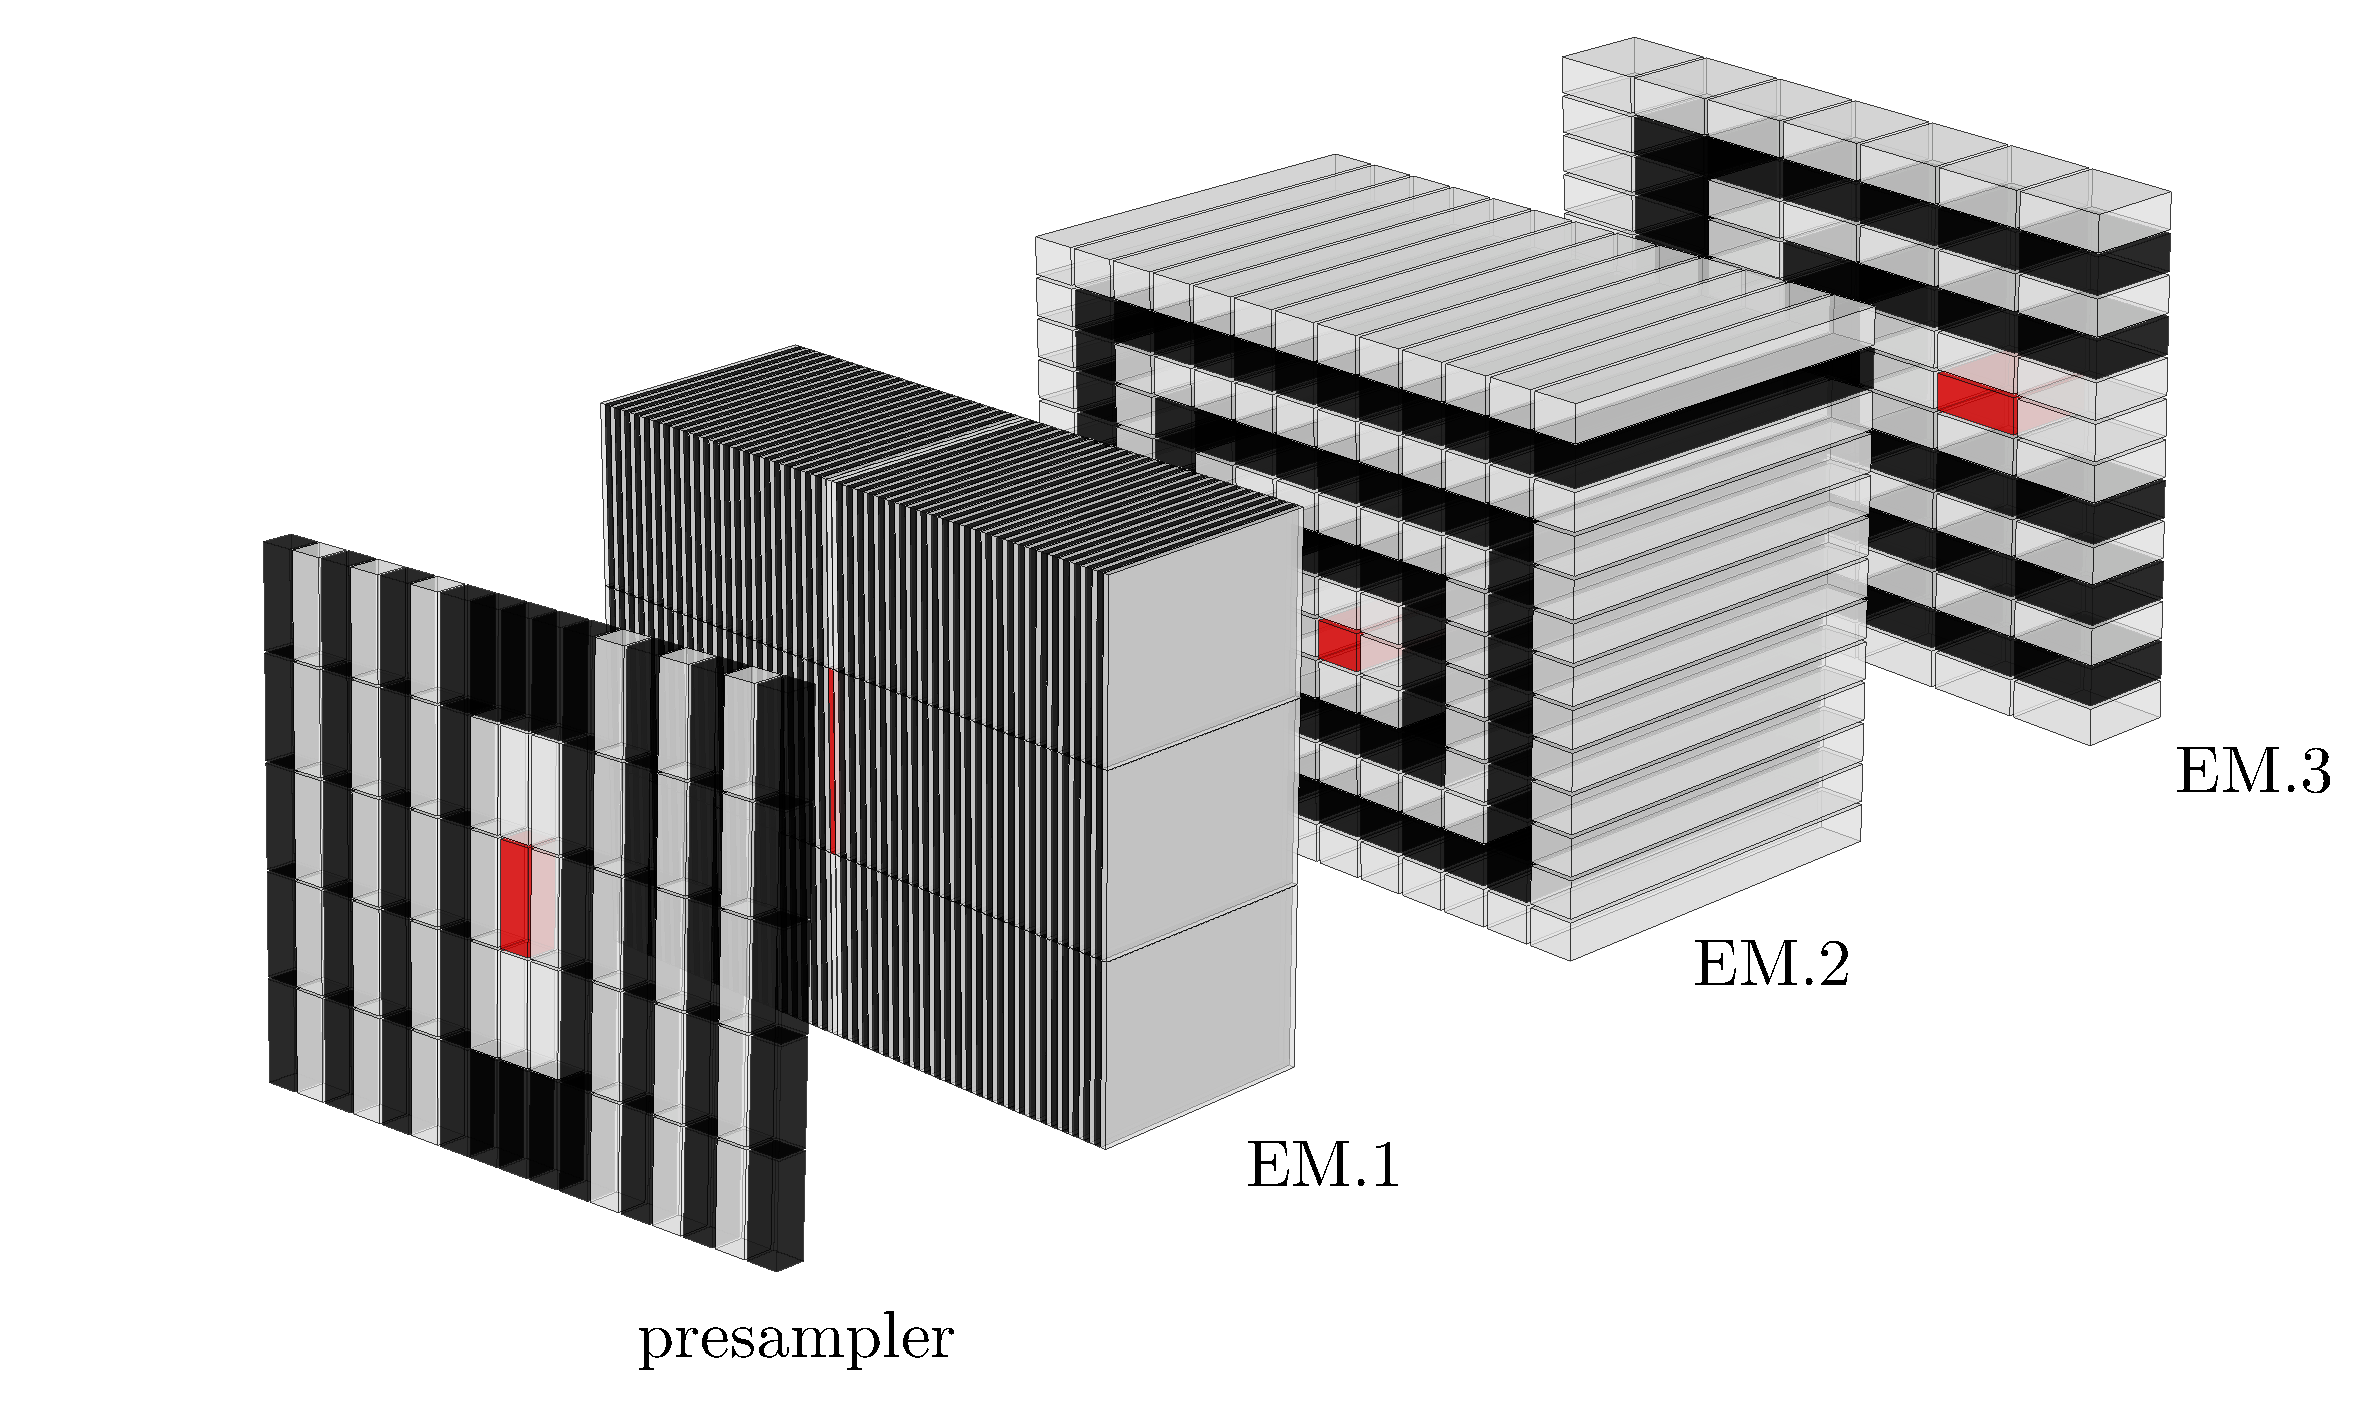
\includegraphics[width=\textwidth]{sections/02_context/figures/ATLAS_EM_Layers_v5.pdf}
			\caption{Eletromagnetic calorimeter cells within the ringer reconstruction window.}
		\end{subfigure} \\
		\begin{subfigure}[c]{0.8\textwidth}
			\centering
			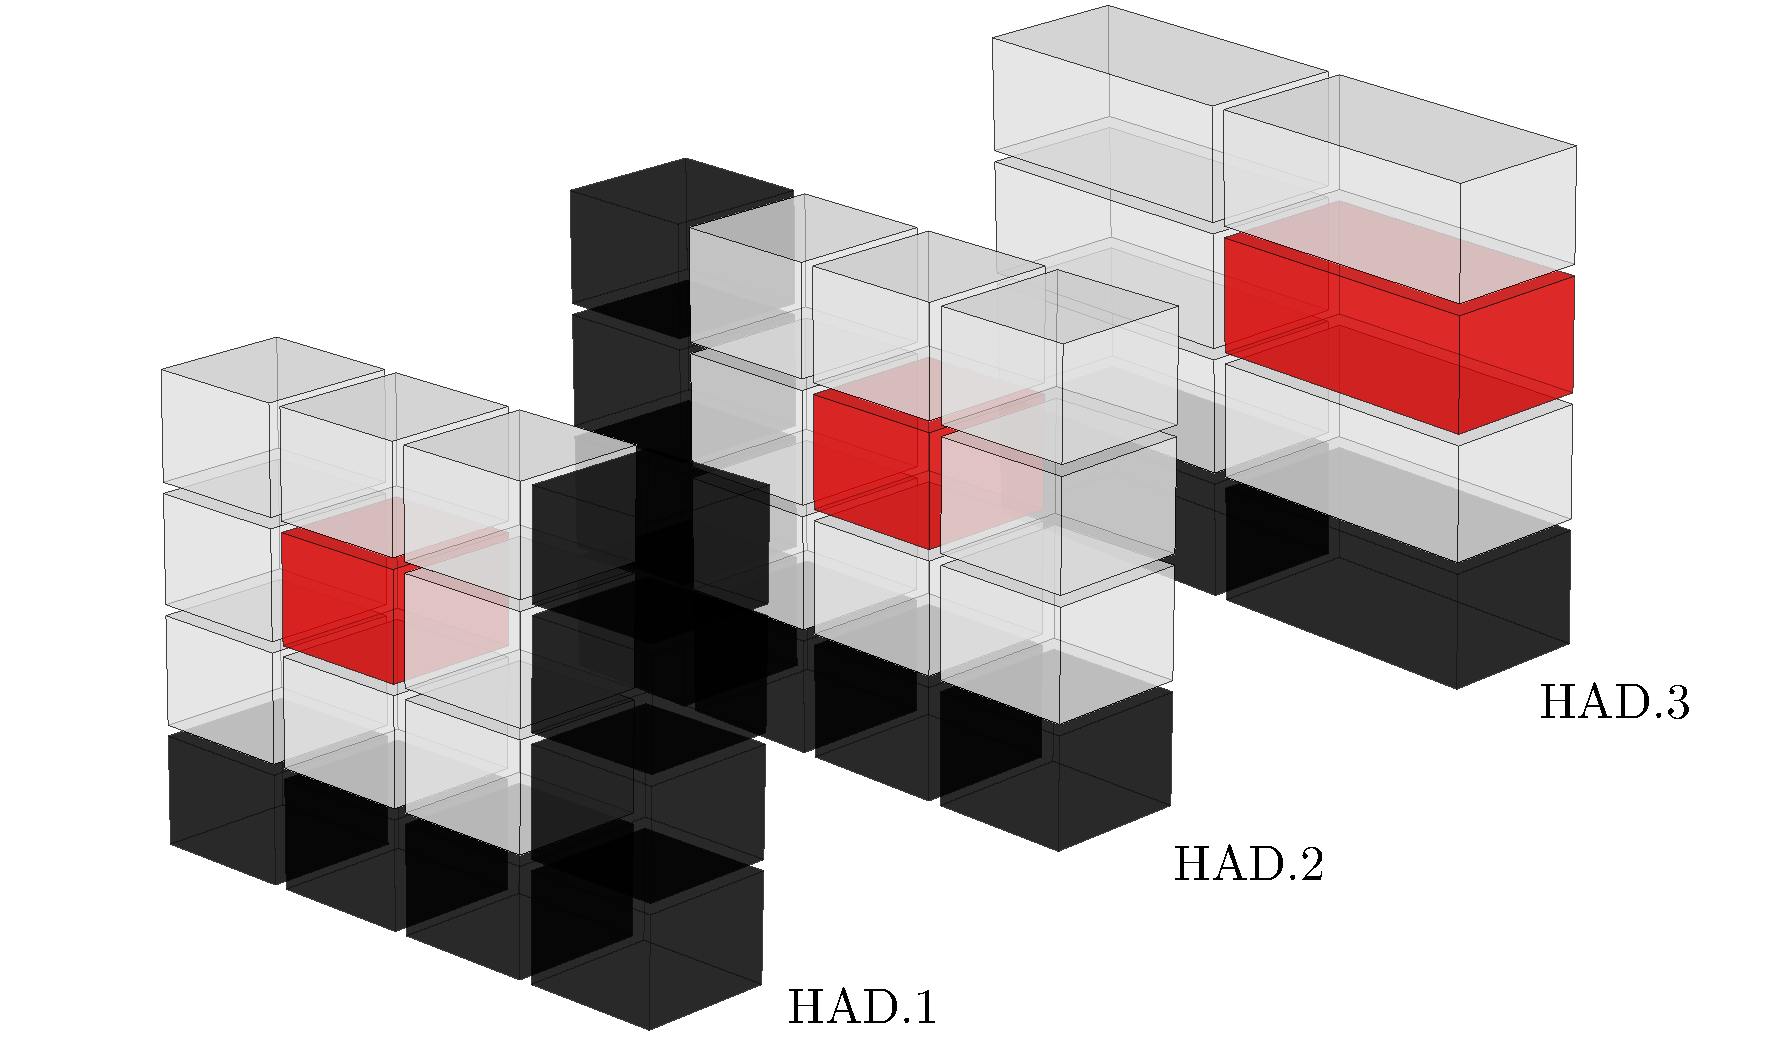
\includegraphics[width=\textwidth]{sections/02_context/figures/ATLAS_HAD_Layers_v5.pdf}
			\caption{Hadronic calorimeter cells within the ringer reconstruction window.}
		\end{subfigure}
	\end{center}
	\caption{\label{fig:calo_rings}
		Sketch to illustrate the ring-shaped energy description. See
		Section~\ref{top:algorithm} for more details. 
		The most energetic cell is in red, while the consecutive neighbouring rings are represented by alternating gray and black cells.
	}
\end{figure}


The ring building process covers the whole $0.4\times0.4$ (\etaphi axis) RoI
seeded by \licalo, resulting in 100 rings in total across all calorimeter layers.
Thereby, a dimensionality reduction is provided by compacting
typical input space dimensionality of approximately 1000--1200 cells per ROI into
the above-mentioned 100 rings through the usage of EM shower physics knowledge: the rings can keep a complete description of the symmetric lateral and
longitudinal information. However, the algorithm only approximates this concept
in order to meet the online operation requirements and avoid further
manipulation of the instrumented information. The full description and
discussion on the current algorithm are addressed in
Section~\ref{top:algorithm}.



Conceptually, the ring structure aims at exploiting the concentric nature of energy depositions in the calorimeter and the corresponding symmetry in the development of the shower.  Adding the calorimeter cells belonging to a given ring and, thus producing the ring sums, makes it possible to improve the signal-to-noise ratio from individual cells, especially in the tail of the energy distributions along the calorimeter layers.  Moreover, a nonlinear discriminant may profit from the statistical fluctuations in shower development, which are captured by means of the rings' profile, and provide efficient electron selection even in high pileup conditions.

Nonetheless, some observations concerning the description of a shower through rings are worth making. First, the standard shower shape variables, or simply shower shapes, cannot be obtained through operations starting from the rings.  Thus, the rings represent an alternative for shower development description and not a possible replacement for the shower shapes.  Therefore, a strategy considering both rings and shower shapes might explore a complementary discriminating information in the future.



Second, one should also notice
that the rings do not use the same sensors more than once for each variable.
This is not strictly true for the shower shapes, although it is fairly unusual.
In contrast, pattern recognition through modern machine learning
algorithms~\cite{Engelbrecht2007,Goodfellow2016}, as convolution
neural-networks~\cite{Gu2018}, build variables processing several times
the same sensors. Additionally, as providing dimension reduction and keeping the physics interpretation of the shower development, the shower shapes are also suited to bringing insights through uni-variate analysis carried out on each
single dimension composing the input space.
Thus, an alternative ring-based trigger strategy was developed and the shower shapes were used to evaluate how the physics properties of the showers were captured by the neural networks trained on calorimeter information formatted into ring sums. 









\section{Electron Triggers}\label{ssec:egamma_trigger}


Electron triggers~\cite{aad2020performance} begin with
the search for an EM energy deposit in the calorimeter with a \licalo{} sliding
window algorithm ~\cite{Franchino:2730851} using coarse granularity calorimeter information, in order to
fulfill the targeted latency requirements in $2.5\mu s$. This selects a RoI of $0.4\times 0.4$
in the $\eta\times\phi$ plane and applies a minimal transverse energy and object
multiplicity requirements, which depend on the trigger
specifications~\cite{TRIG-2016-01}.
 
The \hlt{} selection starts with the fast calorimeter reconstruction
step (\fastcalo), which has two implementations
(Figure~\ref{fig:ringer_chains}): the original cut-based algorithm; and one based on the Ringer algorithm. 
This processing step is followed by the fast track reconstruction
(\fastelectron), which applies restrictions on variables that indicate the quality of proximity matching between the electron candidate positions reconstructed from the track and the calorimeter. Due to its high-demanding computational algorithms, early removal of fake candidates can be used to reduce the relatively high CPU resources needed for this selection stage.


\begin{figure}[h!tb]
  \begin{center}
  %\hspace{0.01\textwidth}
  \begin{subfigure}[c]{.48\textwidth}
  \centering
  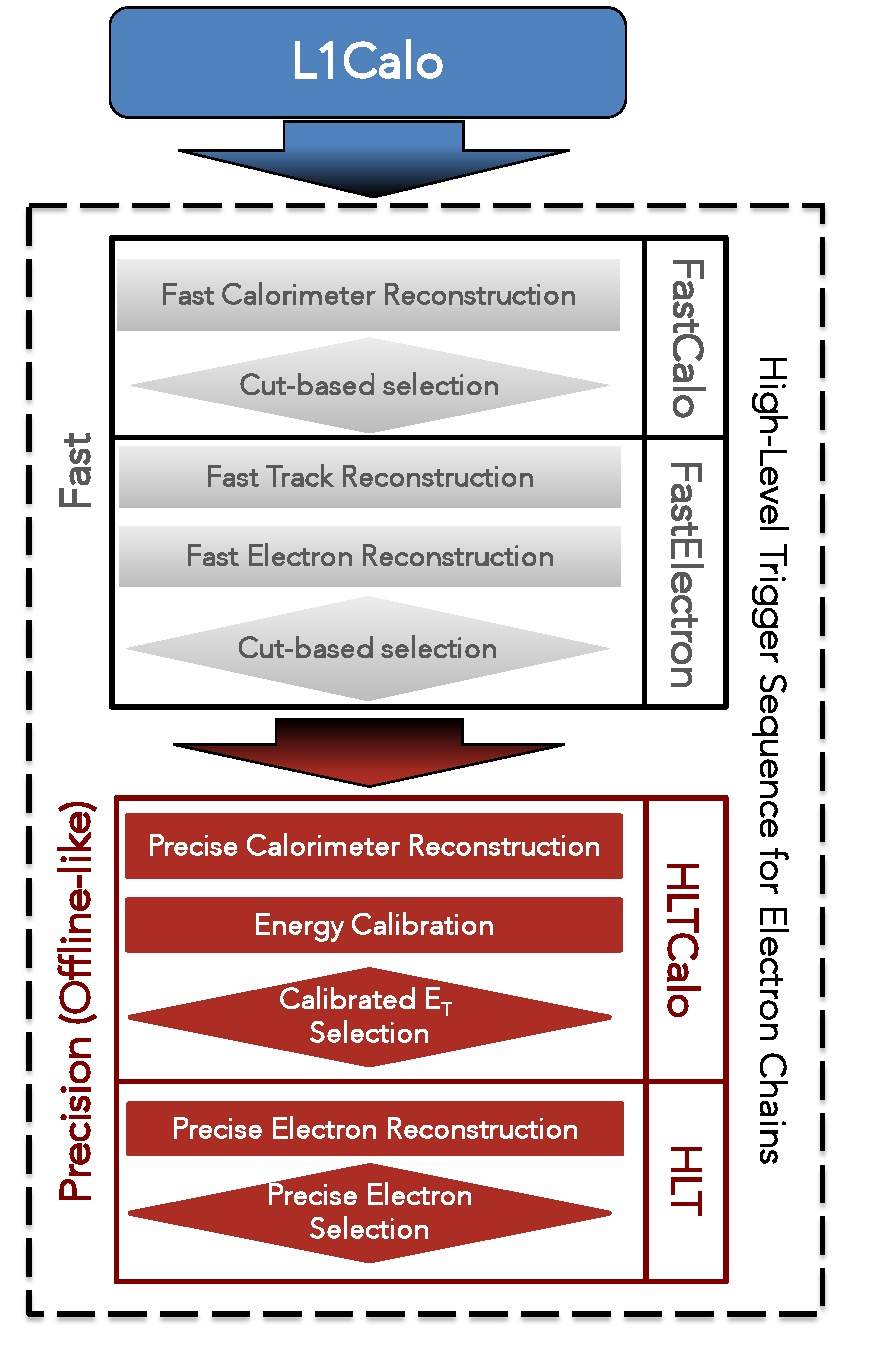
\includegraphics[width=\textwidth]{sections/02_context/figures/ElectronChain_Run2_cutbased.pdf}
  \caption{noringer chain (2017).}
  %\label{fig:cutbased_chain}
  \end{subfigure}
  \hfill
  \begin{subfigure}[c]{.48\textwidth}
  \centering
  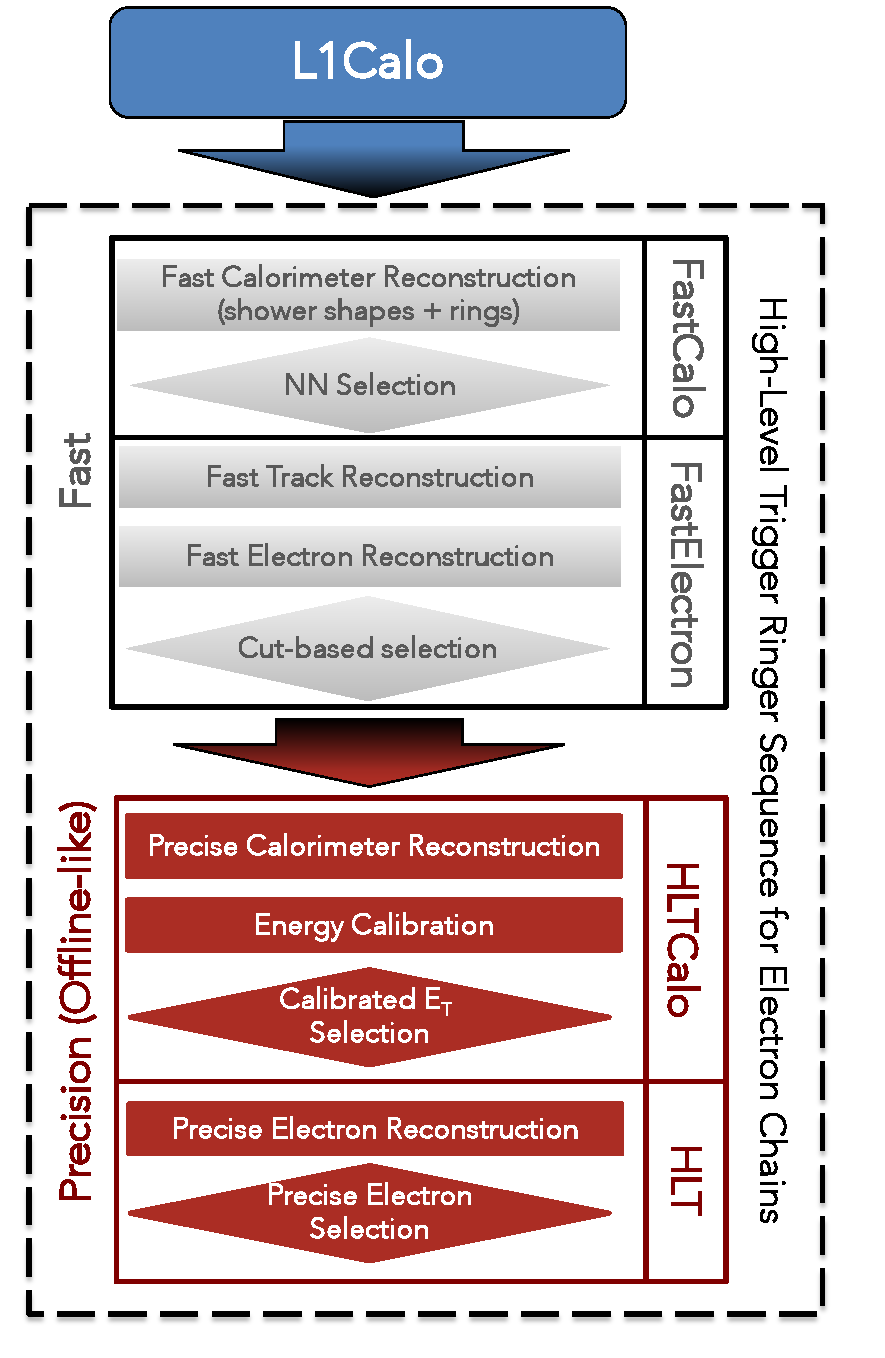
\includegraphics[width=\textwidth]{sections/02_context/figures/ElectronChain_Run2_ringer.pdf}
  \caption{ringer chain (2017).}
  %\label{fig:ringer_chain}
  \end{subfigure}
  %\hfill
  \caption{Comparison of the processing flow diagrams for the electron triggers. (a)
  contains the logic employed in the triggers based on the cut-based strategy
  (noringer) in the \fastcalo step. (b) contains the primary electron
  chains (ringer chains) since 2017, with the \rnn{} algorithm.}%
  \label{fig:ringer_chains}
  \end{center}
\end{figure}

% TODO Remove column (c) or use the note table
  
  

% http://acode-browser1.usatlas.bnl.gov/lxr/source/aa/Trigger/TrigHypothesis/TrigEgammaHypo/python/TrigL2CaloHypoCutDefs.py

A precise electron candidate energy is later computed (\hltcalo). Final HLT selection makes use of a likelihood
approach~\cite{ATL-COM-PHYS-2017-1012,ATLAS-PERF-2017-01-002}, based on the estimation of marginal probability density function (pdf) for the discriminating variables ($\vec{x}$) given in Table~\ref{tab:IDcuts}. The discriminant value is computed by:


%, which is built using adaptive Gaussian Kernel Density Estimation (KDE)~\cite{Silverman2018,TMVA}. The
%resulting kernels, obtained (since 2017) from runs of the previous year, and
%earlier from simulation data, are approximated by histograms with thin
%granularity (generally employing 500 bins) and then interpolated to give the
%signal and background probability values computed for the $i$th variable ($P_{s(b),i}(x_i)$). 


\begin{equation}
  d_{\mathcal{L}} = \frac{\mathcal{L}_{s}}{\mathcal{L}_{s} + \mathcal{L}_{b}},
\end{equation}
  
\noindent where
  
\begin{equation}
\mathcal{L}_{s(b)}(\vec{x}) = \prod_{i=1}^{n} P_{s(b),i}(x_i).
\label{eq:likelihoods}
\end{equation}



\noindent and $P_{s(b),i}(x_i)$ is the signal (or background) probability values computed for the $i$th variable. Roughly\footnote{A transformation is employed to allow
easier computation of the proper threshold~\cite{aaboud2019electron}.},
the decision is made by comparing $d_{\mathcal{L}}$ with a
threshold linearly corrected for \avgmu{}, in order to mitigate electron trigger
efficiency loss due to pile-up the effect caused by proton-proton collisions in the same or surrounding bunch crossings. The mean number of interactions per crossing (\avgmu{}) corresponds to the
mean of the Poisson distribution of the number of interactions per crossing calculated for each colliding bunch pair. In addition, some other requirements are
applied on specific variables (e.g., number of hits at Pixel detector, $\Delta\eta$, $\trackdO$, $\deltapoverp$) to improve the final decision~\cite{aaboud2019electron}

To account for detector response evolution with
respect to \Et\footnote{Projection of the energy ($E$) in the transverse plane,
computed by $E\cdot\sin(\theta)$ or $E\cdot\cosh(\eta)$.} and
$\eta$, both the Kernel Density Estimation (KDE) and discriminant requirements are computed in delimited ($\eta\times E_{T})$
regions in this plane (boundaries defined in the Section~\ref{top:nn_ensemble}).
A finer-grained grid in \Et is employed for the derivation of the discriminant
requirements to obtain a relatively smooth efficiency transition. Additionally,
both pdf values and discriminant requirements near the boundaries are determined
using a linear interpolation of the neighbouring bins to avoid large
discontinuities in signal efficiency~\cite{aaboud2019electron}.

Finally, the discriminant requirements are optimized for four working points
which can be used to define triggers targeting different combinations of the desired output rate
and required efficiency. The \tight{} operating point prioritizes the purity of
collected electron candidates and demands lower output rate.
The \loose{} and the \vloose{} operating point emphasize potential electron observations, resulting in higher output rate with substantial lower purity. 
On the other hand, the \medium{} working point allows an intermediate
operation between both strategies. Each operating point also leads to
variation in the physics composition (e.g., light- and heavy-flavour, photon
conversions) of background triggered samples. 








 % need to fix tables and alg
\chapter{The \rnn{} Algorithm}%
\label{sec:neuralringer}

This section describes the \rnn{} concepts and the resulting algorithm used for Run~2
operation. Considerations about data sets (Section~\ref{ssec:dataset}) and the \TnP method
(Section~\ref{ssec:tnp}) employed to extract signal and background samples
from real ATLAS data start this section. Section~\ref{ssec:rnn_for_online_and_eletrons} refers to the
decisions made for the \rnn{} development in order to optimize its contributions in saving processing resources. Aiming at better exploring the discriminative
power of ring sums for electron triggers (Section~\ref{ssec:ringer_id}),
an ensemble of neural-networks is employed. Its training procedure and how trigger decisions are made are covered in Section~\ref{sec:tuning}.




\section{Data sets and Event Selection}%
\label{ssec:dataset}

The training procedure for 2017 operation was built with samples of 2015 simulated $Z\rightarrow ee$ decay selected by the $Z\rightarrow ee$ \TnP method (see Section~\ref{ssec:tnp}). Background samples for electron processes were simulated. A filter was applied to enrich the sample in electron backgrounds selecting events which have particles produced in the hard scatter with a summed transverse energy exceeding 17 GeV in a region of $\Delta\eta\times\Delta\phi=0.1\times0.1$. During 2016 data taking, the pile-up peak reached was 40 interactions per bunch crossing.
Here, both simulated data include a pile-up of 60 interactions in average, per bunch crossing which has never been seen before in collision data.

After the training stage, the decision is taken by applying a threshold. To set the correct value without causing any inefficiency in the end of the HLT in data, the full \textit{pp} collision data set recorded by ATLAS in 2016 with LHC operating at a centre-of-mass energy of $\sqrt{s}=13 \text{TeV}$ during of Run 2 was used. The electrons where selected by $Z\rightarrow ee$ \TnP method and the offline tight criteria. For background, objects rejected by the $Z\rightarrow ee$ \TnP method, that does not belong to any tag-probe electron pair, and reproved by the loosest offline available criteria were used. For the 2018 operation, the purely data-driven strategy was used, selecting events from the 2017 recorded data to train the models and adjust all thresholds.

The tuning and analysis performed on data recorded have their quality ensured by the data quality procedure. To facilitate the large data manipulation, events of potential interest are derived using specific requirements providing potential \Zee{} \tnp{} candidates and background electrons. 

%
\begin{table}[ht!]%\footnotesize
\centering
\caption{Event selection for tuning the models and defining the discriminant
requirements of the \rnn operating in the Run 2. Symbol ``\veto'' is used to
indicate that the physics object is considered when it is rejected by the
criterion. The label `mc15' corresponds to simulated data based on Monte Carlo
algorithms and `Tier0' correspond to ATLAS experimental
data \cite{aad2020performance}.}\label{tab:event_selection}
% TODO Explain why not loose and not Zee
\resizebox{\textwidth}{!}{%
\begin{tabular}{lp{6.8cm}cc}
\hline \hline
Type & Dataset & \TnP & Offline Selection \\
\hline \hline
\multicolumn{4}{c}{2017 Models} \\
\hline
signal &
mc15\_13TeV.361106.PowhegPythia8EvtGen\allowbreak{}\_AZNLOCTEQ6L1\_Zee.merge.AOD.\allowbreak{}e3601\_s2876\_r7917\_r7676
& \Zee & None \\
background &
mc15\_13TeV.423300.Pythia8EvtGen\allowbreak{}\_A14NNPDF23LO\_perf\_JF17.merge.AOD.\allowbreak{}e3848\_s2876\_r7917\_r7676
& None & None \\
\hline
\multicolumn{4}{c}{2017 Discriminant Requirements} \\
\hline
signal & 2016 Tier0 + EGAM1 (p3013) + GRL v88 & \Zee & \tight \\
background & 2016 Tier0 + EGAM7 (p3013) + GRL v88 & \veto\Zee & \veto\loose \\
\hline
\multicolumn{4}{c}{2018 Models and Discriminant Requirements} \\
\hline
signal & 2017 Tier0 + EGAM1 (p3336) + GRL v97 & \Zee & \tight \\
background & 2017 Tier0 + EGAM7 (p3336) + GRL v97 & \veto\Zee & \veto\vloose \\
\hline \hline
\end{tabular}
}
\end{table}




\subsection{\TnP Method}\label{ssec:tnp}

The \tnp{} method~\cite{PERF-2016-01} selects, from a known resonances such as \Zee{}, an unbiased sample of `probe' electrons by using strict selection requirements on the second `tag' object. For electrons coming from $Z$ boson decay, the selection of two EM objects with an invariant mass around the $Z$ mass with opposite charge is enough to get a pure sample of electrons as soon as one of those objects is tagged as a well-identified electron. The remaining object can them be assumed to be an electron with a very high underlying purity. This object can them be used as a probe to test the electron trigger efficiency. The selection of the tag particle is done according to offline analysis criteria to make sure that the trigger selection introduces a minimal loss of those events at the final physics analysis level~\cite{aaboud2019electron}. A single electron is used as a tag to select the event at the trigger level, allowing the second electron to be used as a probe to measure trigger algorithm performance~\cite{aad2020performance}.


\section{Algorithm Development}\label{ssec:rnn_for_online_and_eletrons}

The \rnn{} algorithm was initially proposed for electron-jet discrimination. 
During Run 2, both online and offline versions
were considered for  development, but the scarcity of available human resources restricted the scope of developments, which focused on reducing CPU demands of the online electron triggers. Within the electron triggers, \hlt{} selection is
specially relevant to single object triggers, which, in turn, use the most of the trigger bandwidth~\cite{aad2020performance}. Particularly, the primary single electron triggers
are currently evaluated and developed using \Zee{} \tnp{} samples 
(Section~\ref{ssec:tnp}), in which most electrons have $\et>\SI{15}{\GeV}$, which is the region of interest in physics studies and on which the \rnn{} developments focus. The result of this effort
follows.


\subsection{Building the Rings}\label{top:algorithm}

The ATLAS calorimeters comprise rectangular cells in the
\etaphi plane for different layers in depth\footnote{Except for the forward calorimeters.}. Thus, an actual circular structure cannot be defined
without intensive processing of the cell energy information. As the algorithm was
considered to operate online, approximations were made. Especially, the rectangular structure of
the rings follows the instrumentation and the ring coverage is bounded to the RoI area. In addition, granularity changes from the cell sizes from different regions of the detector are neglected in order to employ a grid-like algorithm.


Here, the algorithm RoI covers a
region of the calorimeter, centered in the L1 provided RoI, of
$0.4\times0.4$ in the $\eta\times\phi$ plane. The algorithm
starts on the second EM sampling layer (EM2)\footnote{This convention is used for all sampling layers, thus HAD1 stands for the first hadronic layer, HAD2 the second hadronic layer etc.}, where position given in $\eta\times\phi$ plane of the cell with
highest $E_T$ on the algorithm RoI is taken as the center of the cascade
interaction in the calorimeter. The initial seed cell position is propagated to other calorimeter layers in order to define the axis of the rings in that layer. Then, for each layer, the algorithm refine the seed position searching for most energetic cell inside of the window centered by the EM2 initial seed. The refined seed ($c_{hot,l}$) will be used as starting point to build the rings. A ring $R_{n,l}$ contains all cells in calorimeter layer $l$ which are $n$ cells from the refined seed (See Figure~\ref{fig:building_rings_a} for an illustration of the parameters). Formally,


\begin{equation}
%\label{eq:ring_idx}
R_{n,l} = \left\{c_{n,l} \mid n = \left\lfloor \max{\left( 
\frac{| \eta_{i,l} - \eta_{hot,l} |}{h_{\eta,l}}, 
\frac{| \phi_{i,l} - \phi_{hot,l} |}{h_{\phi,l}} 
\right)} \right\rceil, 
\forall c_{i,l} \in
\Theta_{RoI,l}
\right\},
\end{equation}



\noindent where (analogous to $\phi$ when suitable): $\eta_{i,l}$
and $\eta_{hot,l}$ are respectively the $c_{i,l}$ and $c_{hot,l}$
cells position in $\eta$; $h_{\eta,l}$ is the $l^{th}$ layer cell size in $\eta$; $\Theta_{RoI,l}$ is the set of cells
in the $l^{th}$ layer which are within the Ringer RoI.
\tablename~\ref{tab:ring_alg_parameters} shows the number rings computed at each layer and the respective granularity.


\begin{table}[ht!]
\centering
\caption{Nomenclature defining the \rnn{} algorithm layers and sections, as well
  as the respective parameters employed and calorimeter sampling
  layers from which the cells are extracted. The \rnn{} algorithm
  parameters are dependent on the ringer layer $l$ and independent on \eta{} and
  \et{} during Run~2. The parameters are the ring size in \eta{}
  ($h_{\eta,l}$), $\phi$ ($h_{\phi,l}$) and the number of rings to be computed
  in each layer ($\text{N}_l$). 
  %The values for $h_{\etaa,l}$ and $h_{\phii,l}$
  %are approximated, the exact ones can be obtained for $\eta=0$ in
  %Table.
%To refer to a ring, it will be used notation XYYY, where X is the ring index in
%the YYY layer.
}%
\label{tab:ring_alg_parameters}
\resizebox{.8\textwidth}{!}{%
\begin{tabular}{lc|ccc|ccc}
\hline
\hline
\multicolumn{2}{c|}{Ringer} & \multicolumn{3}{c|}{Calorimeter Sampling} & 
\multicolumn{3}{c}{Parameters} \\
\hline
Section & Layer ($l$) & Barrel & \itc & End-cap & $h_{\etaa,l}$ & $h_{\phii,l}$ & $N_l$ \\
\hline
\hline
\multirow{4}*{EM} & \ps &  \presamplerb & & \presamplere & 0.025 & 0.1 & 8 \\
\cline{2-5}
& \emi & \emb{1} &  & \emec{1} & 0.003 & 0.1 & 64  \\
\cline{3-5}
& \emii & \emb{2} &  & \emec{2} & 0.025 & 0.025 & 8 \\
\cline{3-5}
& \emiii & \emb{3} &  & \emec{3} & 0.050 & 0.025 & 8 \\
\cline{1-5}
\multirow{6}*{HAD} & \multirow{2}*{\hadi} & \tilebar{0} &
\multirow{2}*{\tilegap{3}} & \multirow{2}*{\hec{0}} & \multirow{2}*{0.1} & \multirow{2}*{0.1} & \multirow{2}*{4} \\
&                     & \tileext{0} &                               &                           \\
\cline{3-5}
& \multirow{2}*{\hadii} & \tilebar{1} & \multirow{2}*{\tilegap{1}} & \hec{1}       & \multirow{2}*{0.1} & \multirow{2}*{0.1} & \multirow{2}*{4} \\
&                   & \tileext{1} &              & \hec{2}  \\
\cline{3-5}
& \multirow{2}*{\hadiii} & \tilebar{2} & \multirow{2}*{\tilegap{2}} & \multirow{2}*{\hec{3}} & \multirow{2}*{0.2} & \multirow{2}*{0.1} & \multirow{2}*{4} \\
&                     & \tileext{2} &                &             \\
\hline
\hline
\end{tabular}
}
\end{table}






If no cell is available for a given ring, the correspondent ring
quantity is set to 0.
The sum of the transverse energies of cells $c_{n,l}$ in the ring $R_{n,l}$ form a vector of discriminating quantities. 
They are ordered outwards and from the
innermost layer of the calorimeter and provided the ring-shaped information 
of the RoI. Figure~\ref{fig:building_rings_b} shows the ring-shaped mean profile differences between electrons and jet particles. The implementation of this algorithm is simple and the actual code
was optimized to be fast (see Section~\ref{top:fastcalo_cpu}). 









%%%% Coloring the comment as blue
\newcommand\mycommfont[1]{\footnotesize\ttfamily\textcolor{blue}{#1}}
\SetCommentSty{mycommfont}
\SetKwInput{KwInput}{Input}                % Set the Input
\SetKwInput{KwOutput}{Output}              % set the Output



\begin{algorithm}[H]

    %\DontPrintSemicolon
  
    \KwInput{$\Theta_{RoI,l}$, $\eta_{cluster}$, $\phi_{cluster}$, $h_{\eta,l}$, $h_{\phi,l}$, $N_{l}$}
    \KwOutput{r}

    r $\leftarrow$ initialize with zeros the ring vector with size $N_{l}$
 
    \tcc{Energy, $\eta$ and $\phi$ from the hottest cell.}
    $E_{hot,l}$, $\eta_{hot,l}$, $\phi_{hot,l}$ = 0

    \tcc{Refine the hottest cell position around the cluster center position.}
    \For{$C_{i,l}$ $\leftarrow$ $\Theta_{RoI,l}$}
    {
        $E_{i,l}$ $\leftarrow$ energy from $C_{i,l}$

        $\eta_{i,l}$ $\leftarrow$ central position in $\eta$ from $C_{i,l}$
        
        $\phi_{i,l}$ $\leftarrow$ central position in $\phi$ from $C_{i,l}$

        \tcc{Check if the current cell ($C_{i,l}$) is inside of a window with $0.4\times0.4$.}
        \If{ $(\eta_{cluster}-0.2)$ > $\eta_{i,l}$ e $\eta_{i,l}$ < $(\eta_{cluster}+0.2)$}
        {
            \If{ $(\phi_{cluster}-0.2)$ > $\phi_{i,l}$ e $\phi_{i,l}$ < $(\phi_{cluster}+0.2)$}
            {
                \If{$E_{i,l} > E_{hot,l}$}
                {
                    $E_{hot,l}$ $\leftarrow$ $E_{i,l}$

                    $\eta_{hot,l}$ $\leftarrow$ $\eta_{i,l}$
                    
                    $\phi_{hot,l}$ $\leftarrow$ $\phi_{i,l}$
                }
            }
        }
    }


    \tcc{Fill the energy of each ring using the hottest cell position as the center.}
    \For{$C_{i,l}$ $\leftarrow$ $\Theta_{RoI,l}$}
    {

        $\eta_{i,l}$ $\leftarrow$ central position in $\eta$ from $C_{i,l}$
        
        $\phi_{i,l}$ $\leftarrow$ central position in $\phi$ from $C_{i,l}$

        $\delta_{\eta}$ = $(\eta_{i,l}-\eta_{hot,l})/h_{\eta,l}$

        $\delta_{\phi}$ = $(\phi_{i,l}-\phi_{hot,l})/h_{\phi,l}$

        $n = round(max(\delta_{\eta}$, $\delta_{\phi}))$
                
        \If{n $\leq$ $N_{l}-1$}
        {
            $E_{i,l} \, \leftarrow$ energy from $C_{i,l}$

            $r[n] += E_{i,l}$

        }  
    }
    
    \tcc{Calculate the transverse energy for each ring given $\eta_{hot,l}$}
    \For{ i = 0; i < $N_{l}$; i++}
    {
        $r[i] = \frac{r[i]}{\cosh(|\eta_{hot,l}|)}$
    }

  \Return{r}


\caption{Rings build algorithm.}
%\label{alg:ringer_alg}
\end{algorithm}




\begin{figure}[!ht]
  \begin{center}
  \begin{subfigure}[c]{.48\textwidth}
  \centering
  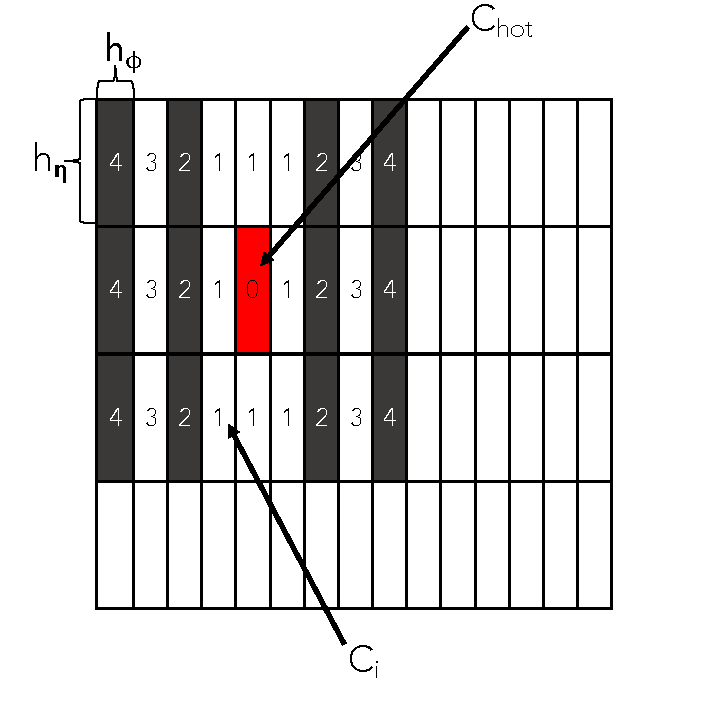
\includegraphics[width=\textwidth]{sections/03_ringer/figures/reco_steps/ring_em1_mask.pdf}
  \caption{}
  \label{fig:building_rings_a}
  \end{subfigure}\\
  \centering
  
  \begin{subfigure}[c]{.7\textwidth}
  \centering
  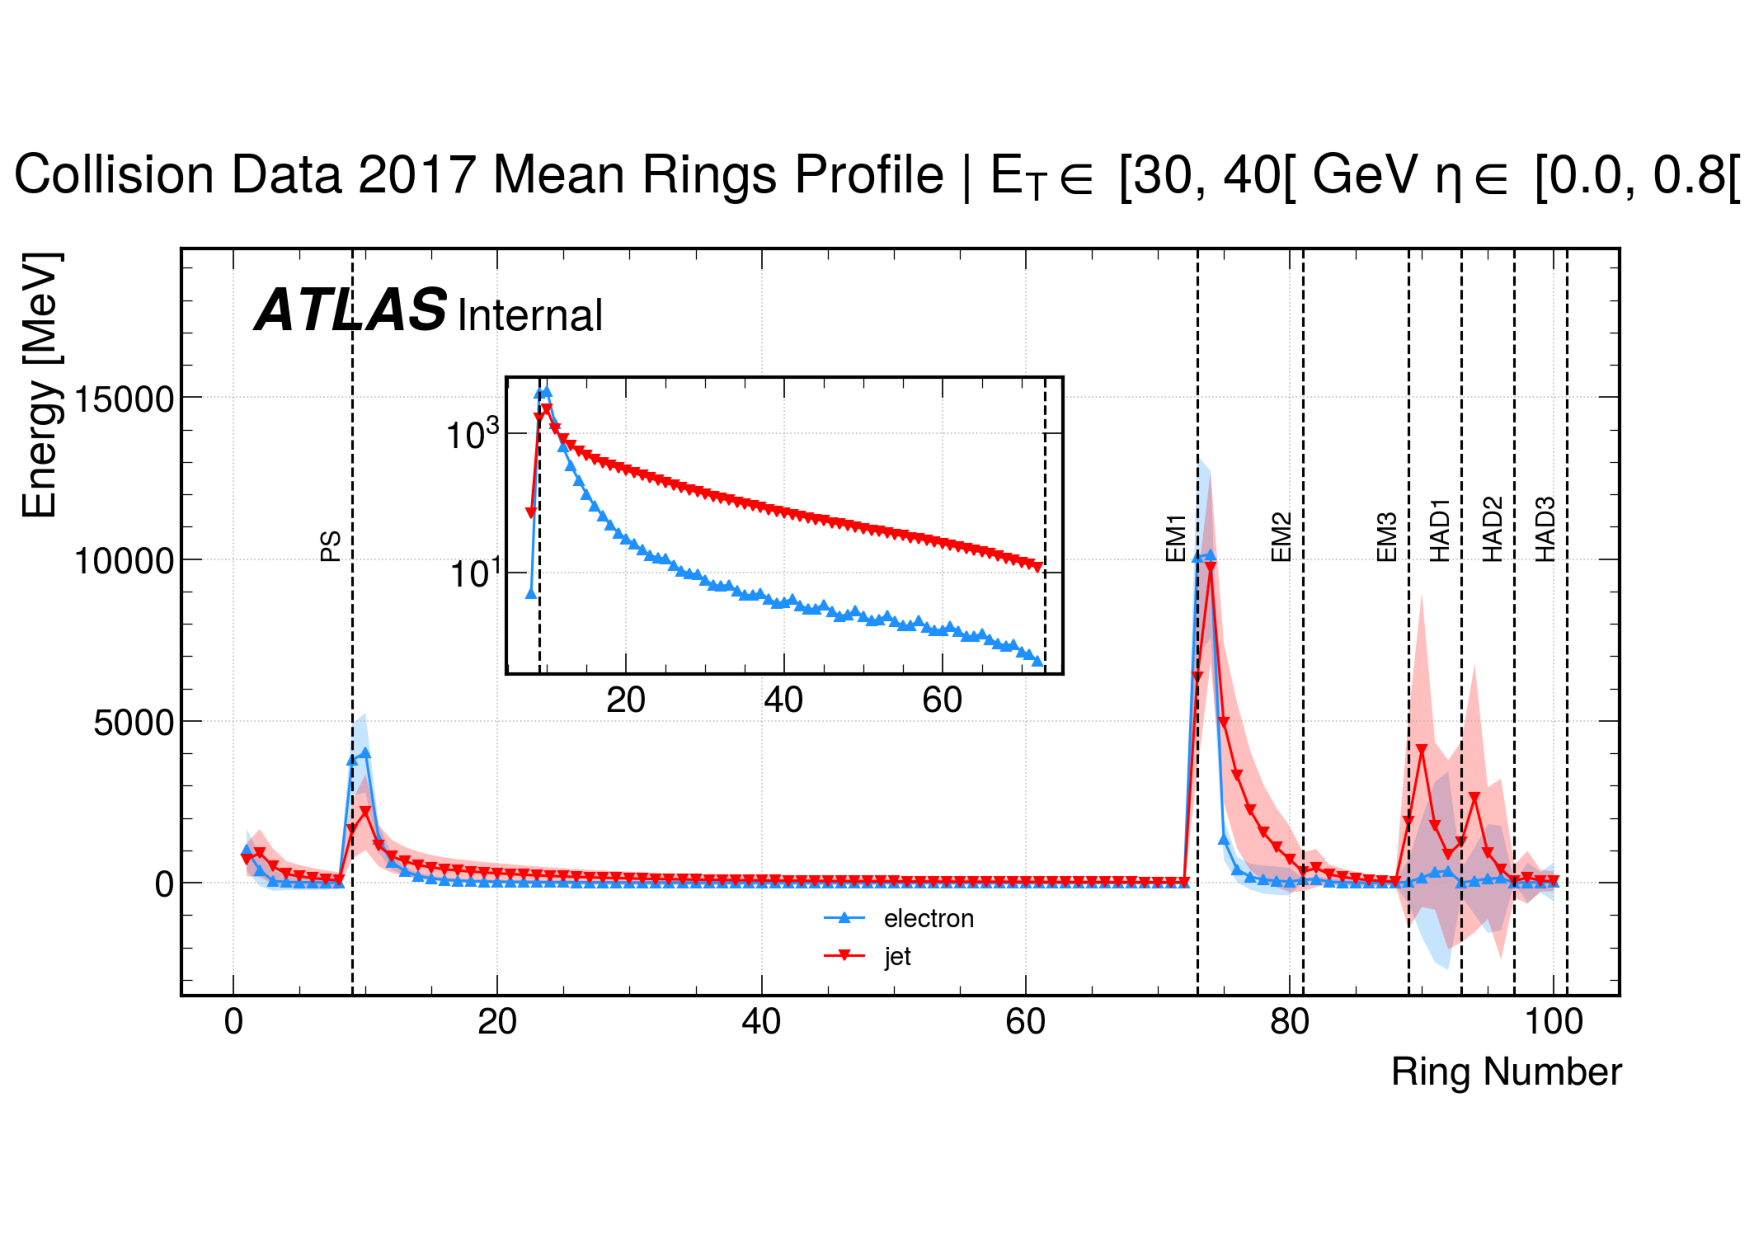
\includegraphics[width=1.1\textwidth]{sections/03_ringer/figures/reco_steps/data17_zee_mean_rings_profiles_et2_eta0.pdf}
  \caption{}
  \label{fig:building_rings_b}
  \end{subfigure}
  \caption{
  Top: illustration of the \fastcalo algorithm for building ring sums in the EM1, sketching of the computation of $n$ for the first four rings in a hypothetical layer.
  	Bottom: average rings profile from collision data at $30 \leq E_T < 40$ GeV and $0.0 \leq \eta < 0.8$ for each layer of the calorimeter. The embedded profile shows the EM1 layer rings in a logarithmic scale. Here, it is possible to observe that most part of the energy for the electrons is absorbed by the eletromagnetic layers. For the jets, the opposite is observed and most part of the energy is absorved by the hadronic layers.}
  \end{center}
\end{figure}





\section{Ring Sums as Discriminant Variables}\label{ssec:ringer_id}

% TODO Add references of sucesfull aplications of NNs in other fields.

%The ring sums compose a space with distinct nature with respect to the standard
%shower shape variables, where the first contains higher redundancy between its
%variables. Although the use of univariate cuts or a likelihood model could be
%considered, they have limitations to explore concisely the statistical
%dependency.
To deal with the high redundancy between the ring variables, we benefit from machine learning processing to unveil the latent discriminating space, as in
the case of a Multi-layer Perceptron (MLP) neural-networks~\cite{haykin_2008},
employed for Run~2 operation. 
%MLPs require a normalization preprocessing step~\cite{haykin_2008} to adjust the input dynamic range to the neuron activation function employed (Section~\ref{top:pp}). 
An ensemble of MLPs was employed for operation by tuning and selecting
the models per regions of the \eteta space (Section~\ref{top:nn_ensemble}), whose
motivations are driven by physics, instrumentation and software 
engineering. The \rnn
%engineering. In the same way, \rnn 
decision making is also based on division of the phase space in regions, and the discriminant requirement is
computed as a linear function of \avgmu to pursue signal efficiency invariance
to pile-up contributions. 
The strategy to structure the MLPs,  and train the hyper-parameters of the ensemble and tune of discriminant requirements 
%The strategy, structure of the MLPs and hyper-parameters for training the ensemble and tuning of discriminant requirements 
are described in Section~\ref{sec:tuning}.

%\begin{figure}[h!t]
%\centering
%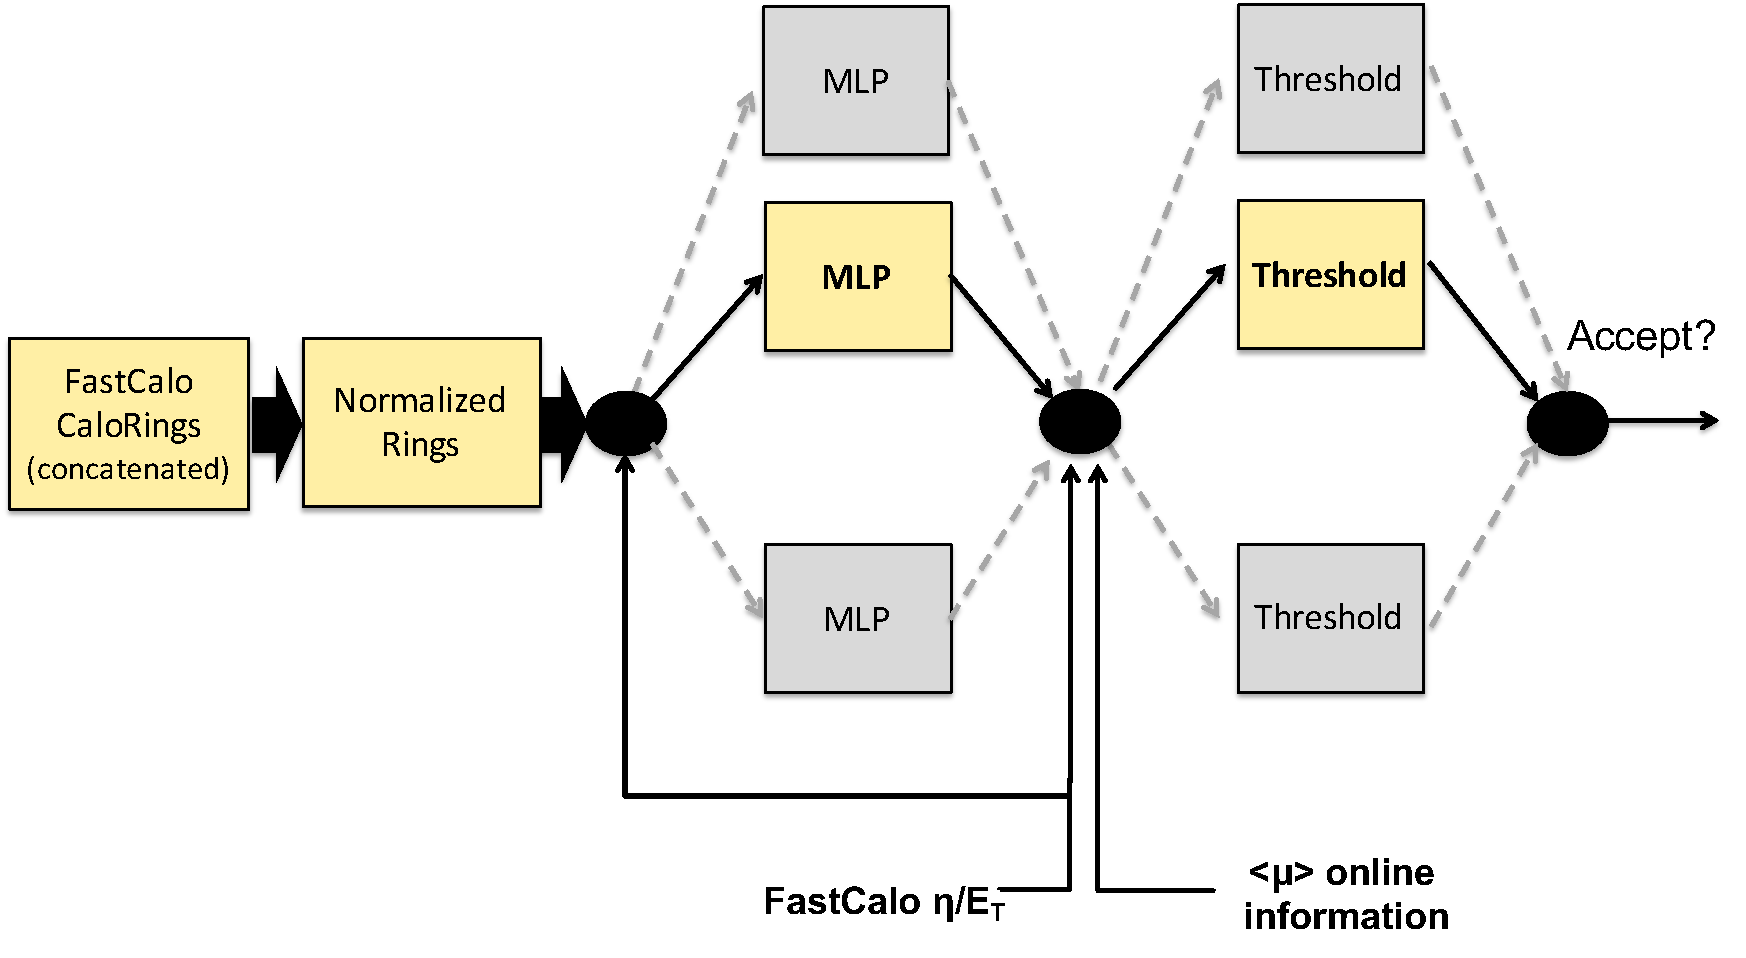
\includegraphics[width=0.9\textwidth]{sections/03_ringer/figures/Ensemble.pdf}
%\caption{\label{fig:ensemble}
%Processing flow diagram of the \rnn{} ensemble operation and decision making
%during Run~2.
%}
%\end{figure}

%
%%% Coloring the comment as blue
\newcommand\mycommfont[1]{\footnotesize\ttfamily\textcolor{blue}{#1}}
\SetCommentSty{mycommfont}
\SetKwInput{KwInput}{Input}                % Set the Input
\SetKwInput{KwOutput}{Output}              % set the Output



\begin{algorithm}[H]

    \DontPrintSemicolon
  
    \KwInput{Rings, $E_{T}$, $\eta$, \avgmu{}, models, thresholds}
    \KwOutput{Decision}

    Decision = False \tcc{Set the decision to false by default}
 
    \tcc{model is an object with attributes etmin, etmax, etamin, etamax and hold the neural network struture.}

    \For{model \leftarrow models}
    {
        % If et cluster is 
        \If{$E_{T}$ of the cluster is within the $E_{T}$ upper and lower bounds of the model}{
        {
            \If{$|\eta|$ of the cluster is within the $\eta$ upper and lower bounds of the model }
            {
                output $\leftarrow$ Propagate the normalized rings through the neural network and get the output}                
                \textbf{break}
            }

        }
    }
  

    \For{parameters \leftarrow thresholds}
    {
        \If{$E_{T}$ of the cluster is within the $E_{T}$ upper and lower bounds of the parameters }
        {
            \If{$|\eta|$ of the cluster is within the $\eta$ upper and lower bounds of the parameters}
            {
                \tcc{get the slope and offset parameters to apply the pileup corretion}
                \alpha $\leftarrow$ get slope from parameters

                \beta $\leftarrow$ get offset from parameters

                \tcc{check if output is higher than the threshold}
                \If {output > $\alpha\avgmu{}+\beta$}
                {
                    Decision = True \tcc{approve the event.}     
                }

                \textbf{break}
            }
        }
    }



\caption{Ringer ensemble algorithm}
\label{alg:ensemble}
\end{algorithm}


\subsection{Ring Sum Normalization}\label{top:pp}

The current strategy concatenates all rings in a single vector of 100
variables. An absolute normalization using the total RoI energy, as in
(\ref{eq:ring_norm}), is applied to normalize the variables. This procedure was
initially proposed and examined by~\cite{1995_seixas_ringer}, as a way of
preserving the shower energy profile in fractions of the total energy. The
absolute term is used to avoid reflecting the values along the axis due to
negative noise accumulation, a behavior which would impact the physics
representation of the normalized values and require a more complex decision
boundary:

\begin{equation}
  r^\prime_{k} = \frac{r_{k}}{| \sum\limits_{i=1}^{100} r_i
  |}, \;\;\;
    \forall \; k\in\{1,\dots,100\}.
\label{eq:ring_norm}
\end{equation}

A study on simulation data showed that this strategy had compatible
efficiency to other possible normalization schemes. It is specially valuable for its
simplicity as its making use of a non parametric approach, and for allowing easy interpretation of the shower profile. These reasons motivated its usage for Run 2.
%, however this strategy is subject to diminish signal contributions at stringent pile-up
%contamination, specially at low-energy operation due to lower signal-to-noise ratio.  
%Specifically, energy contributions from outer hadronic rings can
%dominate and deteriorate signal profile. We expect to review this strategy for
%Run~3, in particular when considering low-energy triggers ($<\SI{15}{\GeV}$).

\subsection{Motivation for an Ensemble of Neural Networks}\label{top:nn_ensemble}

The normalized concatenated ring vector feeds an ensemble of MLPs. A single
model is drawn from the ensemble for operation based on the nearest region on the \eteta space for which it was designed.
%In the following, we address the reasons for adopting such an ensemble.

In regards to calorimetry, the usage of an ensemble with specific models per
phase space region allows to mitigate fluctuations in the variable profiles
%(Figure~\ref{fig:ring_distortion}) 
due to the detector response and energy differences of the showers.
%response (Section~\ref{ssec:calo}). %and limitations of the online algorithm
%(Section~\ref{top:algorithm}) 
%in the observed signatures of the physics objects.
A large contribution comes from granularity changes, which are discrete
in the phase space. Other important factors 
influencing such profiles are the
amount of the material as a function of \abseta{} and the dependence of
underlying processes in the shower development with respect to the incoming
particle energy. Although these alterations are mostly continuous, it is also
possible to approach the problem using space discretization.

%Regions overlapping two distinct granularity are not handled by
%this approach. Other sources, as
%the variation in the shower profile due to the energy and amount of material
%(see Figures~\ref{fig:cal_em_x0} and~\ref{fig:cal_had_lambda}), contribute with
%modifications in the variable profiles that may not be completely mitigated with
%hard-bounded regions. Similarly, One additional contribution is
%the pseudorapidity and transverse energy measurements, which are subject to the
%uncertainties of the \fastcalo{} reconstruction.
%as the different shower uniformity~\cite{Wigmans2017}\hspace{0.01\textwidth}

\begin{comment}
\begin{figure}[h!t]
\centering
\begin{subfigure}[c]{.6\textwidth}
\centering
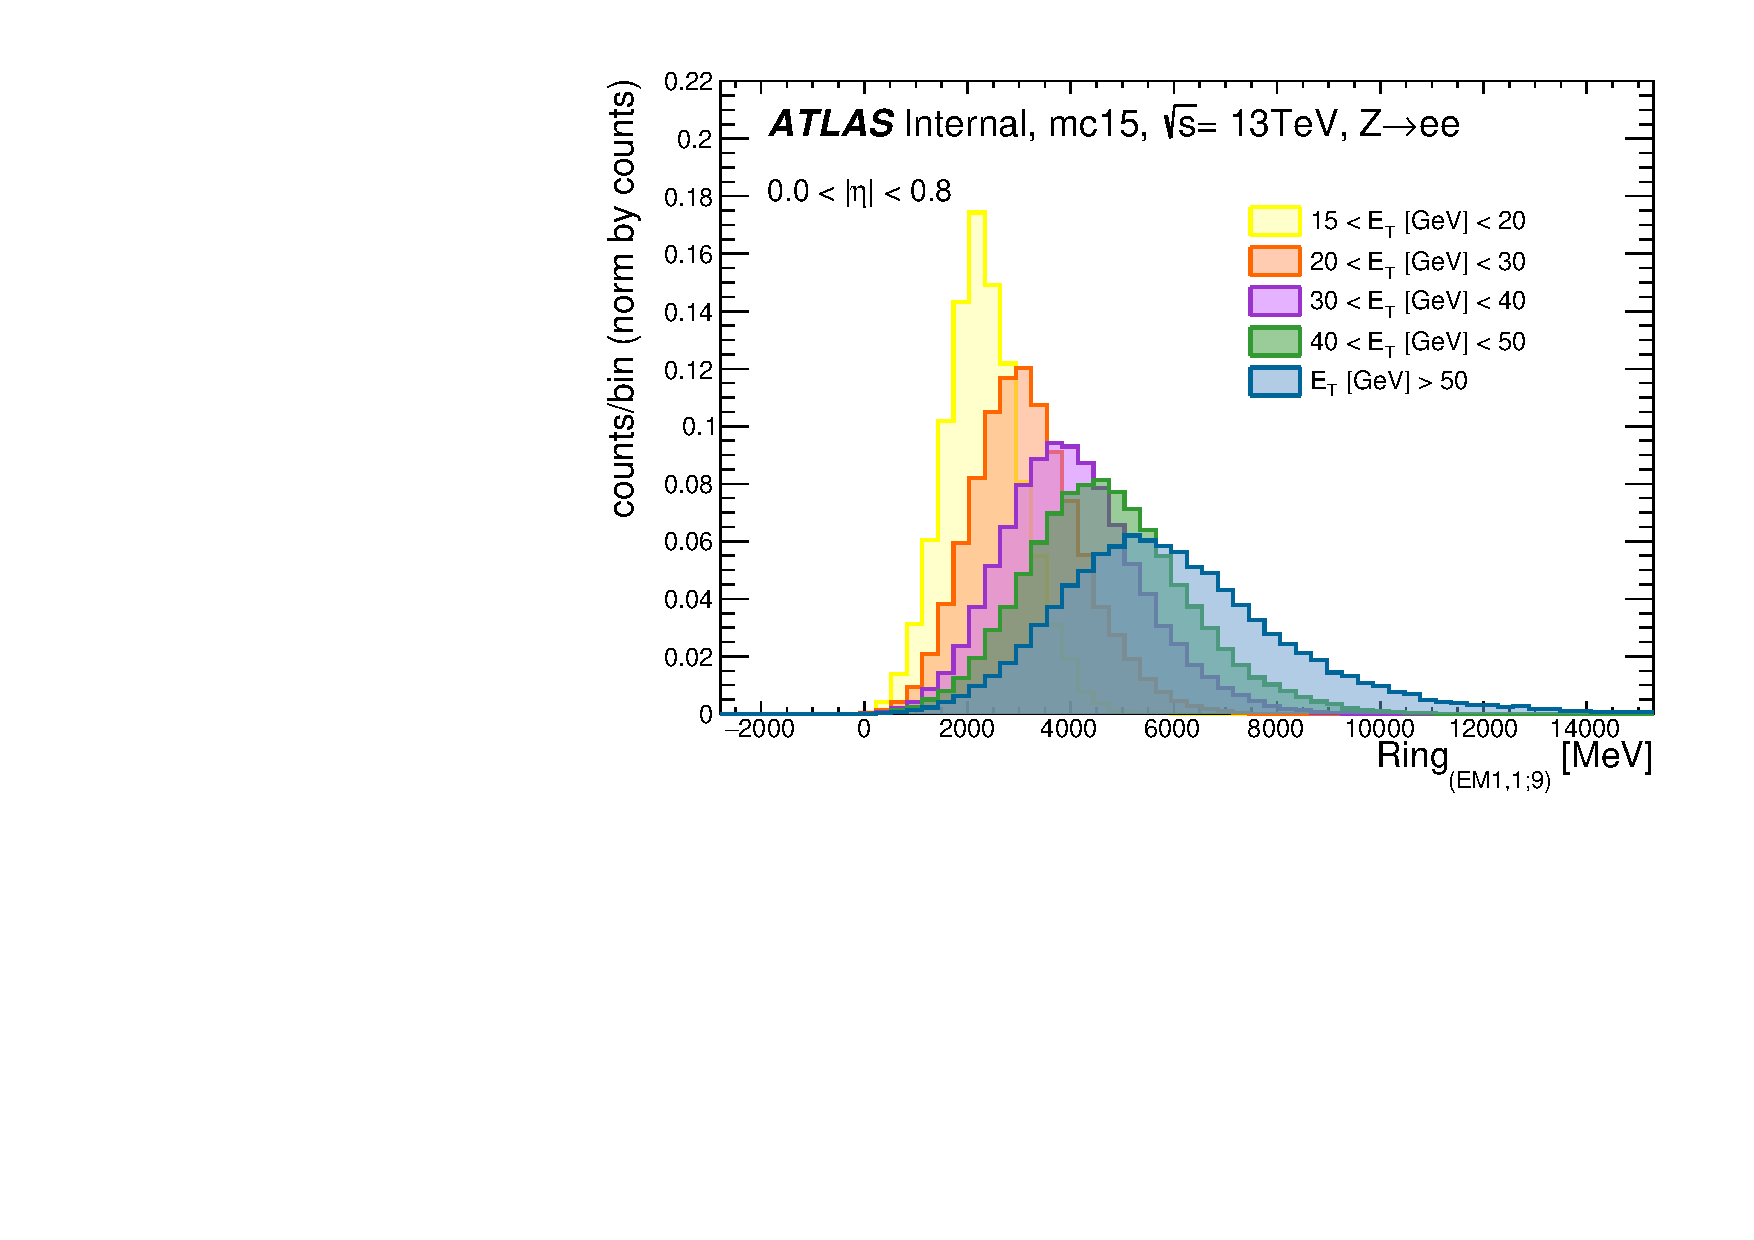
\includegraphics[width=\textwidth]{sections/03_ringer/figures/L2Calo_ring_9_eta0_etComp.pdf}
\centering
\caption{}%
\end{subfigure} \\
\begin{subfigure}[c]{.6\textwidth}
\centering
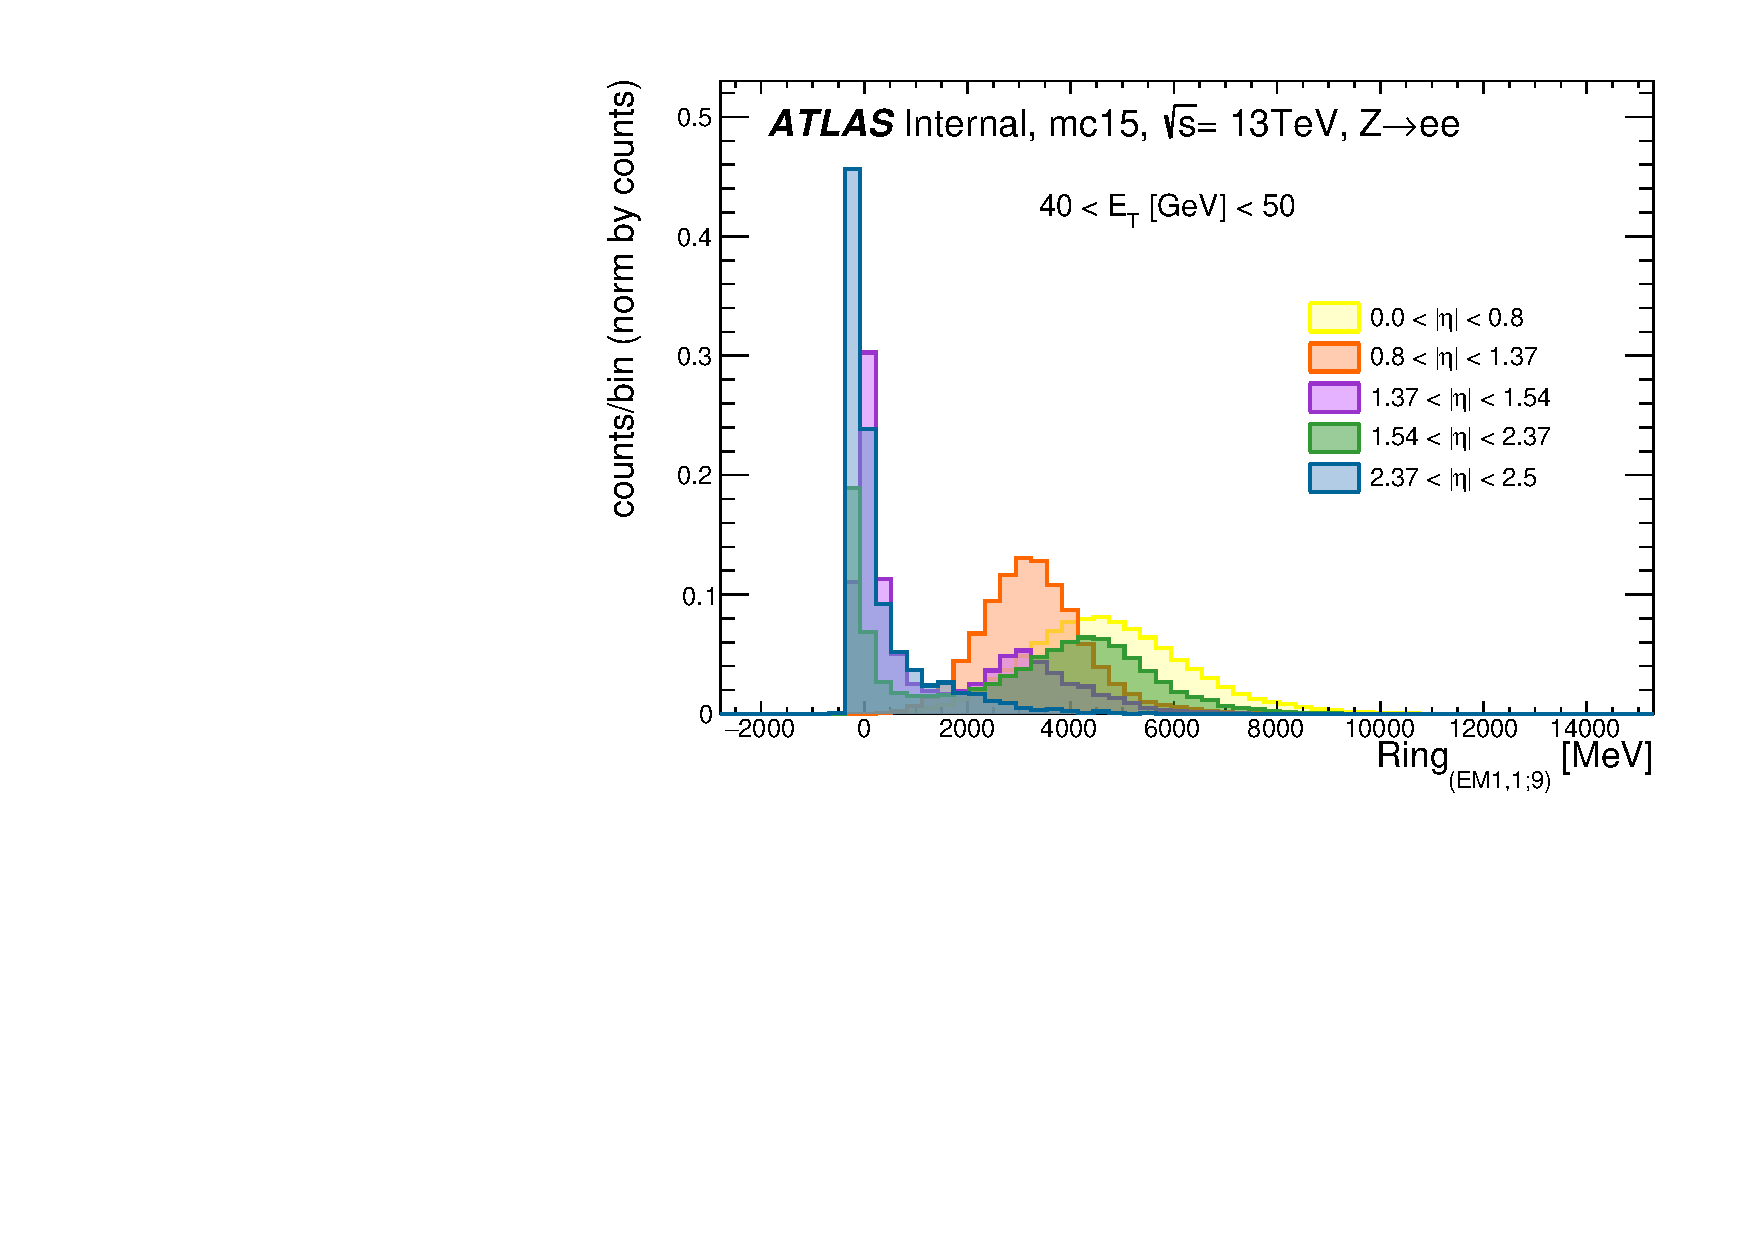
\includegraphics[width=\textwidth]{sections/03_ringer/figures/L2Calo_ring_9_et3_etaComp.pdf}
\caption{}%
\end{subfigure} 

\caption{Marginal distributions of the non-normalized first ring (hottest cell)
in the EM1 for the \et (a) and  \abseta (b) in Z$\rightarrow$ee simulated data
for the boundaries employed for extracting the \rnn{} discriminants in 2017.}%
%\label{fig:ring_distortion}
\end{figure}
\end{comment} 

In physics, such ensemble approach is consistent with the unfolding
strategy~\cite{unfolding_book}, usually employed for correcting for
measurement distortions due to the limitations of the instrumentation. It relies
on the definition of regions in variable space leading to these
variations where the detector efficiency, as well as other
sources of interference, are approximately constant. Once classification
efficiencies are evaluated using regions, it is natural that model parameters
are also defined for these regions. It is the case of the electron likelihood
algorithm~\cite{atlas_electron_id_offline}, which motivated the usage of
\eteta{} regions in the \rnn{} algorithm.

At the software level, the ensemble allows to handle all data in memory at once,
which speeds up the training cycle. Limiting the memory requirement for tuning
the models is particularly interesting in order to benefit from low-memory 
 processing nodes, which were predominantly available in 
WLCG~\cite{2015_lcg_tdr} during our
developments.\@ In addition, the decomposition of the problem can also lead to a
reduction of the training time~\cite{Polikar2006}, as observed heuristically\footnote{
  When using NVIDIA RTX 2080Ti in tensorflow 1.14 and a minibatch size of 1024, a 
  MLP with single hidden layer, we observed a substantial increase in the runtime (from 4 
  to 41 seconds per epoch) with respect to the ensemble version.} when
comparing the tuning time of the ensemble to a single and more complex model.
This effect can be related to the reduction of conflicting training information,
which can occur when a network is forced to learn several dissimilar functions
as distinct decision boundaries for each region~\cite{Auda1999,haykin_2008}.
Regarding the operation, the proposed ensemble only requires the choice of a
single model to operate instead of a more often committee machine approaches
that require the computation of different models in parallel with a fusion
method~\cite{zhou_ensemble}.  Therefore, the chosen ensemble configuration adds
minimal overhead in terms of trigger latency. Similarly, the choice was to
operate with low-complexity models, a single hidden layer with few neurons, to obtain a competitive method with respect to the cut-based
approach, in terms of processing speed.



\section{Training and Decision Making}%
\label{sec:tuning}

In this section, we detail the training and decision making tuning procedures
of the \rnn ensemble. Accordingly, we start (Section~\ref{ssec:fom}) with a
description of figures of merit that were employed.

The 2017 procedure (Section~\ref{ssec:2017}) derived the MLP ensemble
models with simulated data and defined the discriminant cut using
2016 collision data, targeting small signal efficiency discrepancy to triggering 
with cut-based trigger. The training procedure derived one ensemble of 25 MLP models for each one of the four\footnote{The working points are defined as: tight, medium, loose and very-loose.} working points. The ensemble boundaries are defined by Table~\ref{tab:ensemble_regions}. On the other hand, the 2018 training procedure (Section~\ref{ssec:2018})
employed a single ensemble structure for all working points and used
collision data for training, as it was the case for the derivation of offline
and final \hlt likelihood models~\cite{aaboud2019electron}.
% (since 2017~\cite{DAQ-2018-182})




\begin{comment}
\begin{table}[htb]
	\begin{center}
		{\small
			\begin{tabular}{cccc}
				\hline \hline
				\multicolumn{4}{c}{Model Adjust} \\ \hline \hline
				\multicolumn{4}{c}{$E_{T}$ {[}GeV{]} Boundaries} \\ \hline
				\multicolumn{4}{c}{$15 \leq E_T < 20 $}  \\
				\multicolumn{4}{c}{$20 \leq E_T < 30$}  \\
				\multicolumn{4}{c}{$30 \leq E_T < 40$} \\
				\multicolumn{4}{c}{$40 \leq E_T < 50$} \\
				\multicolumn{4}{c}{$50 \leq E_T < \infty$} \\\hline
				\multicolumn{4}{c}{$|\eta|$ Boundaries} \\ \hline
				\multicolumn{4}{c}{$0,0 \leq |\eta| < 0,8 $}  \\
				\multicolumn{4}{c}{$0,8 \leq |\eta| < 1,37$}  \\
				\multicolumn{4}{c}{$1,37 \leq |\eta| < 1,54$} \\
				\multicolumn{4}{c}{$1,54 \leq |\eta| < 2,37$} \\ 
				\multicolumn{4}{c}{$2,37 \leq |\eta| < 2,47$} \\ 
				\hline
				\hline
			\end{tabular}
		}
	\end{center}
	\caption{$E_T$ and $\eta$ boundaries used to create the ensemble.}
\end{table}

\end{comment}



\begin{table}[htb]
\begin{center}
	{\small
	\begin{tabular}{cccc}
		\hline \hline
		\multicolumn{4}{c}{Model Adjust}                                                                 \\ \hline
		\multicolumn{2}{c|}{$E_T$ {[}GeV{]} Boundaries} & \multicolumn{2}{l}{$|\eta|$ Boundaries}        \\ \hline
		\multicolumn{2}{c|}{$15 \leq E_T < 20 $}        & \multicolumn{2}{l}{$0.00 \leq |\eta| < 0.80 $}   \\
		\multicolumn{2}{c|}{$20 \leq E_T < 30 $}        & \multicolumn{2}{l}{$0.80 \leq |\eta| < 1.37 $}  \\
		\multicolumn{2}{c|}{$30 \leq E_T < 40 $}        & \multicolumn{2}{l}{$1.37 \leq |\eta| < 1.54 $} \\
		\multicolumn{2}{c|}{$40 \leq E_T < 50 $}        & \multicolumn{2}{l}{$1.54 \leq |\eta| < 2.37 $} \\
		\multicolumn{2}{c|}{$50 \leq E_T < \infty $}    & \multicolumn{2}{l}{$2.37 \leq |\eta| < 2.47 $} \\ \hline \hline
	\end{tabular}
}
\end{center}
\caption{$E_T$ and $\eta$ boundaries used to create the ensemble.}
\label{tab:ensemble_regions}
\end{table}

\subsection{Figures of Merit}\label{ssec:fom}



The sets $\Theta_{\text{e}}$ and $\Theta_{\text{b}}$ of real and fake electrons, respectively, were selected by using the \tnp{} method and the offline selection for trigger developments (Section~\ref{ssec:dataset}). Let the existence of a model $\mathcal{C}$ representing a function $f_{\mathcal{C}} : \Theta \rightarrow \mathbb{R}$ optimized to perform the binary classification task. Here, $\mathbb{R}$ is the set of real numbers, as the neural network ensemble produces real numbers at the single output node for trigger decisions.  From supervised optimization, the model $\mathcal{C}$ outputs $\hat{H}:=f_{\mathcal{C}}(x)$ with target $H$ for a sample $x \in \Theta$. The operation of $\mathcal{C}$ results, respectively, in the selection of the subsets $\mathcal{O}_{\text{e}|\text{e}}$ and $\mathcal{O}_{\text{e}|\text{b}}$ from $\Theta_{\text{e}}$ and $\Theta_{\text{b}}$ as trigger candidate electrons in the \fastcalo{} processing step of the \hlt{} by defining the decision making procedure $\tau : \mathbb{R} \rightarrow \left\{\text{e},\text{b}\right\}$. As there is a single output node for each neural network in the proposed \rnn{} ensemble, $\tau$ corresponds to a mapping that is a decision threshold for selecting an electron candidate when the output node is above the given threshold.  


We explicitly define some convenient figures of merit in \tablename~\ref{tab:figures_of_merit}. It is possible to tune $\mathcal{C}$ to result in a proper working point, (i.e. a targeted value of \pd{} or \pf{}) by adjusting $\tau$. All possible working points of $\mathcal{C}$ are defined by the Receiver Operation Characteristic (ROC) curve~\cite{van_trees_part1}, but keeping fixed the electron detection probabilities, or signal efficiencies, with respect to the previous baseline cut-based trigger. The \spindex{}~\cite{dos2006neural} index, the square root of the product of the geometric and arithmetic averages of the efficiencies for the signal and background categories, collapses when efficiencies on either signal or background events decrease significantly. Thus, the SP index provides a unidimensional space that allows tuning $\mathcal{C}$ for obtaining high efficiency in a balanced manner for both classes, which is given by choosing the $\spmax{}:=\max(\spindex{})$ working point.





\begin{table}[hbt]\footnotesize
\centering
\caption{Names, symbols and definitions of the figures of merit employed. More
  than one symbol and names can be found in different fields for some figures.
  We will use the names indiscriminately throughout the text, however the
  symbols to be employed in the text are prefixed with a `$\rightarrow$' symbol.
  The unary operator $|\cdot|$ represents the cardinality of a
set.\label{tab:figures_of_merit}}
\resizebox{\textwidth}{!}{%
\begin{tabular}{cllc}
\hline
\hline
&  Symbol & Name & Definition \\
\hline
$\rightarrow$ & $\pd{}$ & Probability of detection &
\multirow{3}{*}{$\cfrac{|\mathcal{O}_{\text{e}|\text{e}}|}{|\Theta_{\text{e}}|}$}
\\
& \multirow{2}{*}{$\text{P}_{\text{e}|\text{e}}$} & Electron efficiency & \\
& & Signal Efficiency & \\
\hline
$\rightarrow$ & $\mathbf{\pf{}}$ & Probability of false alarm &
\multirow{3}{*}{$\cfrac{|\mathcal{O}_{\text{e}|\text{b}}|}{|\Theta_{\text{b}}|}$}
\\
& \multirow{2}{*}{$\text{P}_{\text{e}|\text{b}}$} & Fake rate & \\
& & Background efficiency & \\
\hline
& \spindex{} & Sum-product index & $\left(
  \left(\pd{}\cdot(1-\pf{})\right)^{\nicefrac{1}{2}} \cdot
  \left(\pd{}+(1-\pf{})\right) \cdot \nicefrac{1}{2}
  \right)^{\nicefrac{1}{2}}$ 
  \\
\hline
& MSE & Mean squared error & $\sum\limits_{x\in\Theta} \cfrac{\left(\hat{y} -
y\right)^2}{|\Theta|}$ \\
\hline
\hline
\end{tabular}
}
\end{table}











\subsection{Training Procedure For 2017 Data}\label{ssec:2017}

The training procedure and decision making processes are the same for all phase
space regions and a summary of the process is provided in
\tablename~\ref{tab:2017_ringer}. For the \rnn{}, $\mathcal{C}$ is an ensemble of
MLPs and each MLP is an expert model for a single phase space
region, containing its own topology and parameters.

The model parameters have been optimized using events selected on simulation datasets
(Section~\ref{ssec:dataset}). The structure is a fully-connected single
hidden layer, which may contain from 5 to 20 hidden units, an input layer with 100 inputs, one for each ring, and an output layer with a single neuron. The activation
functions for both hidden and output neurons are the hyperbolic tangent, which has been often used in MLP designs~\cite{haykin_2008}. 

To assess the statistical fluctuations of the efficiency measurements, the stratified k-fold ($k=10$) cross-validation method~\cite{haykin_2008} was used at the price of increased computational cost by repeating training and testing procedures on different
randomly chosen subsets. The stratified k-fold is
among the most common cross-validation techniques and consists of partitioning
the dataset in k disjoint subsets, each model tested with the $i$th subset and
trained with the remaining ones. The dataset stratification follows the
empirical order of the event selection, in order to allow straightforward job
parallelization, i.e.\ random permutation is not employed. The possible effect
of a temporal structure in data was neglected as 2017 training procedure
employed simulation data.

In case of similar cross-validation efficiencies when comparing standard
error confidence interval corresponding to \SI{68}{\%} for different
configurations, the choice is based on
parsimony~\cite{haykin_2008, medeiros2001statistical} so that the structure with lower number of hidden units
is employed as higher generalization power can be expected. 





\begin{table}[ht!]\footnotesize
\centering
\caption{Summary of the tuning procedure and decision making strategies employed
to obtain the \rnn for 2017 operation. See text for more
details.}\label{tab:2017_ringer}
\resizebox{\textwidth}{!}{%
\begin{tabular}{p{6cm}p{10cm}}
\hline
\hline
\hline
Criterion & Value \\
\hline
\hline
\multicolumn{2}{c}{Ensemble Composition} \\
\hline
\hline
Model & Fully connected MLP, 1 hidden-layer ($\tanh(.)$) and 1 output ($\tanh(.)$) \\
Phase space bins for Model Tuning &
See Table~\ref{tab:ensemble_regions} \\
%See Tables~\ref{tab:comp_etabins} and \ref{tab:comp_etbins} \\
\hline
\hline
\multicolumn{2}{c}{MLP Training} \\
\hline
\hline
Core Framework & \emph{FastNet} (~\cite{tuningtools}) \\
Dataset and event selection & Simulation (Section~\ref{ssec:dataset})\\
Input Features & Concentric ring sums of energy around the particle axis  \\
Normalization & Absolute of the total ring energies (Section~\ref{top:pp}) \\
Cost-function for tuning & MSE \\
Back-propagation method & RPROP (default parameters, except $\eta^+=1.1$) \\
Targets (Electron/Background) & +1/-1 \\
Batch size & Number of observations in the smaller class \\
Maximum number of training epochs & $\infty$ \\

Over-training evaluation & Multi-stop (see text) using
50 epochs stop criterion \\

Working point reference & Baseline chain efficiencies at \hltcalo \\

Evaluated structures & Number of hidden units ranging from 5 to 20 units \\

Initializations & 100 (Nguyen-Widrow method) \\

Cross-validation method & Stratified k-fold ($k=10$, validation set used for
both testing and early stop computation) \\

Cross-validation subset retrieval method & Split data uniformly into k subsets,
random permutation not applied. Remaining samples are put one by one into the
first subsets \\
ROC extraction method & 1,000 linearly spaced points between model targets \\
\hline
\hline
\multicolumn{2}{c}{Training Evaluation and Operating Model Selection } \\
\hline
\hline

Working Point & ROC point closest to signal efficiency reference and \spmax{}
value \\

Best Initialization Choice & Lowest fake rate (validation set) when operating in
a region of up to $\epsilon=0,2~\%$ of the reference signal efficiency \\

Model Topology Selection & Graphical analysis using box plots \\

Operating Model Choice & Lowest fake rate (using full stats.) when operating in
a region of up to $\epsilon=0,2~\%$ of the reference signal efficiency \\

Operation Extrapolation & Yes, eventual observations outside model phase
space regions use the nearest expert model (in lowest Euclidean
distance in $\et\times\eta$ axis) \\

\hline
\hline
\multicolumn{2}{c}{Decision Making} \\
\hline
\hline

Pile-up Efficiency Correction & Compute straight-line balancing efficiency within
$\avgmu=[0,20,40]$ avg.\@ collisions \\
Dataset and event selection & 2016 $13\;\text{TeV}$ p-p collision data
(GRL: v88), except for reprocessing reference run \\
Decision Making Strategy & Linear fit to the network output without applying the
transfer function w.r.t. $\avgmu$ up to 40$\;$avg.\@ collisions.
When $\avgmu>40$, set $\avgmu = 40$ (2016 upper bound) \\
%Cross-Validation Method & None \\

Phase space bins for Linear Fit & See
Table~\ref{tab:ensemble_regions}\\
%Tables~\ref{tab:comp_etabins} and~\ref{tab:comp_etbins} \\
Target Working Point & Keep HLT signal efficiency of the proposed chain as near
as possible from the respective baseline chain \\
\hline
\hline
\hline
\end{tabular}
}
\end{table}





For each cross-validation sort and working point, 100 networks, initiated
as from~\cite{initnw}, are optimized by back-propagating MSE through the RPROP
algorithm~\cite{rprop} with all parameters set to default,
except for the parameter that regards the multiplication factor of the weight update rate when gradient direction remains the same as of the previous iteration. It was 
%except for
%$\eta^+=1.1$ (default is 1.2). This particular
%parameter regards the multiplication factor of the weight update rate when
%gradient direction remains the same as of the previous iteration. It was
observed during Run~1 that this modification improved convergence speed. RPROP
is an adaptive gradient descendent technique that is resilient to the size of
the derivatives. This repeated model initialization aims at
avoiding poor sub-optimal solutions due to usage of gradient-based algorithms as
RPROP in optimisation problems involving non-convex and complex function.
For each training procedure, only three models out of the 100 are retained: two
for retrieving the best efficiency when fixing the \pd{} or \pf{} to the
baseline \fastcalo{} efficiency and another resulting in the \spmax{} value.
Early stopping~\cite{haykin_2008} is employed to avoid model over-training. The
selection of the optimal iteration and operating model is based on an heuristic approach (multi-stop)~\cite{Goodfellow2016}.


Computational resources from the WLCG and \emph{Lobo Carneiro}
super-cluster~\cite{lobo_carneiro} were used to tune 1.3~M shallow-learning
neural networks, which resulted in an ensemble of \SI{20}{MLPs} (five in \et{}
$\times$ four in \abseta{}) for each one of the four working points used by
electron chains in the HLT (see Section~\ref{ssec:egamma_trigger}).
Here, the first training strategy considered only four regions in $|\eta|$ ($0.0\rightarrow 0.8\rightarrow1.37\rightarrow2.5$).
Except for few exceptions, the models in the ensemble employed 5 neurons in the 
hidden layer.  Thus, for 2017 operation, 
\rnn{} operation did not result on
successive contained sets for more stringent working points, i.e. an electron
candidate accepted by \medium{} is not necessarily also accepted by \loose{}
working point. %To the best of our knowledge, this does not impact the \hlt{}
%given that triggers are employed in parallel both for operation and analysis.
%Thus, eventual disagreements between their selections are irrelevant.


After the training stage, the decision is taken by applying a threshold in the
one-dimensional output node of each expert MLP.\@ 
Inspired by the HLT likelihood algorithm, the threshold applied for
\rnn is also computed as a linear function of \avgmu{}.
However, when employing the standard NN parametrisation, a non-linear
behavior was observed near the asymptote of the output activation 
function (See Figure~\ref{fig:nn_correction_with_tansig}), which occured
for the medium and tight operation points. Heuristically, it was 
observed that this behaviour can be avoid when replacing the output
activation by a linear function (Figure~\ref{fig:nn_correction_without_tansig})
for operation, after the training stage is completed.
This strategy provides a linear
behavior of the targeted signal efficiency with respect to the online pile-up
estimator. Except for the end-cap region during 2017, the boundaries for
defining discriminant requirement parameters were the same as those employed in
the \rnn ensemble (Section~\ref{top:nn_ensemble}). The 
interpolation for the \et{} values, which was employed in the likelihood as a smoothening strategy~\cite{aaboud2019electron}, was
%interpolation in
%\et{} employed in the likelihood as a smoothening
%strategy~\cite{aaboud2019electron} was 
not used (Section~\ref{ssec:egamma_trigger}).
%Tables~\ref{tab:comp_etabins}
%and~\ref{tab:comp_etbins} show the boundaries in the \eteta{} axis used for
%Run~2 operation.



\begin{figure}[h!tb]
  \begin{center}
  %\hspace{0.01\textwidth}
  \begin{subfigure}[c]{.48\textwidth}
  \centering
  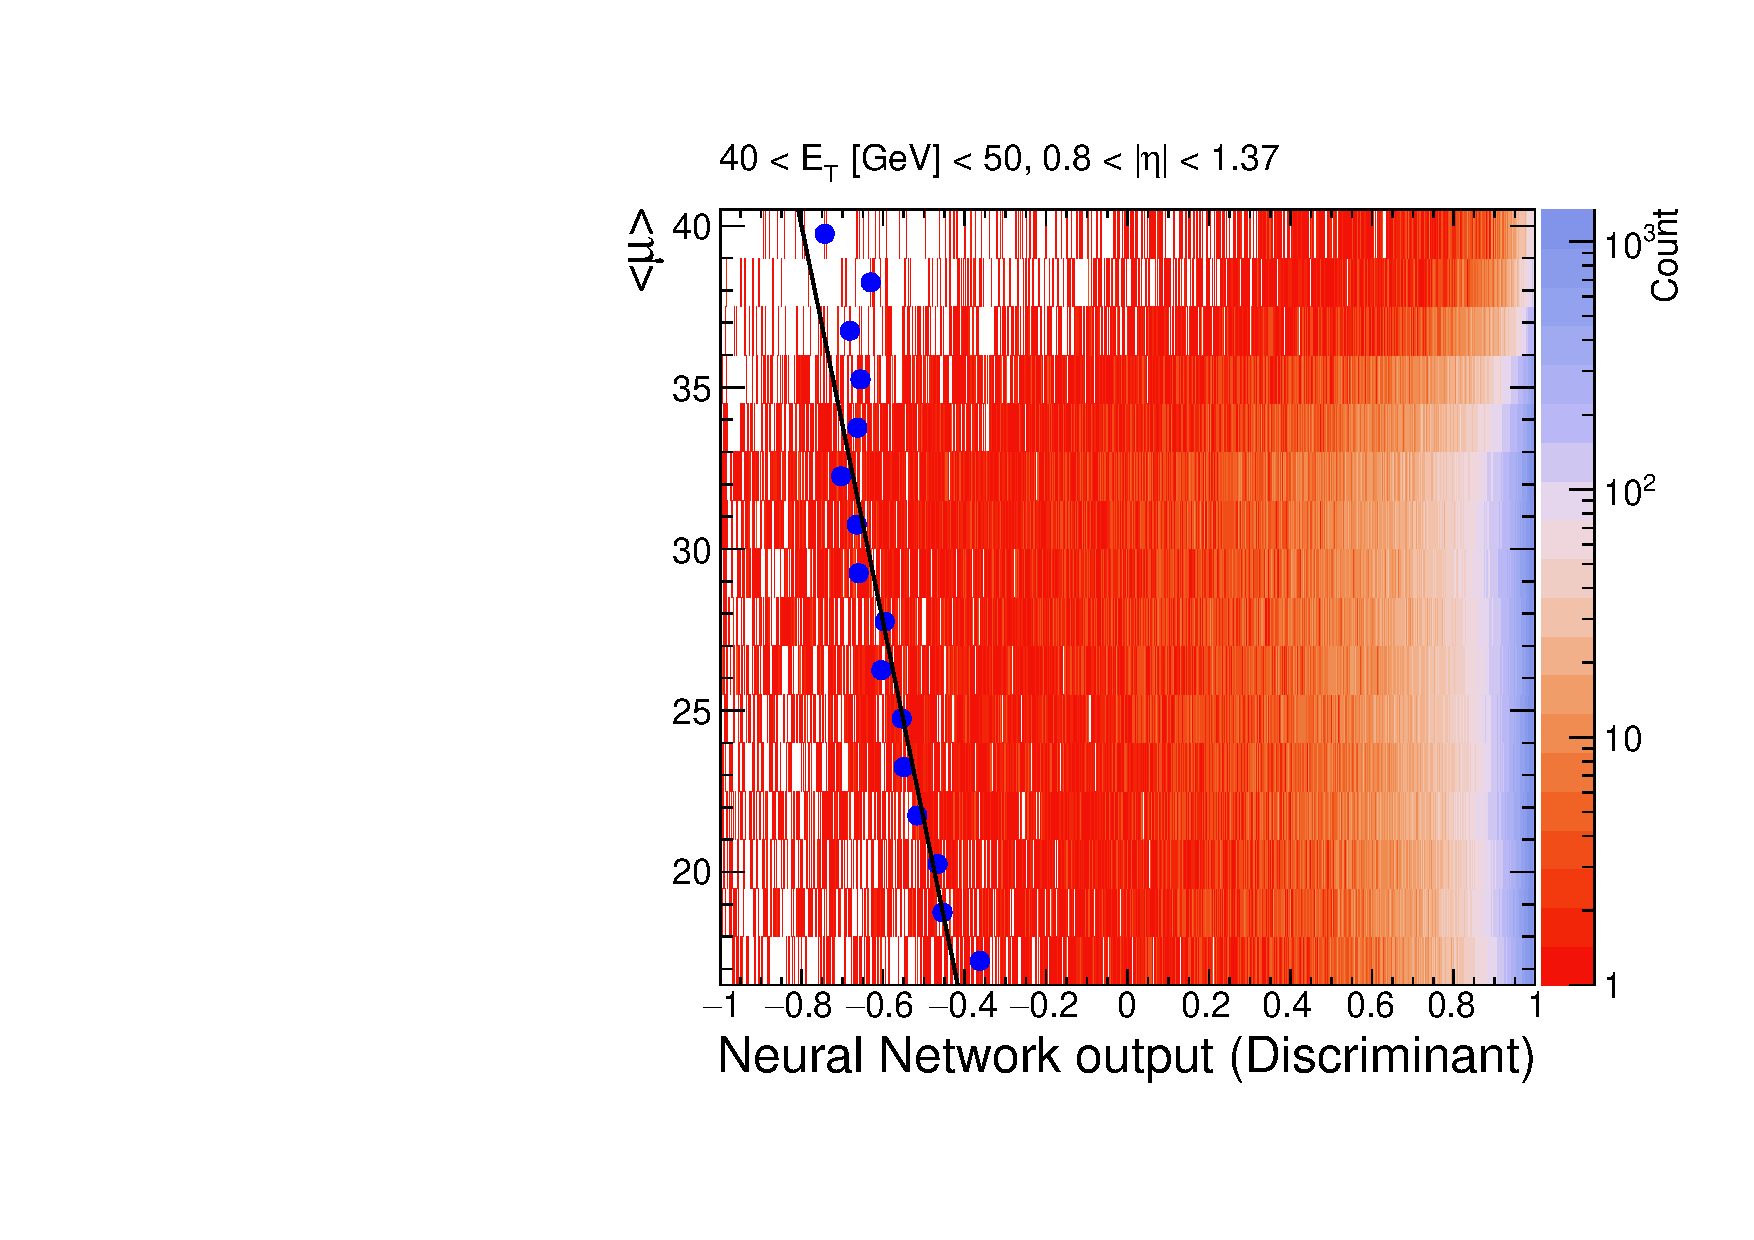
\includegraphics[width=\textwidth]{sections/03_ringer/figures/th2_signal_tight_cutbased_et3_eta1_with_tansig.pdf}
  \caption{Neural output with hyperbolic tangent w.r.t pileup.}
  \label{fig:nn_correction_with_tansig}
  \end{subfigure}
  \hfill
  \begin{subfigure}[c]{.48\textwidth}
  \centering
  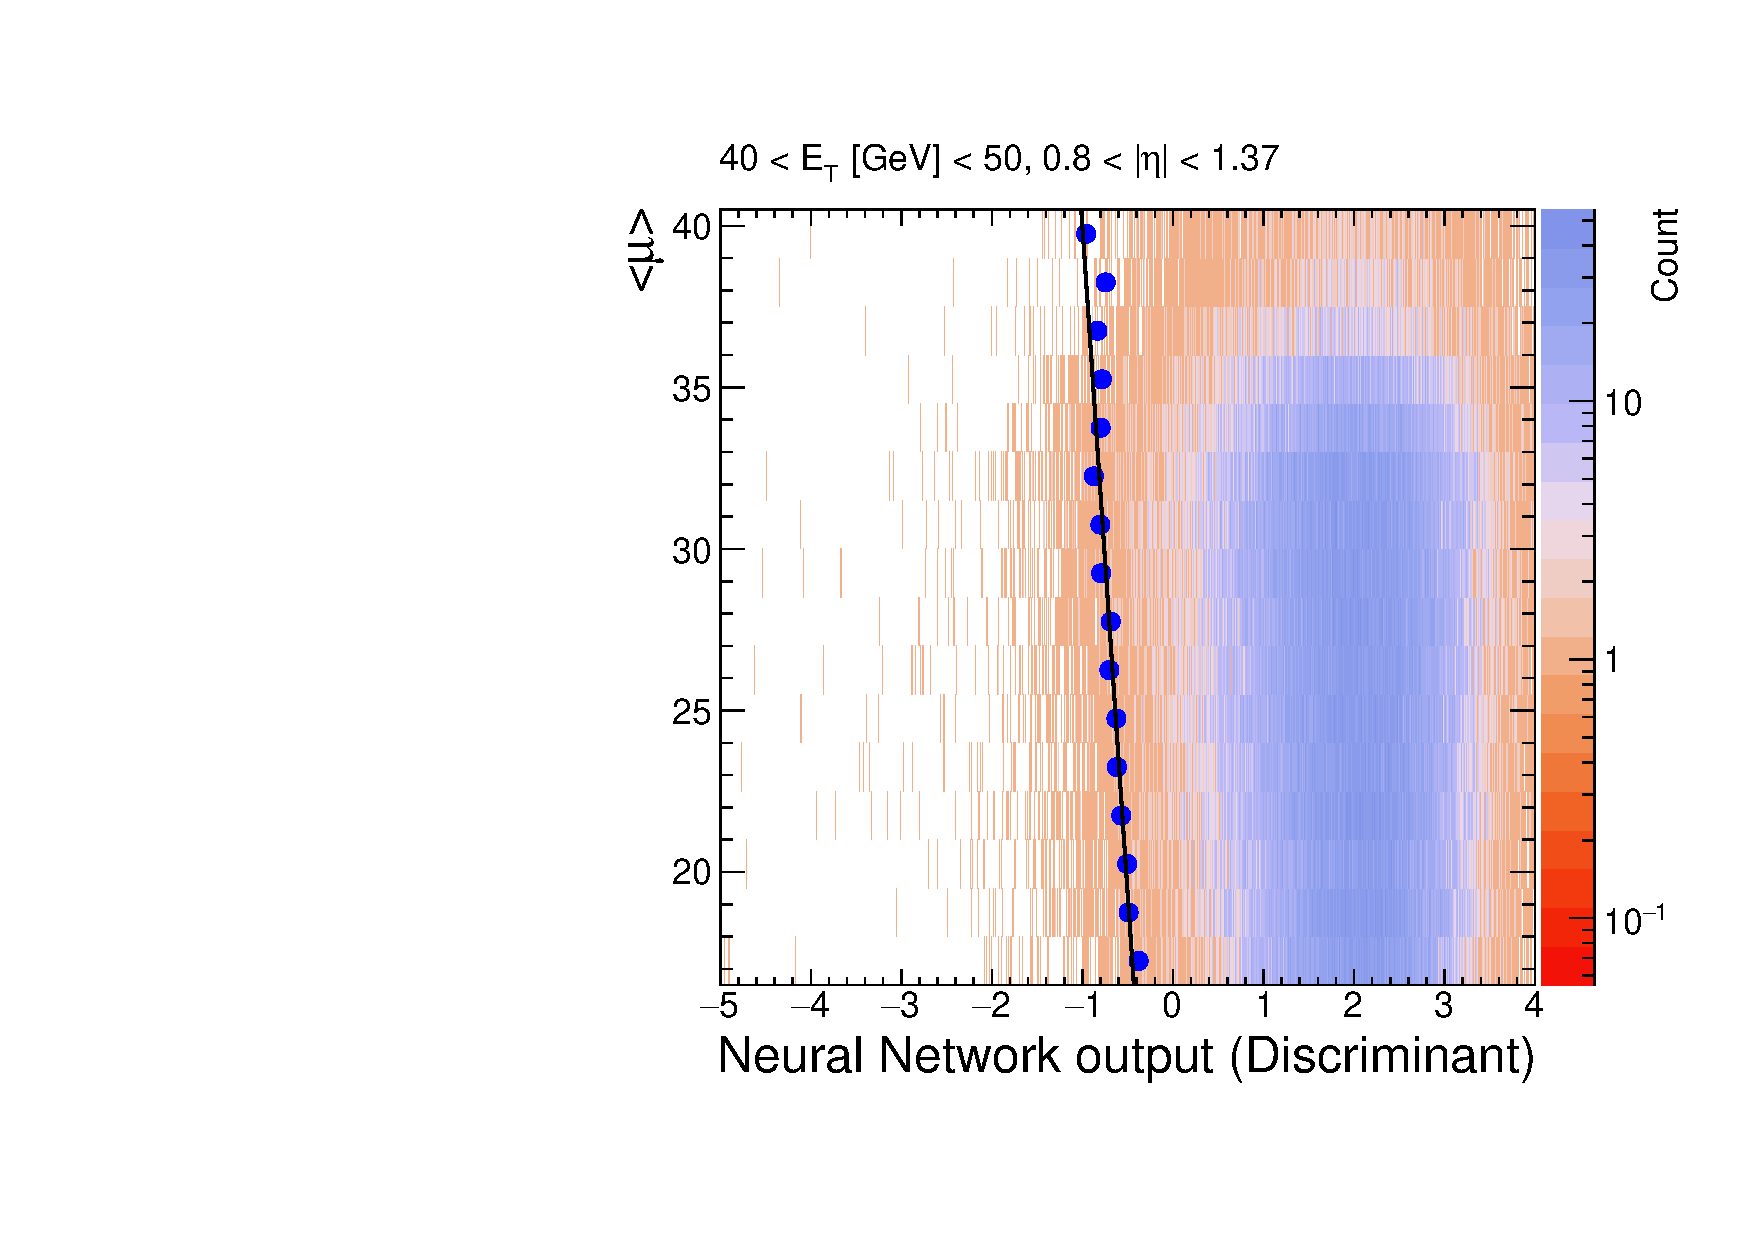
\includegraphics[width=\textwidth]{sections/03_ringer/figures/th2_signal_tight_cutbased_et3_eta1_without_tansig.pdf}
  \caption{Neural output with linear activation w.r.t pileup.}
  \label{fig:nn_correction_without_tansig}
  \end{subfigure}
  %\hfill
  \caption{
    \rnn output as a function of \avgmu{} for $Z\rightarrow ee$ probes in 
    2016 collision data.
    The computed threshold per \avgmu{} unit for achieving the target 
    efficiency is shown in blue full circle. The black line is a linear fit of the thresholds.
    The output space is computed using the trained model without modifications 
    in (a), while in (b) the output activation is replaced by the identity.
    The electron probes are selected using the training criteria.
  }%
  \end{center}
  \end{figure}




%
\begin{table*}[htb]
\caption{Boundaries in absolute electron pseudorapidity used to define the bins
  of the ensemble. The term `MLP' refers to the boundaries for the operation of
  the \rnn{} specialist network and with the `discriminant' term we define the
  boundaries for defining the thresholds for each requirement. Here, \emph{both}
refers to the computation of either the model parameters or the discriminant
respecting the same boundaries.}%
\label{tab:comp_etabins}
\begin{center}
\begin{tabular}{lcccccc}
\hline
\multicolumn{7}{c}{2017 \rnn  bin boundaries in \abseta}\\
\hline
MLP & 0.0 & 0.8& 1.37& 1.54& & 2.5 \\
Discriminant & 0.0& 0.8& 1.37& 1.54& 2.37 & 2.5 \\
\hline
\multicolumn{7}{c}{2018 \rnn  bin boundaries in \abseta}\\
\hline
Both & 0.0 & 0.8& 1.37& 1.52& 2.37 & 2.47 \\
\hline
\end{tabular}
\end{center}
\end{table*}



%


\begin{table*}[htb]
\caption{Boundaries in electron transverse energy defining the specialist
  network and discriminant threshold values to be employed by the \rnn{}
  algorithm.
}%
\label{tab:comp_etbins}
\begin{center}
\begin{tabular}{cccccc}
\hline
\multicolumn{6}{c}{2017 and 2018 \rnn bin boundaries in \Et [\GeV]}\\
\hline
15& 20& 30& 40& 50 & $\infty$ \\
\hline
\end{tabular}
\end{center}
\end{table*}






% TODO A plot showing the particular impact in the 2.37 region
% TODO Cross-validation: error bars
% TODO MLP training example
\begin{figure}[h!t]
\centering
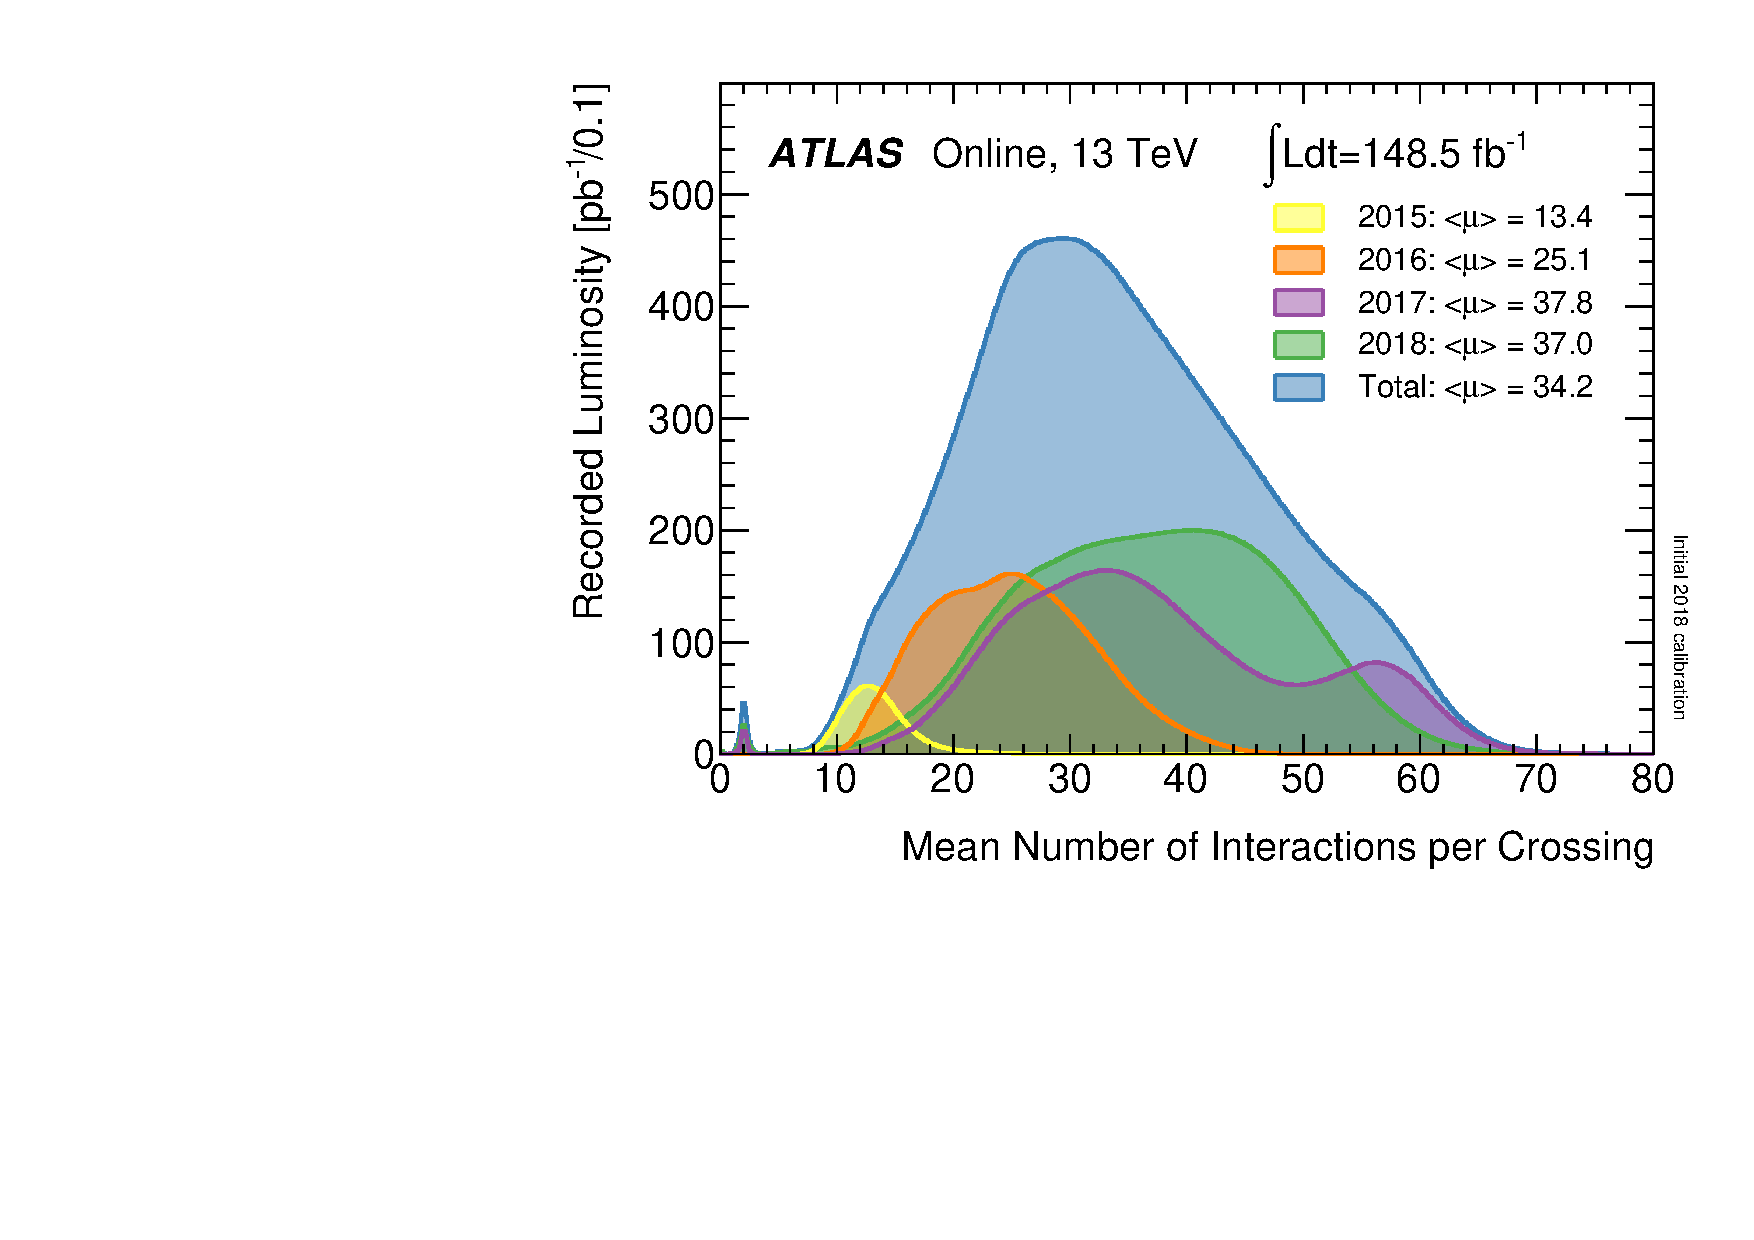
\includegraphics[width=0.6\textwidth]{sections/03_ringer/figures/mu_2015_2018.pdf}
\caption{\label{fig:mu_2015_2018}
Luminosity-weighted distribution of the mean number of interactions per crossing
for the Run~2 pp collision data at 13 TeV centre-of-mass
energy.~\cite{atlas_lumi_run2_results}}
\end{figure}


The linear correction applied during 2017 is upper-bounded by $\avgmu=40$
collisions, a quantile encompassing a large fraction of 2016 data
(Figure~\ref{fig:mu_2015_2018}). The objective was to avoid extrapolation to a
regime not previously evaluated, which could lead to unexpected growth in the
background rate and, thus, to data-taking issues due to the large CPU demand
from the electron triggers.

% (decision taking)
To account for Monte Carlo data mis-modeling, the parameters of the linear threshold
correction were derived using 2016 collision data. Furthermore, it was observed
that the rings in the region $2.37<\abseta<2.47$ had particular profiles due to
the lack of strip cells in this region and demanded a specific discriminant requirement in order to keep signal efficiencies near triggers without the \rnn{}. In order to avoid retraining all models, it was decided to split the last $|\eta|$ region in two, from $1.37\rightarrow 2.5$ to $1.37\rightarrow2.37\rightarrow2.5$, and duplicate all models, for this region, to the new bin. Finally, the ensemble used to operates in 2017 has a total of 25 MLP models.



%It drastically affected the ring profiles in this region which resulted in a shift
%of the signal discriminant towards the direction of the background target and
%demanded a specific discriminant requirement in order to keep signal
%efficiencies near triggers without \rnn{}.

\FloatBarrier
\subsection{Training Procedure For 2018 Data}\label{ssec:2018}

Most of the procedure was kept unchanged for 2018, with modifications shown in
Table~\ref{tab:2018_ringer}.
In opposition to 2017, the developments for 2018
could benefit from collision data 
representing similar data taking conditions.
%In 2018, the developments could benefit from collision data representing similar conditions to data taking. 
The major alteration in 2018 tunes was the derivation of the \rnn{} ensemble with collision data based on \Zee{} \tnp{} event selection, in order to avoid the Monte Carlo data mis-modeling.

We also simplified the training strategy by abandoning the selection of three
models for each training and keeping only the \spmax{} model as the previous approach was more complex without a clear
payoff in trigger efficiency.
Likewise, MLPs with 5 to 10 units in the hidden layer were tuned, as most models did not require
more than 10 units in 2017. With a larger time span for entering operation, we
added MLPs specialized in the region where we detected a change in the ring
profiles before 2017 operation between $2.37<\abseta<2.47$, resulting in the operation of
\SI{25}{MLPs}. The correction limit was set to
$\avgmu{}=100$~collisions or, in other words, removed for 2018 operation, given
that the data-taking 
conditions never reached such a large pileup level. By
%conditions did not extrapolate this value. By 
assuming a linear efficiency extrapolation,%\footnote{It is worth noticing that the linear
%fit is reasonably good for the Run~2 conditions.}
it was observed that most phase space regions did not reach background efficiencies
larger than \SI{15}{\%} before arriving at $\avgmu=100$~collisions, while same
signal efficiencies were maintained.

% NOTE TriggerEgammaMeeting_20180213

% NOTE TriggerEgammaMeeting_20180213

\begin{table}[ht!]\footnotesize
\centering
\caption{Changes in the derivation of the 2018 \rnn operation models with
respect to 2017 models. See text for more details.}\label{tab:2018_ringer}
\resizebox{\textwidth}{!}{%
\begin{tabular}{p{6cm}p{10cm}}
\hline
\hline
\hline
Criterion & Value \\
\hline
\hline
\multicolumn{2}{c}{Ensemble Composition} \\
\hline
\hline
Phase space bins for Model Tuning &
Added one new boundary for the tunes in \eta, see Table~\ref{tab:ensemble_regions} \\
\\
\hline
\hline
\multicolumn{2}{c}{MLP Training} \\
\hline
\hline

Dataset and event selection & 2017 $13$ TeV $p-p$ collision data (Section~\ref{ssec:dataset})
\\ 
Over-training evaluation & Stop when fail to improve \spmax for 50 epochs
(compute ROC at each epoch) \\

Evaluated topologies & Hidden layer with number of neurons ranging from 5 to 10
units \\

\hline
\hline

Fit Method & Linear fit method
$\chi^2=\frac{{(y-f(x))}^2}{e_y^2+{(0,5{(e_{xl}+e_{xh})}f\prime(x))}^2}$ 
where $f(x)$ is the function to be fitted, in this case an affine function; and $y$ is the lower (upper) error of the ordinates if $f(x)$ is below (above) $y$, and $e_{xl}$ ($e_{xh}$) is the lower (upper) error on the abscissas. \\

Dataset and event selection & 2017 $13\;\text{TeV}$ p-p collision data (GRL:
v97), except for reprocessing reference run \\

Decision Making Strategy & Linear fit of the network output by replacing the transfer function w.r.t. $\avgmu$ up to 100$\;$avg.\@ collisions.
When $\avgmu >100$, set $\avgmu = 100$ \\

\hline
\hline
\hline
\end{tabular}
}
\end{table}







 % need to fix table and alg
\chapter{Online Deployment}%
\label{sec:operation}



This section reports the \rnn{} operation in both 2017
(Section~\ref{ssec:2017_ringer_operation}) and 2018
(Section~\ref{ssec:2018_ringer_operation}) data acquisition periods. The operation efficiencies
are computed with respect to offline electrons, as indicated in
Section~\ref{ssec:dataset}\footnote{For efficiency measurements in this section,
	fake electrons are selected always employing \veto\vloose{} offline likelihood
	working point.}. Firstly, the detail of the algorithm cycle used during Run~2
(Section~\ref{ssec:run2_rnn_cycle}) is presented.

\section{Run~2 \rnn{} Cycle}\label{ssec:run2_rnn_cycle}

During the Run 2, the actual \rnn{} implementation
%The \rnn cycle 
can be partitioned into four chronological stages:

\begin{enumerate}[i]
  \item A development stage up to early 2017, where the \rnn{}
      potential was estimated from trigger emulation and data reprocessing;
  \item The commissioning stage (\SI{5.4}{\per\femto\barn}) occurred in
      early 2017 runs, where all primary
      triggers were duplicated with either the \rnn{} or cut-based algorithms
      operating in the \fastcalo{} stage of the HLT;
  \item The operation of the method as the baseline trigger, which occurred after 2017 Technical Stop 1 (TS1). For
    monitoring purposes, and to allow precise statistical evaluation of eventual
    disagreements between the \fastcalo{} methods from an offline
    perspective (Section~\ref{sec:off_ana}), a duplicated trigger pair, i.e.
    with and without \rnn{}, was kept operating unprescaled during this period
    (\SI{39.0}{\per\femto\barn}). Here, the efficiencies of the
    duplicated triggers in 2017 (Section~\ref{ssec:2017_ringer_operation}) are compared;
  \item Finally, the duplicated trigger was removed for 2018 operation.
    Therefore, the evaluation of 2018 \rnn{} operation relying on a comparison with
    2017 efficiency is presented in Section~\ref{ssec:2018_ringer_operation}.
\end{enumerate}

\section{2017 Operation}\label{ssec:2017_ringer_operation}

% FIXME Don't forget that there are some of these plots that were already
% approved.

%A backup trigger ($\text{e28\_lhtight\_nod0\_ivarloose}$) was employed for
A backup $E_T > 28$ GeV isolated trigger with Tight selection and without the \rnn{} was employed for
monitoring purposes after the first technical stop (TS1). During the monitoring process, a similar
operation of both triggers was observed in terms of signal efficiency using the
integrated luminosity along the period, as shown in
Figure~\ref{fig:e28_triggers}. The trigger
turn-on curves exhibit similar profile. In $\eta$, \rnn{} shows a reasonably symmetric
profile with respect to positive and negative $\eta$. In addition, a difference of about half to one percentage point may be observed in $\eta$ because of the transition region between the endcap and barrel. Besides
aforementioned points, overall efficiency fluctuations are smaller than a few
per-mille. Although a slightly more prominent efficiency loss with respect to
\avgmu{} is observed in Figure~\ref{fig:e28_comp_mu} for the \rnn{} trigger, the
electron efficiency was kept nearly the same. Such loss occurs after the
linear threshold correction limit of $\avgmu=40$ that was employed during 2017.

Other important triggers were assessed by comparing the trigger efficiencies on
2017 data collected before and after switching to the \rnn{} algorithms.  As it can be observed in Figure~\ref{fig:2017_ts1}, the electron efficiency was also kept nearly unchanged for relevant single electron triggers. Note that results in
this plot are computed with two different data taking periods: with or
without the \rnn{} algorithm. %The loosest likelihood trigger with 17 GeV energy threshold shows the efficiency in the lowest-energy-threshold 




\begin{figure}[h!tb]
  \begin{center}
  \begin{subfigure}[c]{.59\textwidth}
  \centering
  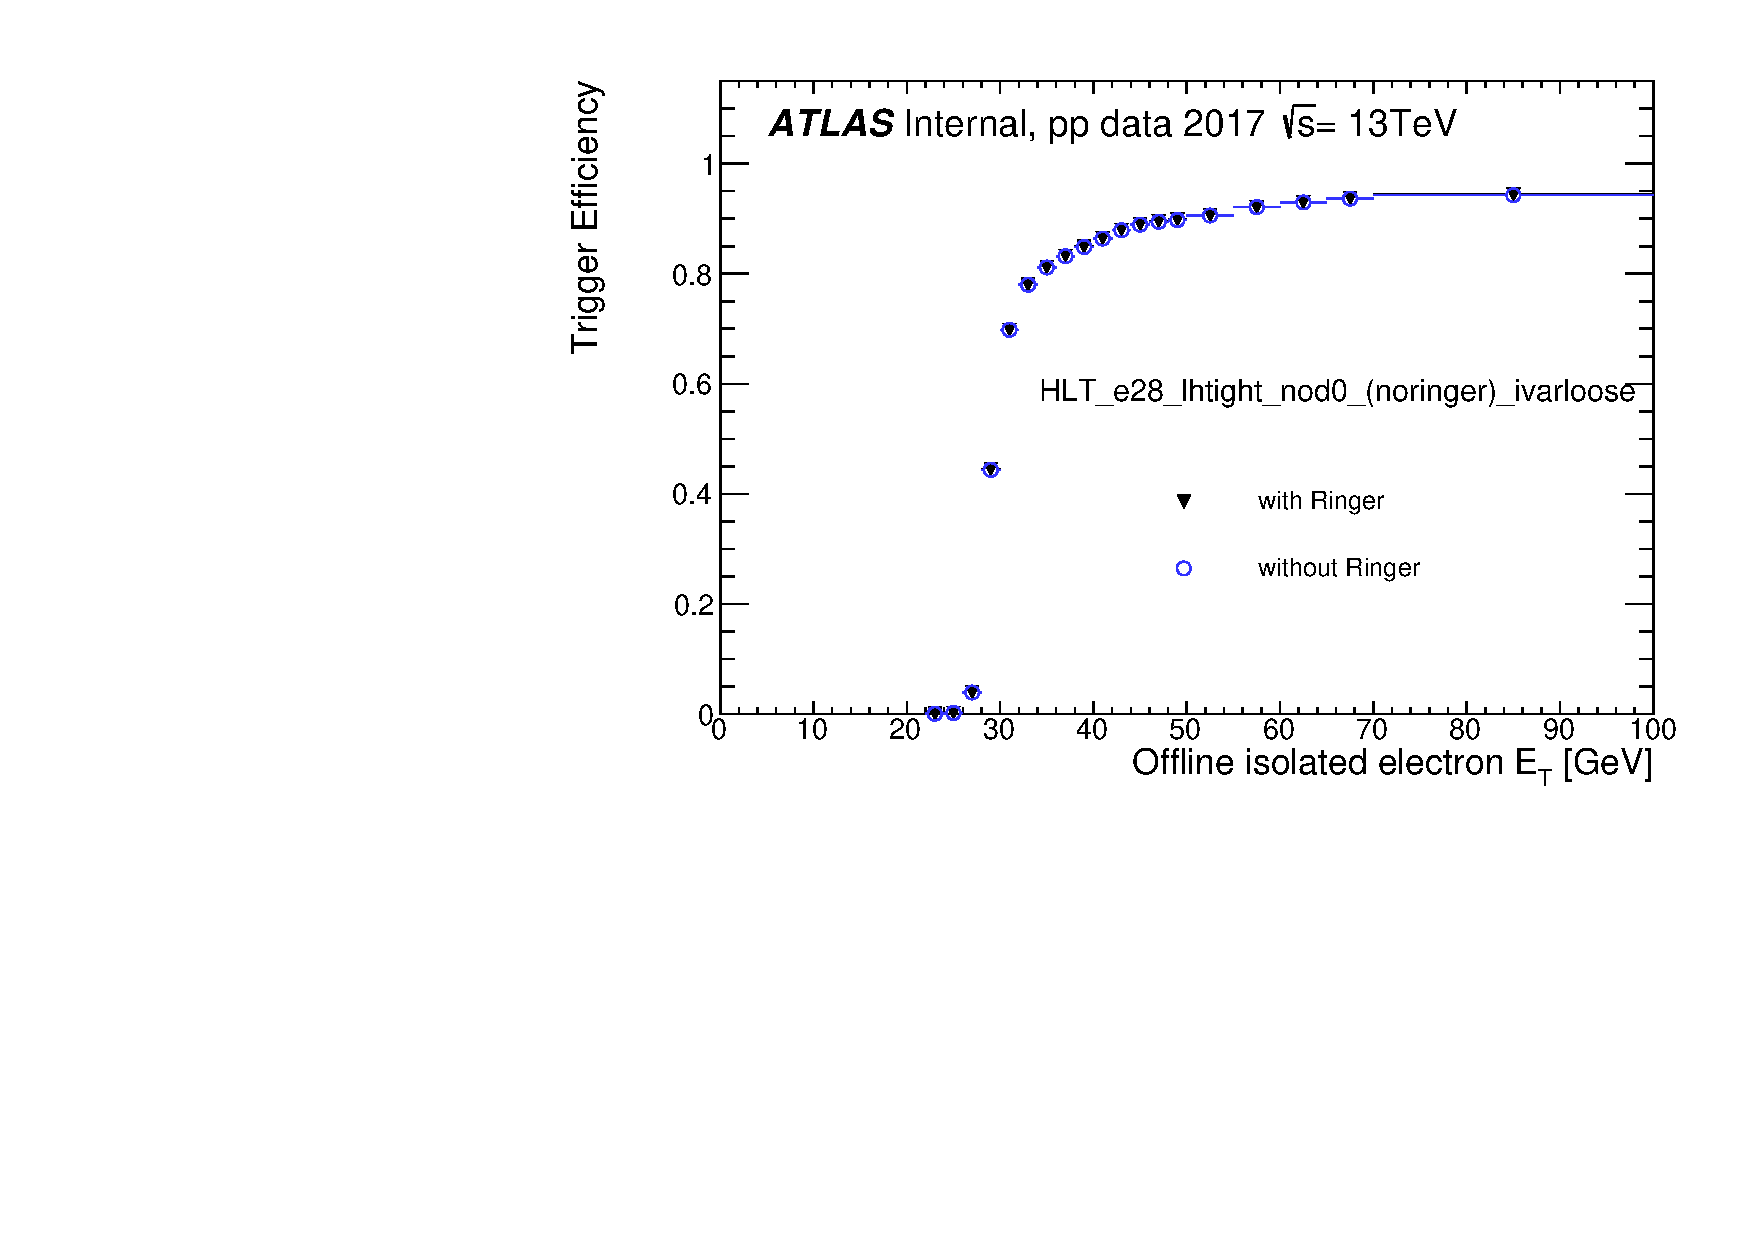
\includegraphics[width=\textwidth]{sections/04_operation/figures/efficiencies/eff_EGAM1_e28_ringer_and_noringer_2017_after_ts1_HLT_et.pdf}
  \caption{}%

  \end{subfigure} \\
  %\hfill
  %\hspace{0.01\textwidth}
  \begin{subfigure}[c]{.59\textwidth}
  \centering
  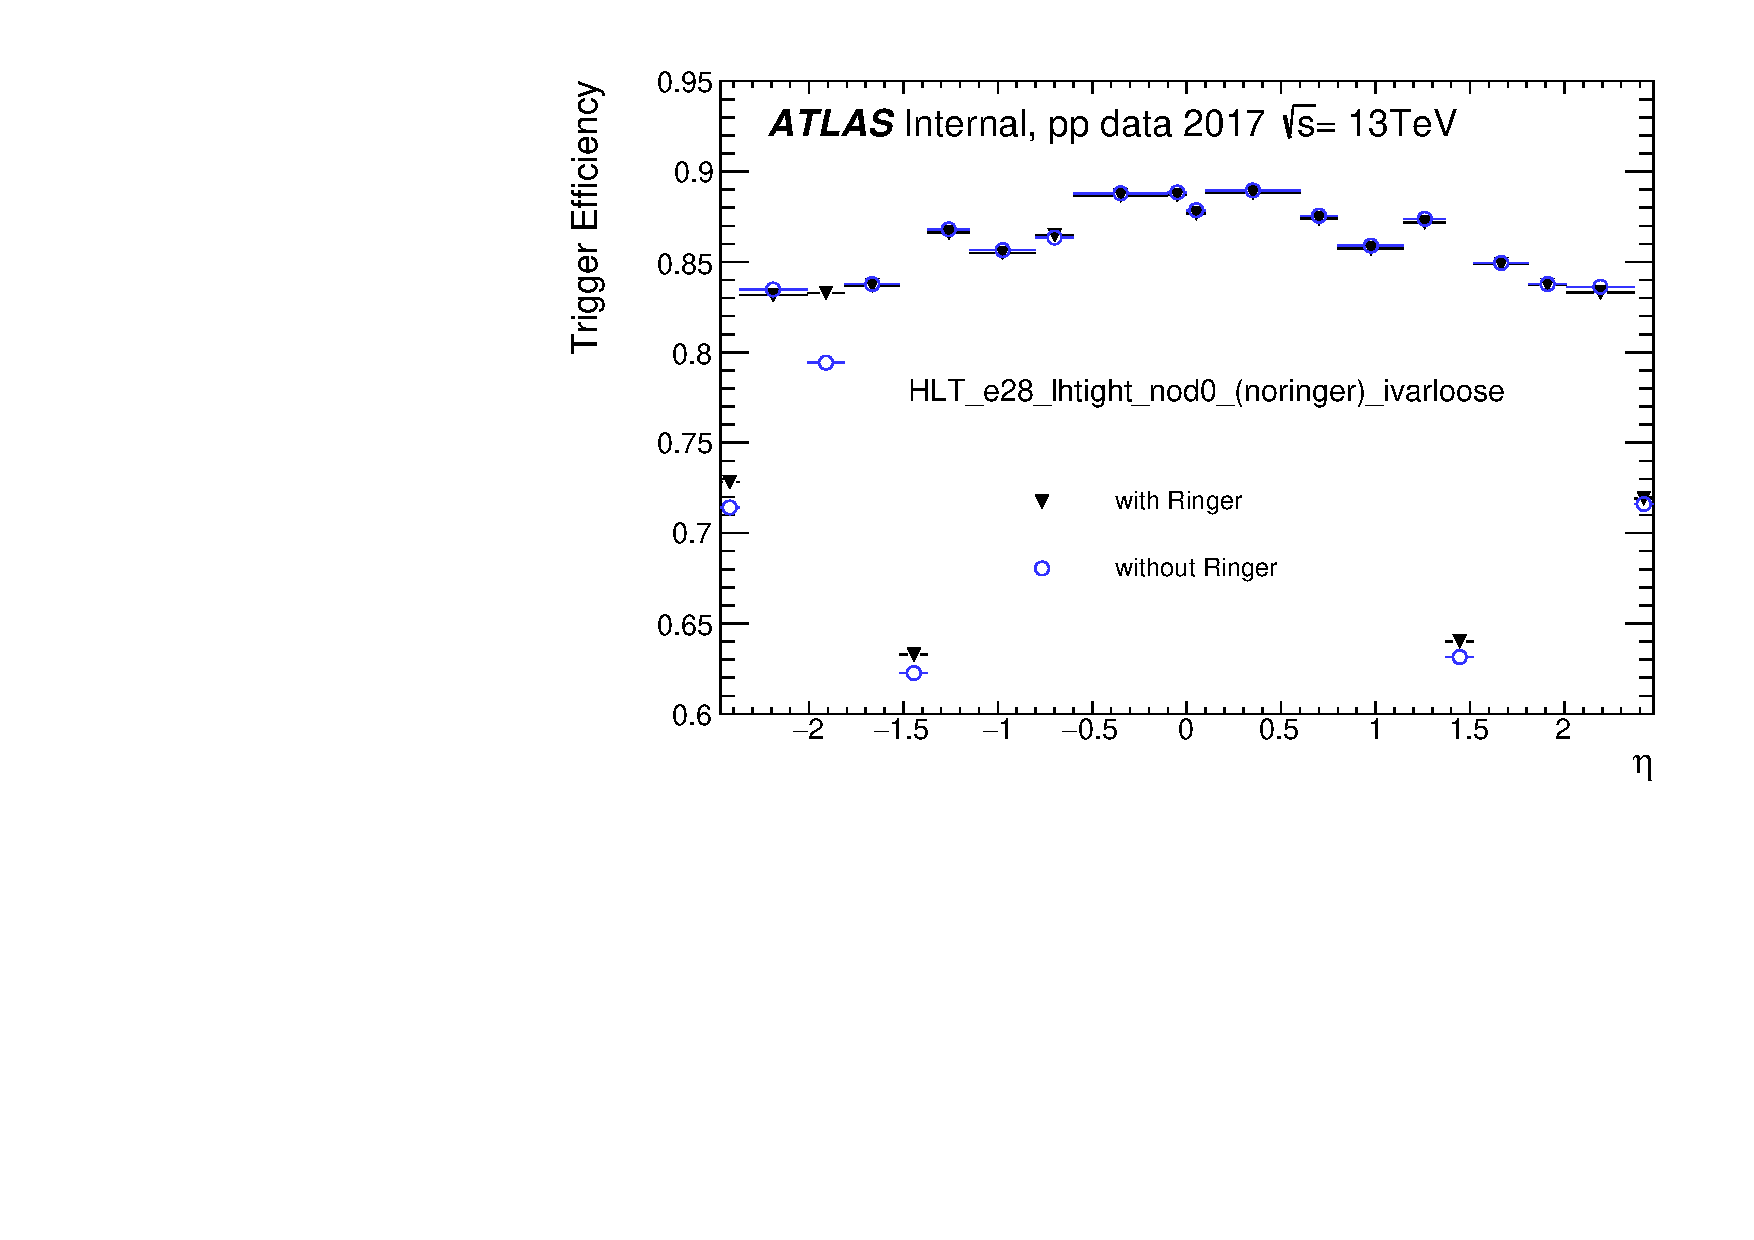
\includegraphics[width=\textwidth]{sections/04_operation/figures/efficiencies/eff_EGAM1_e28_ringer_and_noringer_2017_after_ts1_HLT_eta.pdf}
  \caption{}%
  %\label{fig:e28_comp_eta}
  \end{subfigure} \\
  \begin{subfigure}[c]{.59\textwidth}
  \centering
  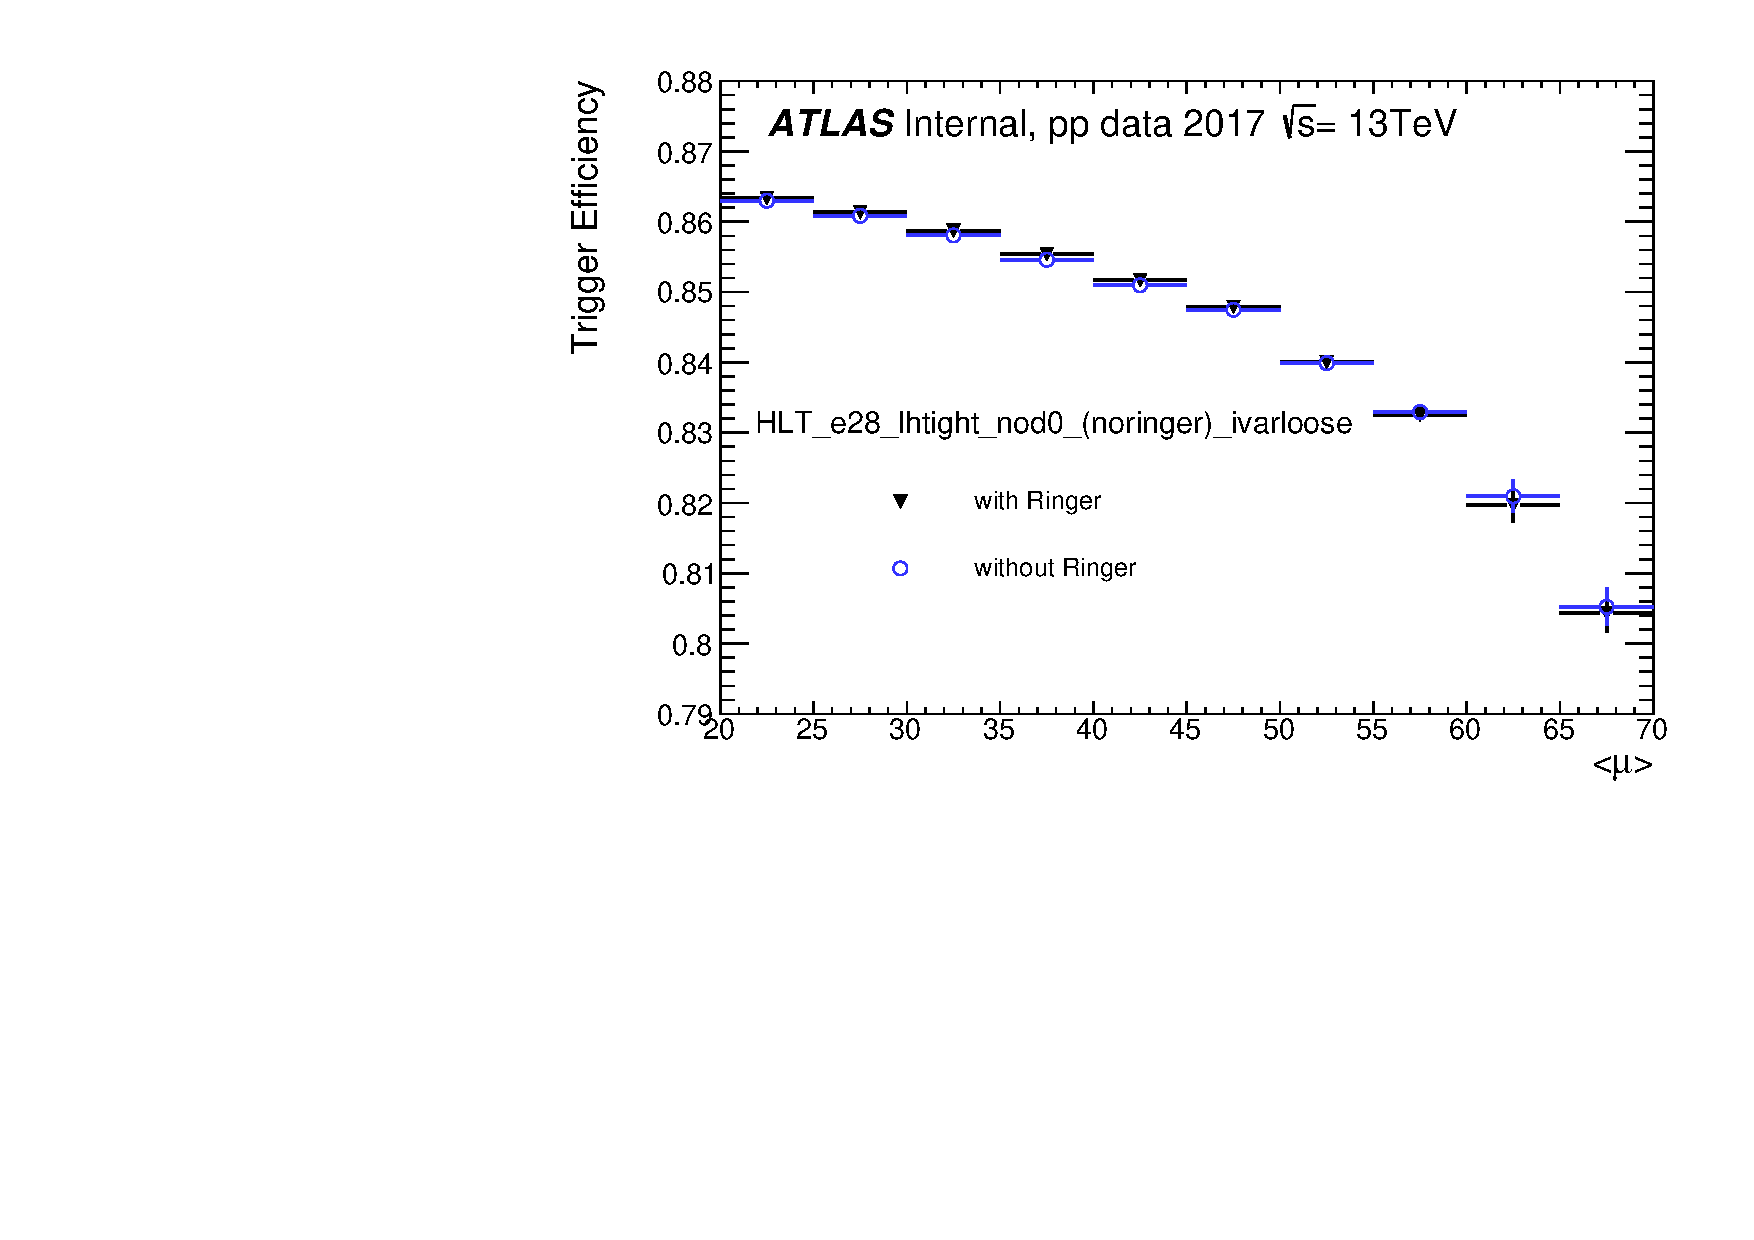
\includegraphics[width=\textwidth]{sections/04_operation/figures/efficiencies/eff_EGAM1_e28_ringer_and_noringer_2017_after_ts1_HLT_mu.pdf}
  \caption{}%
  \label{fig:e28_comp_mu}
  \end{subfigure}
  \caption{\label{fig:e28_triggers}HLT electron efficiency as a function of \et{}
    (a), \eta{} (b) and \avgmu{} (c) for the duplicated single electron isolated trigger
    requiring $\et{} > \SI{28}{\GeV}$ and \tight{} selection with and without the
    \rnn{} algorithm. Efficiencies are measured employing 2017 data collected.}
  \end{center}
\end{figure}
  
\begin{figure}[h!tb]
  \begin{center}
  \begin{subfigure}[c]{.59\textwidth}
  \centering
  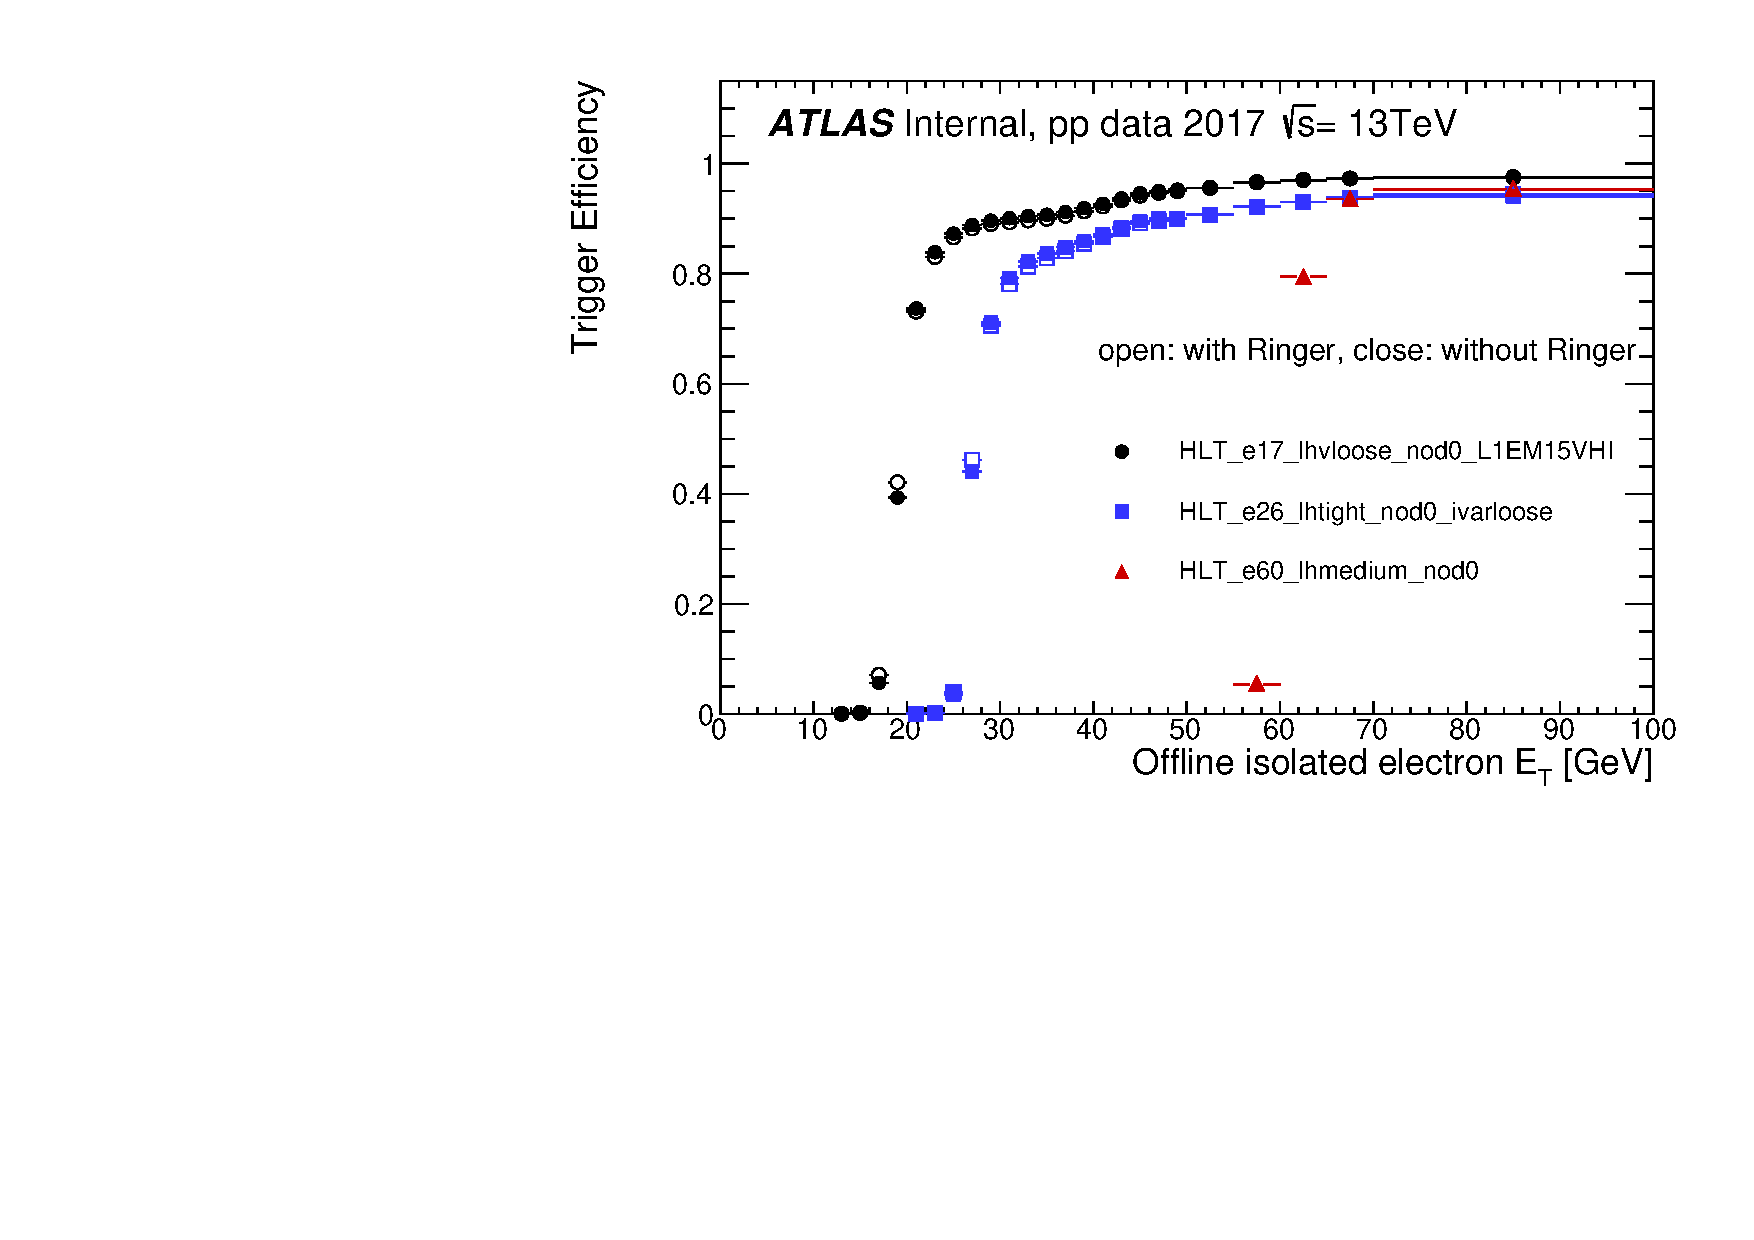
\includegraphics[width=\textwidth]{sections/04_operation/figures/efficiencies/eff_EGAM1_e17_e26_e60_2017_before_and_after_ts1_et.pdf}
  \caption{}%
  \end{subfigure}\\
  %\hfill
  %\hspace{0.01\textwidth}
  \begin{subfigure}[c]{.59\textwidth}
  \centering
  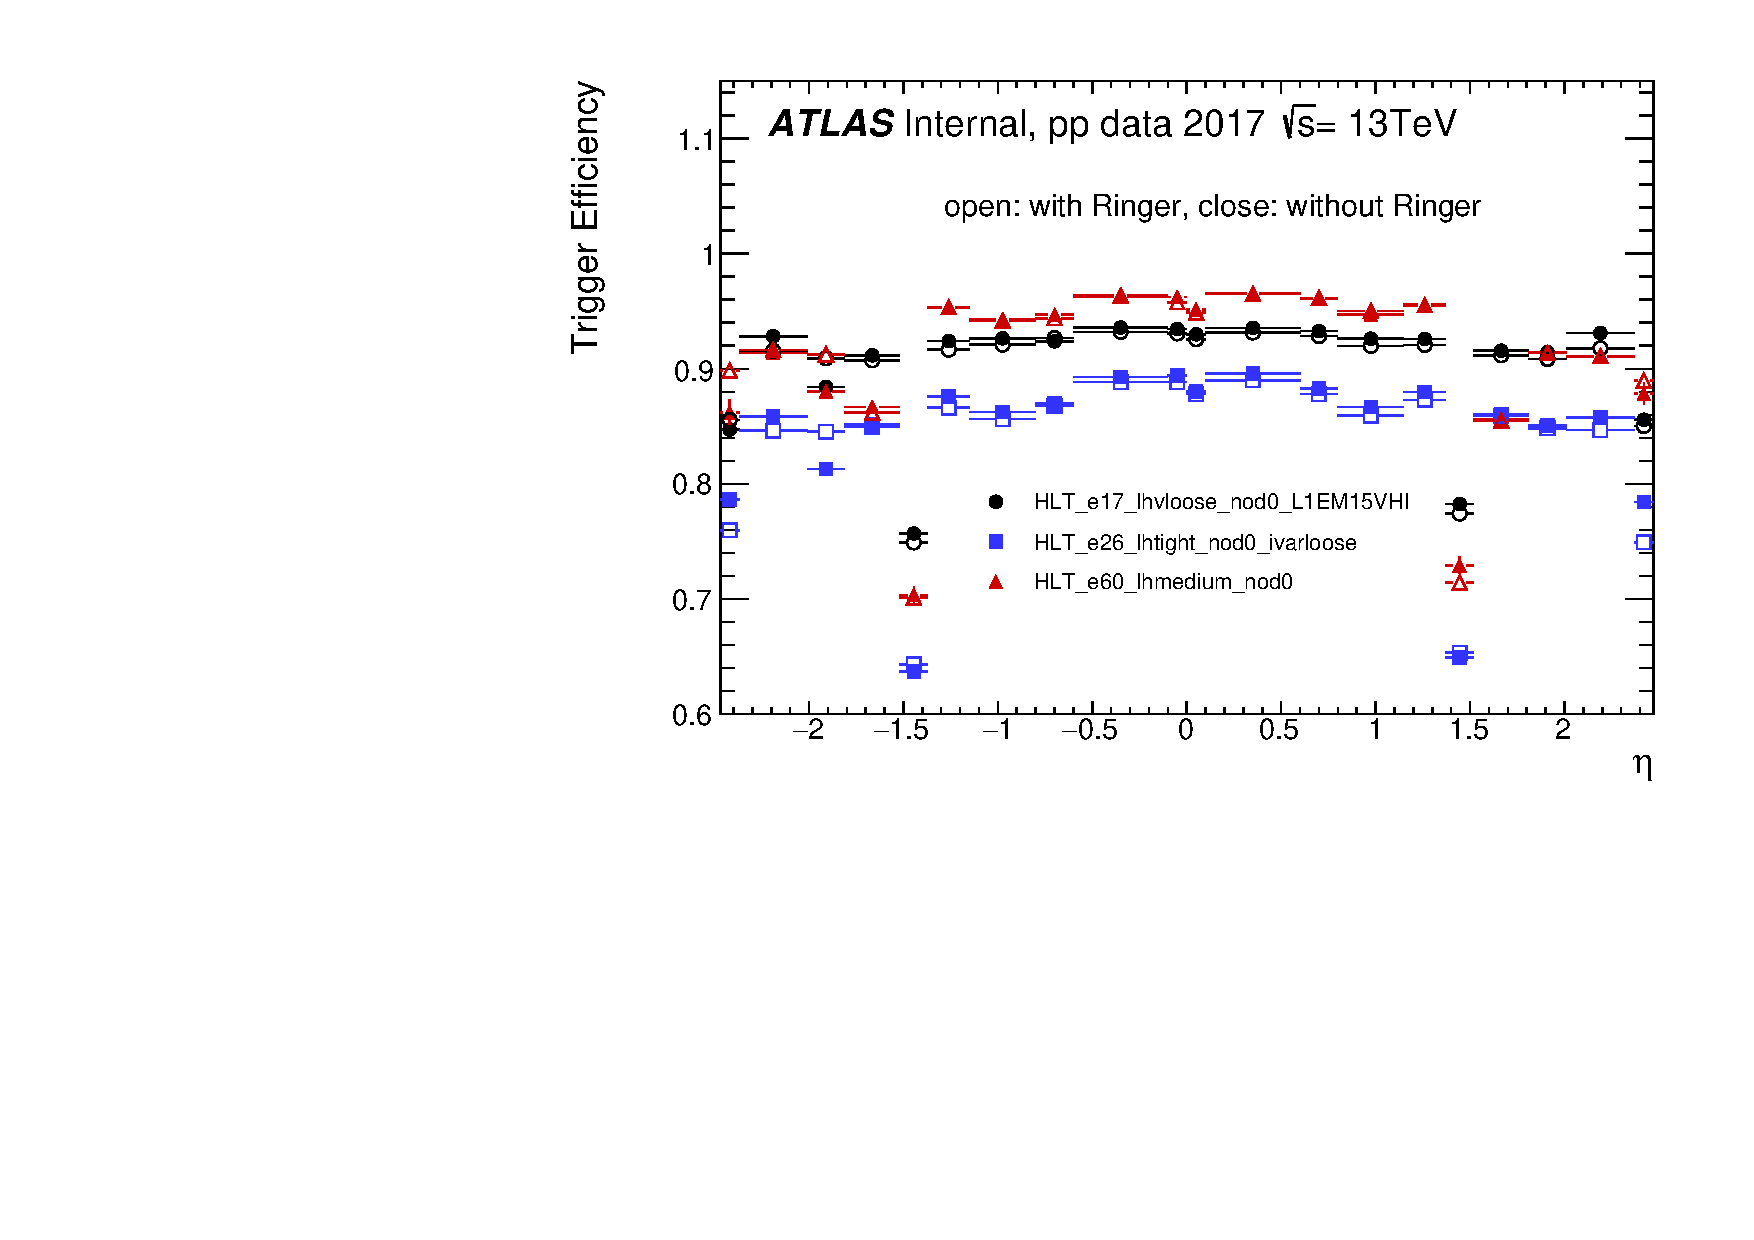
\includegraphics[width=\textwidth]{sections/04_operation/figures/efficiencies/eff_EGAM1_e17_e26_e60_2017_before_and_after_ts1_eta.pdf}
  \caption{}%
  \end{subfigure} \\
  \begin{subfigure}[c]{.59\textwidth}
  \centering
  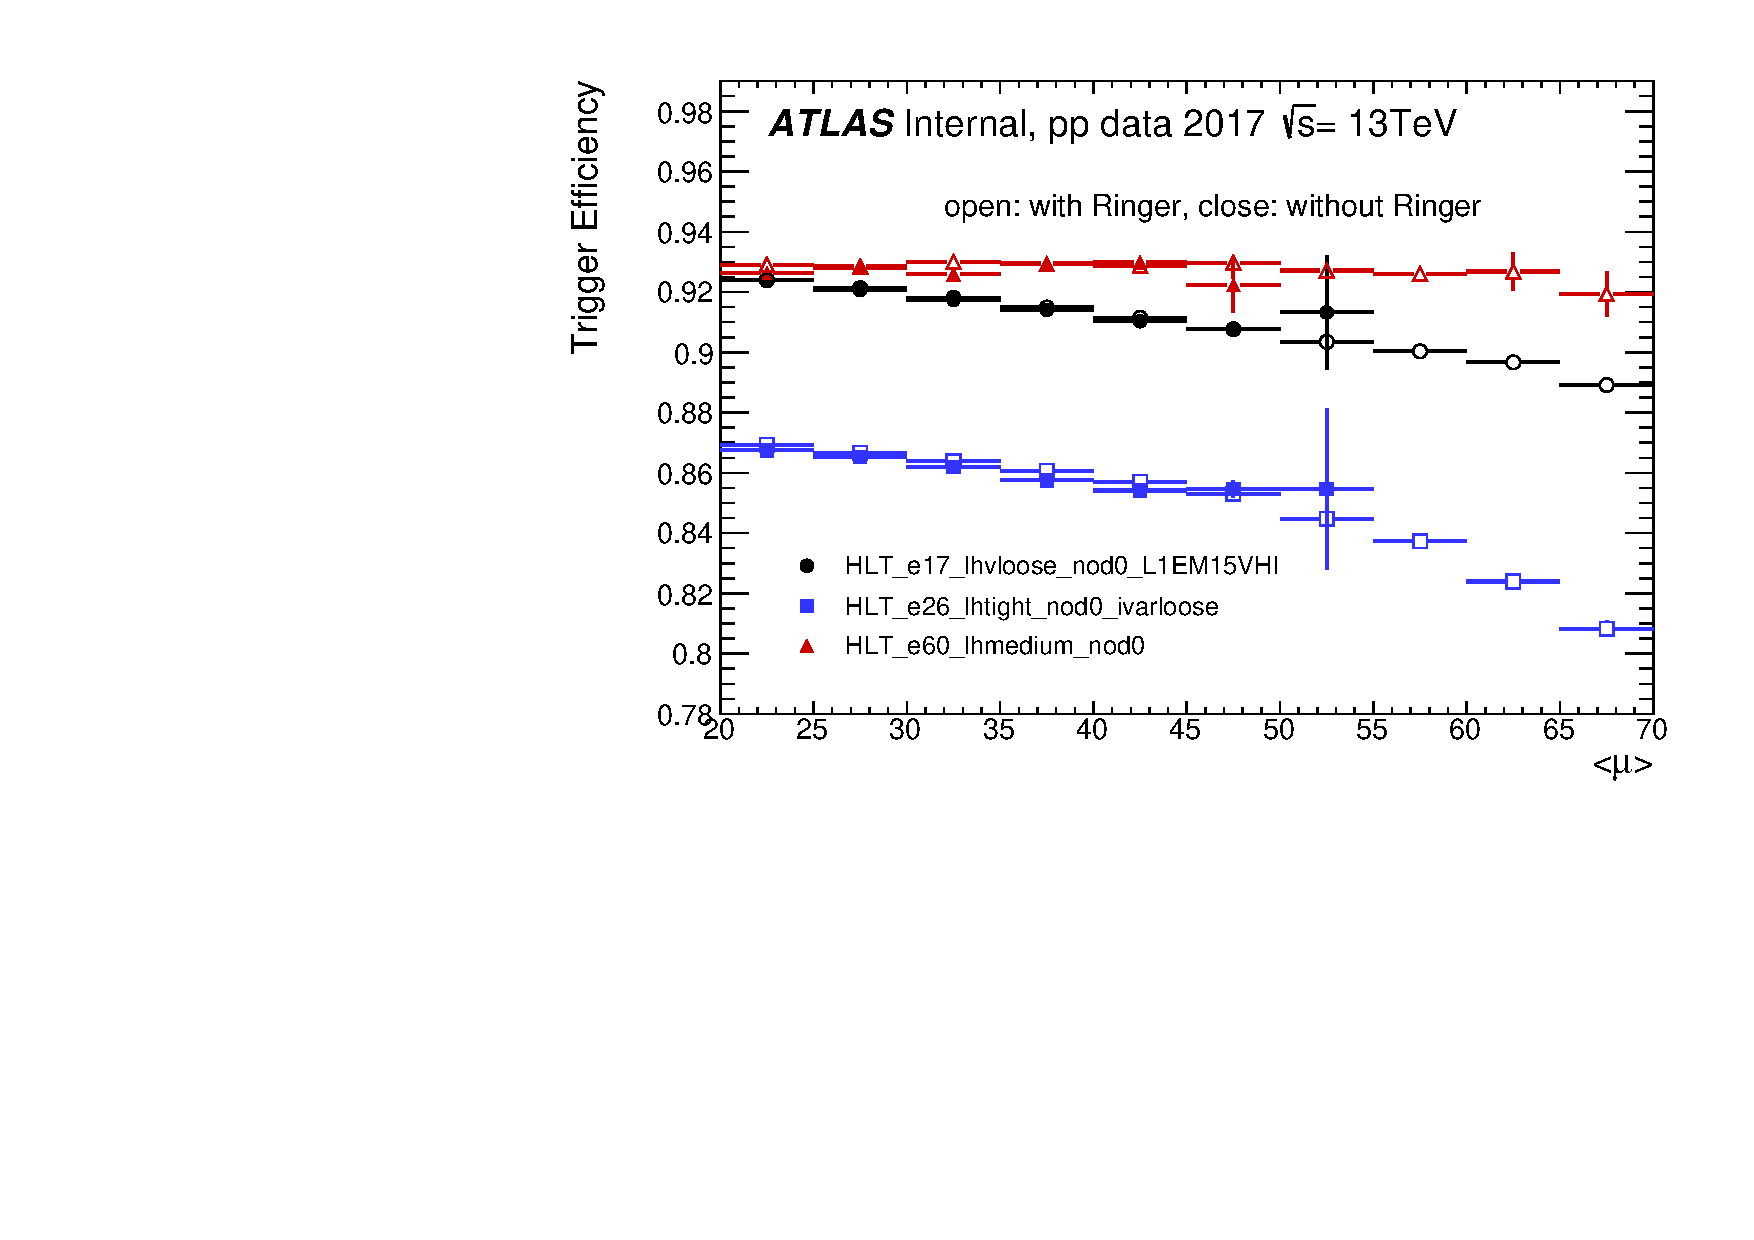
\includegraphics[width=\textwidth]{sections/04_operation/figures/efficiencies/eff_EGAM1_e17_e26_e60_2017_before_and_after_ts1_mu.pdf}
  \caption{}%
  \end{subfigure}
  %\hfill
  \caption{Efficiency of three single electron triggers as a function of
  \et (a), \eta (b) and \avgmu (c). Open (closed) markers contain
  the efficiency measurements on runs before (after) the first technical stop, thus referring to
  triggers being executed without (with) the \rnn{} algorithm. For 2017 collision data, the higher \avgmu{} values were reached only after the technical stop. 
  }%
  \label{fig:2017_ts1}
  \end{center}
\end{figure}


By contrasting the behavior of the duplicated trigger using fake electron data,
it becomes clear the power of the \rnn{} algorithm. An overall reduction factor of
the fake rate by a factor of 13.75 is achieved. It can be seen in
Figure~\ref{fig:e28_triggers_fake} that the improvement is similar for all
regions in the evaluated variables, particularly interesting when
considering the low \et{} and the end-cap regions.




\begin{figure}[h!tb]
  \begin{center}
  \begin{subfigure}[c]{.59\textwidth}
  \centering
  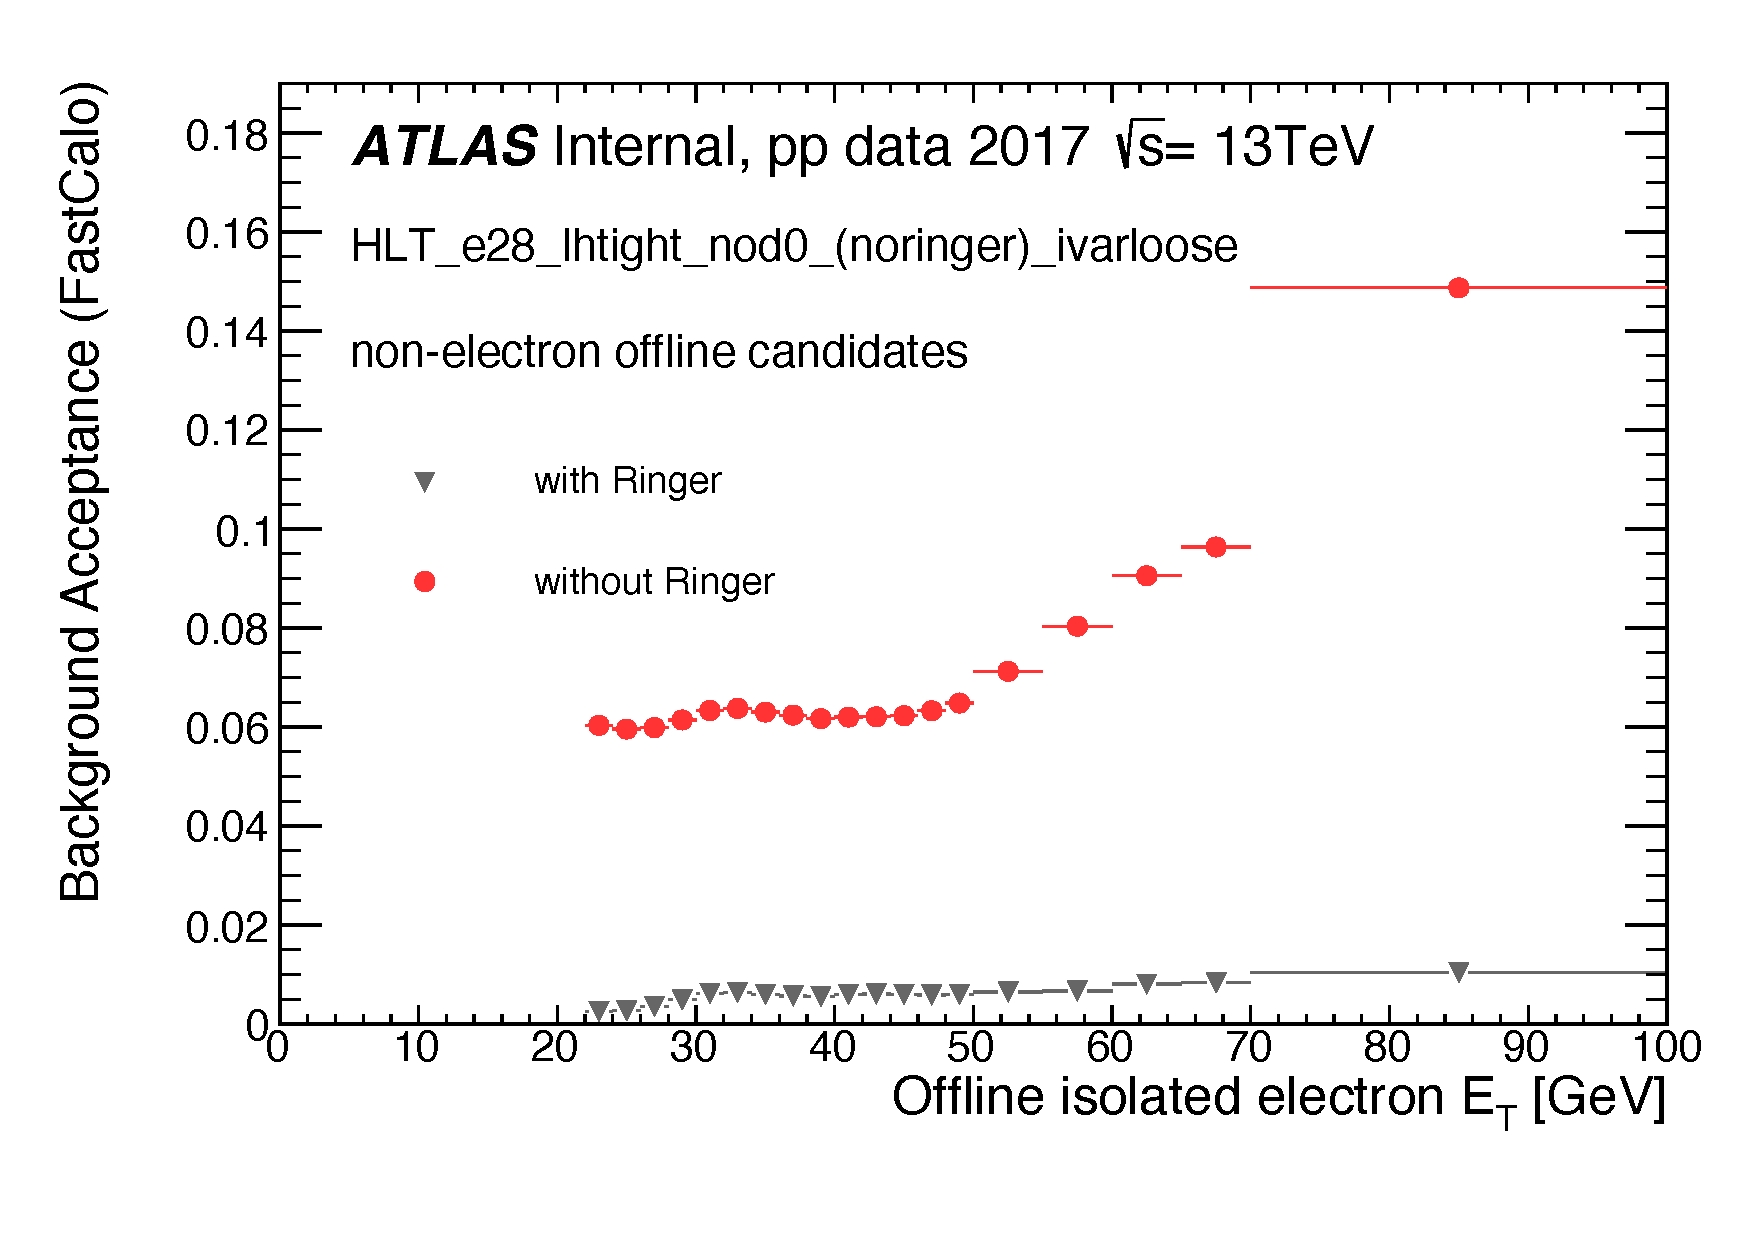
\includegraphics[width=\textwidth]{sections/04_operation/figures/efficiencies/eff_EGAM7_e28_ringer_and_noringer_2017_after_ts1_L2Calo_et.pdf}
  %\label{fig:e28_comp_et_fake}
  \caption{}
  \end{subfigure}\\
  %\hfill
  %\hspace{0.01\textwidth}
  \begin{subfigure}[c]{.59\textwidth}
  \centering
  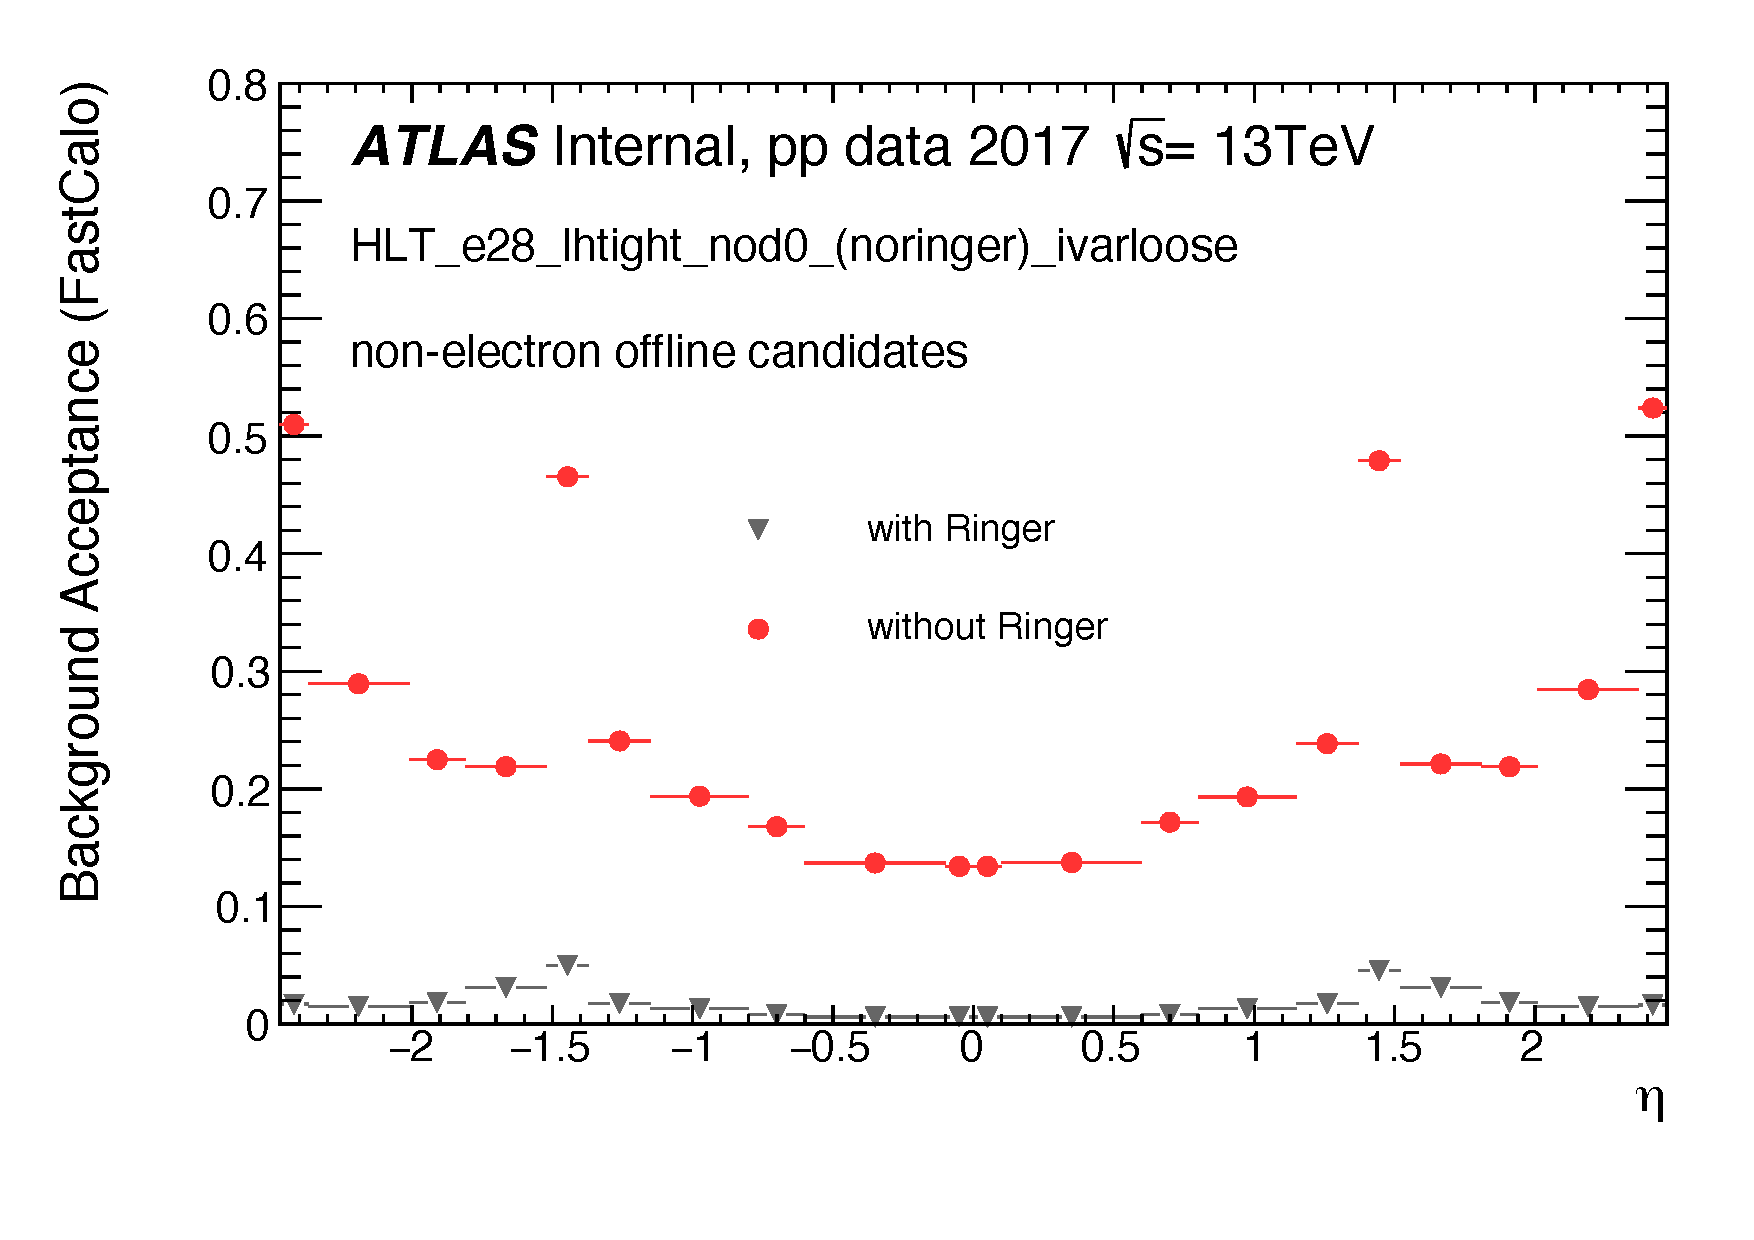
\includegraphics[width=\textwidth]{sections/04_operation/figures/efficiencies/eff_EGAM7_e28_ringer_and_noringer_2017_after_ts1_L2Calo_eta.pdf}
  %\label{fig:e28_comp_eta_fake}
  \caption{}
  \end{subfigure}\\
  \begin{subfigure}[c]{.59\textwidth}
  \centering
  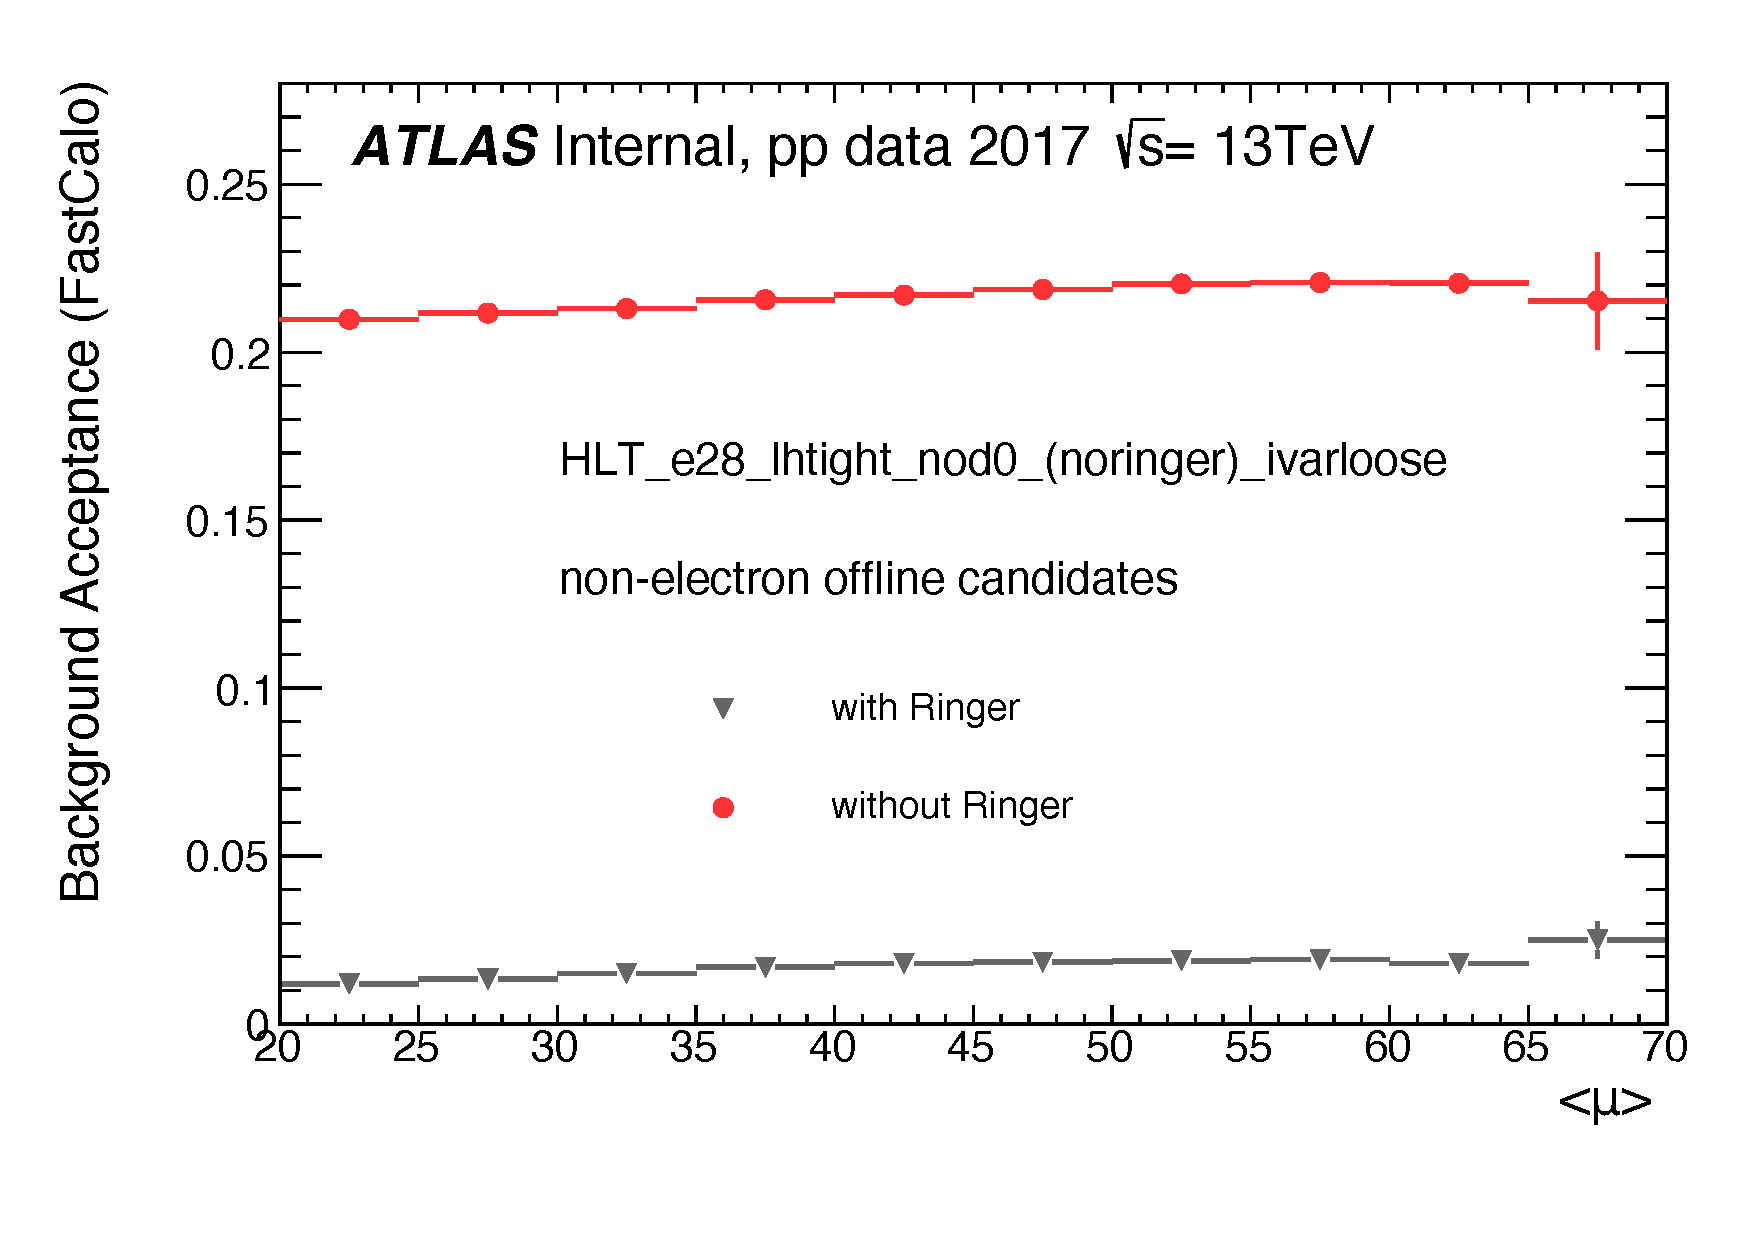
\includegraphics[width=\textwidth]{sections/04_operation/figures/efficiencies/eff_EGAM7_e28_ringer_and_noringer_2017_after_ts1_L2Calo_mu.pdf}
  %\label{fig:e28_comp_mu_fake}
  \caption{}
  \end{subfigure}
  %\hfill
  \caption{\label{fig:e28_triggers_fake} \fastcalo %\footnotemark{} 
  fake electron efficiency as a function of \et (a), \eta (b) and \avgmu (c) for the
  duplicated single electron isolated trigger requiring $\et > \SI{28}{\GeV}$ and \tight
  selection with and without the \rnn{} algorithm. Efficiencies are measured
  employing 2017 data collected after the first technical stop.}%
  
  \end{center}
\end{figure}



Besides the capability of improving early fake rejection, the usage of the
\rnn{} also contributed to reduce the final fake rate
(Figure~\ref{fig:e28_triggers_fake_hlt}) by a factor of 2, mostly coming from
the transition regions in the calorimeter. The discussion about CPU and final rate reduction will be covered in the next section.

 %This fake rate reduction when measured with
%respect to the offline electron selection does not seem to have impacted in the
%output rate (see Appendix~\ref{ssec:primary_rate_wrt_luminosity})\footnote{This
%  can provide some indication that measuring background efficiencies with
%respect to the offline may not be the best approach.}, but may have
%contributed to reduce signal contamination in physics analyses.

\begin{figure}[h!tb]
\begin{center}
\begin{subfigure}[c]{.59\textwidth}
\centering
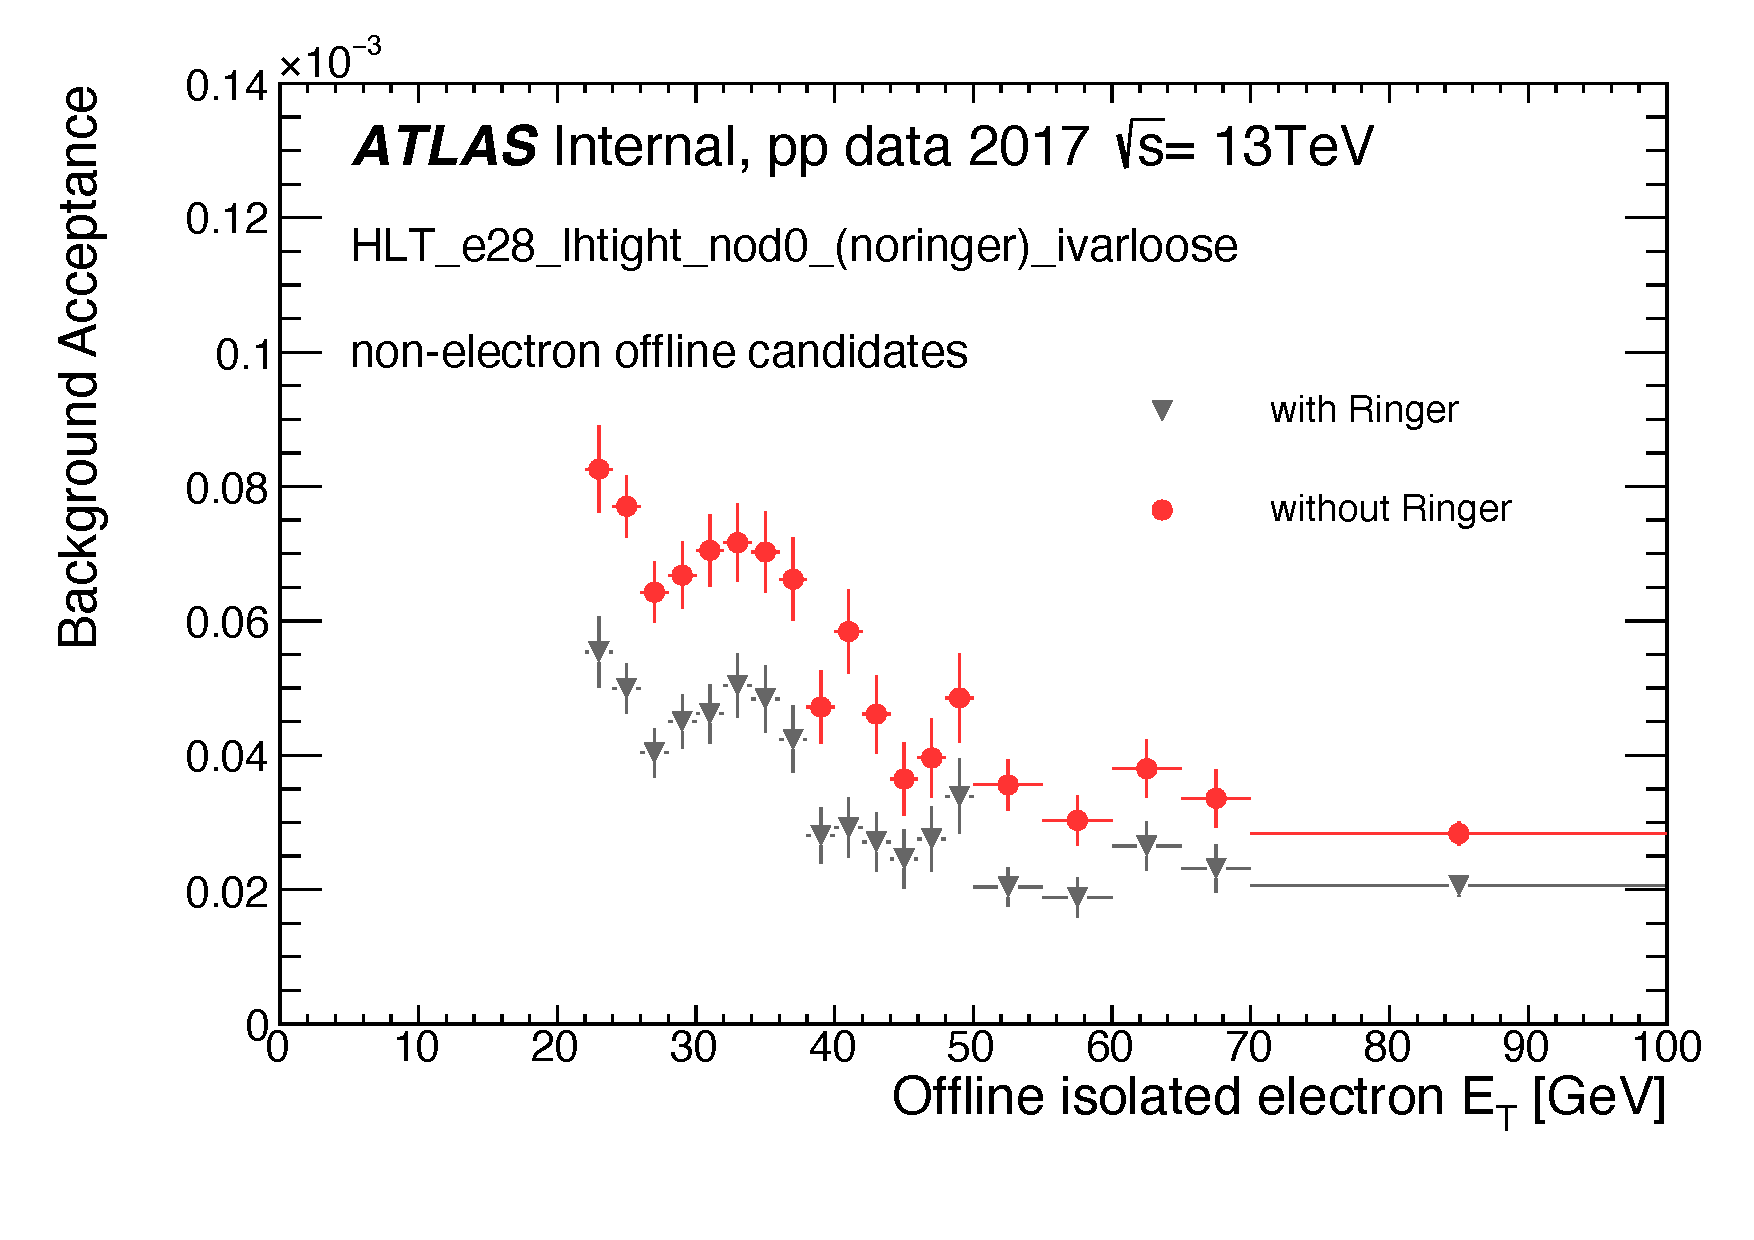
\includegraphics[width=\textwidth]{sections/04_operation/figures/efficiencies/eff_EGAM7_e28_ringer_and_noringer_2017_after_ts1_et.pdf}
\caption{}
\end{subfigure}\\
%\hfill
%\hspace{0.01\textwidth}
\begin{subfigure}[c]{.59\textwidth}
\centering
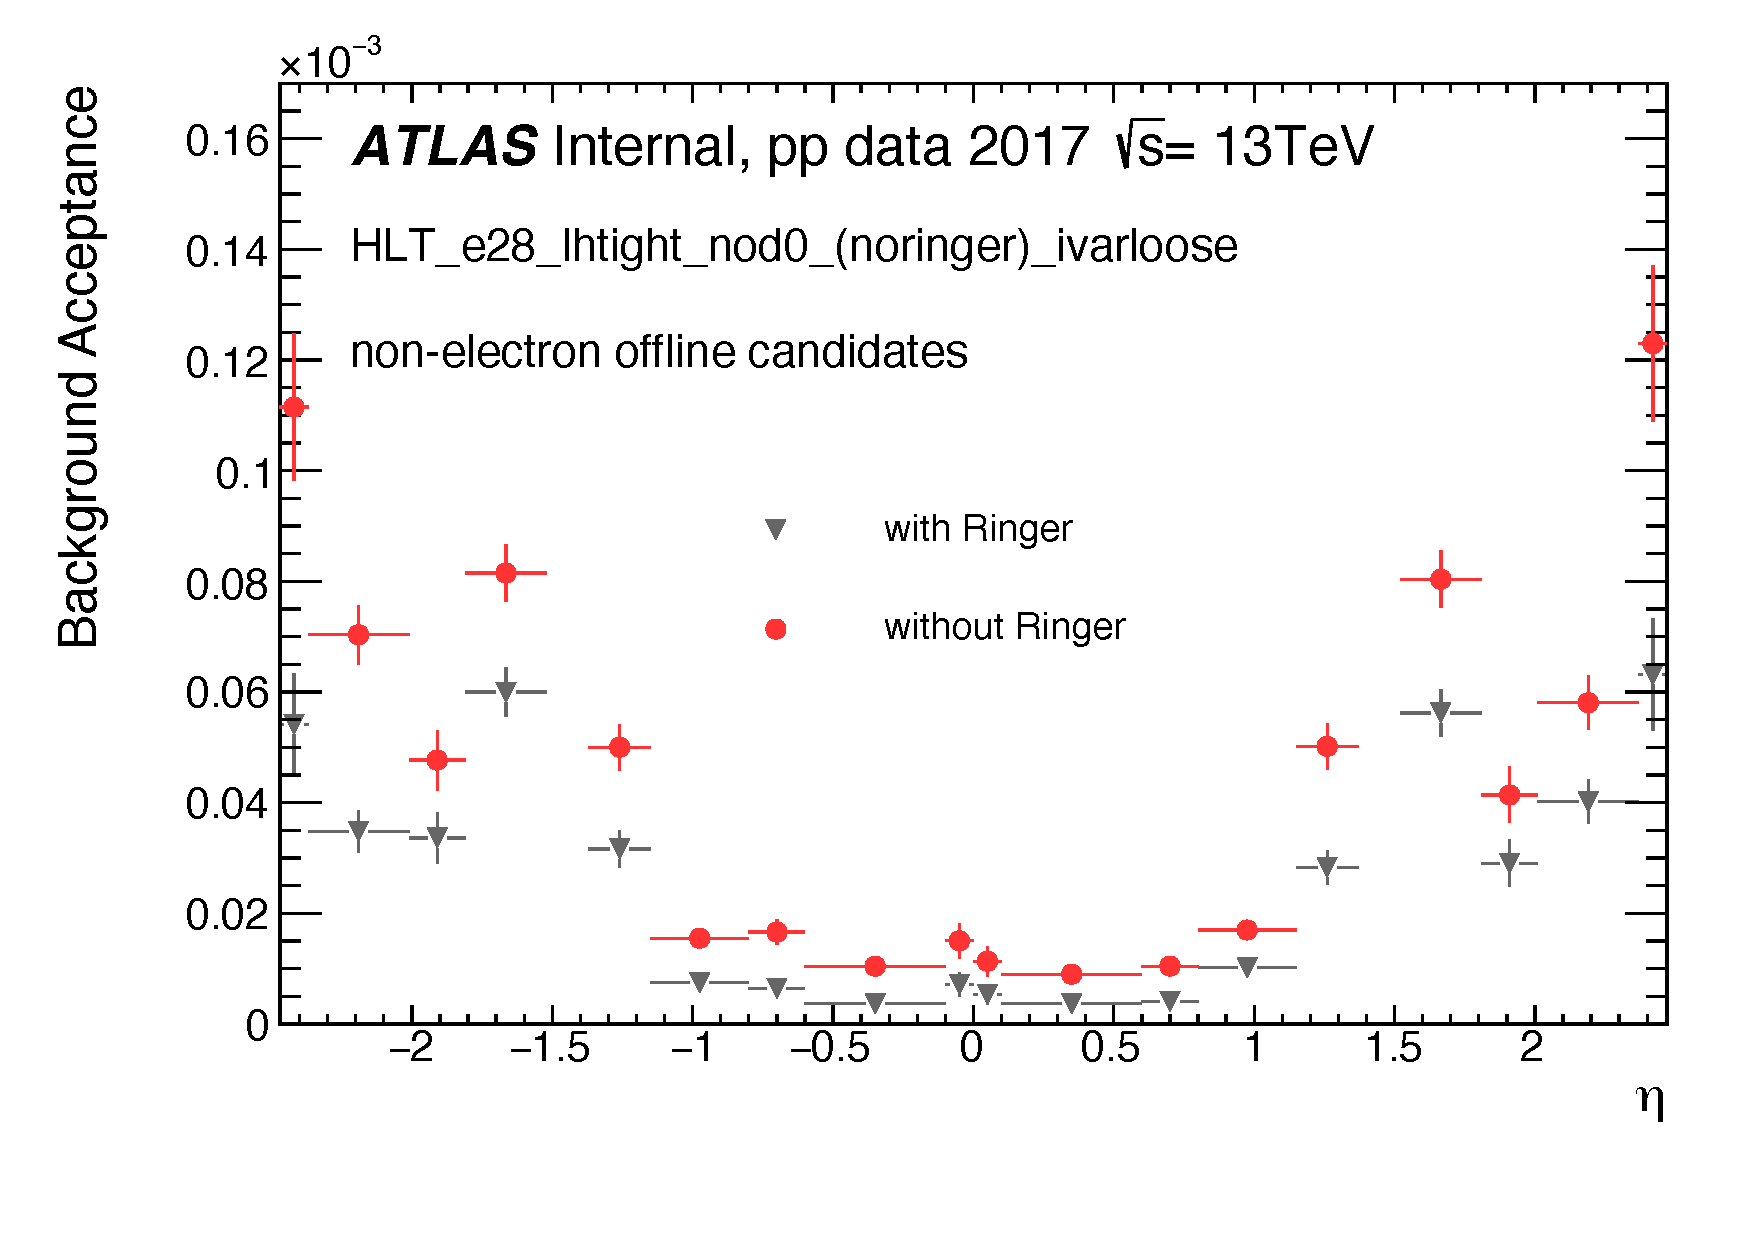
\includegraphics[width=\textwidth]{sections/04_operation/figures/efficiencies/eff_EGAM7_e28_ringer_and_noringer_2017_after_ts1_eta.pdf}
\caption{}
\end{subfigure} \\
\begin{subfigure}[c]{.59\textwidth}
\centering
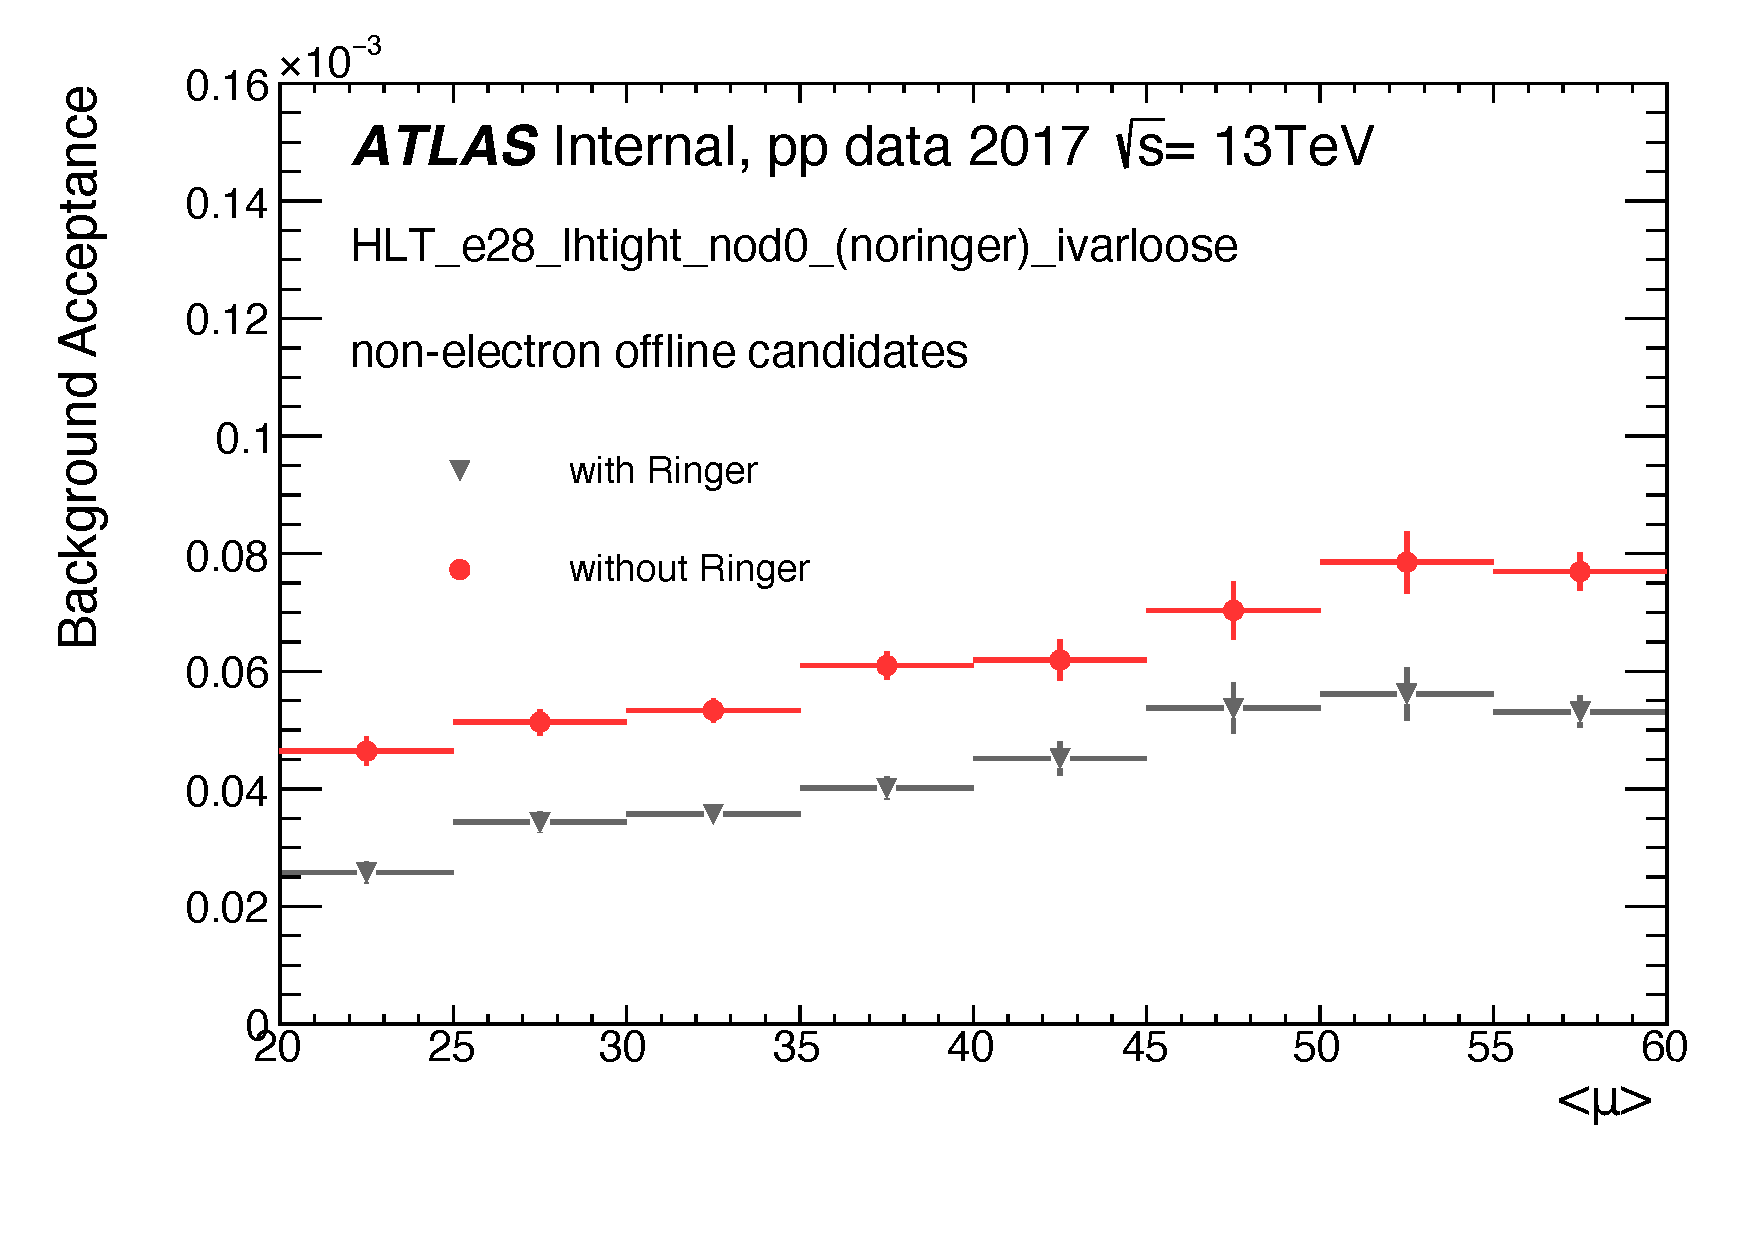
\includegraphics[width=\textwidth]{sections/04_operation/figures/efficiencies/eff_EGAM7_e28_ringer_and_noringer_2017_after_ts1_mu.pdf}
\caption{}
\end{subfigure}
\caption{HLT fake electron efficiency as a function of \et (a), \eta (b) and
\avgmu (c) for the duplicated single electron isolated trigger requiring $\et >
\SI{28}{\GeV}$ and \tight selection with and without the \rnn{} algorithm.
Efficiencies are measured employing 2017 data collected after the first technical stop.}%
\label{fig:e28_triggers_fake_hlt}
\end{center}
\end{figure}


\FloatBarrier

\section{2018 Operation}\label{ssec:2018_ringer_operation}

In 2018, the \rnn{} operated with a new tune based on collision data
(Section~\ref{ssec:2018}). It was also the case for the final HLT
selection\footnote{One exception was the \medium{} selection, where the HLT
likelihood selection operated in 2018 with the same 2017 tune.}. For the
lowest-transverse energy-threshold unprescaled trigger, an efficiency
improvement of at least one percentage point in central value is observed when
comparing both periods, resulting from a better operation in all selection
steps, but, in particular, this is due to improvements from the likelihood tunes in the period.

Despite maintaining high electron efficiency, it was observed a small reduction in fake acceptance at \fastcalo{} for some unprescaled triggers in comparison with 2017 after TS1. For the lowest-transverse energy-threshold it is observed a reduction factor by 1.19. On the other hand, for the highest-transverse energy trigger, a reduction factor by 1.69 was achieved.


 % ok

\chapter{\rnn{} Performance}%
\label{sec:off_ana}

This section dedicates to more detailed assessments of the \rnn{} behavior 
in the period 2017-2018 with respect to the previous electron trigger cut-based strategy.
Using \Zee{} \tnp{}
selection, we investigate the agreement between the two triggers and investigate
for possible biases caused by the introduction of the \rnn{} using the variables
employed by the likelihood algorithm. Since offline and final HLT electron
selection are based on such variables, limiting the evaluation to them suffice
to understand any possible impact of the \rnn{} algorithm in most analyses.
Additionally, these variables are interesting since they compact the input space
in a set of few variables with low correlation and high interpretability power. One should keep in mind that the \rnn{} algorithm had access only to the ring description during Run~2 operation.

As indicated in Table~\ref{tab:quadrant_vs_agreement}, we perform two analyses evaluating the
trigger performance with and without \rnn{}, when applied to the tag (Agreement Analysis) and
to the probe (Quadrant Analysis). The Tag \& Probe events have one probe electron that was not used to decide the selection of that event at the trigger level.


\begin{table}[ht!]\footnotesize
\centering
\caption{Customized \Zee{} \tap{} selection criteria employed in the
agreement and quadrant analyses in the Run 2 (2017-2018 period)}.%
\label{tab:quadrant_vs_agreement}
\resizebox{\textwidth}{!}{%
  \begin{tabular}{p{2cm}p{4.5cm}p{5.5cm}}
\hline
\hline
\hline
& Agreement Analysis (Section~\ref{ssec:agreement}) & Quadrant Analysis
(Section~\ref{ssec:quadrant}) \\
\hline
\hline
tag (and event) & trigger selection comparison & primary lowest unprescaled electron triggers \\
\hline
probe & \vloose & trigger selection comparison with offline selection fixed to
the same trigger requirement \\
\hline
\hline
\hline
\end{tabular}
}
\end{table}

The Quadrant Analysis allows to directly assess possible bias caused by the
introduction of the \rnn{} by comparing the profiles for all possible disjoint
decisions from the two trigger classifiers. Hence, it is possible for the classifiers
to agree by both accepting or rejecting the event. Likewise, they are able to
disagree in two possible cases where either one decides to accept the event
while the other rejects it.

Although it is reasonable to expect that the shower development of the tag and
the probe are independent from each other, and that the \rnn{} when applied to
the tag selection cannot, in principle, alter the profile of the probes besides
changing the number of \tnp{} pairs, such evaluation of systematic effect as
performed by the Agreement Analysis is interesting for allowing to evaluate any
possible systematic effect caused by the introduction of the \rnn{} in the extraction of the likelihood PDFs employed for offline and final HLT selection.

\FloatBarrier
\section{Impact on CPU Demands} %\label{ssec:cpu_reduction}

As observed in the efficiency measurements during Run~2 data taking, the \rnn{}
allowed more effective \fastcalo{} operation in triggers with electron legs
above \SI{15}{\GeV}  with respect to the previous cut-based approach. In this section, we evaluate how the more efficient trigger
configuration improves the online system in terms of resource requirements.
First, we investigate the CPU requirements at the \fastcalo{}
level (Section~\ref{top:fastcalo_cpu}). We then address the full impact of CPU
requirements of the \rnn{} in a primary electron trigger
(Section~\ref{top:cpu_e26}).

\subsection{\fastcalo{} CPU Demands}\label{top:fastcalo_cpu}


We have evaluated the overhead required to compute the \rnn{} decision by running a single electron trigger with and without the \rnn algorithm in two individual non-concurrent executions using the same dedicated node\footnote{It was used a techlab node Xeon Phi 7120 (1.7 GHz, 32 threads) with 256 Gb@1333 of memory and a SL6 OS.}. It should be mentioned that, in order to reduce implementation efforts, electron triggers executing the \rnn{} information compute their information after the cut-based reconstruction, whose decision is not computed. As a result of this, the \rnn{} electron 
triggers always demand additional \fastcalo processing time.

Figures~\ref{fig:fastcalo_fex_time} and~\ref{fig:fastcalo_hypo_time} show the comparison of the total CPU time per event for the feature extraction and hypothesis algorithms in the \fastcalo respectively.
The CPU time does not include the online data preparation time and measurements were evaluated from a very loose selection electron trigger with individual executions in the same dedicated computer node.


The measurement employed events from enhanced bias (EB)
stream~\cite{eb_description} typically extracted from one hour acquisition with
a specific trigger menu based only on first level selection and aiming at
collecting about one million background events more likely to be accepted by the
\hlt{}. This behavior is obtained by applying an overweight in high-\pt{} region,
and at a rate of \SI{300}{\hertz}~\cite{eb_specifications}. Hence, the
measurements are performed under pile-up conditions with the execution of the
reconstructed observable algorithm for multiple RoIs in the same bunch-crossing event.


\begin{figure}[h!tb]
	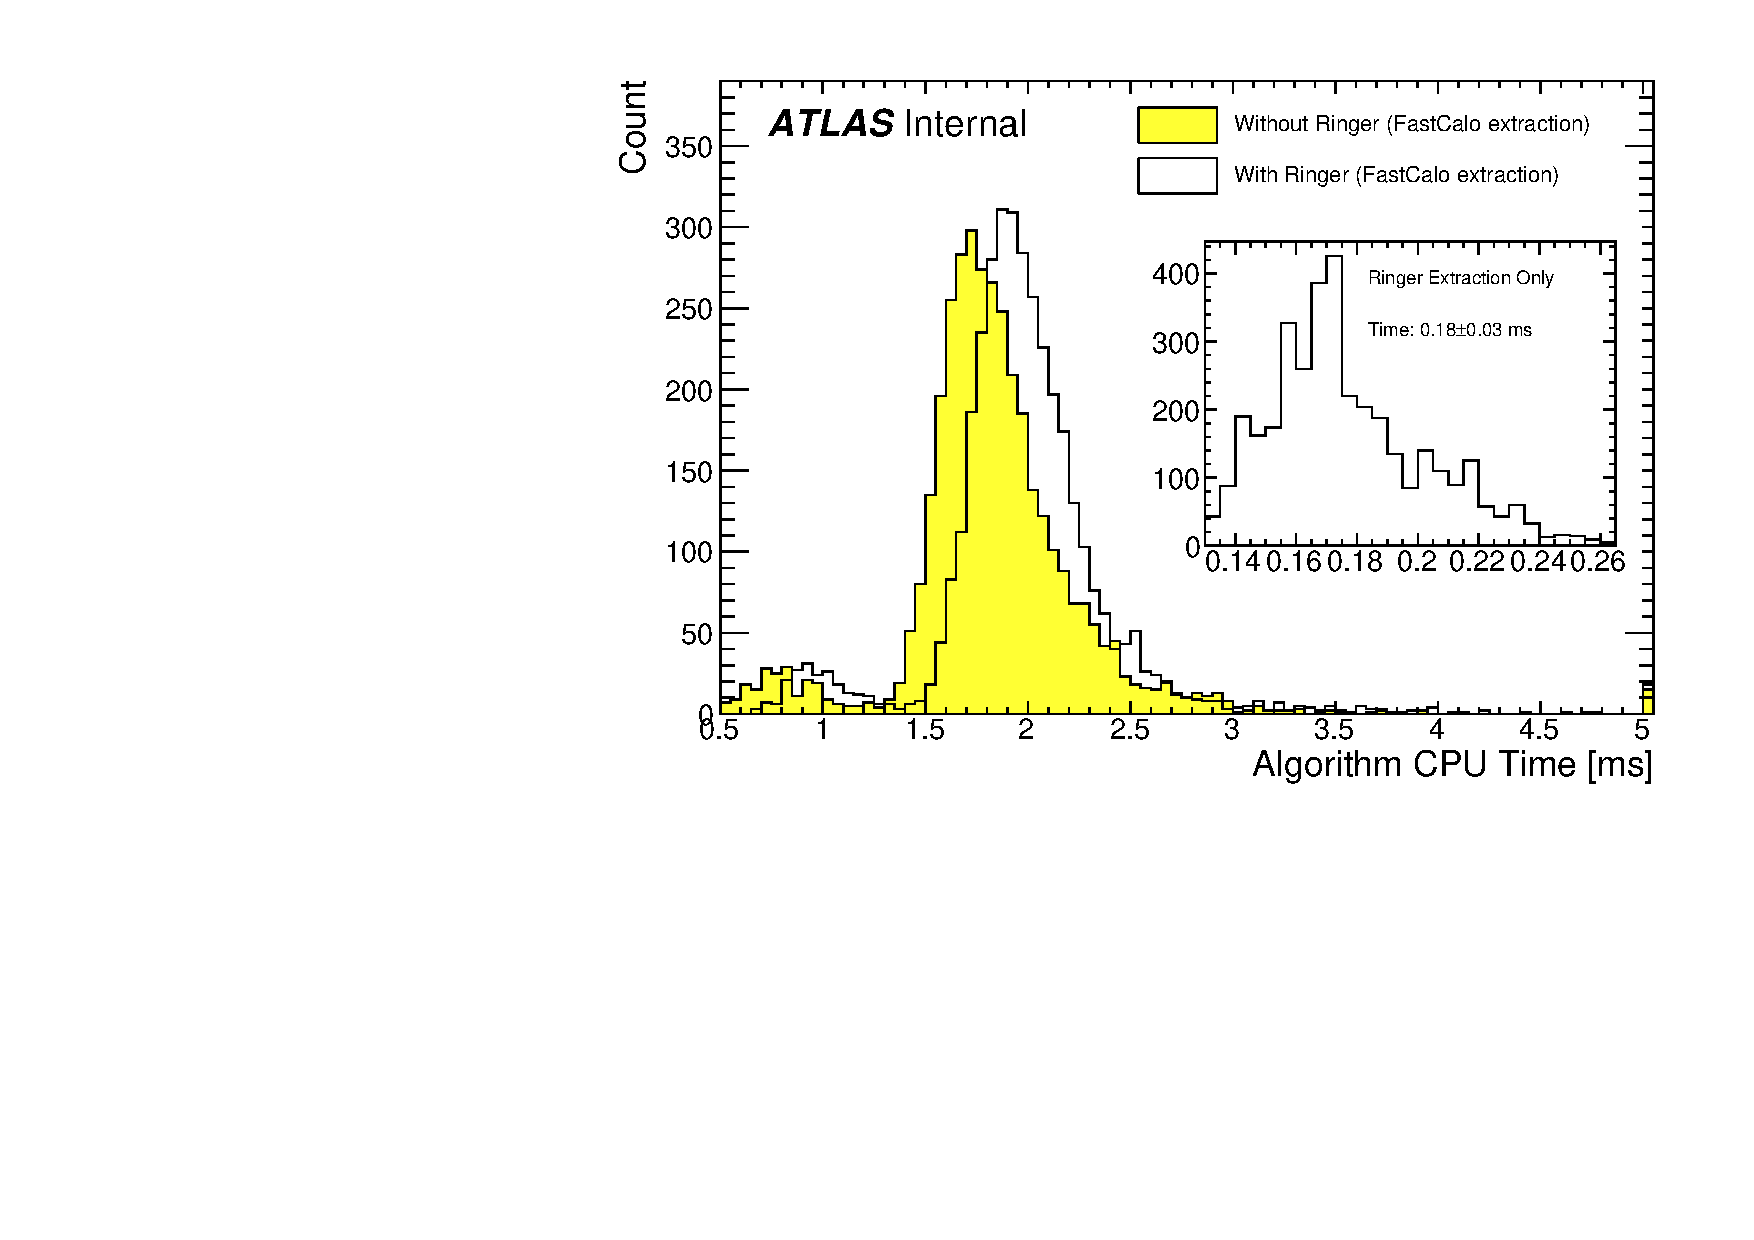
\includegraphics[width=.7\textwidth]{sections/05_analysis/figures/EgammaFex_TotalTime}
	\centering
	\caption{\label{fig:fastcalo_fex_time}
		Total CPU time per event for the feature extraction algorithms in the \fastcalo step of electron triggers with (white) and without (yellow) \rnn{} using EB events ($\avgmu=45$ peak). Detail on the right shows the CPU time of the ring variable extraction.  
	}
\end{figure}

\begin{figure}[h!tb]
	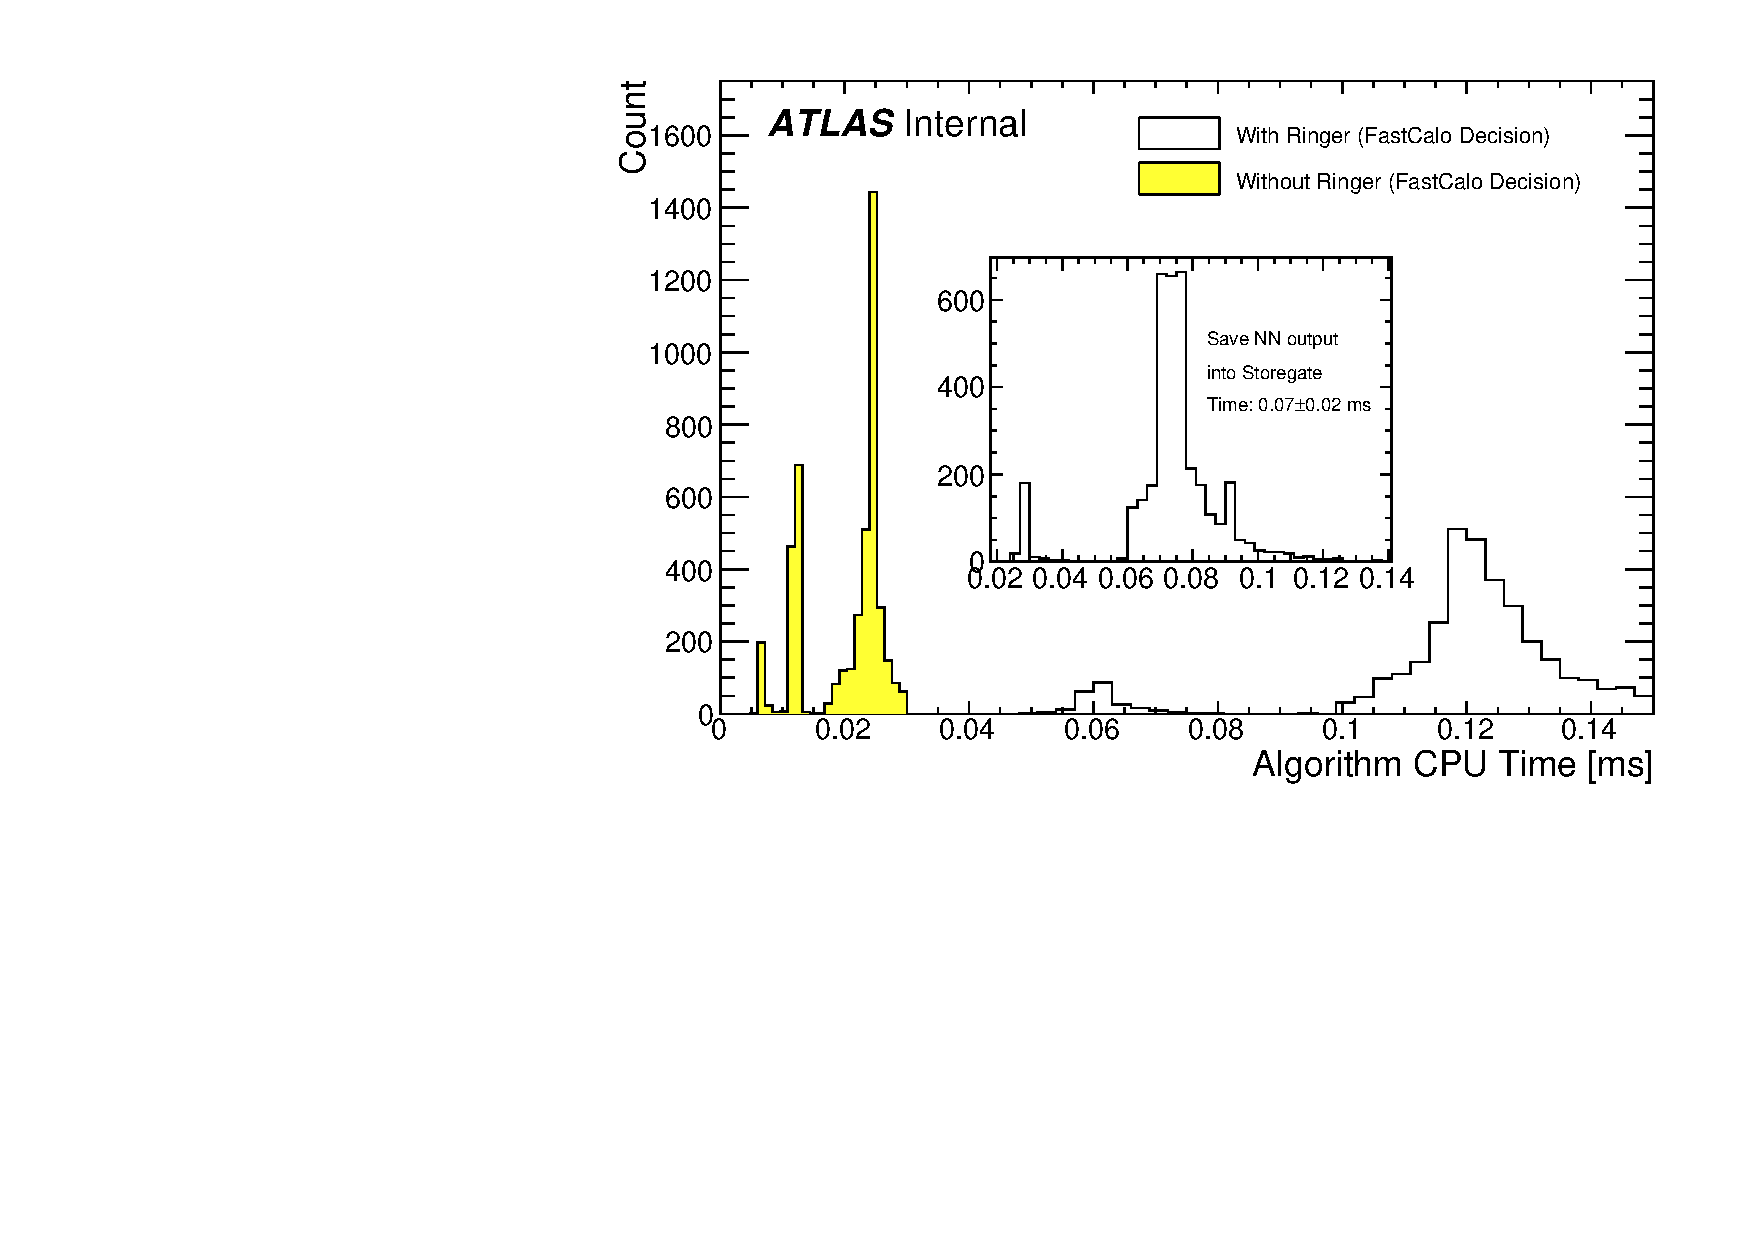
\includegraphics[width=.7\textwidth]{sections/05_analysis/figures/EgammaHypo_TotalTime.pdf}
	\centering
	\caption{\label{fig:fastcalo_hypo_time}
		Total CPU time per event for the hypothesis testing algorithms
		in the \fastcalo step of electron triggers with (white) and without (yellow) \rnn{} using EB events ($\langle \mu \rangle = 45$ peak). The center histogram represents the CPU time to store the \rnn{} output in persistent file format.}
\end{figure}

A multi-modal structure can be observed in the feature extraction distributions
of both trigger configurations, which is associated to the algorithm
for retrieving the EM2 cells and building related shower shape
variables\footnote{The three peak structure comes from the raw data conversion.
	Particularly, these are amongst the most-demanding contributions to
	the \fastcalo total CPU time.}. The computation of the ring variables, the only difference between the
triggers in the \fastcalo feature extraction, requires an additional average CPU time per
event of \SI{0.18 \pm 0.03}{\ms/\text{event}}. 
A less relevant contribution
comes from hypothesis testing, in which the ring variables are normalized, the
discriminant is computed, compared to the selection requirement and stored into the persistent file format\footnote{For Run-3 this step has been removed as a way to reduce the CPU time at \fastcalo step.} persistent format. 
Specifically, \rnn{} hypothesis testing is considerably more demanding
, up to \SI{0.14}{\ms/\text{event}}, mostly due to the time 
to store the neural network output \SI{0.07 \pm 0.02}{\ms/\text{event}}, 
than the cut-based selection
(\SI{0.02}{\ms/\text{event}}), however small with respect to the feature
extraction values. 


Taking into account the referred values, the \rnn{} can require a
relative increase of up to \SI{50}{\%} in the \fastcalo{} CPU time per event
with respect to the trigger without \rnn{}\footnote{We expect the result to be
	dependent on the trigger configuration due to presence of pile-up. Reported
	results are for e17\_lhvloose\_nod0.}. Nonetheless, the \rnn{} contributes to
a more discriminant selection, allowing to reduce CPU demanding triggers
by reducing the processing of fake electron in the computationally demanding
subsequent steps as will be shown in the following subsection.

\FloatBarrier
\subsection{Estimated CPU Impact on the Lowest-Energy Threshold Unprescaled Single Electron Trigger}\label{top:cpu_e26}

The potential of saving CPU usage by
avoiding the computation of fake candidates with the \rnn algorithms was demonstrated using algorithms with the lowest-transverse-energy-threshold unprescaled single electron tight trigger. This trigger algorithm was executed with
%(tight criterion). We executed it with 
and without the \rnn{} algorithm using a dedicated node for processing.
In this measurement, we considered about 3,400 events from EB stream %of run
%327265 processed with} release AthenaP1,21.1.55. 
The \rnn{} algorithm provided an overall
\SI{60}{\%} reduction (\SI{30.72}{\milli\second} to \SI{10.36}{\milli\second})
in the CPU demands.


\section{Quadrant Analysis}\label{ssec:quadrant}

The Quadrant Analysis was developed to compare the decision of two classifiers. Given signal candidates and two classifiers, these are the possibilities: either both accept or reject the candidates or only one accepts the candidates. The four possible decision quadrants are evaluated from shower shape distributions.
In this approach, only data collected by the primary triggers whose selection is from its offline equivalent are considered\footnote{I.e., if a \tight{} trigger leg is being evaluated, we also apply \tight{} offline selection to the candidate.}.
Results in Section~\ref{top:quadrant_results} show
trigger selection performance using \tight{} requirement for the duplicated triggers during 2017.

\subsection{Results}\label{top:quadrant_results}



We begin the Quadrant Analysis with the variable \reta{} for being one of the
most electron-jet discriminating variables employed in the likelihood
algorithm~\cite{aaboud2019electron}. As shown in Figure~\ref{fig:quadrant_calo_variables_30GeV_eta}, the disagreement, obtained by summing the cases accepted only by a single trigger between both triggers, is small and bounded for most cases at 1\% level for the coverage of all calorimetry variables. 
This behavior is also observed for \et{} slices. 
One should note that the working points of both triggers are not  exactly the same, although the \rnn{} aimed at keeping the same signal efficiency as being achieved by the cut-based strategy and was operating as desired.  
%Thus, much of the differences reflect this difficulty. 
In other words, 
%One should note that the integral of the single trigger cases is related to the limitation in the precision of setting the working point of both triggers to be exactly the same. In other words, 
the difference in height of the blue and red profiles in Figure~\ref{fig:quadrant_calo_variables_30GeV_eta} is mainly due to the small differences in efficiencies between the two triggers.
From the operation, it was realized that such working point matching was better in the $0.6<\abseta{}<0.8$ region. Hence, comparison between profiles is simpler to be performed there.
%Hence, comparison between profiles is simpler to be performed in the $0.6<\abseta{}<0.8$, which exhibits very similar performance.

For all variables in this region, both triggers behave very similarly (see Figure~\ref{fig:quadrant_calo_variables_30GeV}), even if some slight shifts can be observed in few profiles. This is the case of \reta{} and \rphi{}, where the \rnn{} trigger is consistently collecting slightly more events in signal region, i.e. respectively with slight tighter showers in $\eta{}$ and $\phi{}$ in the EM2. The \rnn{} trigger behavior shows even lower effect in the \rhad{}, where tighter tails are observed, resulting in less electrons with 10\% to 30\% energy in EM1, 1\% to 2\% in EM3 and more than 4 GeV hadronic leakage. \eratio{} also shows a slight bias towards collecting more events in the signal region with the \rnn{} trigger. Interestingly, some few events are accepted by the trigger with \rnn{}, when $0.5<\eratio{}<0.7$. We suspect it to be due electrons resulting from premature showers with barycenter near the edge of two strips

\begin{figure}[h!]
\centering
\begin{subfigure}[c]{.49\textwidth}
\centering
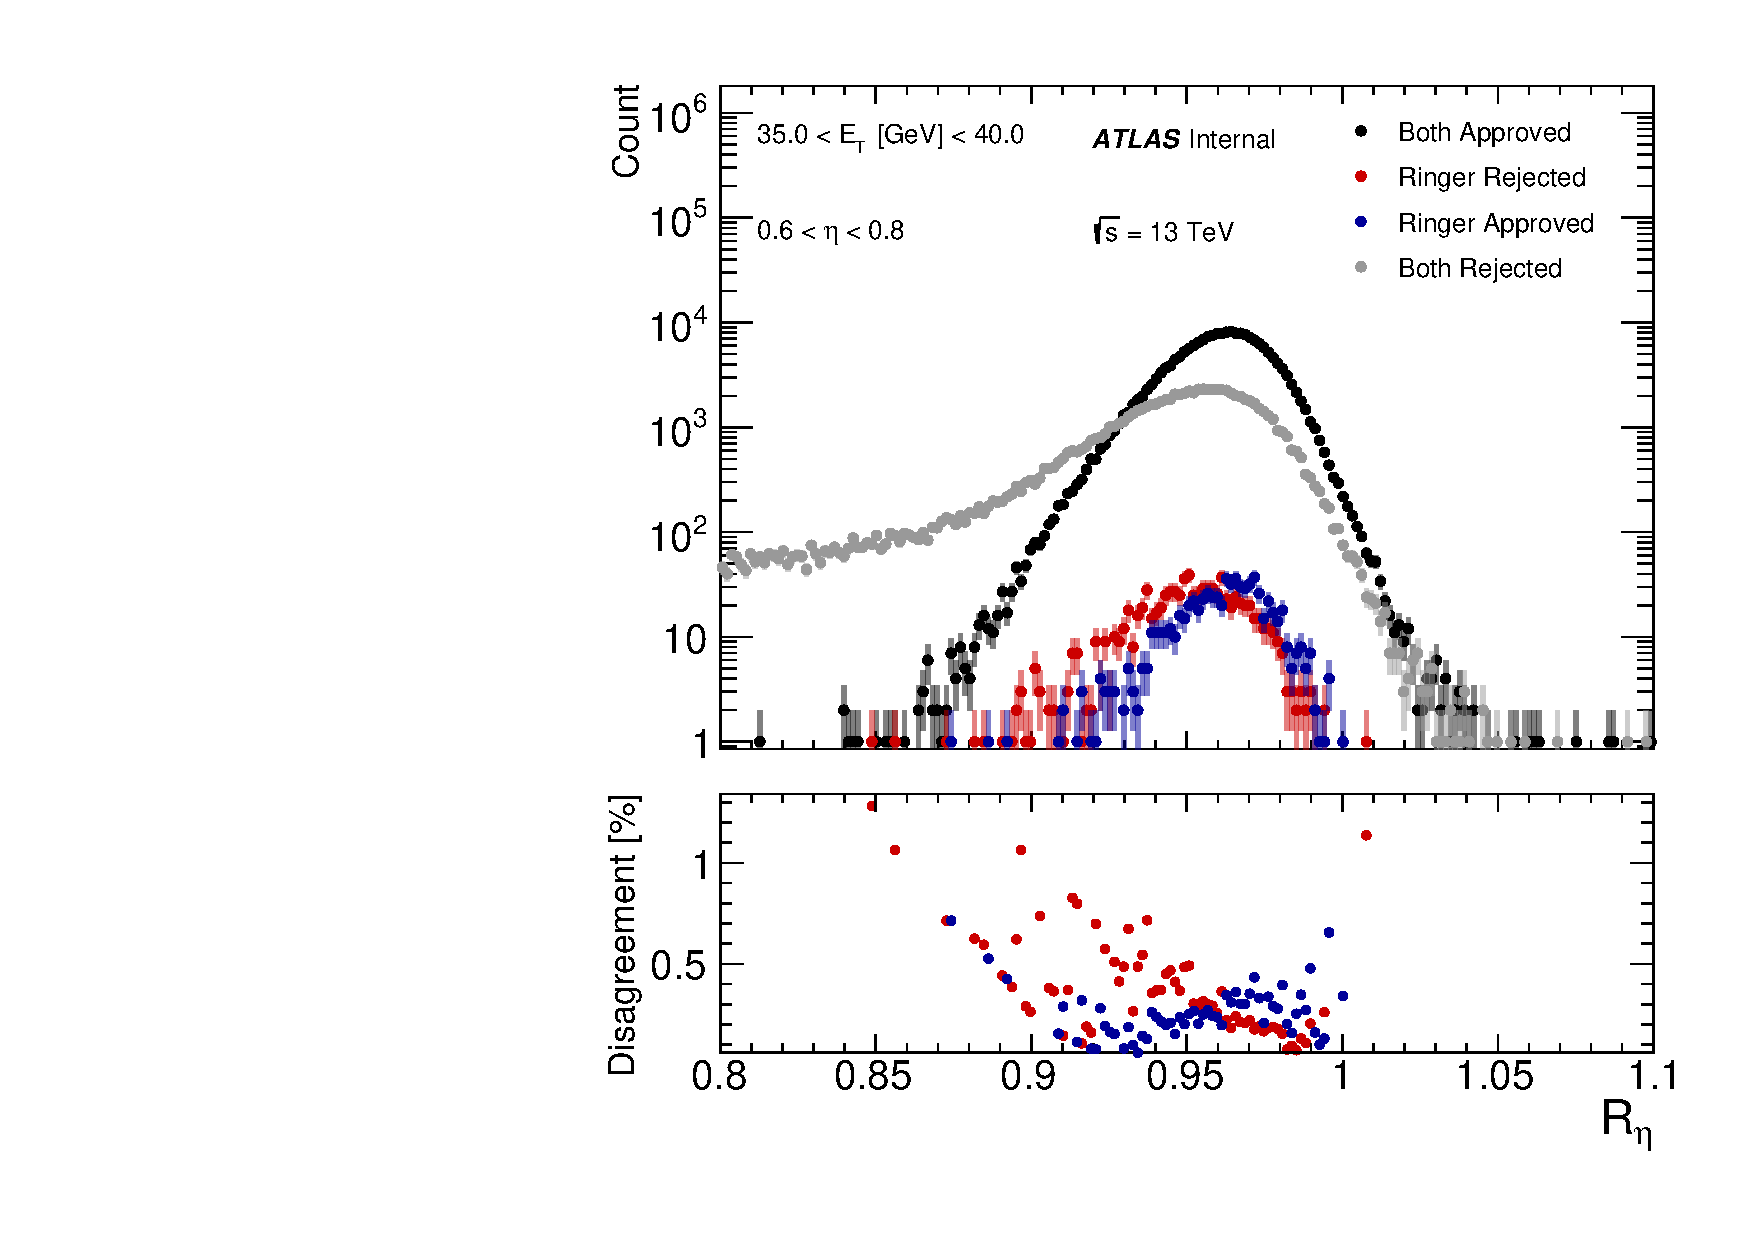
\includegraphics[width=\textwidth]{sections/analyses/figures/quadrant_plots/HLT_e28_lhtight_nod0_noringer_ivarloose_HLT_e28_lhtight_nod0_ivarloose_reta_et4_eta1.pdf}
\caption{}
\label{fig:quadrant_calo_variables_30GeV_eta}
\end{subfigure}
%\hfill
\begin{subfigure}[c]{.49\textwidth}
\centering
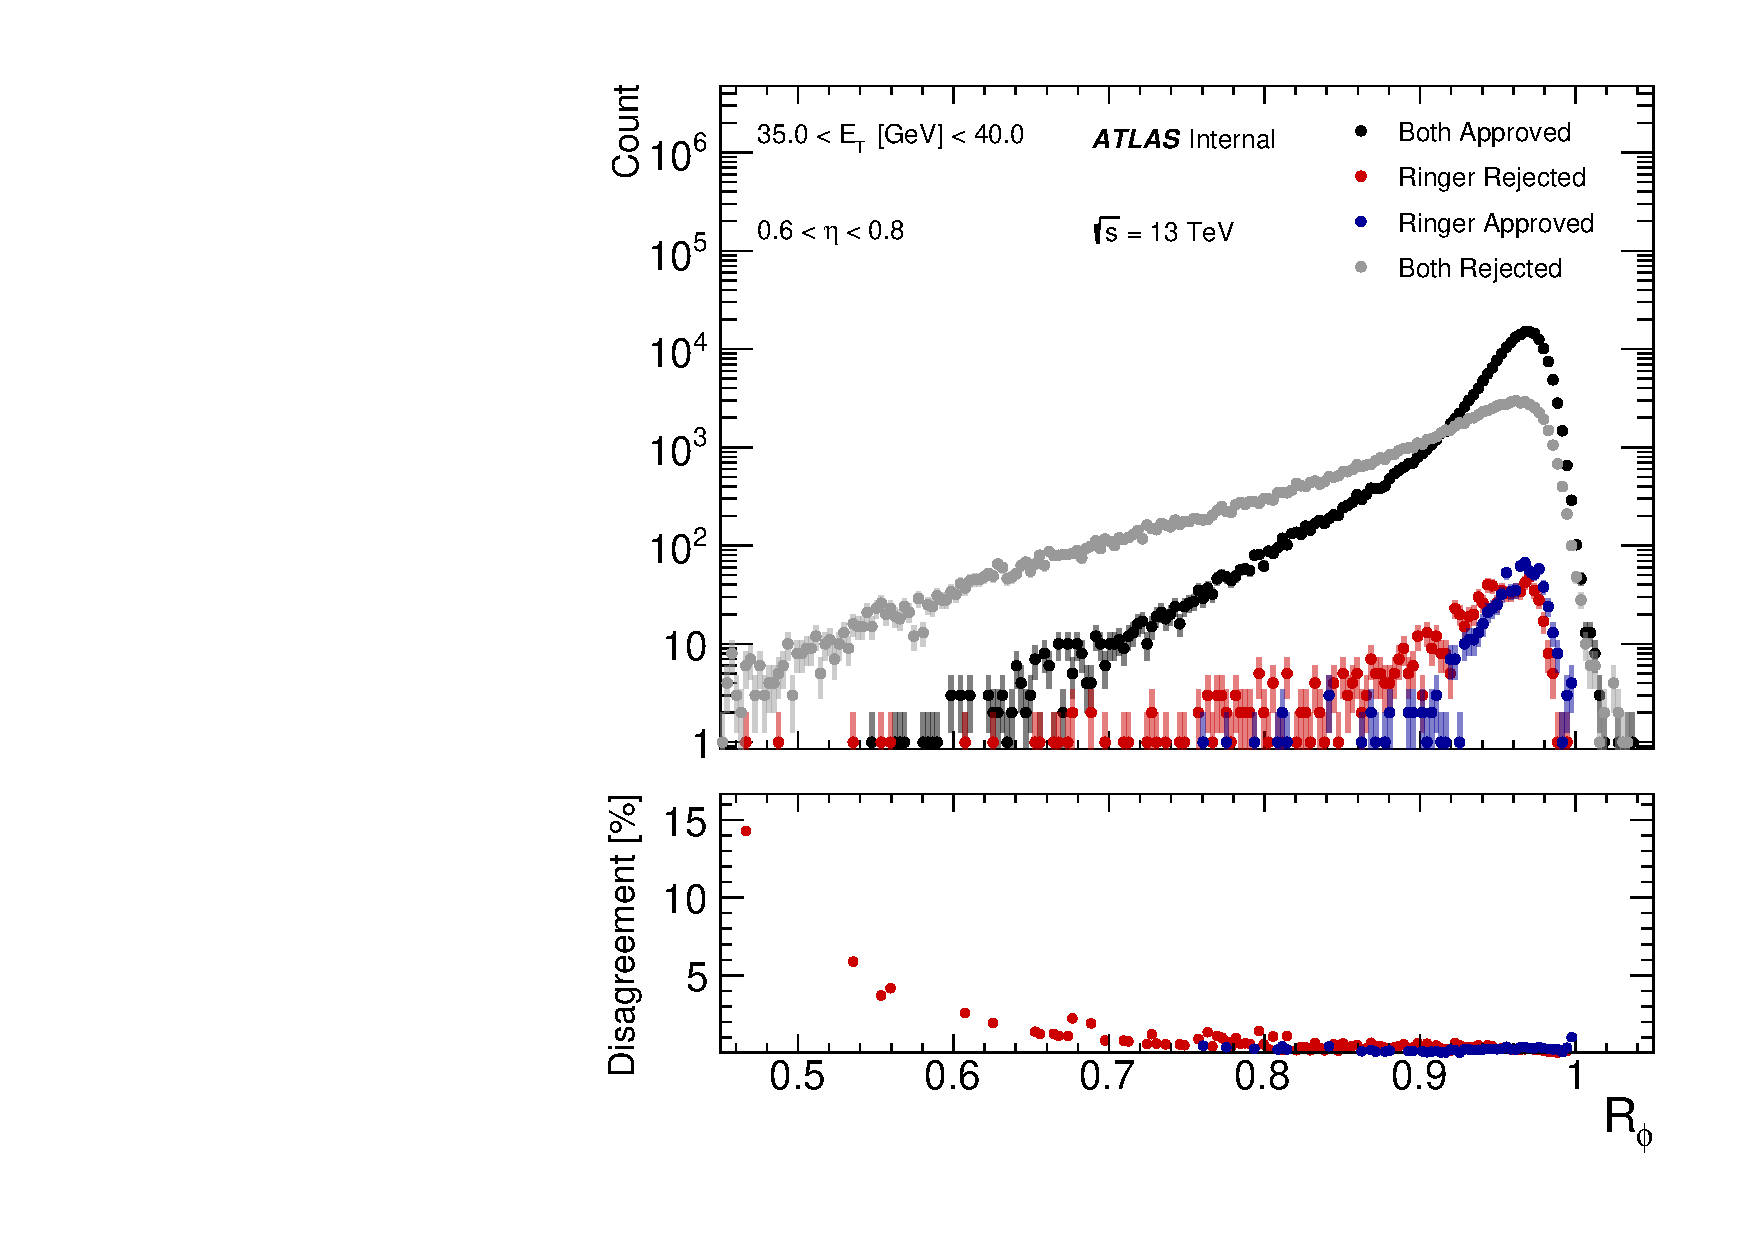
\includegraphics[width=\textwidth]{sections/analyses/figures/quadrant_plots/HLT_e28_lhtight_nod0_noringer_ivarloose_HLT_e28_lhtight_nod0_ivarloose_rphi_et4_eta1.pdf}
\caption{}
\end{subfigure} 
%\end{figure}
%\begin{figure}[p]\ContinuedFloat
\begin{subfigure}[c]{.49\textwidth}
\centering
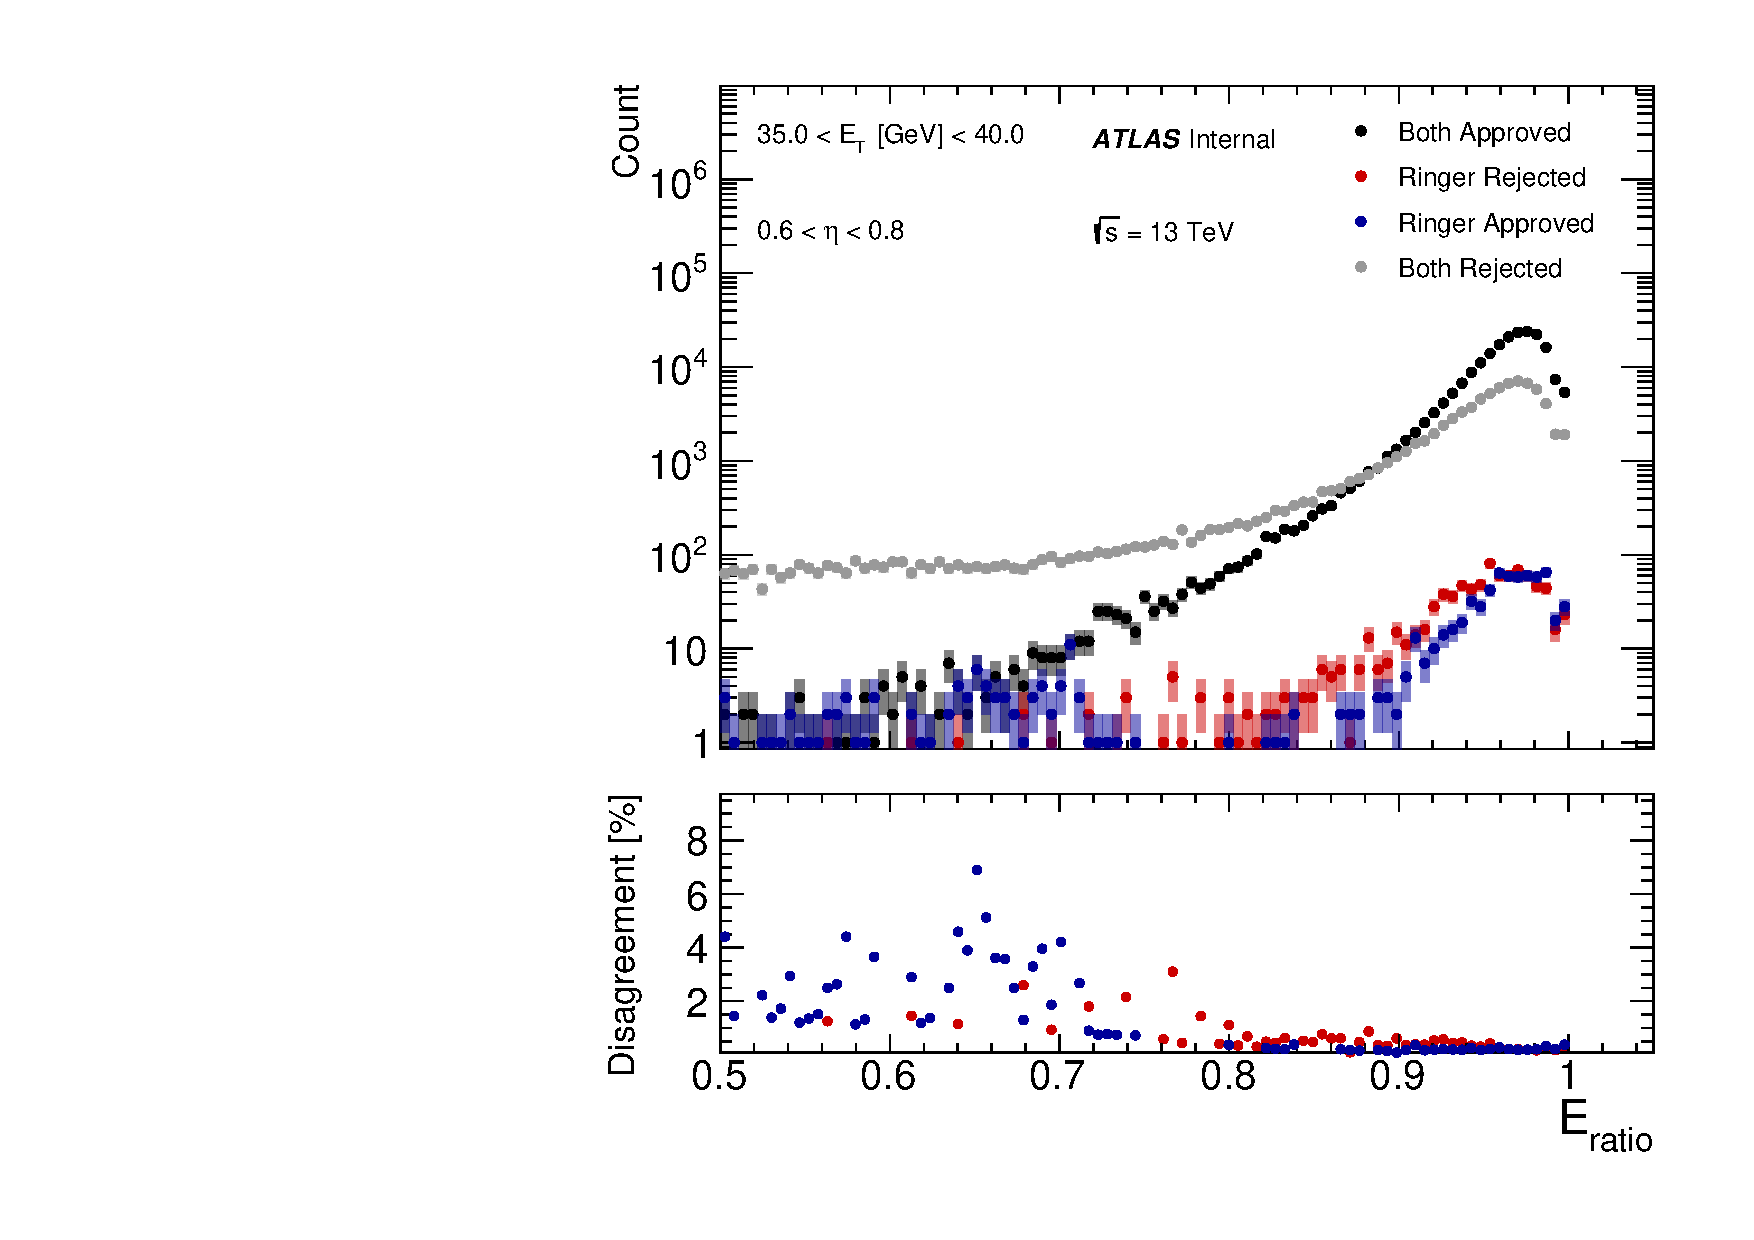
\includegraphics[width=\textwidth]{sections/analyses/figures/quadrant_plots/HLT_e28_lhtight_nod0_noringer_ivarloose_HLT_e28_lhtight_nod0_ivarloose_eratio_et4_eta1.pdf}
\caption{}
\end{subfigure}
\hfill
\begin{subfigure}[c]{.49\textwidth}
\centering
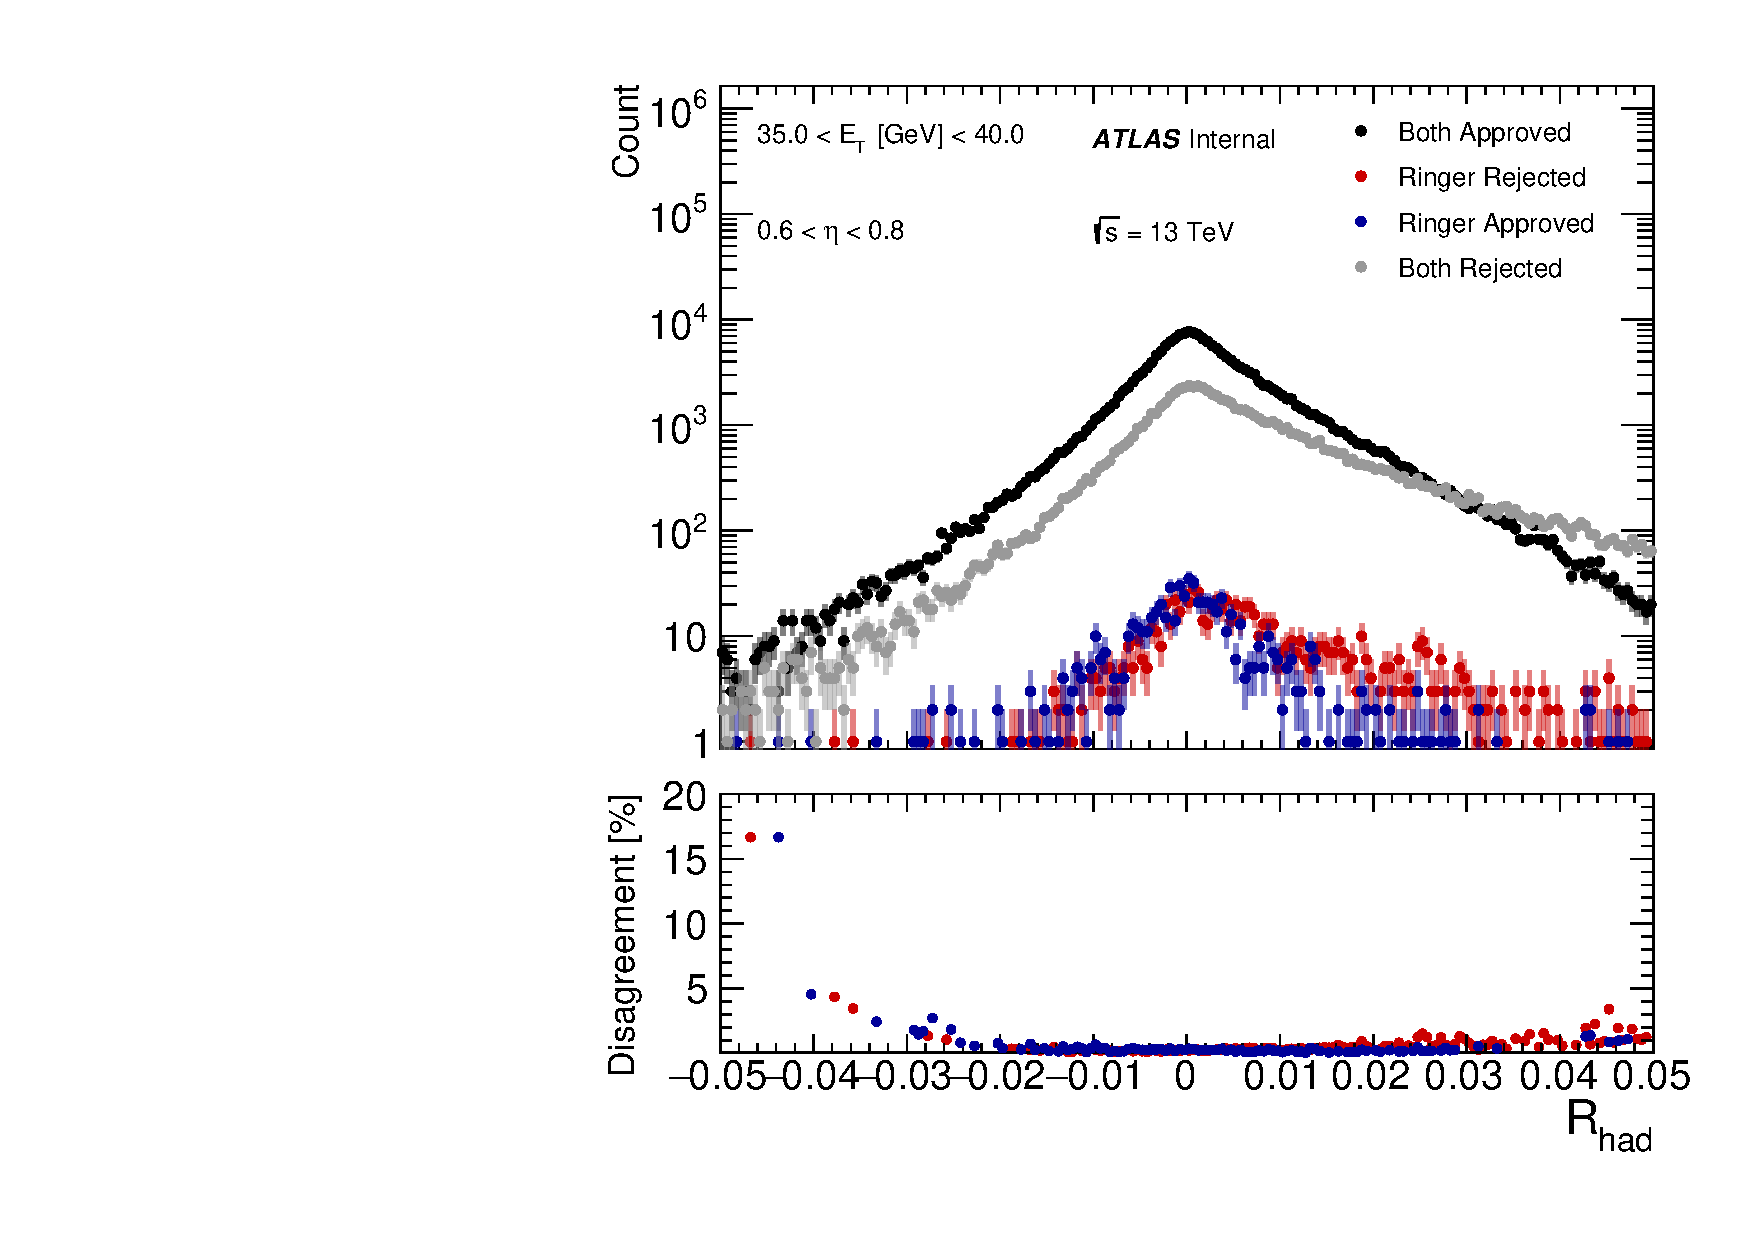
\includegraphics[width=\textwidth]{sections/analyses/figures/quadrant_plots/HLT_e28_lhtight_nod0_noringer_ivarloose_HLT_e28_lhtight_nod0_ivarloose_rhad_et4_eta1.pdf}
\caption{}
\end{subfigure} \\


\caption{\label{fig:quadrant_calo_variables_30GeV}
	Quadrant analysis plots for the main offline-reconstructed
	calorimetry variables employed in the
	likelihood and for the $0.6<\abseta{}<0.8$ and
	$30<\et{}~[\text{GeV}]<35$ slices. 
	The top pad in each figure shows the raw number of observations for the four mutually exclusive cases: both with and without \rnn{}
	triggered (black); triggered only with \rnn{} (blue); triggered only without \rnn{} (red); neither one triggered (gray). With the same color code, the bottom pad contains the percentage of each group with respect to the number of events selected by any trigger. The disagreement is defined by $(N_{blue}+N_{red})/(N_{blue}+N_{red}+N_{black}+N_{gray})$.
}
%Quadrant analysis plots for the offline-reconstructed
%calorimetry variables employed in the
%likelihood and \wstot{} for the $0.6<\abseta{}<0.8$ and
%$30<\et{}~[\text{GeV}]<40$ slices.}%
\end{figure}

Although similar behavior is shown for the other 
regions, the differences vary in strength in each \abseta{} region. As expected, 
the trigger does not show a dependent behaviour with ID variables, as shown in Figure~\ref{fig:quadrant_track_variables_30GeV} for $35<\et{}~[\text{GeV}]<40$, since the only distinction between them is the electron identification model operating in the \fastcalo{}.


\begin{figure}[h!tb]
%\centering
%\begin{subfigure}[c]{.49\textwidth}
\centering
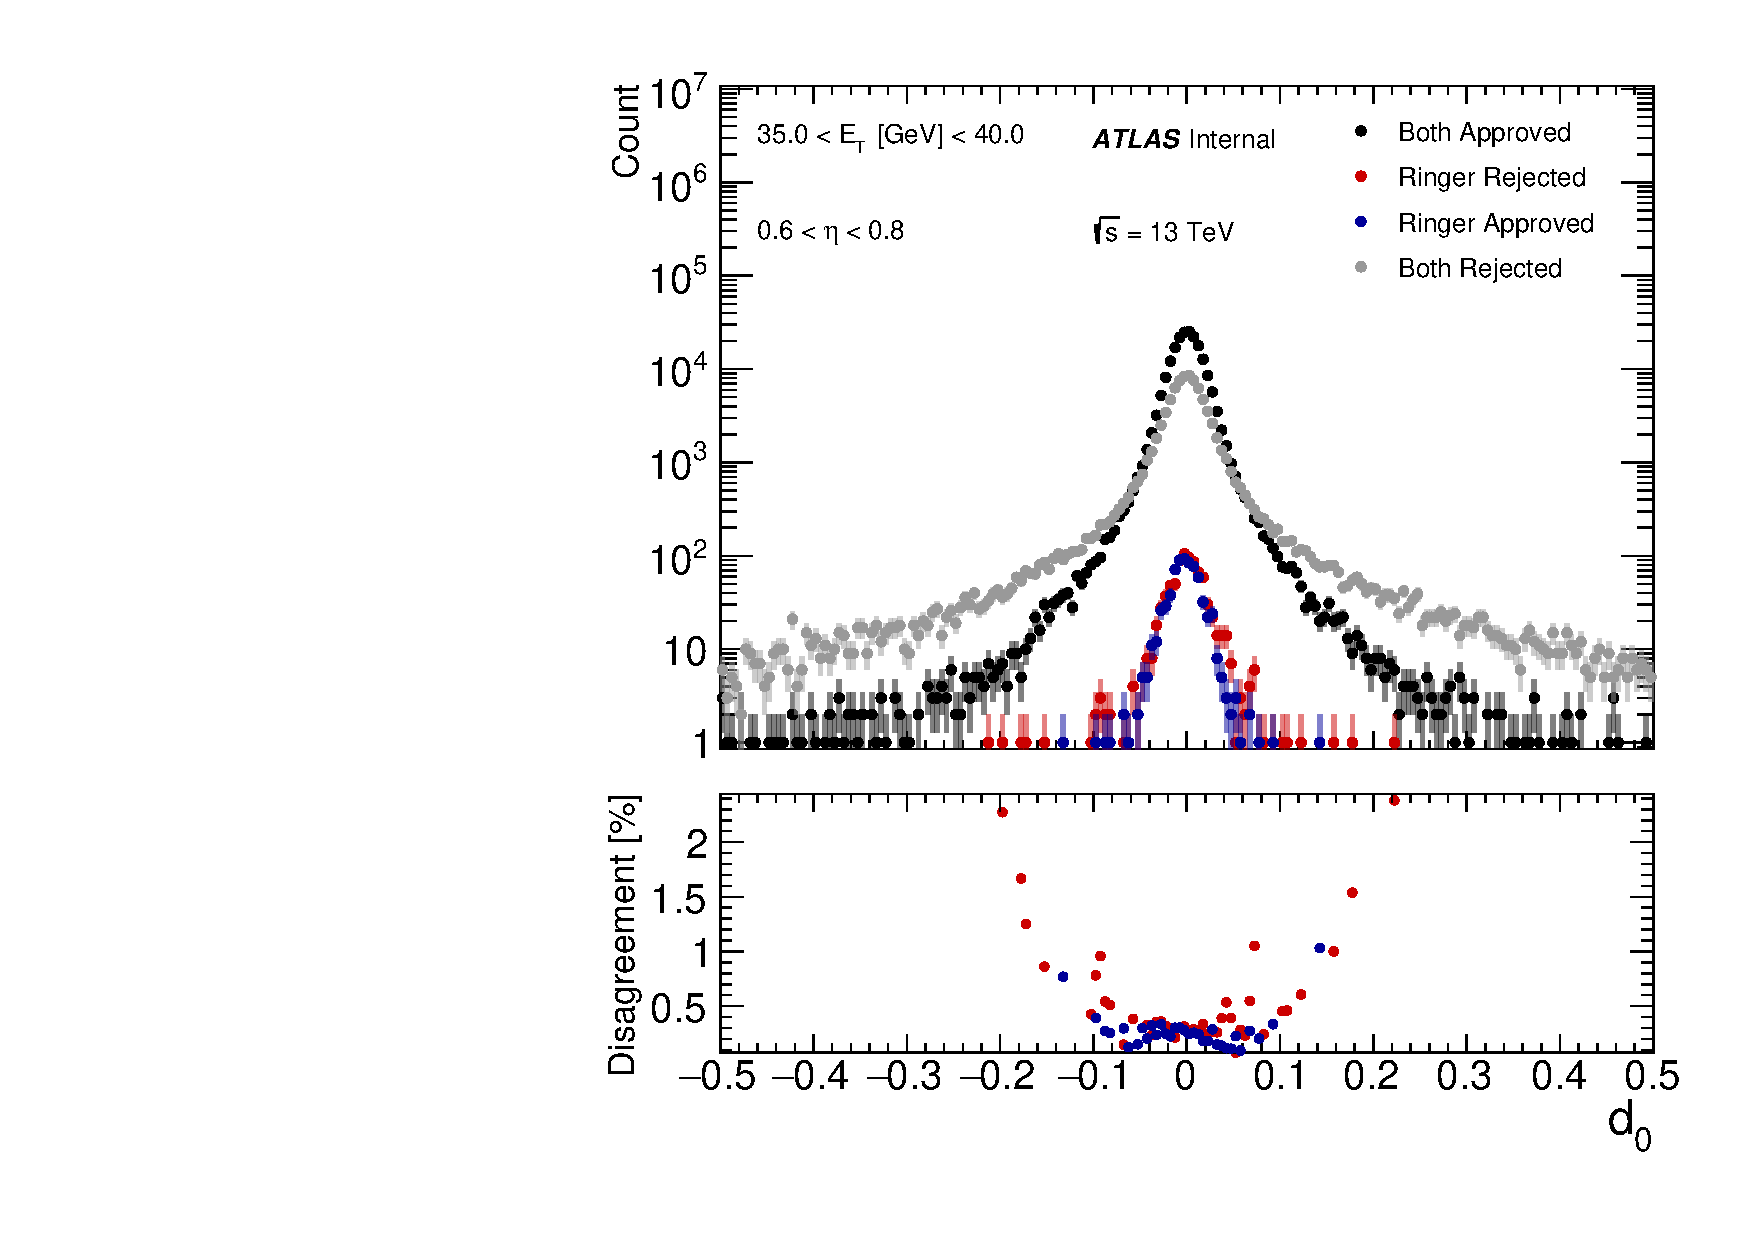
\includegraphics[width=.5\textwidth]{sections/analyses/figures/quadrant_plots/HLT_e28_lhtight_nod0_noringer_ivarloose_HLT_e28_lhtight_nod0_ivarloose_trackd0pvunbiased_et4_eta1.pdf}

\caption{\label{fig:quadrant_track_variables_30GeV}
Quadrant analyses plots for the offline-reconstructed ID variable $d_0$ employed in the
likelihood for the $0.6<\abseta{}<0.8$ and $35<\et{}~[\text{GeV}]<40$ slice. The variable $d_0$ is defined as the transverse parameter of the impact point with respect to the collision beam.
}
\end{figure}






\FloatBarrier
\section[Homogeneity Tests]{Homogeneity Tests}\label{ssec:agreement}

In this 
analysis, the impact of using different triggers, \rnn{} and cut-based, on the likelihood algorithm is evaluated. This 
%analysis, we observe how the usage of the different triggers (from \rnn{} and cut-based algorithms) may impact the likelihood algorithm. This 
study requires a pair of duplicated triggers, composed by an $E_T > 28$ GeV isolated and Tight selection with and without the \rnn{}, operating online together. 
This analysis is performed using \Zee{} \tnp{} data, which were selected with the trigger requirement set to either one of the duplicated triggers for the tag, whereas the probe selection is invariably set to the offline \vloose{} criterion. This is the exact setup employed by ATLAS to derive the offline likelihood for electrons above \SI{15}{\GeV}. To benefit from the full 2017 statistics, data collected previous to the TS1 were also employed. In case the profiles are statistically identical, then it is expected that the \rnn{} trigger does not cause any relevant alteration in the derivation of the offline likelihood pdfs.  The statistical method for profile evaluation is described in Section~\ref{top:homogeneity_method} and the results are available in Section~\ref{top:agreement_homogeneity_results}.




\subsection{Method}\label{top:homogeneity_method}



The problem is approached based on homogeneity tests on histograms~\cite{homogeneity_test}, in order to check for (systematic) effects of the trigger configuration. It is based on a test originally developed by Pearson~\cite{pearson1911probability} and popularly employed in many fields beyond High Energy Physics (HEP), e.g. social sciences~\cite{wickens2014multiway} and health~\cite{ma2015homogeneity}, usually labelled as contingency or consistency tests.

In order to benefit from the test without having to customize it to the ATLAS particular analysis setup, we proceed the following way. First, we split data into two
statistically independent groups attempting to keep data taking conditions as
similar as possible by successively taking data to each group from small
consecutive periods. Ideally, it would be desired to split data using luminosity
blocks for achieving nearly the same conditions. However, technical limitations
constrained the period to larger time scales, hence allowing the test to
indicate that the two groups are originating from different populations due to
confounding variables. 
Either way, it does not affect the goal of this assessment. By comparing the p-values of the two groups, we can evaluate how the different configuration affects the likelihood of the profiles to be drawn from the same distribution. If the p-values\footnote{The p-value here is defined by: $P-value \approx f(x, k) = \frac{1}{2^{k/2}\Gamma(k/2)}x^{k/2 -1}e^{-x/2}$} have negligible fluctuations with respect to the values obtained by the tests comparing the same triggers, then the systematic effect in the profiles is negligible with respect to half\footnote{Once each group is using nearly half of the integrated luminosity.} of the statistics available.



To provide a better insight on possible distortions, the corresponding $\chi$
individual contributions of each group are computed allowing them to freely
oscillate through the positive and negative axis with

\begin{equation}
  \chi_{i,j}^{s} = \frac{(r_{i,j} - b_{i,j})}{\sqrt{b_{i,j}}},
  \label{eq:signed_chi}
\end{equation}

\noindent where $r_{i,j}$ ($b_{i,j}$) is the number of observations collected by
the trigger with (without) \rnn{} in $j$th histogram bin and in the $i$th
$\et{}\times\abseta{}$ region.


\subsection{Results}\label{top:agreement_homogeneity_results}




Regardless of the trigger configuration, the p-values of the homogeneity tests between the two groups result in similar values. In other words, the fluctuations in the profiles are mainly dominated by statistical fluctuations, with no sign of systematic effects due to the trigger configuration. Similar behavior is observed for the ID and calo-ID variables. In Figure~\ref{fig:groups_homogeneity_calo}, we show the residuals when considering the histogram obtained with data collected by the trigger without \rnn{} for the first arbitrary group as a reference. The residuals are dominated by statistical fluctuations, which are within the expectations from homogeneity hypothesis for most variables and regions.


\begin{figure}[b]
\begin{center}
\begin{subfigure}[c]{.48\textwidth}
\centering
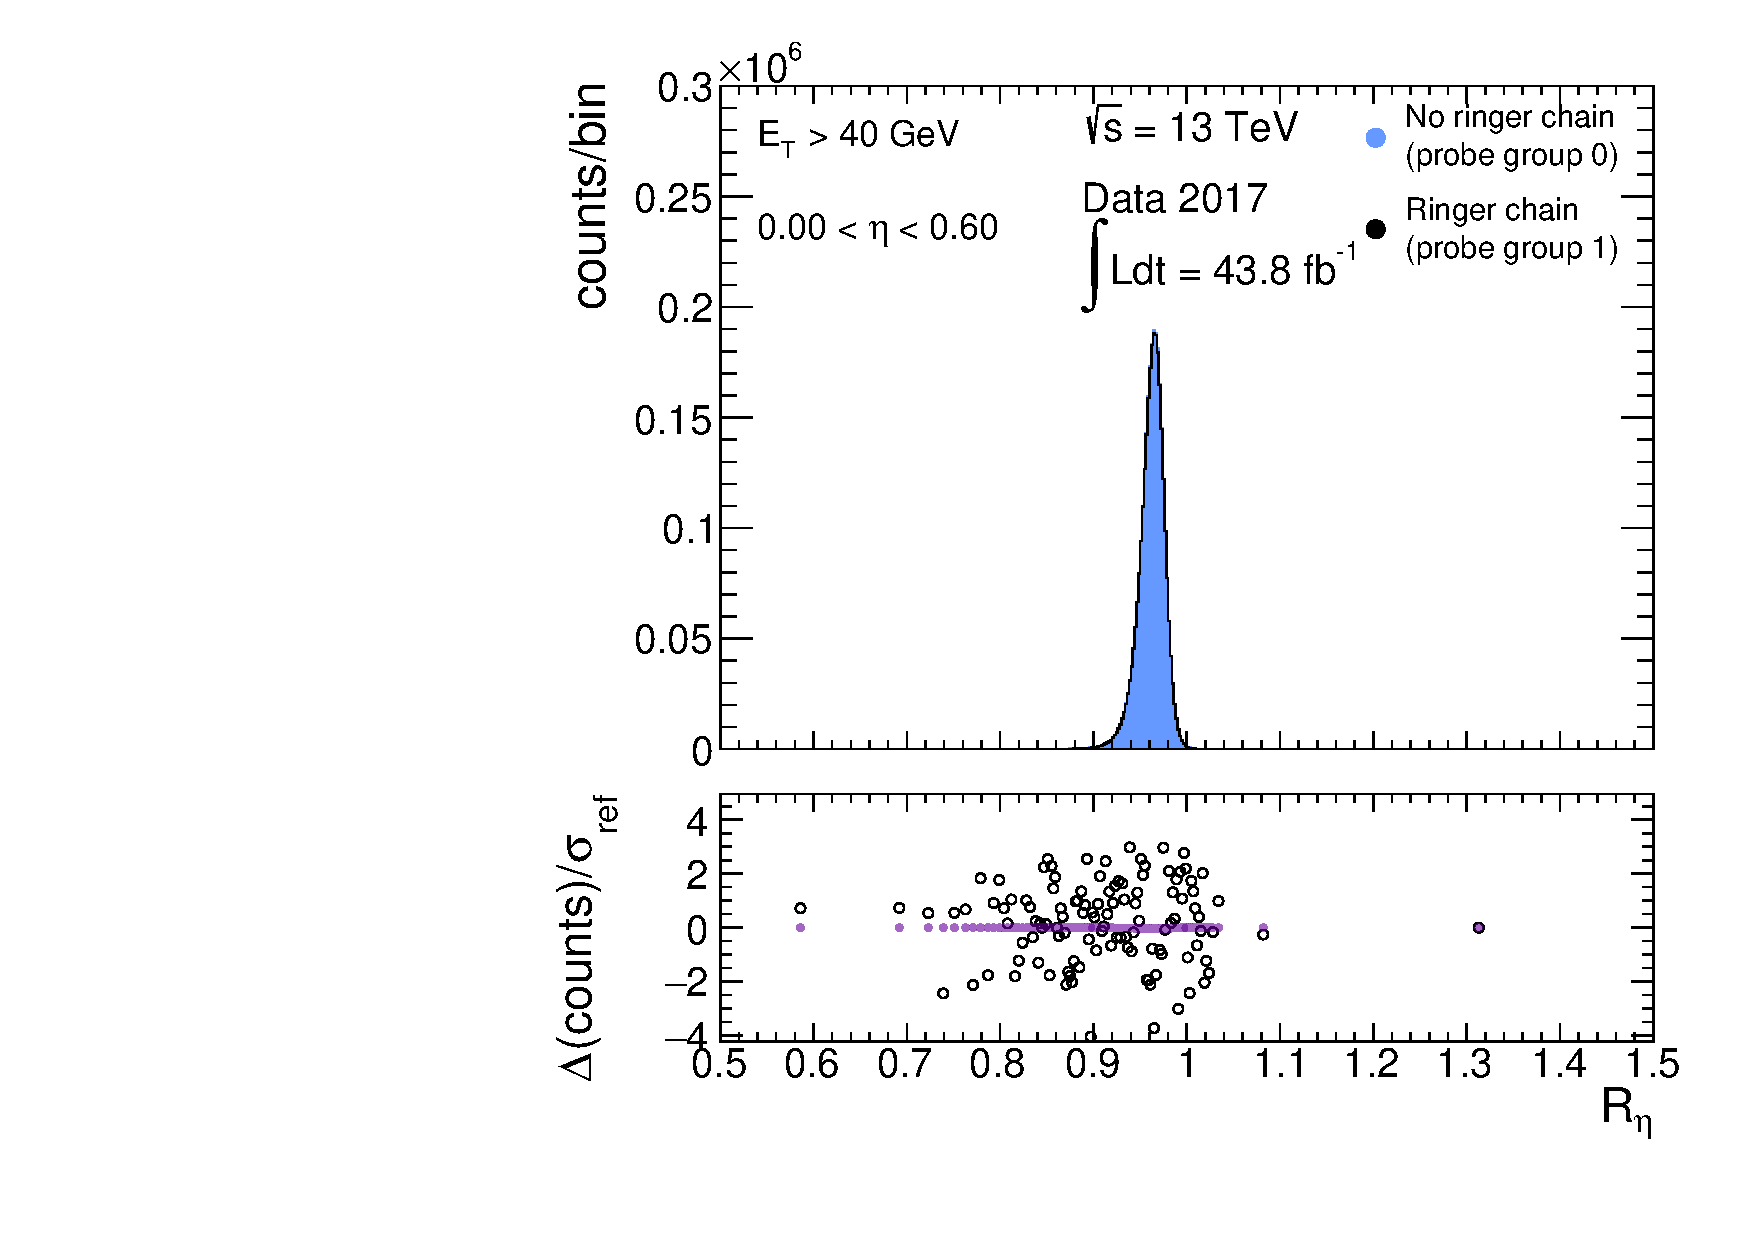
\includegraphics[width=\textwidth]{sections/analyses/figures/noAdjustment/el_reta_et40eta0_00_sigma_base_new.pdf}
\caption{}%

\end{subfigure}
\hfill
\begin{subfigure}[c]{.48\textwidth}
\centering
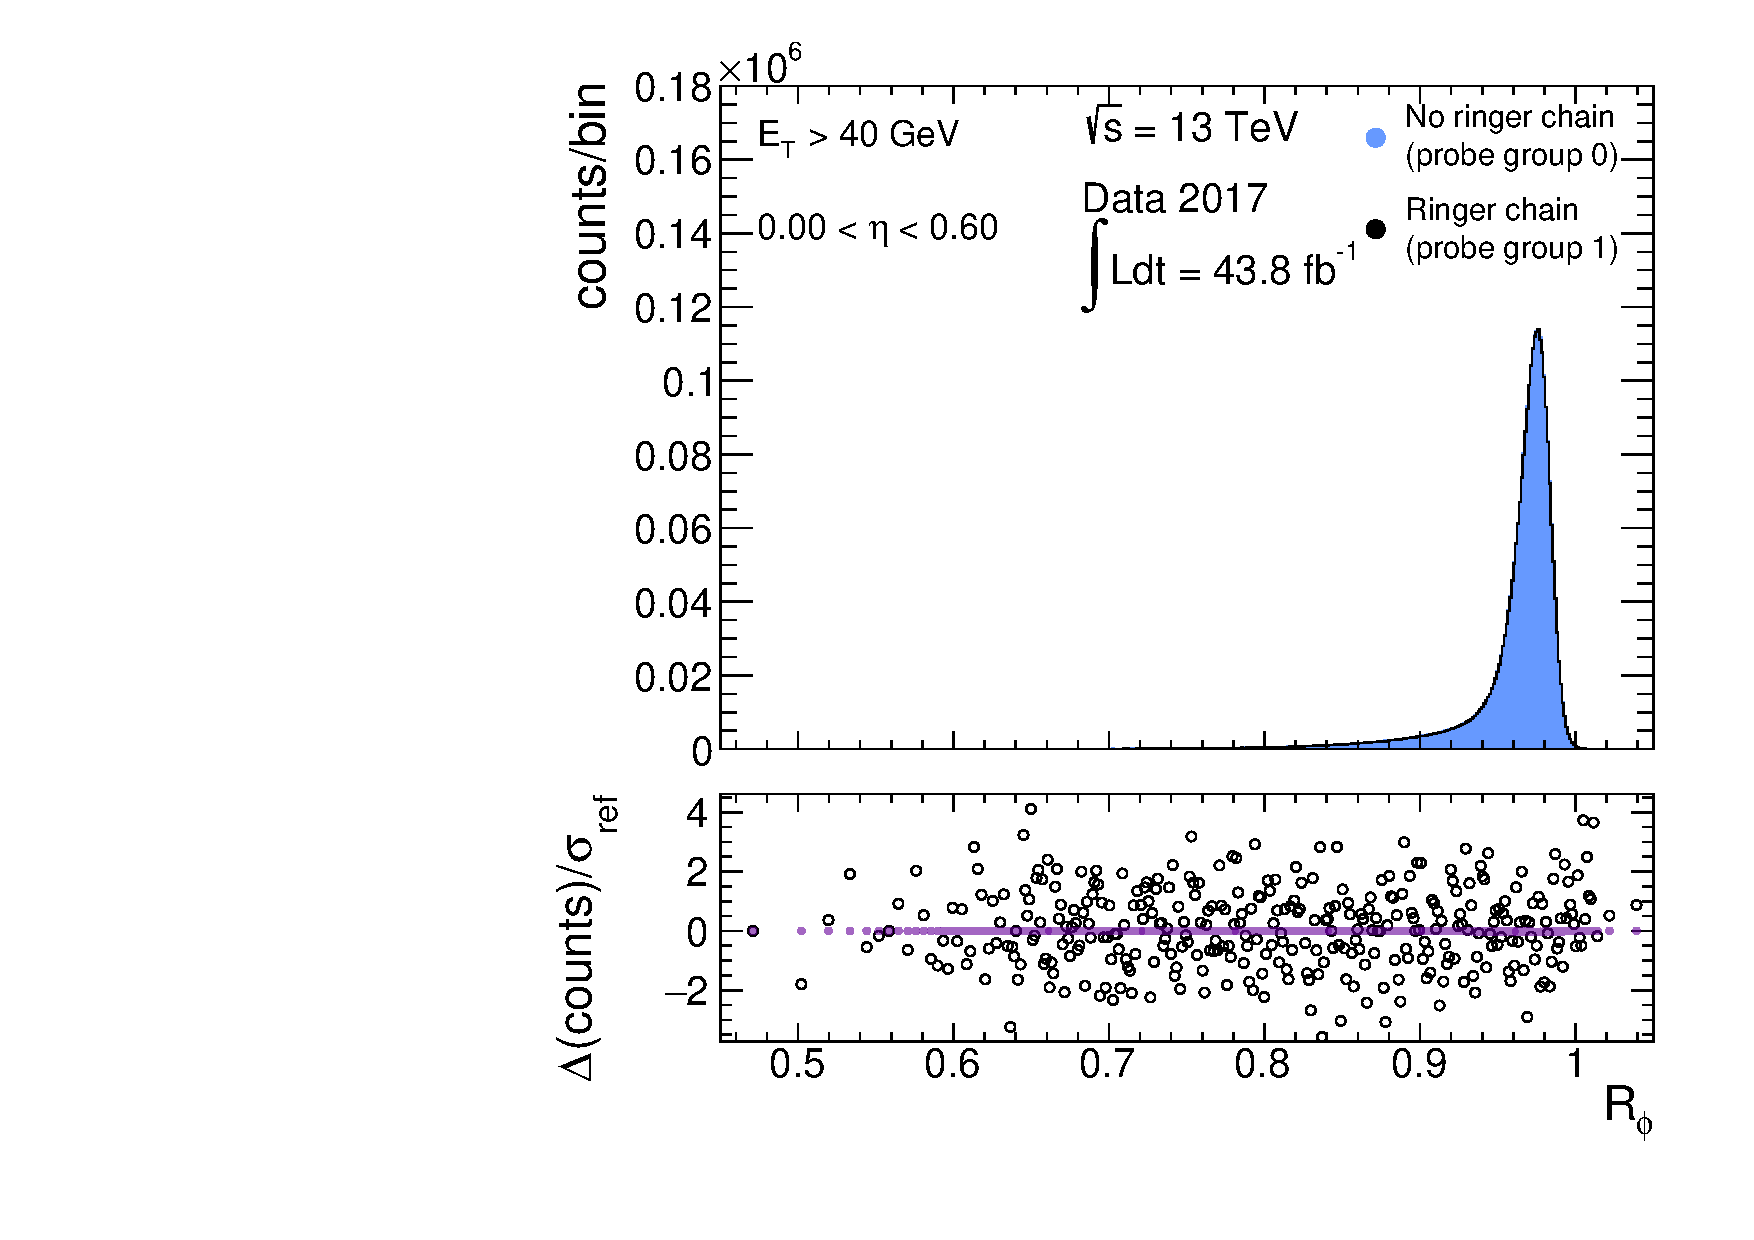
\includegraphics[width=\textwidth]{sections/analyses/figures/noAdjustment/el_rphi_et40eta0_00_sigma_base_new.pdf}
\caption{}%

\end{subfigure} \\
\begin{subfigure}[c]{.48\textwidth}
\centering
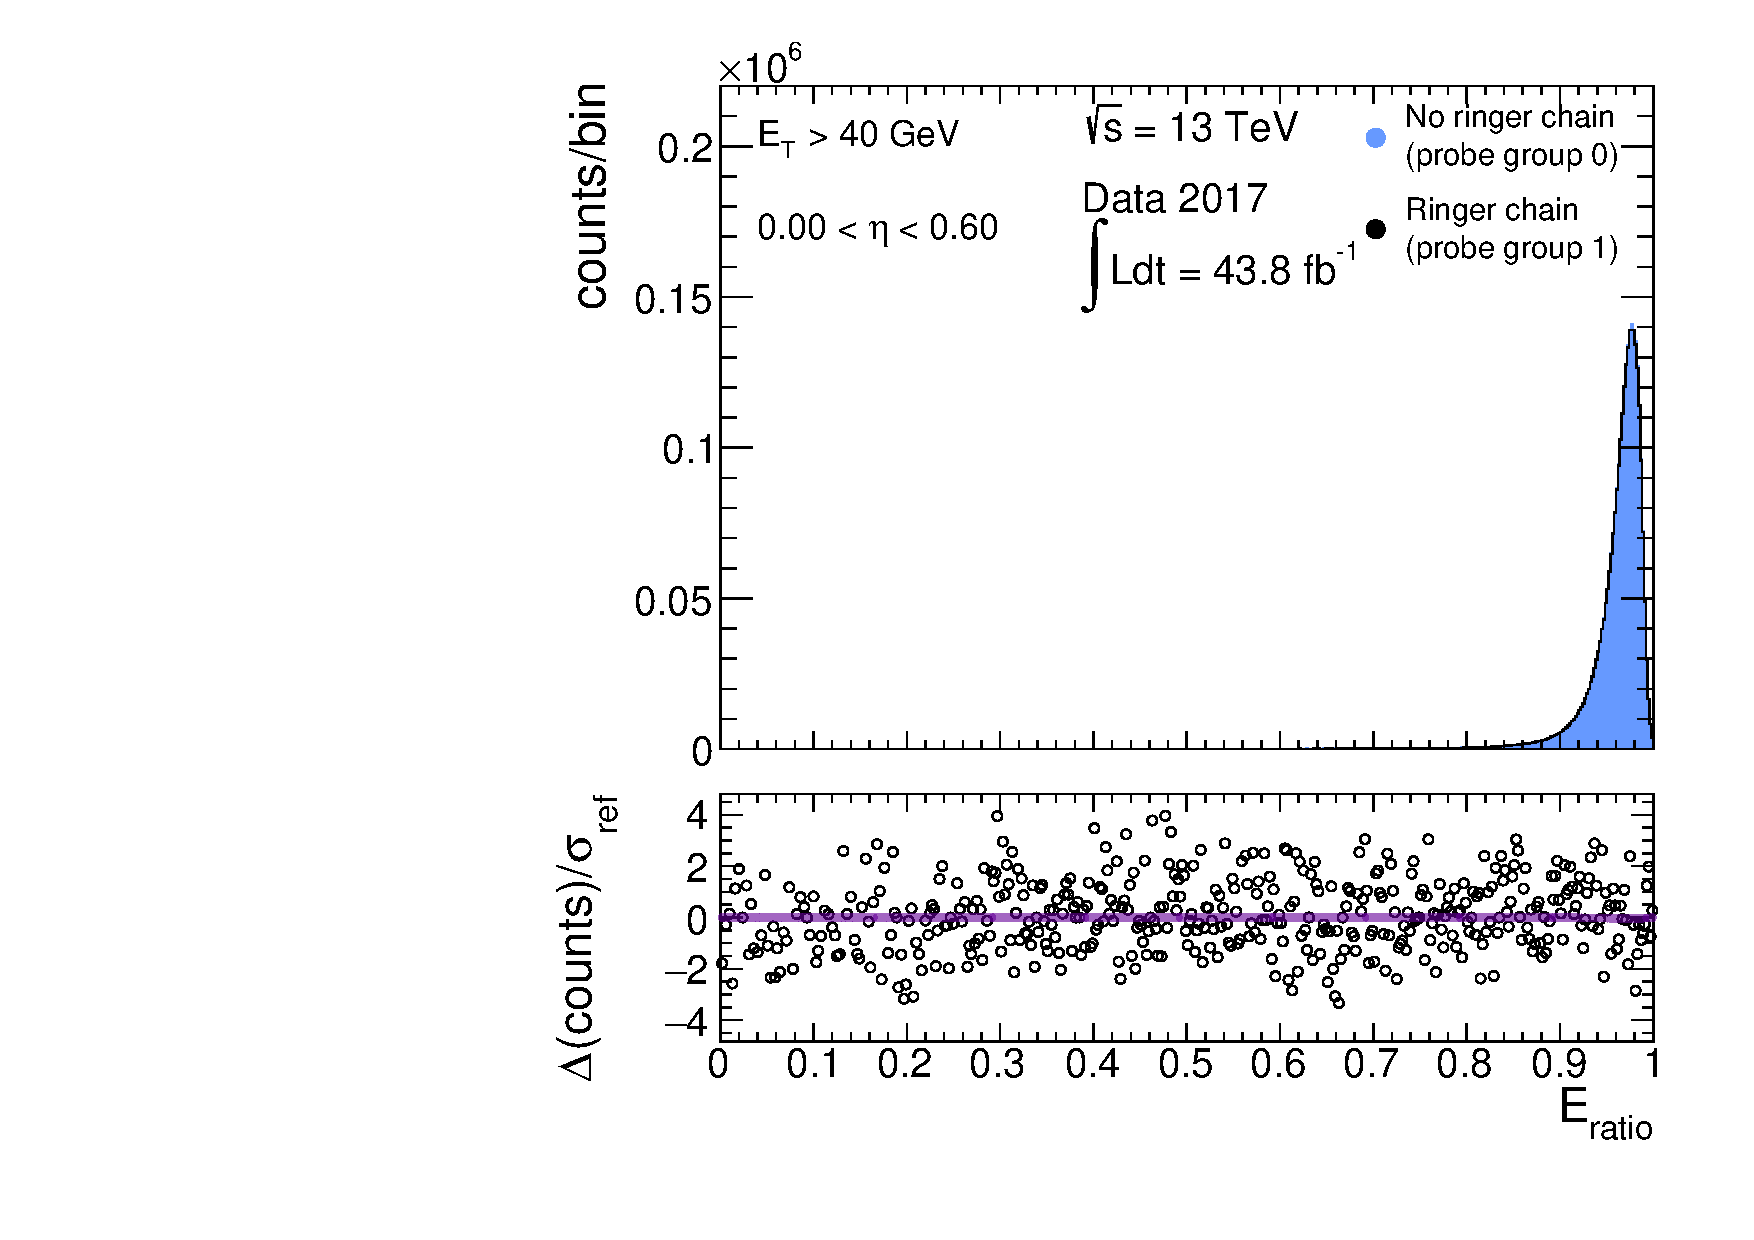
\includegraphics[width=\textwidth]{sections/analyses/figures/noAdjustment/el_eratio_et40eta0_00_sigma_base_new.pdf}
\caption{}%

\end{subfigure}
\hfill
\begin{subfigure}[c]{.48\textwidth}
\centering
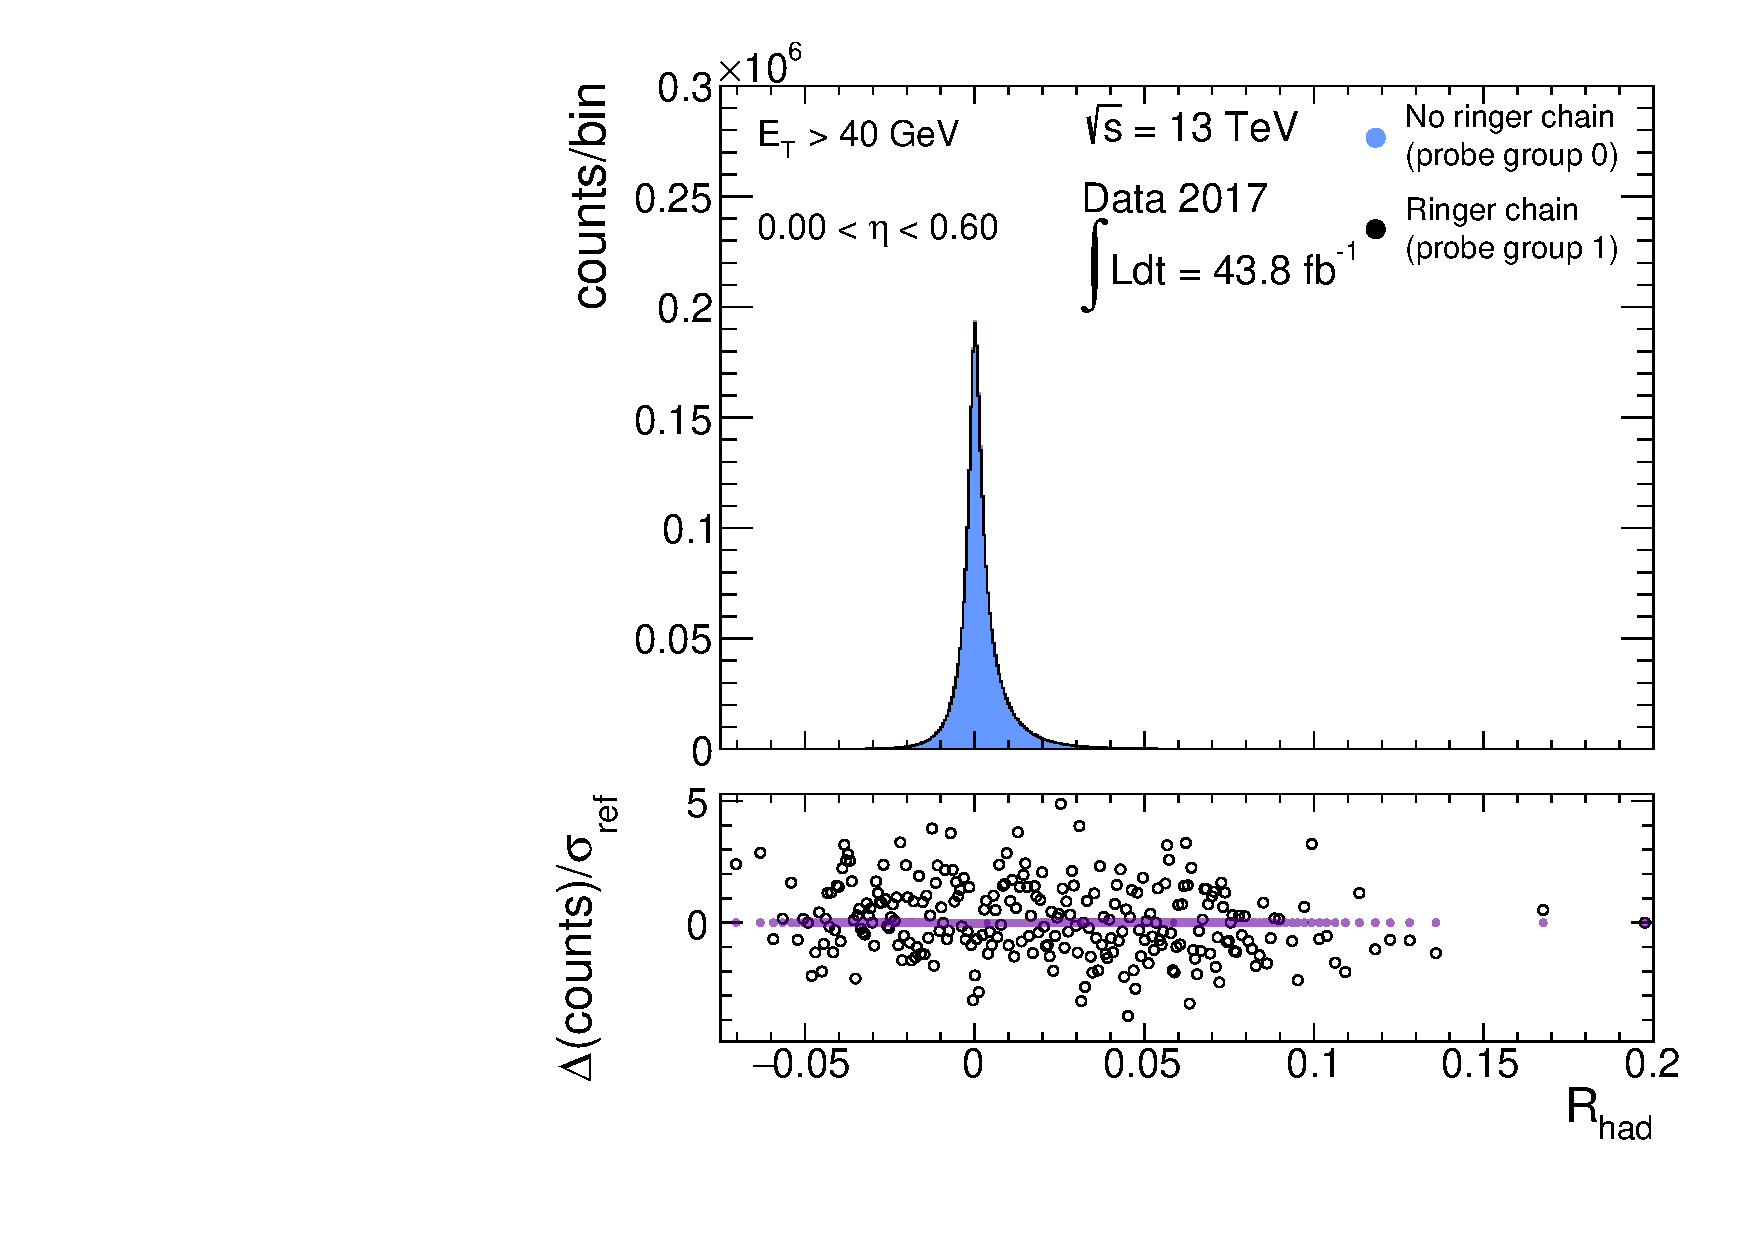
\includegraphics[width=\textwidth]{sections/analyses/figures/noAdjustment/el_rhad_et40eta0_00_sigma_base_new.pdf}
\caption{}%

\end{subfigure} \\
\caption{%
	Top: \reta, \eratio, \rphi, \rhad histogram profiles for the calorimetry variables employed in the offline likelihood in the $\et>\SI{40}{\GeV}$ and $0.00<\abseta{}<0.80$ regions using data collected by
	triggering without \rnn{} in the first arbitrary data group
	(blue area) and data collected by triggering with \rnn{} in the second
	arbitrary data group (black line).  Bottom: residual contributions using as
	statistics $\chi^s$ (equation~\ref{eq:signed_chi}, in black) and the expected
	model for no distortion given by the $\chi^s$ residuals w.r.t.\@ the
	reference.
}%
\label{fig:groups_homogeneity_calo}
\end{center}
\end{figure}%


\FloatBarrier
 % ok
\chapter{Conclusion and Perspectives}\label{sec:conclusion}
%-------------------------------------------------------------------------------


% Comparison with standard strategies
The \rnn{} brings an innovative design for electron selection based on
calorimetry information. By alleviating the implicit requirement of conceiving
variables to exploit individual properties of the particle interaction process, it introduces 
more general variables exploiting the process natural symmetries. With the
ambition to comply with specific trigger system demands, the feature extraction
of concentric ring energy sums provides an efficient description, which is quickly derived
through simple operations. Neural network models are employed for exploiting
nonlinear correlations between rings. The algorithm shows
high agreement with the offline and previous trigger selection methods, both based
on a maximum likelihood approach. It is one of the motivations whose culminated
in the employment of an ensemble of specialist models per regions of
pseudorapidity and transverse energy. Likewise, the \rnn{} algorithm preserves
better the signal efficiency with respect to pile-up with respect to the
previous cut-based strategy it replaced.



In the second half of 2017, the \rnn{} algorithm replaced such a cut-based strategy
in the \fastcalo{} decision step and became the baseline algorithm
for triggering events containing electrons above \SI{15}{\GeV}, as part of the ATLAS online system CPU reduction campaign. The \fastcalo{} selection is crucial for CPU demands, as a more
efficient algorithm allows to avoid heavier computations in the
sequential steps.  It was the first time a neural network method was employed as
a baseline selection algorithm for event selection in the ATLAS trigger system.
During 2017 operation, based on neural networks trained with simulated data,
reduction factors of 13 in the \fastcalo{} and of 2 in
the \hlt{} fake rates were achieved with respect to the offline likelihood, while
keeping high electron efficiency when the \rnn{} was set to operate in a
configuration similar to lowest energy-threshold unprescaled single electron
trigger. It resulted in a reduction of \SI{60}{\%} in the CPU demands for this particular trigger, when it was set to operate alone. On the trigger system level,
estimated results on reprocessed data show a reduction of \SI{8}{\%} in the CPU
demands of \egamma{} triggers. For 2018, the \rnn{} was trained with collision
data resulting in an estimated additional reduction 35\% for the
mentioned trigger with respect to 2017.

\begin{comment}
    
It should be emphasized that, 
despite being based on a machine learning method, the \rnn{}
contrasts with standard data-oriented developments for the importance of the
application context and domain knowledge in its design. The goal of the ATLAS
experiment is to comply with its physics programme, i.e.\@ to provide insights on
complex physics processes. In order to achieve such physics understanding, it is
more interesting to design a sufficiently efficient selector while preserving
interpretability of its behavior than reaching ultimate selection efficiency.
Particularly, fully data-oriented approaches may achieve higher efficiencies but
mostly compromise the understanding of the model behavior. On the other edge,
a cut-based strategy based on discriminating variables to exploit individual
properties of the process allows a lower efficiency to draw conclusive evaluations due to the available statistics. The optimum strategy is to provide as
much understanding as possible with enough efficiency, a point that might lie
within the two individual approaches. We believe that a good strategy to achieve it is by
finding an optimal level of constraints based on domain knowledge to the model
possibilities. The main one in the \rnn{} is the ring sums themselves, which
disallow the networks to exploit more complex patterns. Despite having hints
that more discriminating information might exist, a representation learning
approach would result in patterns difficult to interpret.



% Machine learning, extrapolation
Another claim for designing models accounting for the application context
is the extrapolation to other operating conditions, which is an important challenge in
the development  of the \rnn. In the particular case of 
%of the \rnn{}. There are two usual cases in HEP experiments.
%Many physics processes decay into physics objects resulting in atypical data,
%e.g.\@ high kinematic regimes. In the particular case of 
trigger developments, the ever-increasing luminosity makes the experiments operate in harsher and
unprecedented conditions. Since there is few or no data available, it requires
domain knowledge to allow predicting and, specially, customizing the model to
operate under these conditions. Relying on simulation also requires domain
knowledge for defining the generation process which may be imperfect, potentially compromising the model extrapolation.

\end{comment}


% Quadrant and agreement analysis
The \rnn{} was also studied through the offline likelihood perspective,
reference for physics analysis, to bring additional insights on its behavior. By
taking advantage of the low dimensionality, low correlation and high
interpretability power of the variables employed in the likelihood, we derived
the profiles of the disjoint decision cases of the 2017 duplicate trigger pair.
The choice for the duplicated pair considered the typical scenario employed for
analysis with the setup that would maximize the disagreement between both
configurations: with and without the \rnn{}. The proposed quadrant analysis
allowed to observe high agreement between both triggers with slight shifts
towards the signal region in the disagreement profiles of some calorimetry-based
variables. By checking the agreement between the trigger pair for the derivation
of the likelihood pdfs, the alteration using the full 2017 data was much lower
than estimated statistical fluctuations. The residuals were found to be bounded
by \SI{0.2}{$\sigma$} for all variables. When considering only the
disagreement profiles, homogeneity hypothesis at a \SI{5}{\%} level was not
rejected for the calorimetry variables, except for \reta{} and \rhad{} despite
using the most populated regions. For these variables, a shift towards signal
region was also observed. Hence, the \rnn{} had negligible impact in the
sensitive variables employed for physics analysis and in the offline selection
operation.

Finally, the presented results show that it is possible to tighten the requirements for online operation while still resulting in high agreement with the offline
selection. More generally, it demonstrates that designing a solution from scratch using the application specificities can provide new effective
strategies. We hope that it can serve as motivation for other developments in
HEP, particularly when considering the trigger side.

\section{Perspective}


Preliminary evaluations have shown the potential of the \rnn{} algorithm for
triggering on electrons with $\et<\SI{15}{\GeV}$. This is particularly motivating given that triggers in this kinematic region are very
CPU demanding. Additionally, they have high output rate and are usually
prescaled, thus \rnn{} might also allow to collect additional data for those
triggers. For the beginning of Run 3 (2022), \rnn{} has been extended to all triggers below $\et<\SI{15}{\GeV}$ where a reduction of at least half of the fake rate in \fastcalo was observed.


Photons are other physics objects that may be triggered using the Ringer approach. Triggers combining photons to other physics objects are quite CPU demanding, thus motivating studies to evaluate whether additional Ringer developments will contribute to increased performance.
When considering pure photon triggers, the ring sums with linear classifiers can be investigated in order to keep the analysis strategies employed in channels as $\text{H}\rightarrow Z\gamma$. Another possibility for those triggers is to
employ the \rnn{} for increasing the trigger efficiency. A possible
setup is to duplicate the photon triggers so that the \rnn{} recovers
interesting events.  In this hybrid menu configuration, the standard trigger
would be available for those analyses so that they may benefit from high
interpretability and customization, whereas the \rnn{} trigger might be employed
for those analyses demanding more statistics. It is expected that this
configuration will demand minor additional resources but may allow higher
statistical significance of the results of physics analysis.


% No-had
Another interesting possibility is to employ the \rnn{} accessing only
electromagnetic information for triggers resulting in high readout rate from
hadronic calorimeter cells. The particular setup may even consider employing a
two step decision on the \fastcalo{}, a preliminary one based solely on
electromagnetic information followed by the full \rnn{} decision.




% Boosted configurations
Physics beyond the Standard Model is getting more attention at the LHC and is expected to be part of the main focus in the data-taking phases to
come. We aim at improving the \rnn{} algorithm to comprise boosted
configurations, particularly limiting the effect of other contributions at
the edge of the feature extraction window, which can result from these physics
processes. Additionally, the \rnn{} is being evaluated as an alternative
strategy for a long-lived particle analysis. %($\text{a}\rightarrow\text{H}(\gamma\gamma)Z(l^+l^-)$).


Nevertheless, we expect that the \rnn{} efficiency can still be improved. Indeed, the feature extraction
algorithm has many limitations as being initially proposed for online
operation, but a more complex algorithm accounting for the cell sizes can
provide more precise information, which, eventually, can be helpful for the
selection task. Shower asymmetries may be captured if extracting ring segments,
i.e.\@ quarter rings delimited by $\eta\times\phi$ axis. Complementary
discriminant information may be obtained by fusing the ring sums with the shower shape variables,
which is under investigation. Deep learning models can be exploited instead of
single hidden-layer MLPs, in order to achieve better suited decision boundaries,
specially considering models designed to exploit the sequential structure
presented by the rings.


% Calibration
The shower description by ring sums goes beyond capturing discriminant
information and may be used for calibration of the energy of electrons and
photons. While preliminary results with ring sums are motivating, we expect the aforementioned
improvements in the ring description to be exceptionally important for
calibration.

% Offline developments
The \rnn{} software has been extended to the offline framework. Currently,
the offline ring description is available for all electrons with $\et>\SI{14}{\GeV}$. This is an on-going activity.

 % ok

%-------------------------------------------------------------------------------
% If you use biblatex and either biber or bibtex to process the bibliography
% just say \printbibliography here
\printbibliography
% If you want to use the traditional BibTeX you need to use the syntax below.
%\bibliographystyle{bib/bst/atlasBibStyleWithTitle}
%\bibliography{ANA-TRIG-2021-01-INT1,bib/ATLAS,bib/CMS,bib/ConfNotes,bib/PubNotes}
%-------------------------------------------------------------------------------



%-------------------------------------------------------------------------------
% Print the list of contributors to the analysis
% The argument gives the fraction of the text width used for the names
%-------------------------------------------------------------------------------
\clearpage
%The supporting notes for the analysis should also contain a list of contributors.
%This information should usually be included in \texttt{mydocument-metadata.tex}.
%The list should be printed either here or before the Table of Contents.

\PrintAtlasContribute{0.30}


%-------------------------------------------------------------------------------
\clearpage
\appendix

%-------------------------------------------------------------------------------
%\section{Alessandro Tricoli's Comments}%
\label{sec:alessandro_comments}

These comments concern a previous unpublished note with the \rnn{} results in
2016. We place them here as we are addressing them on this note.

\begin{itemize}
\item it is not clear in the text why this new technique is applied on
the fast HLT only and why it may give better performance than the current
technique, given that the metric is given wrt the current offline technique that
does not implement the Ringer. In other words, if the Ringer is indeed superior
to the sliding window it should be implemented offline too and in the precision
HLT step too, why this is not discussed in the note? I am not say it should be
implemented in these two cases, but it should be discussed why the Ringer has
been studied only in the fast HLT step. I guess it is down as a use case and
further studies will follow. Please clarify the text.

\item The understanding of the note relies on the knowledge of the calorimeter
sampling. This information is not given in much detail on the note. I believe a
section should be added with a detailed the description of the calorimeter
technology, segmentation both longitudinally and laterally. Without this
detailed information it is difficult for a non-ATLAS reader to appreciate the
Ringer method.

\item The speed of this new method wrt previous one is not discussed in detail in
the note, but it is critical to judge to usefulness and applicability of this
algorithm at trigger level. More space should be dedicated to the speed and
memory consumption of the Ringer wrt sliding window, you may even add a plot or
two to back this up.

\item The discriminating variables are never shown. I think it is important to show
these distributions, especially to compare their discriminating power wrt shower
shapes. Why a NN is necessary to discriminate over them? wouldn't a simple
cut-based approach  be sufficient? since the Ringer performances are compared to
those of the fast calorimeter selection which implements a cut-based approach,
it would be appropriate to compare the capabilities of the Ringer with a cut
based approach as well to see how much of the improvement comes form the
optimisation of the NN discriminant and how much in the different conception of
the shower shape/ring. This will be important in order to justify any
improvement wrt the current technique.

\item Related to the previous comment, what is the dependence of the efficiencies
and fake rejection on the training of the sample based on Z->ee events? I would
have found more appropriate to train the events on Z->ee events then test the
efficiencies on other signal processes, e.g. H->WW or H->ZZ, H->gamma gamma or
Z'->ee, or other benchmarks.

\item Related to the above questions, how dependent are the efficiency and fake rate
results on the pileup range value used in the training sample? in other words,
if you choose other pileup values how well does the Ringer algorithm compare
with the current clustering algorithm in terms of efficiency and rejection?

\item Photons  are never discussed here, but if you change the clustering and
selection of the fast calorimeter step you need to change this for the photons
too at trigger level. I think you need to spend a few words discussing this and
possibly say that this study focuses on electron performance.

\item The text should improve as in a few parts is unclear. The current text is a
copy of the proceedings for  the ATAC conference, but for an ATLAS note we need
to expand the text and make it more inline with ATLAS standards. Line-to-line
suggestions will follow. I also suggest a native speaker to go through the
English and in some cases it seems can be improved.
\end{itemize}


%\section{Some Words on the ATLAS \rnn History}\label{sec:history}

The inspiration for representing of calorimetry information through concentric
ring sums is based on the SPACAL prototype
calorimeter~\cite{1992_spacal_rings}\footnote{Technology that has been
established as a standard calorimetry technique, which has been employed by a
number of experiments (for instance, H1 and Chorus).}.
The prototype had 155 towers defined by a central unit surrounded through 7
concentric rings. This structure was exploited to provide complementary
measurements through analogue sums of the tower signals composing each ring
using half of their anode signals. Having this information allowed to reduce
efforts in equalization of arrival times of the towers, where the 5 outermost
rings towers could only be studied using their summed signals. The outer ring
sums were employed in sparse data readout, where signals below \SI{5}{MeV} were
cutoff. The rings were evaluated for studies of regression of the position of
the particle interaction and electron-pion identification.

Two authors of the SPACAL prototype joined the ATLAS collaboration in early
1990's and proposed the ring sums together with neural-networks for electron-jet
identification in the second-level trigger system based only on
calorimetry~\cite{1995_seixas_ringer}. This proposal counted with contributions
of many
authors~\cite{1998_anjos_dantas,2003_anjos,2010_torres,2010_simas,2012_ciodaro}
who also worked in its development, implementation and maintenance before and
during Run 1.

It was found another independent work from the same time scope of the SPACAL
prototype that proposed the use of rings with neural-networks for online
electron identification, but for the D$\emptyset$ experiment. The author
referred to the ring sum as radial bins about the shower peak, but a later
neural-network tutorial~\cite{denby1990neural} cited this work while mentioning
to the structure as rings.

%\section{Computational Intelligence Perspective}%
\label{sec:ml_ensemble}

During the 1990's, multi-net systems consolidated as a method to either perform
tasks that cannot be solved by a single net or to result in a more efficient
solution due to the usage of modular components or through combination of
redundant predictors~\cite{SharkeyCombNN}. A \emph{modular} combination is
strictly used to define solutions decomposing a task into a number of subtasks
where the task can only be performed with the contribution of all the several
modules, whereas, in an \emph{ensemble} combination, the components are
redundant in the aspect that each one can be used as a solution for the task,
even though they are obtained by different means. It should be noticed that
modularity does not necessarily require operation of all modules for each
individual input, but rather needed at the task-level. On other words, the
distinction is based on the redundancy of the multi-net system, which might
contain both ensemble and modular combinations. Additionally, although our focus
is on classification, different predictors may also be combined to perform
several tasks~\cite{zhou_ensemble}.

Under this definition, the \rnn multi-net system and the likelihood approach are
both a modular combination system. In this subtopic we are interested in related
work considering similar combination methods, thus we will restrain ourselves
to this terminology. Nonetheless, we argue that this rigor does not aggregate at
a broader discussion level, being neglected by authors for whom such distinction
is irrelevant (i.e.~\cite{zhou_ensemble}), and therefore we usually refer to the
combination as an \emph{ensemble} given to the higher popularity of this term.

The motivations behind employing a modular approach are related to the system
plausibility and performance. In a more general term, biological,
psychological, hardware and computational motivations can be
addressed~\cite{Auda1999}. Specifically regarding the latter, better
performance can be achieved due to the learning complexity. Gradient search
algorithms, as the currently being used (Section~\ref{sec:tuning}), causes high
coupling (interdependency) in the nodes of dense
layers~\cite{Auda1999,Auda1994,Joe1990}. Accordingly, a single network suffers
with the variation of the modular tasks as the training algorithm will couple
the nodes in the dense layer to the subtask resulting to larger error
minimization.  If training continues until the subtasks with lower error
variation are contemplated, then the coupling will eventually corrupt other
nodes as a result of memorizing features of individual categories. As long as
the units are coupled, there will always be some order of under- or
over-learning of the training data. The coupling effect can be mitigated by
dividing the task in specific modules for more homogeneous
subtasks~\cite{Auda1999}. Consequently, each module will require fewer hidden
units given that the model needs to approximate a less complex decision
boundary. A better allocation of the model plasticity for each subtask can lead
to improvements in generalization, that is, achieve higher efficiency in samples
unseen during the training stage.

Therefore, the exploitation of expert modules defined by the natural frontiers
provided by the problem (\eteta axis), resulting in distinct decision
boundaries to be learned, is one way to reduce learning complexity and
can result in a more appropriated approximation of the statistical properties of
each task, due to the better allocation of the computational resources. These
considerations are, then, consistent with the expert knowledge that motivated
the employment of the ensemble in the \rnn (see Section~\ref{top:nn_ensemble}).

\subsection{Related Work}\label{ssec:ml_related}

In the computational intelligence perspective, related work can be of particular
interest for the development of modular combinations. We are mainly driven by
the material found in refs.~\cite{Auda1999,SharkeyCombNN}, containing works up
to the 2000's decade. As best of our knowledge, few material is available
considering the usage of natural frontiers on modular combinations later on,
which might be related to the usage of methods of automatic module definition
(to be addressed later on this subtopic). Research focus on ensemble
combination~\cite{zhou_ensemble} and the blossom of deep learning
field~\cite{Goodfellow2016}, another strategy which allows to facilitate
learning under such conditions, are other possible causes. Here, we discuss
insights that can contribute to other physics developments using modular
combination.

First, a number of other fields profited from the development of modular
combination of neural-networks, which is defined by domain knowledge, i.e. strong
understanding of the problem. However, only two modular definitions similar to
High-Energy Physics (HEP) applications were found: prediction concrete strength
using ranges of its age~\cite{Lee2003}; or prediction of the survival
probability with a module for a range of time~\cite{Ohno-Machado1997}. Similar
to HEP, these problems consider the definition of specialist neural networks in
continuous variables. Another source of natural boundaries are multiple
sensors~\cite{Polikar2006}, specially when providing information of
distinct nature, as the is the case of HEP experiments.
Cue (stereo, motion) combination for object depth and shape prediction is an
example~\cite{Fine1999}. A more standard approach considers module division
through specialist knowledge of classes or subtasks: in civil engineering, the
regression of the truck velocity and other parameters with dedicated modules for
each truck type~\cite{Gagarin1994}; speech recognition by assigning speaker
dependent modules, later retrained using the full structure~\cite{Nakamura1992},
or through using phonetic groups~\cite{Waibel1989a,Gee-SweePoo1995}; target
recognition using blocks of the image~\cite{Mundkur1991}; signal detection and
classification by decomposing modules through signal types (impulsive or
stationary)~\cite{DeBollivier1991}; behavior-specific modules for artificial
intelligence in a game~\cite{Schrum2014}; task-specific modules in
robotics~\cite{Alet2018}. It should be noted that class decomposition can also
be performed without using domain knowledge~\cite{Anand1995}. Similarly,
decomposition can be achieved without prior knowledge through unsupervised
clustering methods~\cite{Auda1999}.

One way of defining ensemble combinations has similarity with the \rnn{} modular
approach. An important factor for obtaining higher performance in ensembles is a
good trade-off between diversity and the individual performance of their
components~\cite{zhou_ensemble}. The most frequent method for generating
diversity is through variation of the training data
set~\cite{zhou_ensemble,SharkeyCombNN}. A particular way of achieving it is
through the separation of data in disjoint (mutually exclusive)
datasets~\cite{Sharkey1996}. Nonetheless, caveats arise if the disjoint datasets
are derived by sampling where they do not necessarily result in higher diversity
than other combining methods but may lead to lower generalization capabilities
for the components in case their empirical distributions do not capture the
original process~\cite{SharkeyCombNN}.

% levels of likelihood of myocardial infarction~\cite{}. <- kohonen structure
%The usage of domain knowledge allows to acquire
%representative disjoint datasets, each one containing data approximately sampled
%from distinct distributions. However, for the particular case of the
%$\et{}\times\abseta{}$ approach, there is some overlap level between the
%distributions. First, the position and energy measurements are
%subject to uncertainties\footnote{\fastcalo reconstruction has
%simpler measurement corrections than offline/HLT analysis.}.
%Additionally, the ring sums are built using a window which overlaps between the
%edges of \abseta. Despite important contributions in the ring sum distribution
%come from the systematic effect of the granularity changes due to the online
%algorithm (Section~\ref{top:algorithm}), the amount of material
%(Figure~\ref{fig:cal_em_x0}) changes in \abseta{} creates continuous variation,
%as it is the case of \et{}.
%Hence, a way of improving the approach could be to
%consider that the system components are specialized in overlapping datasets and
%that the final decision may be composed by some rule regarding the expected
%importance of an expert to each region of the space. The likelihood approach for
%smoothening the output over \et, where linear combination rule is employed, can
%be seen as an example of a rule developed using domain knowledge. However, a
%well-established method for automatically obtaining definitions of the
%overlapping datasets and their expert models is known as Expert Mixtures
%(ME)~\cite{Jacobs1991a}. Although initially developed to be used with neural
%networks, other models can be considered. More recently, formulations of the ME
%using Gaussian Processes allow to process input data considering their error
%terms~\cite{Yuksel2012}. We highlight that this strategy requires more
%computational resources once that more data must be processed together and,
%thus, was not evaluated for Run~2.

%% Divide-and-conquer
%% TODO It should be noticed

%%\section{2017 Selection Heuristics}%
%\label{sec:2017_selection}
%
%%Early stopping is employed to avoid model over-training using the following
%%heuristic. The training is performed separately per working point where, at
%%each training iteration (epoch), the computation of a ROC with 1,000 linearly
%%spaced points between the network targets in the validation set is used to
%%extract the MLP parameters in three specific epochs (referred as multi-stop
%%algorithm):
%%
%%\begin{itemize}
%%\item \spmax Network: retrieves first epoch resulting in highest \spmax.
%%\item \pd Network: retrieves parameters in the first epoch resulting in
%%  lowest background efficiency when operating near the
%%  targeted working point ($|\Delta(\pd)|=\epsilon<0.2\%$);
%%\item \pf Network: parameters are obtained from the first epoch resulting in
%%  highest signal efficiency when operating near the targeted background
%%  ($|\Delta(\pf)|=\epsilon<0.2\%$) ;
%%\end{itemize}
%%
%%The training is finished when it fails to improve the aforementioned criteria
%%for 50 consecutive epochs, but, also, to reduce MSE for 25 consecutive epochs,
%%in order to avoid premature stops without considering the measure employed in
%%parameter optimization. Efficiency improvements where observed during Run~1 when
%%employing the \spmax instead of the MSE for the epoch in which the parameters
%%are extracted, as the first is more suitable estimative of the model performance
%%for the classification task. Similarly, the \pd and \pf networks were evaluated
%%during 2017 to seek for models with superior operation around the working point,
%%as opposed to the \spmax which would optimize the models for a balanced
%%efficiency between the classes. From the 100 optimizations, one network per
%%criteria is chosen to avoid local optima. At this point, the cross-validation
%%efficiencies are computed and graphical evaluation through box plots is assessed
%%to manually choose the model number of hidden nodes (hyper-parameter). To choose
%%the operating model, efficiency over the full dataset is computed and the best
%%performing models are selected. Finally, we retrieve the cross-validation and
%%full dataset efficiencies for the three (\pd, \pf, \spmax) networks per phase
%%space regions and choose the appropriated benchmark taking into account a
%%subjective analysis of the working point emphasis and the resulting
%%efficiencies.
%

%\include{appendices/crossval}
%\section{Tuning Work-flow}\label{sec:workflow}


%An overview of the tuning work-flow is available in
%\figurename~\ref{fig:tuning_workflow}.
% TODO First, events are selected to ROOT files either using the offline or
% online frameworks.
%The event selection can be performed by was performed by the online
%(TrigEgammaAnalysis) framework, except for the developments of the low \et
%chains (Section~\ref{sec:low_et}), which used the offline (TagAndProbeFrame)
%framework. The datasets used and event selection strategy is available in
%Table~\ref{tab:event_selection}.
The development is carried out outside the ATHENA framework, on two developed
frameworks. The TuningTools framework allows to approximate inference by
training neural-networks either on custom \emph{C++} code (FastNet) or using the
Keras framework.  The models are selected and then used
under the prometheus framework to fine-tune the working points by minimizing their
differences with the final HLT efficiencies.  Confirmation is carried out
through emulation of the chains on the ATHENA framework and, if they match the
benchmark efficiencies of the baseline chains, the results are reported to the
collaboration. The standard evaluation can be applied next: reprocessing
validation, commissioning stage and, finally, set the chains for operation.

%\begin{figure}[h!t]
%\centering
%\includegraphics[width=\textwidth]{tuning_workflow}
%\caption{\label{fig:tuning_workflow}
%Illustration of the tuning work-flow and steps involved. The circular arrows
%around a step is used to flag that it is manually evaluated recursively until
%satisfactory results are obtained.
%}
%\end{figure}

%\include{appendices/datasets}
%\section{Additional Trigger Cost Considerations}\label{sec:additional_trigger_cost}

This section contains additional material concerning cost evaluations. The
trigger challenges for 2017 operation are addressed in
Section~\ref{ssec:trigger_2017}.  Estimations of the \rnn{} impact in the full
menu using cost monitoring results is later considered
(Section~\ref{ssec:cpu_2017_estimations}). Finally, we bring insights from Run~2
P1 data with strategies to maximize the impact in CPU savings for future
operations (Section~\ref{ssec:menu_cpu}).

\subsection{Trigger Challenges for 2017 Operation}\label{ssec:trigger_2017}

\begin{figure}[b]
\centering
\includegraphics[width=.7\textwidth]{cpu_extrapolations}
\caption{\label{fig:cpu_extrapolations}
Exponential fits of the number of cores (non-horizontal dashed lines), where
40,000 CPUs are normalized to the full processing power available for all
computational tasks (including \hlt{} processing) performed in P1 during 2016, as
a function of the online pile-up estimator (\avgmu{}) when employing measurements
performed in the P1 on different runs and menu versions (configurations in top
left legend). A horizontal dotted red line represents the expected computing
power for 2017 (48,000 CPU nodes, see text). The P1 estimations for
the 2017 preliminary menus dedicated to high luminosity operation
($\text{1.7e34}$ and \SI[parse-numbers =
false]{2.0e34}{\per\square\cm\per\second}) are shown by stars at their expected
pile-up maxima with horizontal dashed lines emphasizing the result of the
estimation. Circular points show a linear extrapolation based on the standard
CPU cost estimation (EB) for preliminary menus dedicated for data-taking on
luminosities up to $\text{1.7e34}$, $\text{1.9e34}$ and \SI[parse-numbers =
false]{2.0e34}{\per\square\cm\per\second}~\cite{ATR-16227}. Extracted
from~\cite{Martin2017b}.}
\end{figure}

Although ATLAS regarded as acceptable pile-up conditions up to $\avgmu=60$
during the preparation for data-taking after 2017 Technical Stop 1 (TS1), a
major concern considered the CPU processing power. CPU measurements on actual
operation of 2016 menu foreseen a minimal requirement of \SI{50}{\%} above 2016
available processing resources under pile-up conditions expected after TS1
(Figure~\ref{fig:cpu_extrapolations}), while only \SI{20}{\%} additional power
was enrolled~\cite{Shaw2017}. To allow measurement of improvements in the menu,
standard procedure employed for CPU cost measurements were used, which also
pointed to the direction of an urgent need for optimization of the
\hlt~\cite{Martin2017a,Shaw2017,Martin2017b}.  The campaign allowed to recover
\SI{20}{\%} of the processing power~\cite{Shaw2017}. However, a harsh
development scenario arose due to precision limitations of the standard CPU
measurements to predict a realistic data-taking scenario. In order to reduce
uncertainties in the estimations, two runs before TS1 employed a preliminary
version of the high luminosity menus~\cite{Stelzer2017}. Although extrapolations
of the new configuration resulted in a much less stringent scenario
(Figure~\ref{fig:cpu_extrapolations}), the reason for their lower dependency
with respect to \avgmu was not clear~\cite{ATR-16463}. Even in such projections,
the menu dedicated for data-taking on luminosity up to
$\SI{2.0e34}{\per\square\cm\per\second}$ raised concern for its high expected
CPU demands~\cite{ATR-16463}.

In addition to the aforementioned scenario, complementary processing power
expected for 2017 was not provided~\cite{Love2017}. Hence, this further required
a cost-reduction campaign during TS1~\cite{Leonidopoulos2017}, where the \rnn
was defined to be the baseline algorithm for electron chains. These efforts
allowed stable operation for the targeted pile-up benchmark despite the
processing power being kept similar to the available in 2016.

Finally, a problem in the sector 16L2 of the LHC was identified in August 2017
which required an alternative filling scheme (\emph{8b4e}: eight bunches filled,
four empty) and resulted in higher pile-up conditions for the same instantaneous
luminosity when compared to the nominal LHC operation. The menu evaluated for
these pile-up conditions ($\avgmu=80$) would have impacted in the physics
programme, thus the leveling of the instantaneous luminosity at
\SI{1.56e34}{\per\square\cm\per\second}, culminating in $\avgmu=60$, was
requested to the LHC~\cite{ATL-DAQ-PUB-2018-002}. When all facts are put
together, the relevance of the improvements performed in terms of CPU
optimization becomes clear as, otherwise, the conditions for 2017 data-taking
would impose limitations for some physics analyses.


\FloatBarrier
\subsection{2017 Cost Monitoring Results}\label{ssec:cpu_2017_estimations}

Figure~\ref{fig:chain_cpu_comp_2016_2017}
summarizes the cost reprocessing results\footnote{Background efficiency
measurements in Appendix~\ref{ssec:2017_cost_background_eff}.} obtained during
the first half of 2017. For instance, the tracking algorithms demanded
\SI{28}{\milli\second\per\text{event}} (\SI{86}{\milli\second\per\text{event}})
for all electron triggers when the menu was run with (without) \rnn{} as the
baseline algorithm. A similar reduction can be seen for the \hltcalo{} and the
final \hlt{} selection steps. These are due to the better \rnn{} discrimination
at the \fastcalo{}, i.e.\@ resulting in an increase of the fake rate reduction
factor from \SI{3.64}{$\times$} to \SI{9.11}{$\times$} (central value) for the
configuration as similar as possible to the lowest-energy-threshold unprescaled
single electron trigger monitored in these data reprocessing.

Taking into account the raw measurements, a \SI{25}{\%}
reduction in CPU demand of the full electron and photon triggers (\egamma{}
slice) was estimated when adopting the \rnn{} algorithm. Later, these results
were found to be lacking adjustments to account for differences in processing
conditions (LCG sites, load during processing time etc.). The reduction factor
after applying the correction procedure is of \SI{8}{\%}, yet relevant
specially when considering that \rnn{} affected only electron trigger legs above
\SI{15}{\GeV}.

Finally, it is worth mentioning that although the 2016 menu was evaluated with a
distinct set of triggers (MC\_v6\_tightperf), the reported results are similar
to the equivalent physics menu~\cite{RyanComment_ATR-15989}. In 2016, a
likelihood selection based only on shower-shape variables was being employed. It
was removed for 2017 execution, and the menu was optimized to maximize caching
in triggers assessing the same RoI. The \rnn-based menu is applied on top of the
caching improvements.

\begin{figure}[ht]
\centering
\includegraphics[width=\textwidth]{chain_comp_2016_2017}%
\caption{%
\label{fig:chain_cpu_comp_2016_2017}%
\hlt CPU time (central value) per event of bunch-crossing evaluated on EB stream
of run 309640 with 2016 menu on top (AtlasP1-21.0.9, MC\_v6\_tightperf,
ATR-15453), 2017 menu without \rnn on middle (AtlasP1-20.0.11,
Physics\_v7\_tight, ATR-15954) and the final 2017 menu, with \rnn, on bottom
(AtlasP1-20.0.19, Physics\_v7\_tight, ATR-15956). The number of
variables, their representation type and selection method for each menu and step
are displayed in a dedicated box. Contributions to the CPU total time per event
are divided accordingly to the processing steps. All CPU time is shown in units
of ms per event. They are further separated in three categories: first line
refers to CPU demands of all electron triggers; some of the \fastelectron
algorithms can only be assessed by evaluating their full menu time, displayed in
the second line; and hypothesis testing for a typical electron trigger is in the
third line, given that their measurements are obtained separately for each
working point and energy threshold. Contributions shown with arrows in pure red
refers exclusively to computations of ID information. It is displayed the
reduction factor of executions in the next step, except for the last one, where
the reduction factor is computed in terms of executions with respect to the
number of accepted events, for the lowest \et{} \tight{} trigger allowing to
access these informations. In the right, the total CPU per event for both
electron and photon triggers in each menu (highlighted in red) and the \hlt
output rate for electron triggers only (grey).  See~\cite{ATR-15957} for more
information on these measurements.}
\end{figure}

\FloatBarrier
\subsection{Maximizing the Impact in CPU Resources}\label{ssec:menu_cpu}

Precise measurement of the CPU impact during operation is not a trivial
task due to the frequent changes in the menu configuration. Although it was not
possible to find data-taking conditions with and without the \rnn operation
similar enough to allow conclusive measurements, we assessed the standard cost
monitoring data\footnote{2015 runs are not included due to differences in the
cost monitoring data format.} for insights concerning the Run~3 developments.
These data are sampled for a few luminosity blocks\footnote{Usually a data-taking
period of about \SI{60}{\second}.}, usually with a single block with less
detailed measurements or three successive blocks with more detailed
measurements, where about \SI{10}{\%} of the first level events are monitored.

Figure~\ref{fig:run2_monitored_cpu_per_group} shows that the \egamma{} triggers
were usually the second most-demanding group during data taking, except for
after 2017 TS1, where they were the most-demanding. B-jet group demanded more CPU
time than \egamma{} up to 2017 TS1, while in 2018 the top-most demanding group
was b-physics.  Figure~\ref{fig:run2_monitored_cpu_per_mu} shows that this
behavior roughly did not change according to menu configurations or runs within
each period. When taking into account the time per signature event, as shown in
Figure~\ref{fig:run2_monitored_cpu_per_mu_norm_group_evt}, b-jet triggers are by
far the most demanding ones after 2017 TS1, followed by b-physics and \egamma{}.
Muon triggers demanded similar CPU per signature event during the runs taken in
2017 after TS1.

\begin{figure}[h!tb]
\centering
\begin{subfigure}[c]{.48\textwidth}
  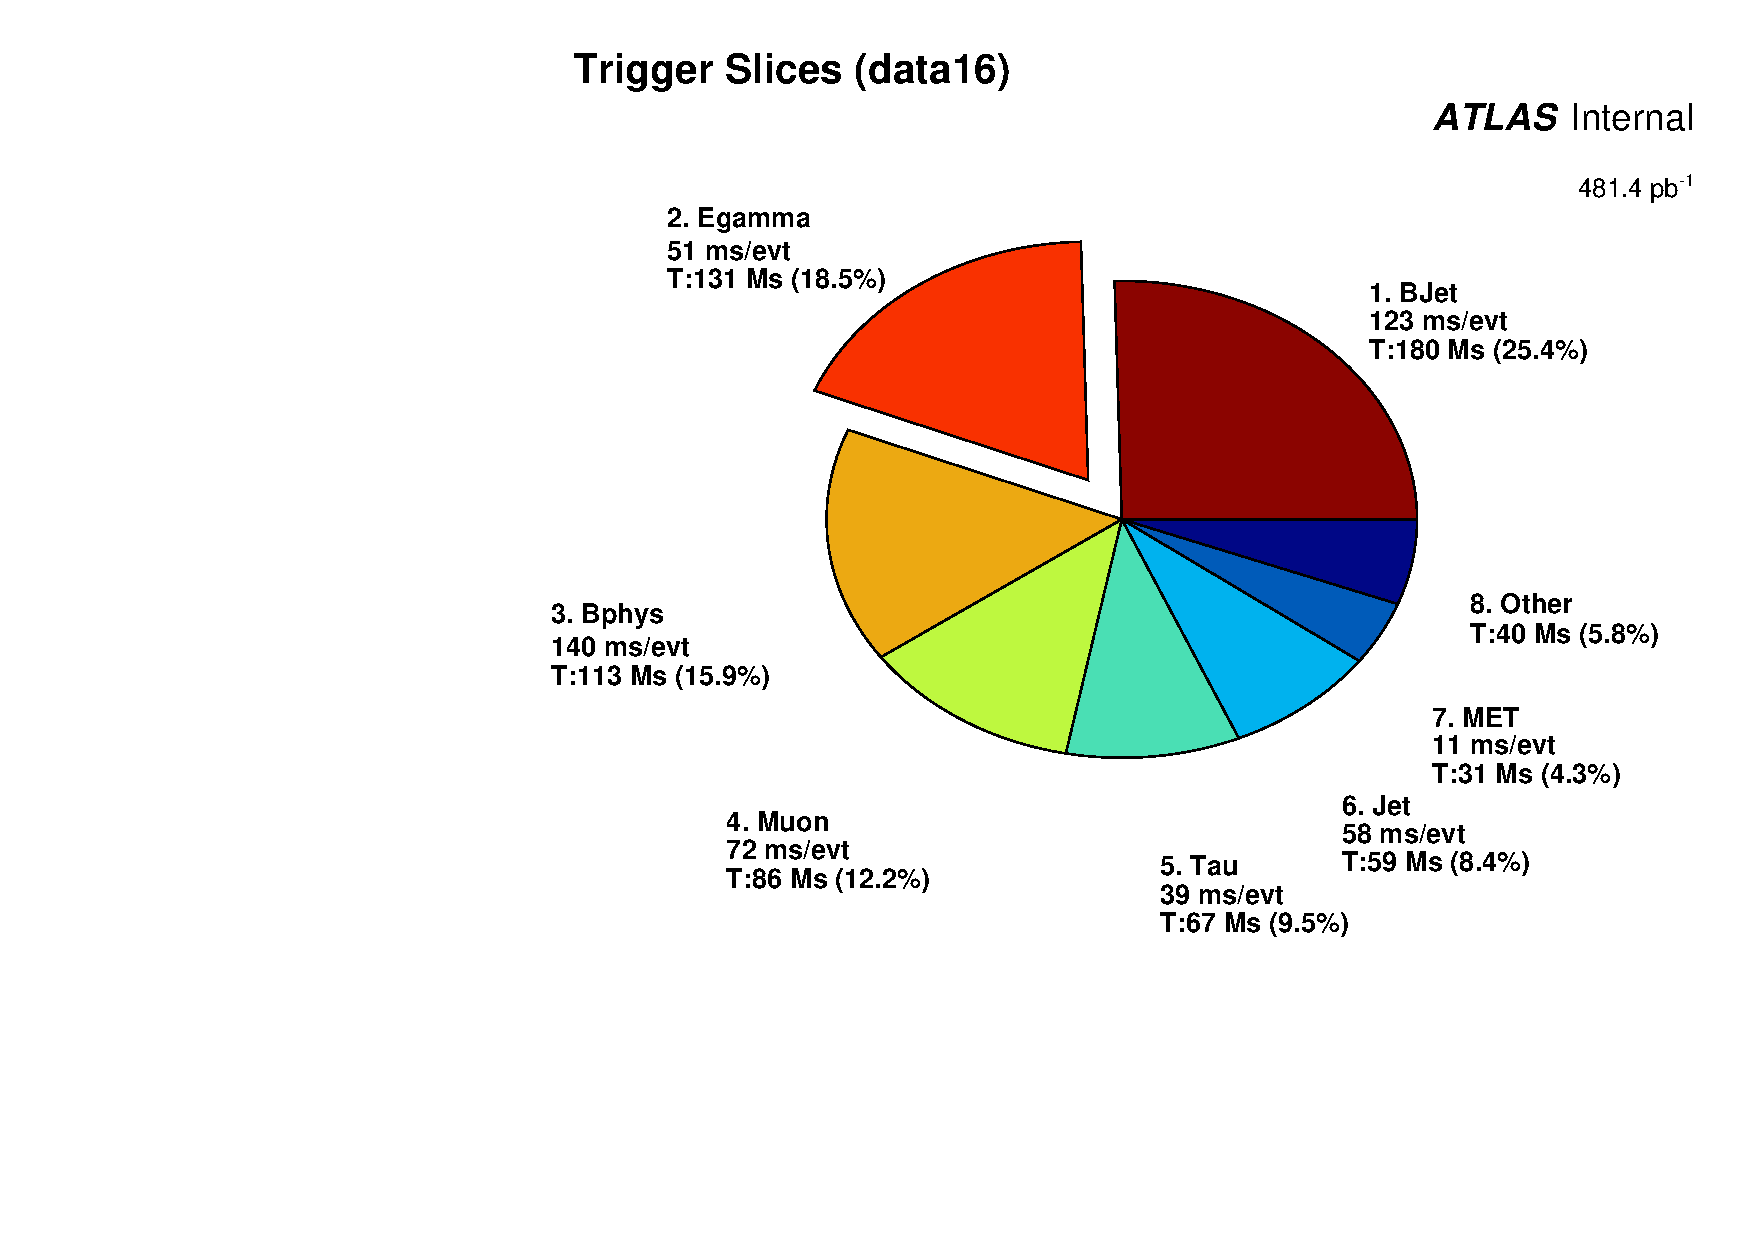
\includegraphics[width=\textwidth]{appendices/figures/menu_cpu_measurements/run2_slice_cpu_slices_pie_data16.pdf}
\caption{}%
\label{fig:run2_monitored_cpu_per_group_data16}
\end{subfigure}
\hfill
%\hspace{0.01\textwidth}
\begin{subfigure}[c]{.48\textwidth}
  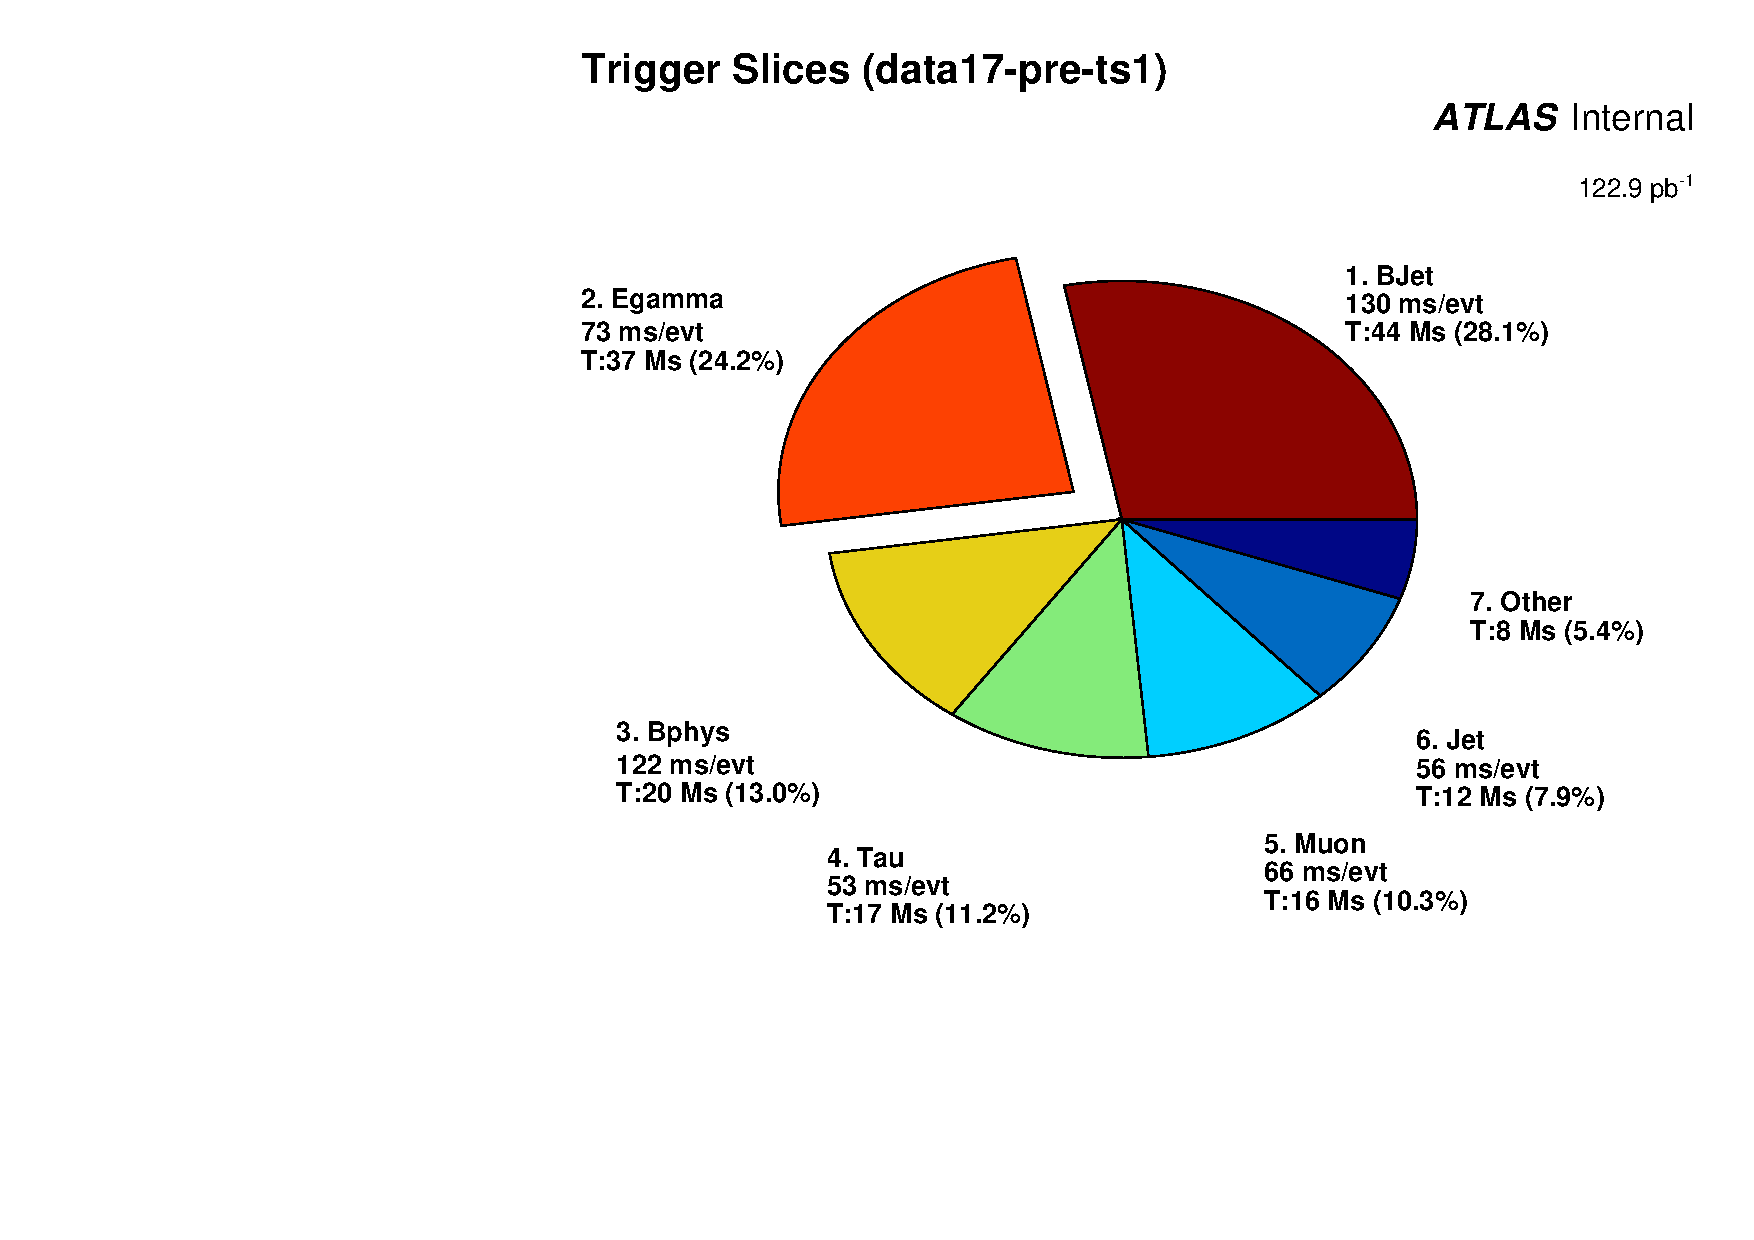
\includegraphics[width=\textwidth]{appendices/figures/menu_cpu_measurements/run2_slice_cpu_slices_pie_data17-pre-ts1.pdf}
\caption{}%
\label{fig:run2_monitored_cpu_per_group_data17_pre}
\end{subfigure} \\
\begin{subfigure}[c]{.48\textwidth}
  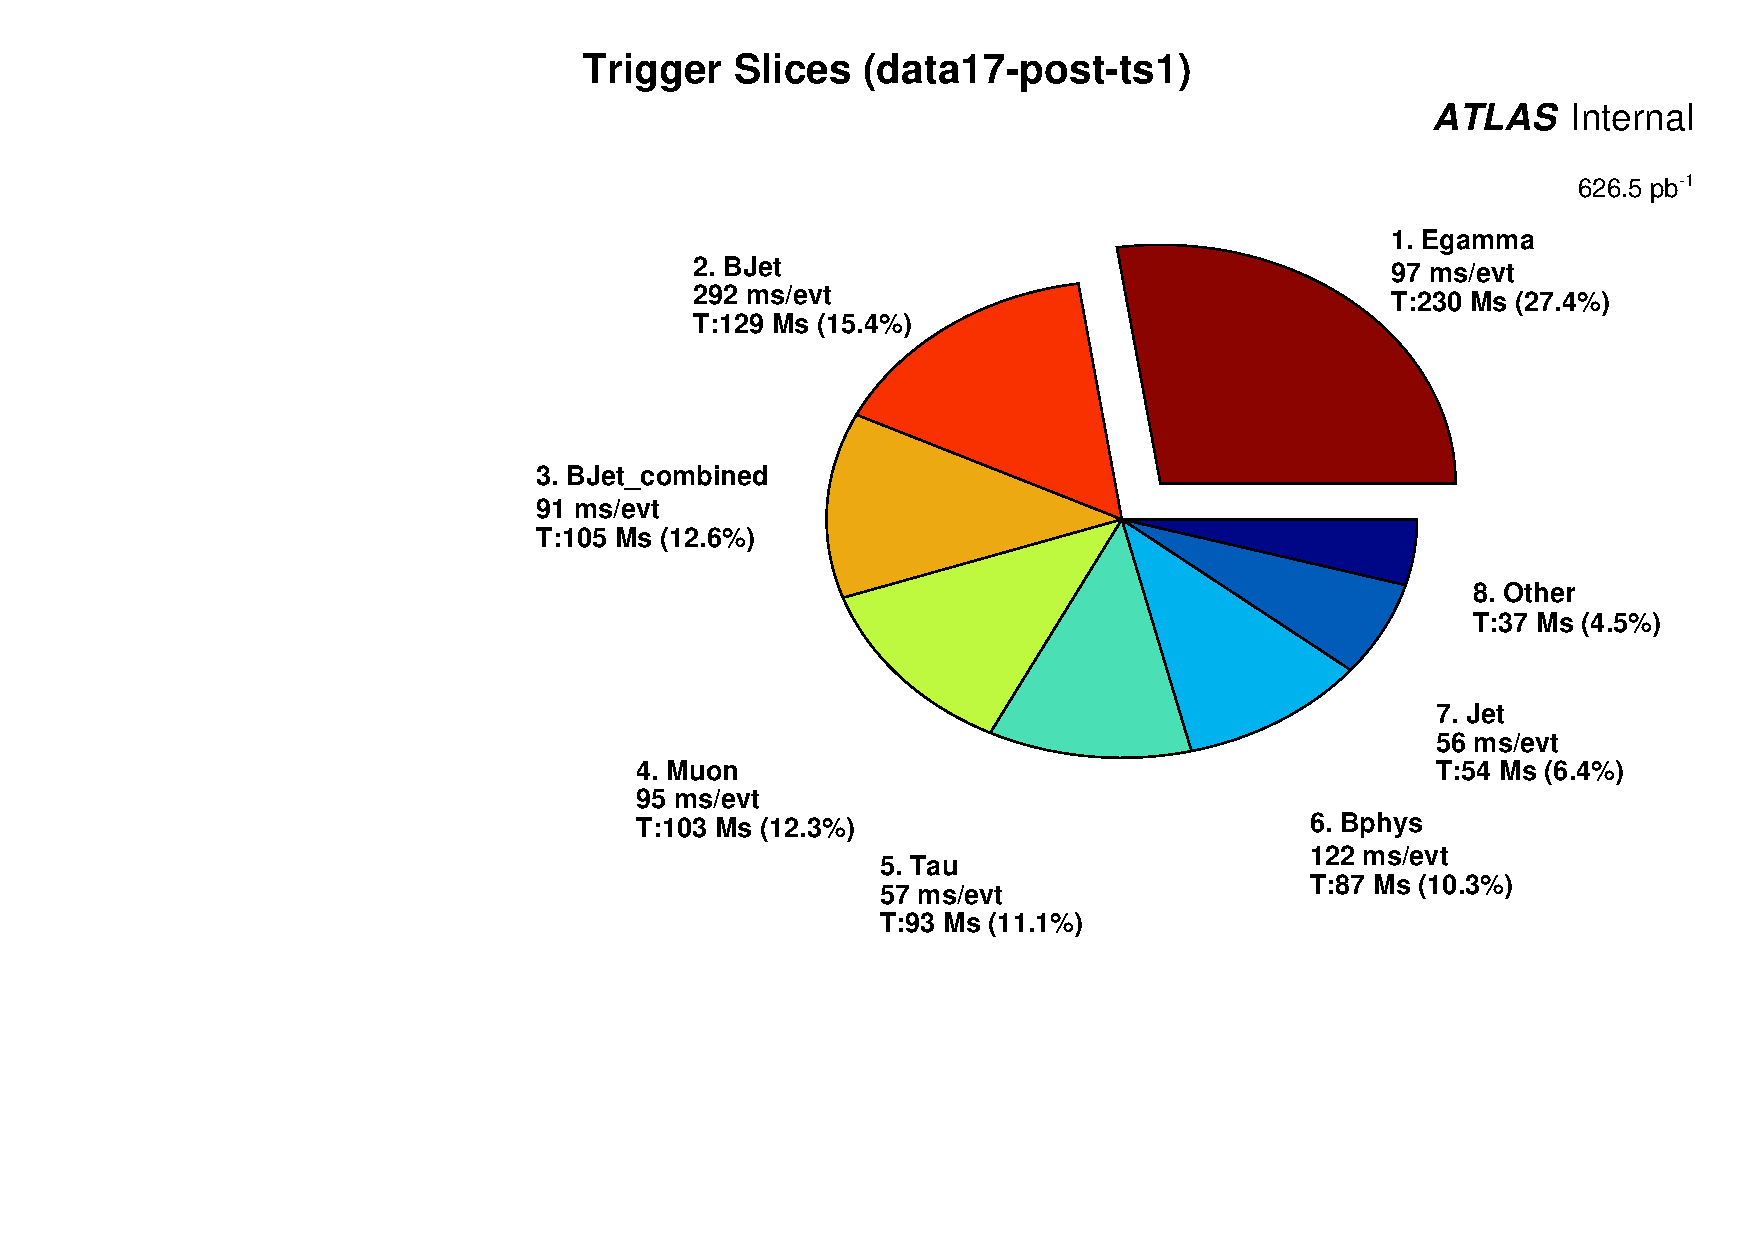
\includegraphics[width=\textwidth]{appendices/figures/menu_cpu_measurements/run2_slice_cpu_slices_pie_data17-post-ts1.pdf}
\caption{}%
\label{fig:run2_monitored_cpu_per_group_data17_post}
\end{subfigure} 
\begin{subfigure}[c]{.48\textwidth}
  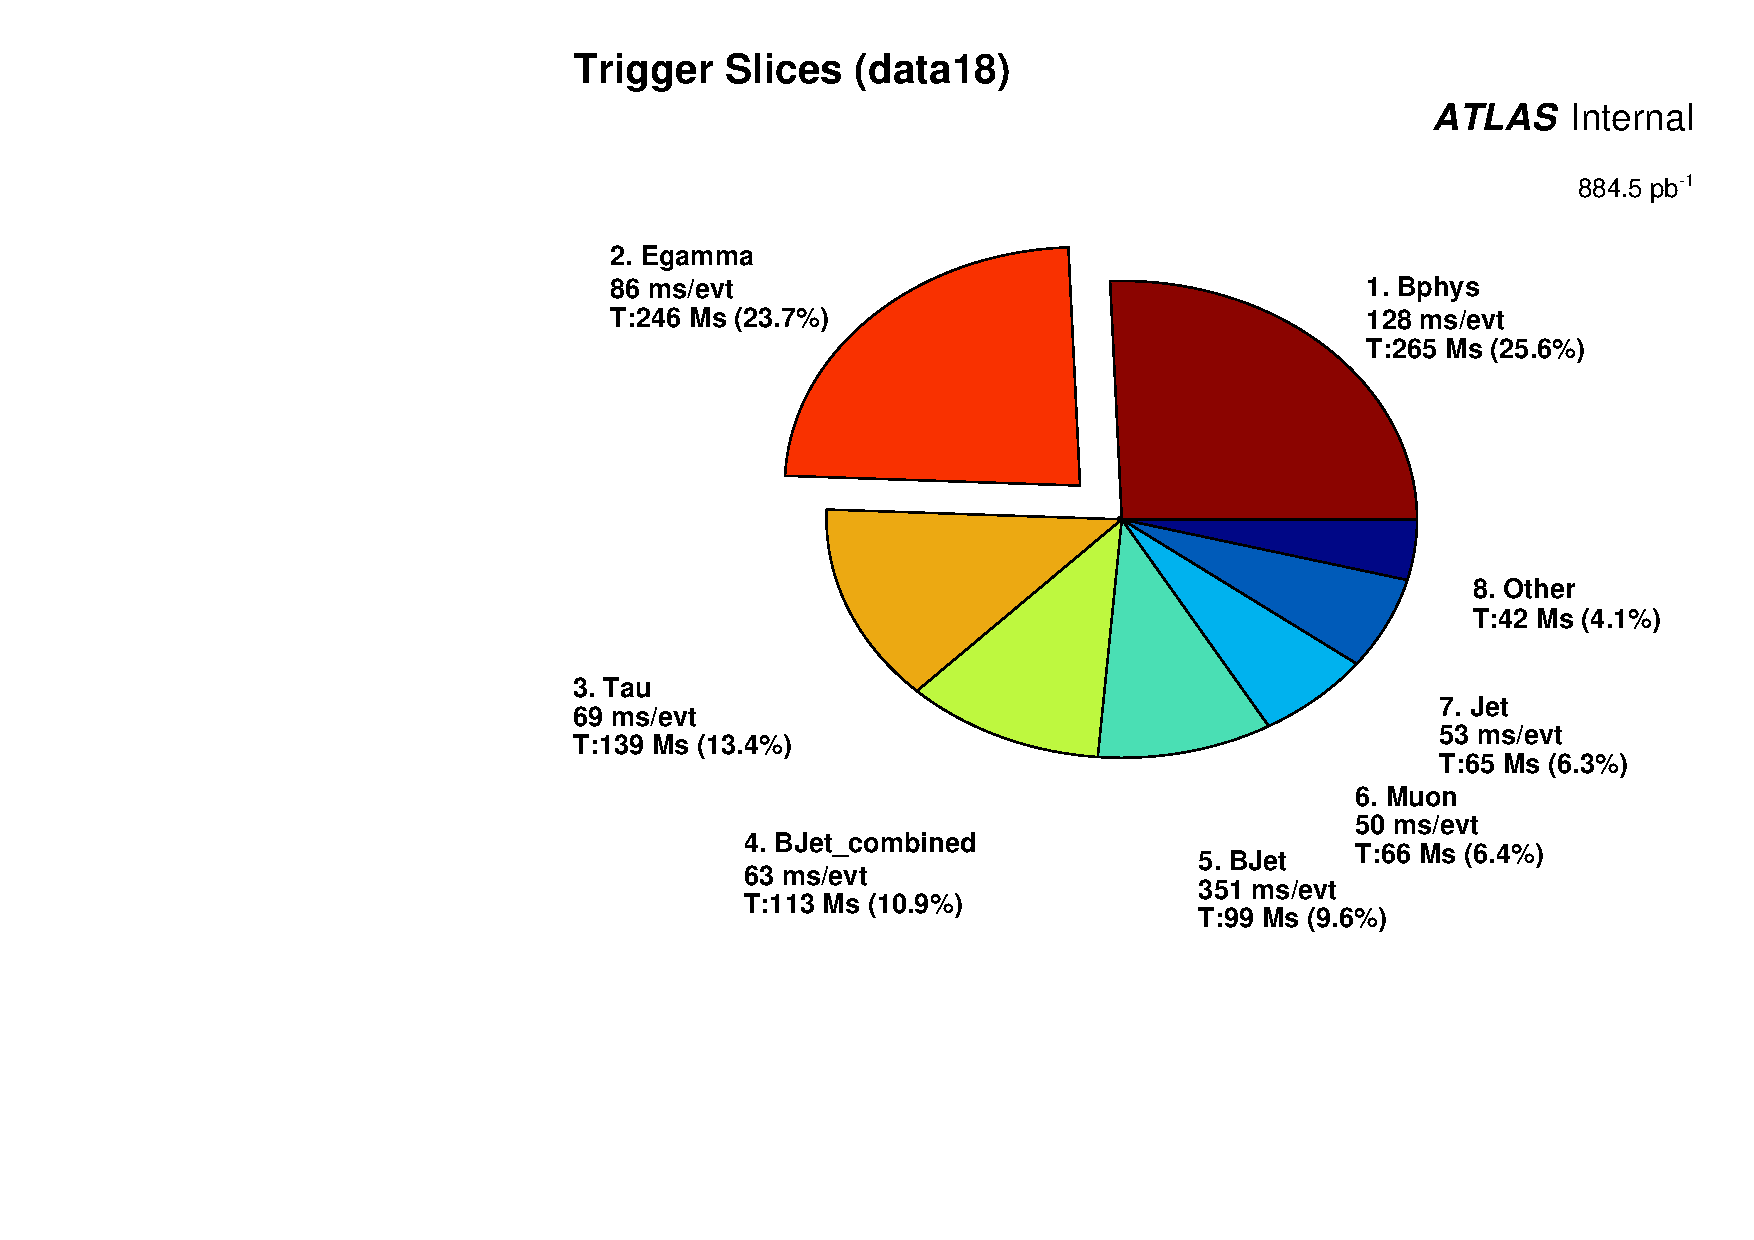
\includegraphics[width=\textwidth]{appendices/figures/menu_cpu_measurements/run2_slice_cpu_slices_pie_data18.pdf}
\caption{}%
\label{fig:run2_monitored_cpu_per_group_data18}
\end{subfigure} 
\caption{\label{fig:run2_monitored_cpu_per_group}CPU time demanded by each
  group. 2016 data are shown in (a), before 2017 TS1 in (b), after 2017 TS1 in
  (c) and 2018 in (d). The groups are in decreasing order based on the
  total CPU time demanded during the cost monitoring samplings. Emphasis is
  given in the graph to the \egamma{} group. Each group total time is displayed
  in the third line after for each group followed by the fraction of when
  considering the full HLT CPU time. The average CPU time per all HLT processed
  events is shown in the second line.
}
\end{figure}

\begin{figure}[h!tb]
\centering
\begin{subfigure}[c]{.48\textwidth}
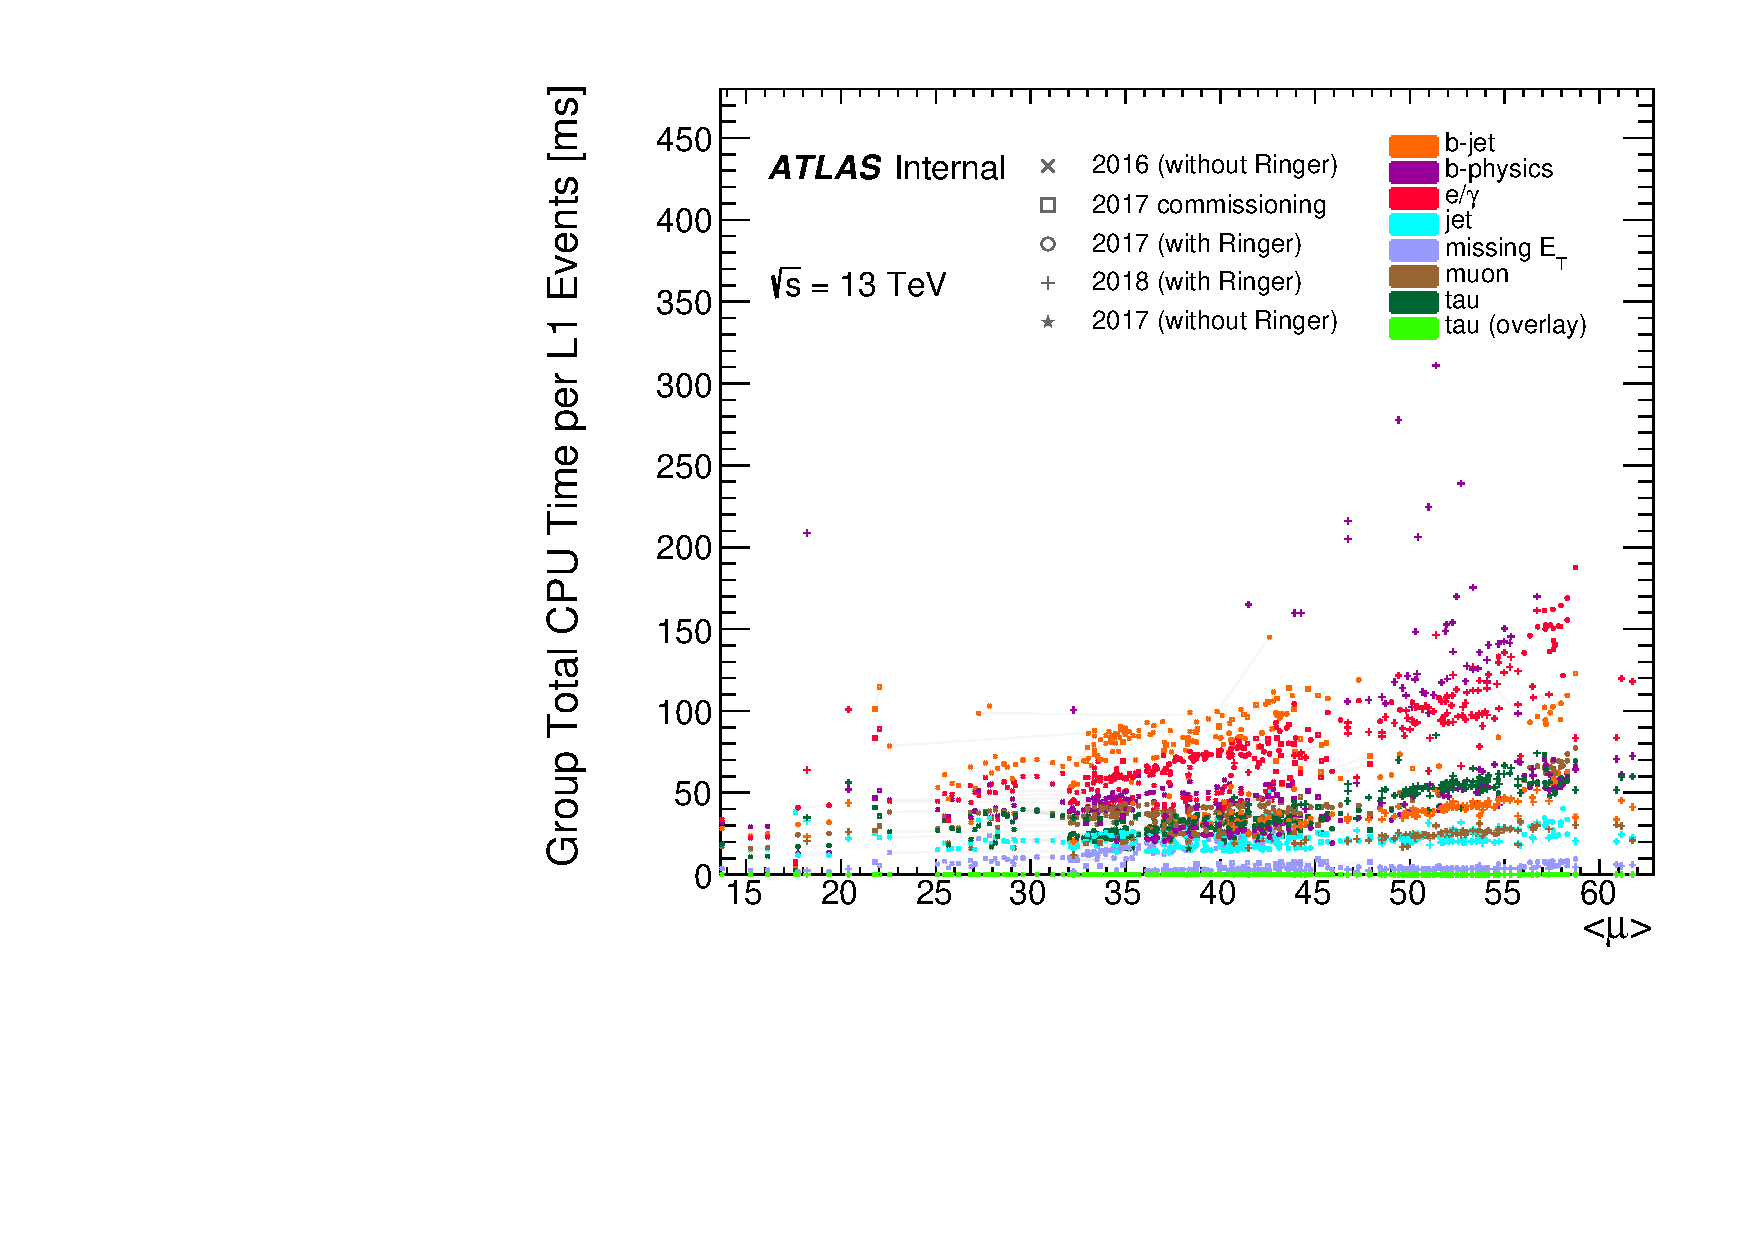
\includegraphics[width=\textwidth]{appendices/figures/menu_cpu_measurements/run2_slice_cpu_total_all_data.pdf}
\caption{}%
\label{fig:run2_monitored_cpu_per_mu_norm_l1_evt}
\end{subfigure}
\hfill
%\hspace{0.01\textwidth}
\begin{subfigure}[c]{.48\textwidth}
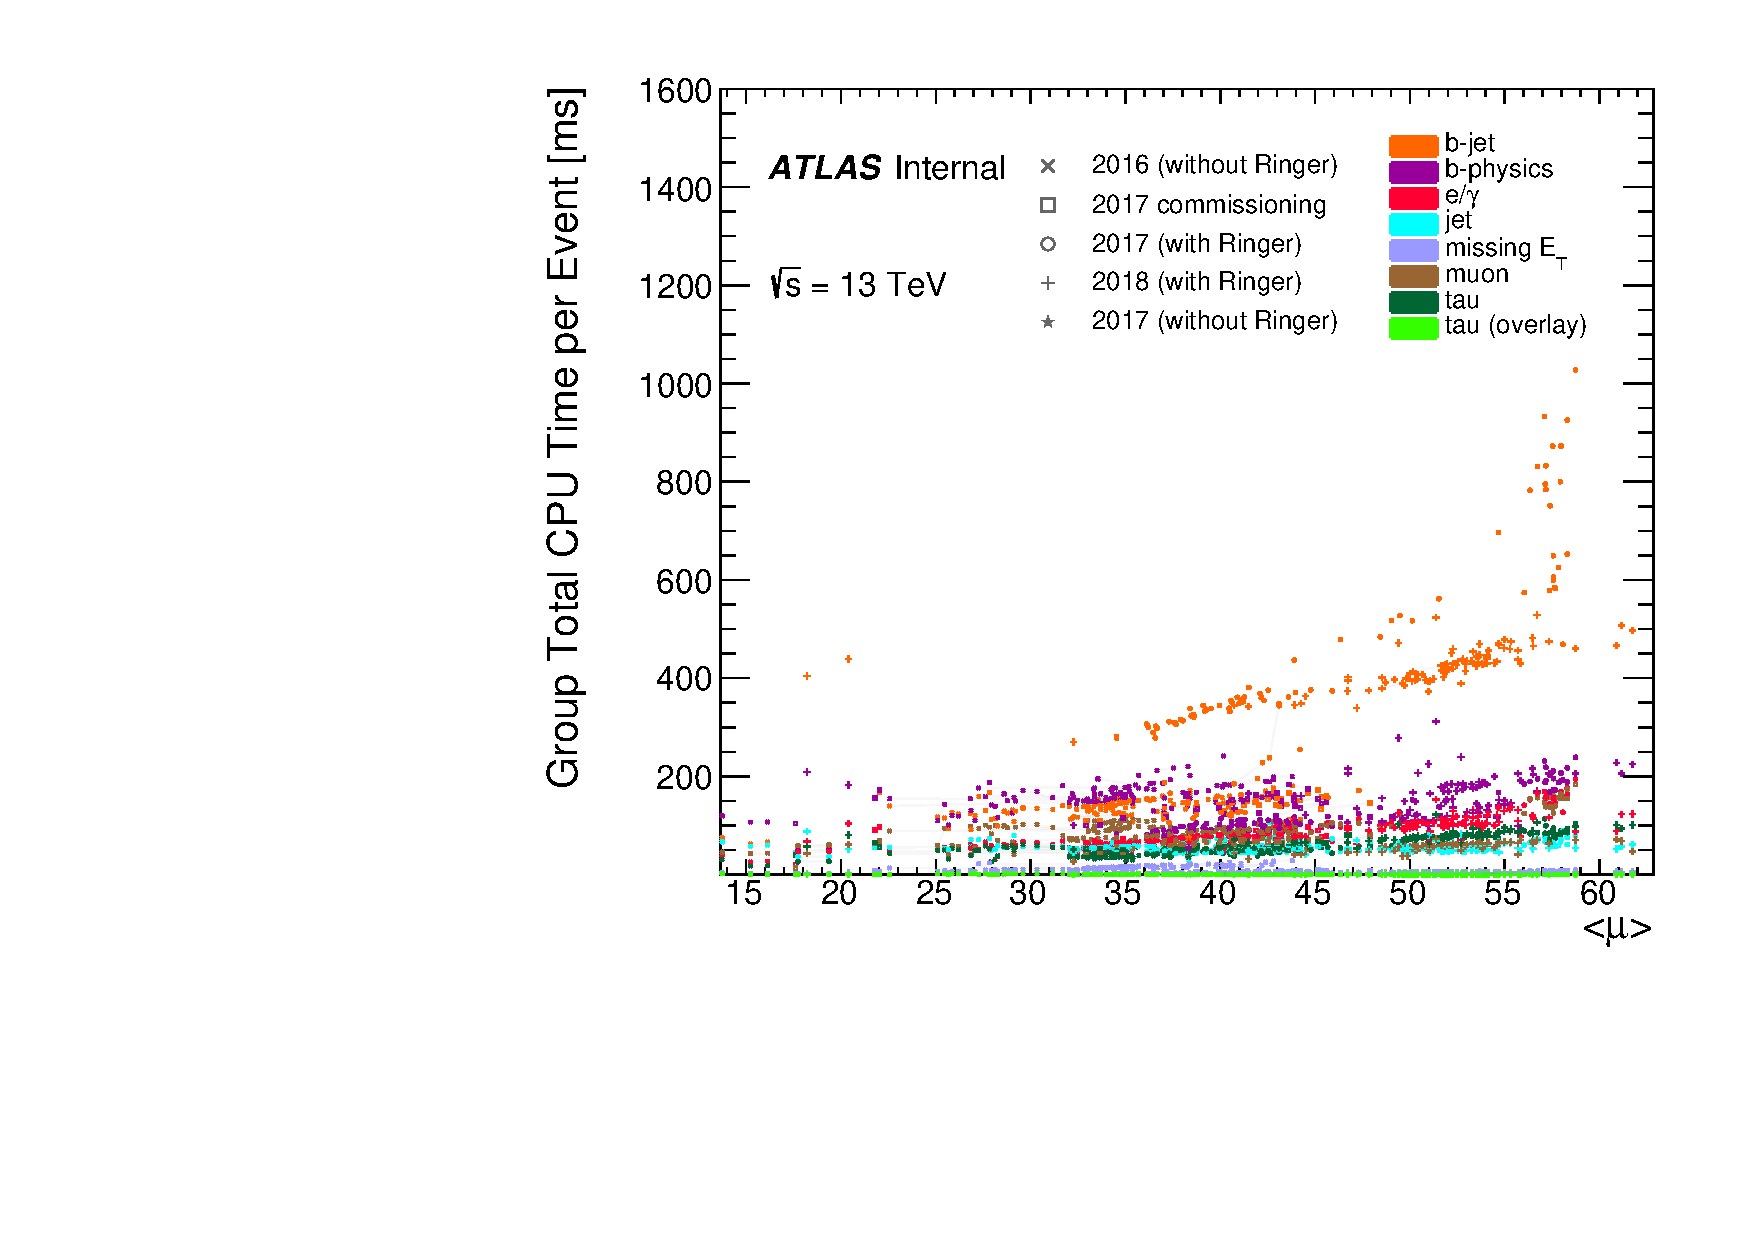
\includegraphics[width=\textwidth]{appendices/figures/menu_cpu_measurements/run2_slice_cpu_time_per_event_all_data.pdf}
\caption{}%
\label{fig:run2_monitored_cpu_per_mu_norm_group_evt}
\end{subfigure} \\
\caption{\label{fig:run2_monitored_cpu_per_mu}CPU time normalized by the
total number of L1 output (a) and each trigger signature events (b) as
function of \avgmu{}. The measurement colors are used to determine the signature
group and the marker style determine the period. 2016 data are shown with
crosses, before 2017 TS1 with squares, after 2017 TS1 with circles, 2018 with
plus marks and special data taking luminosity blocks during before 2017 TS1
configured without \rnn with stars. }
\end{figure}

Figure~\ref{fig:run2_monitored_egamma_cpu} shows the CPU demands according to
some trigger sub-groups within \egamma{}. Combined triggers refer to those that
require other physics object then the group they are placed in, i.e. an electron
trigger require a jet or a muon; as opposed to pure triggers. Additional
splitting is applied to electrons triggers depending on the energy of the
electron legs: a group for when all are above \SI{15}{\GeV} (affected by \rnn
operation after 2017 TS1); another for the case where all are below
\SI{15}{\GeV} (not affected); and a last group containing energy-thresholds at
both groups (partially affected by the \rnn).

\begin{figure}[h!tb]
\centering
\begin{subfigure}[c]{.48\textwidth}
  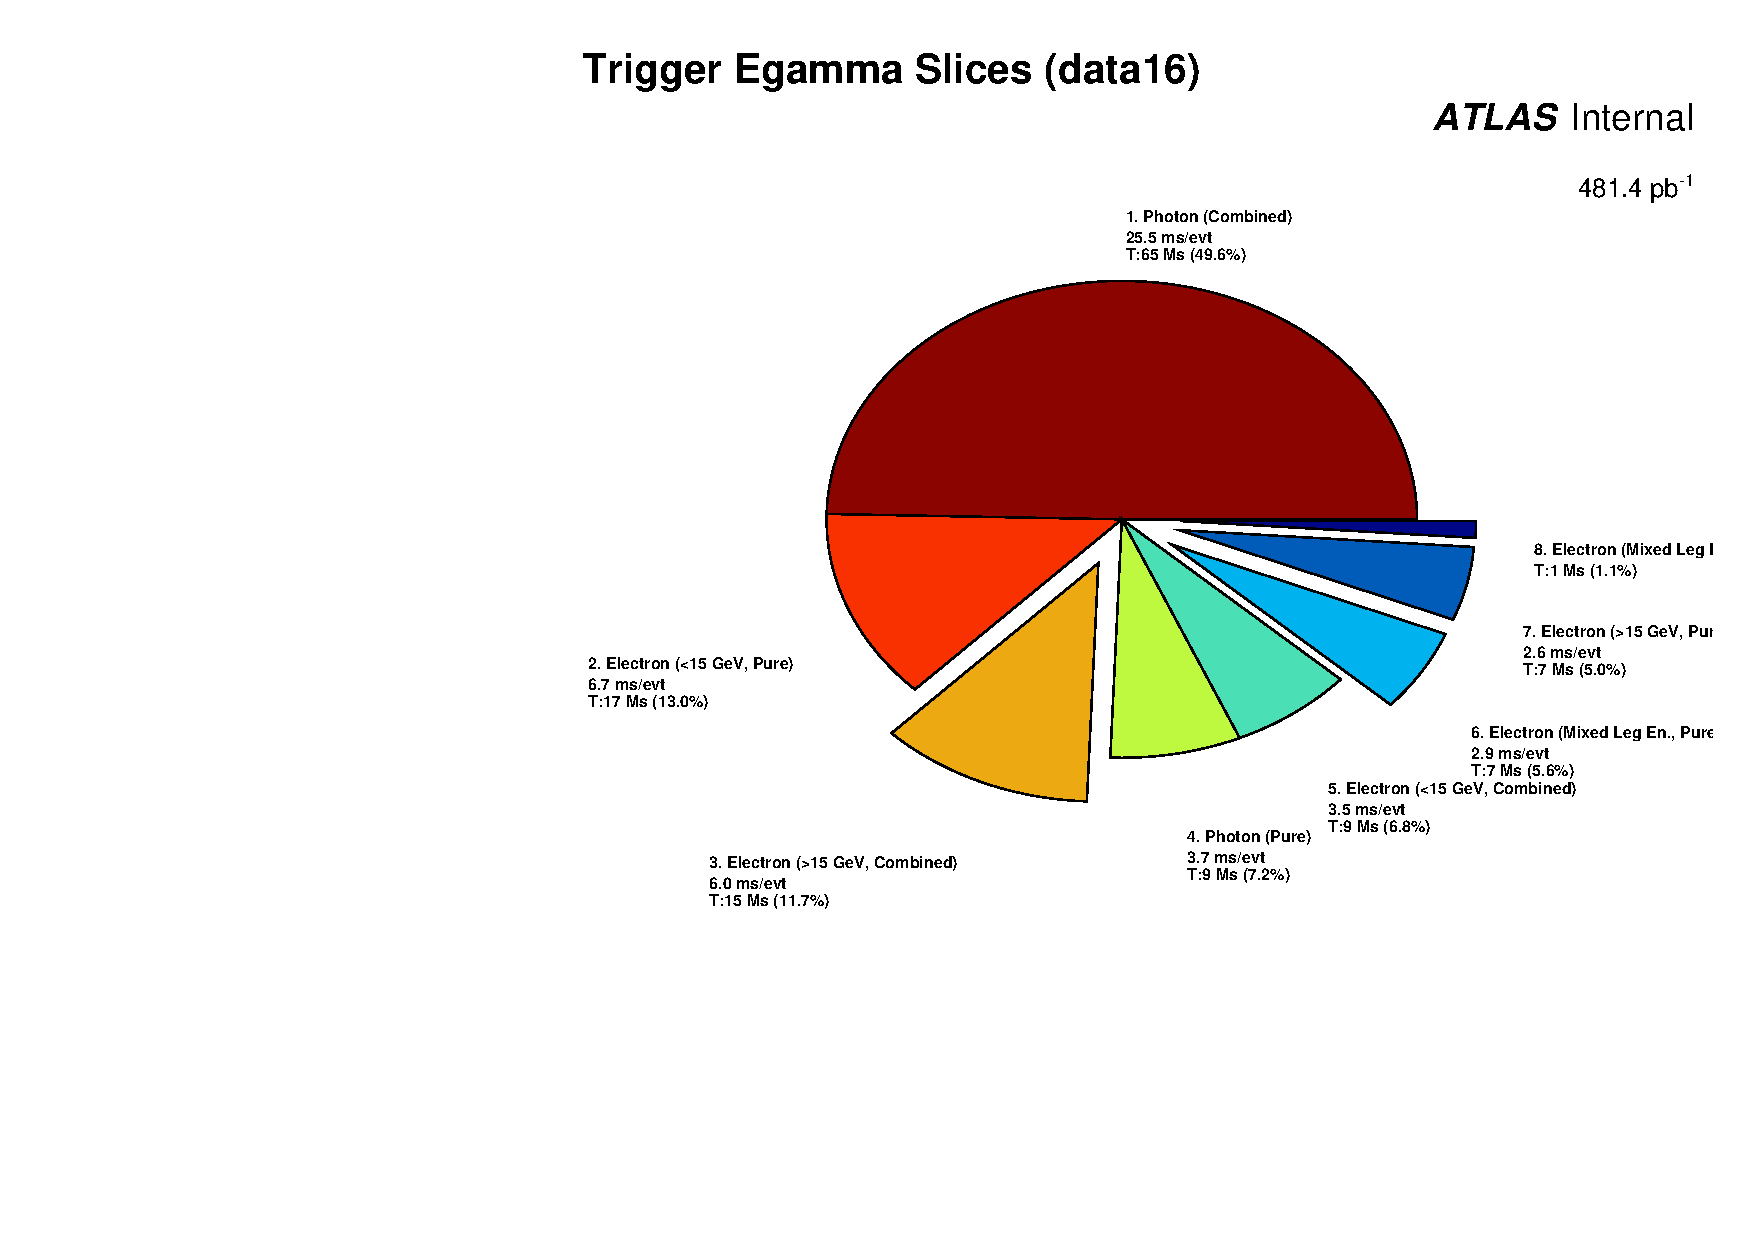
\includegraphics[width=\textwidth]{appendices/figures/menu_cpu_measurements/run2_slice_cpu_egamma_pie_data16.pdf}
\caption{}%
\label{fig:run2_monitored_egamma_cpu_data16}
\end{subfigure}
\hfill
%\hspace{0.01\textwidth}
\begin{subfigure}[c]{.48\textwidth}
  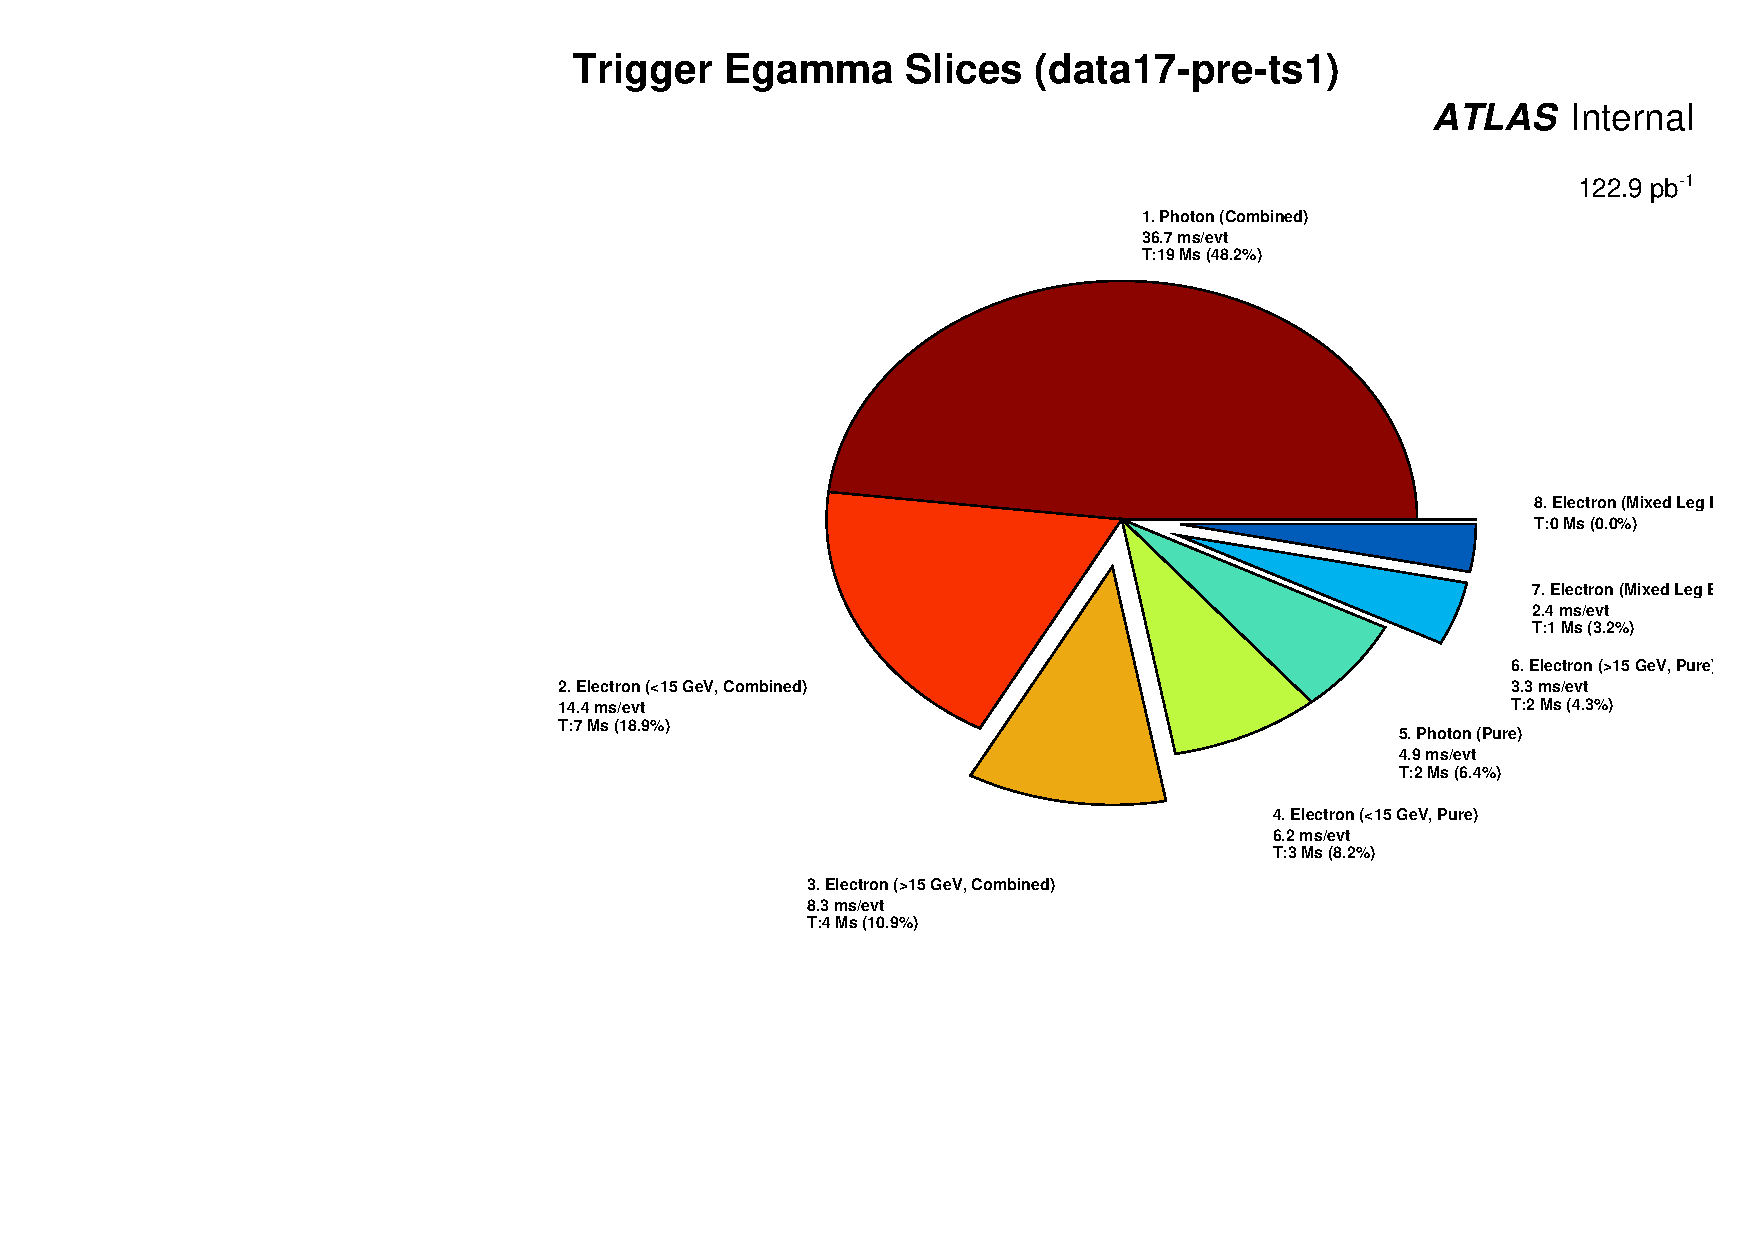
\includegraphics[width=\textwidth]{appendices/figures/menu_cpu_measurements/run2_slice_cpu_egamma_pie_data17-pre-ts1.pdf}
\caption{}%
\label{fig:run2_monitored_egamma_cpu_data17_pre}
\end{subfigure} \\
\begin{subfigure}[c]{.48\textwidth}
  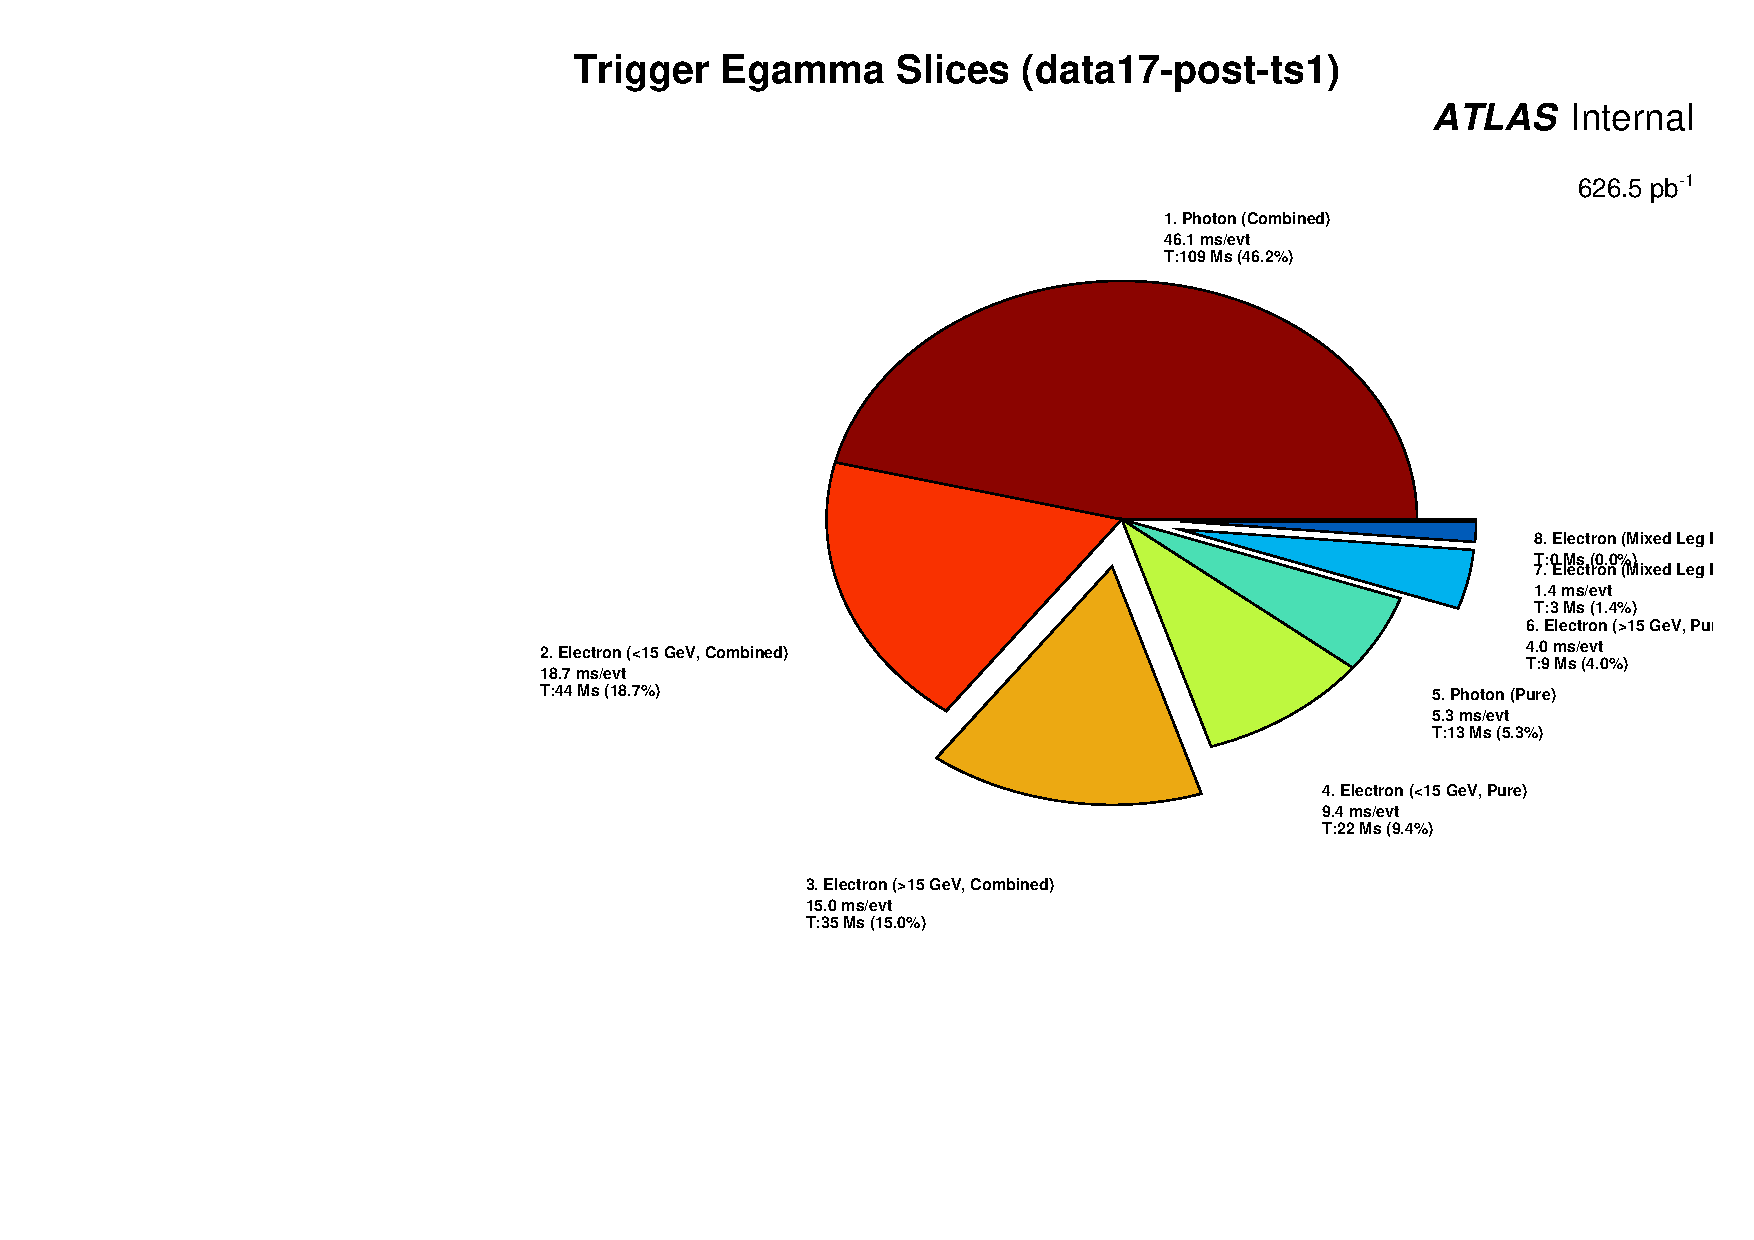
\includegraphics[width=\textwidth]{appendices/figures/menu_cpu_measurements/run2_slice_cpu_egamma_pie_data17-post-ts1.pdf}
\caption{}%
\label{fig:run2_monitored_egamma_cpu_data17_post}
\end{subfigure}
\begin{subfigure}[c]{.48\textwidth}
  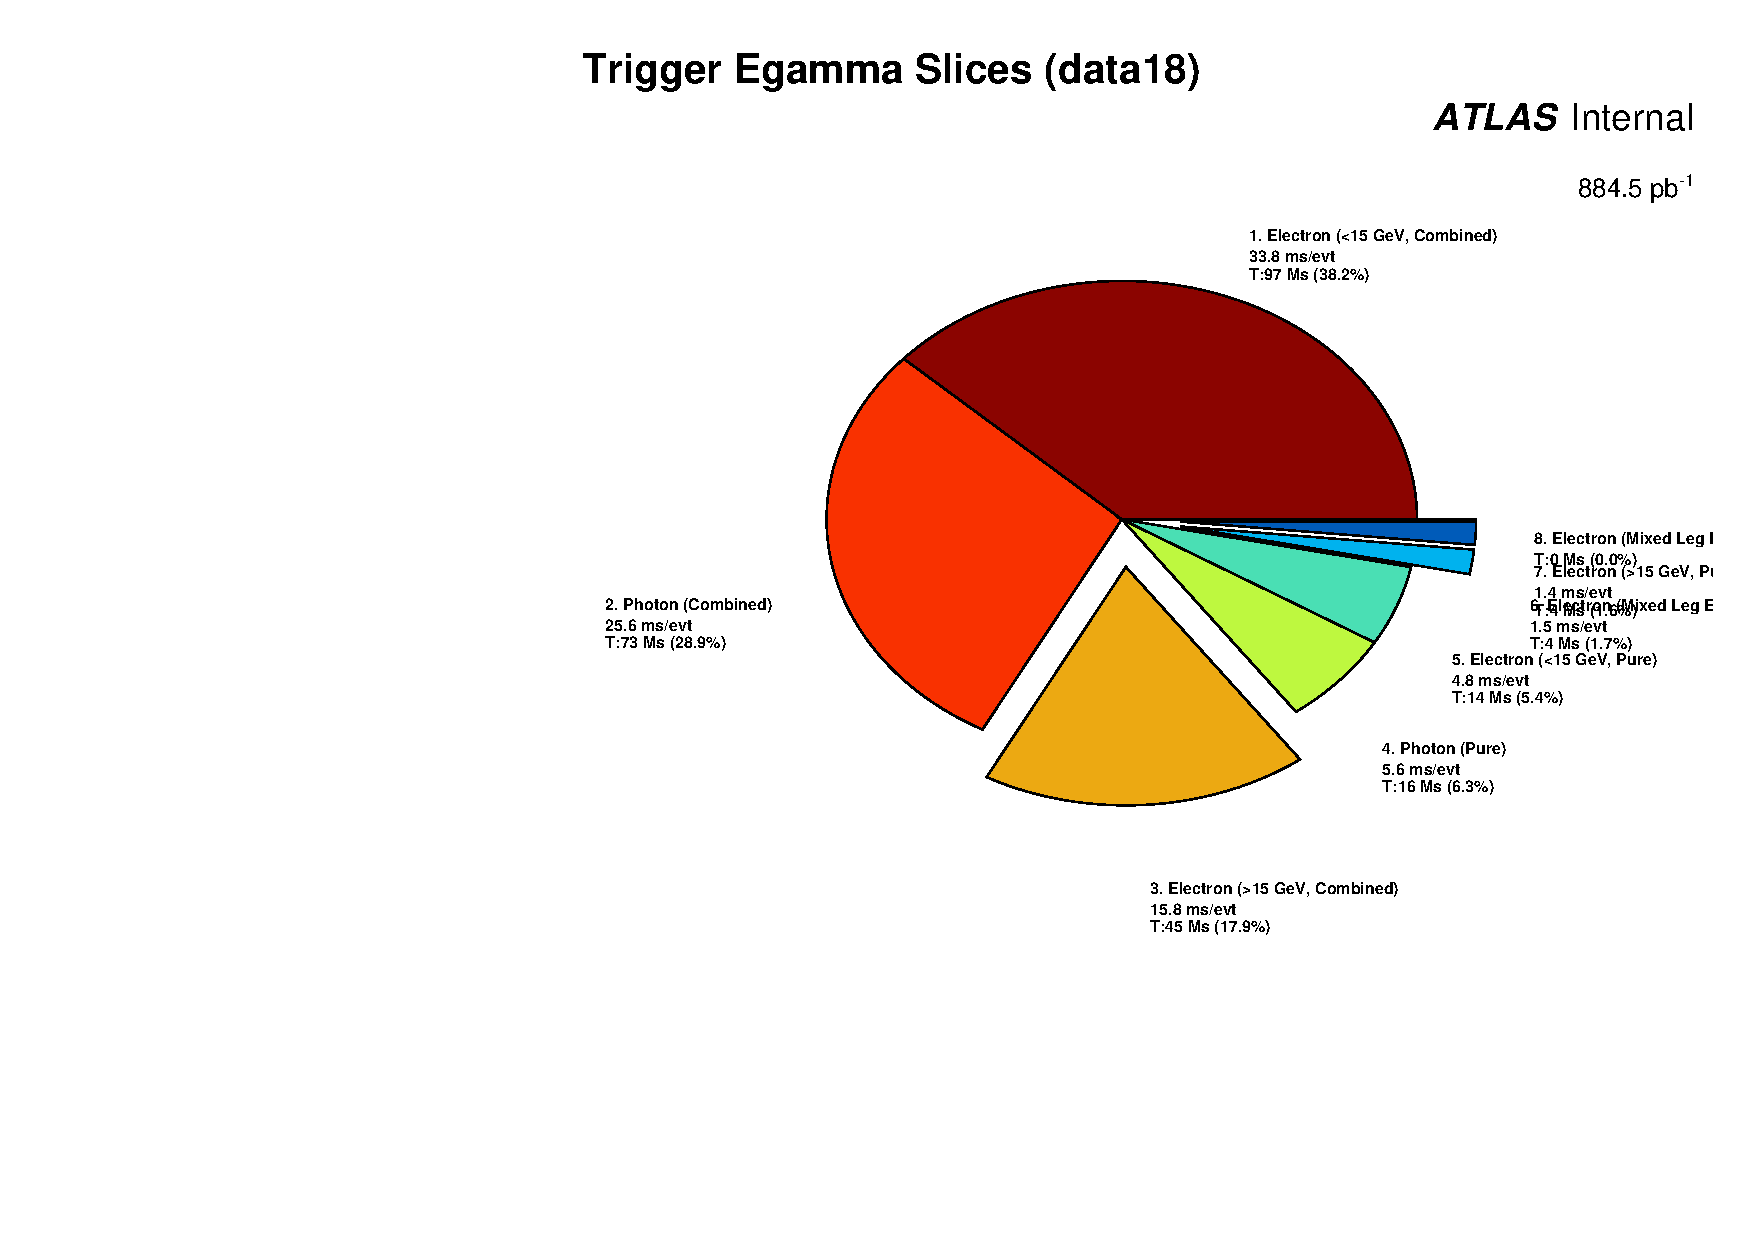
\includegraphics[width=\textwidth]{appendices/figures/menu_cpu_measurements/run2_slice_cpu_egamma_pie_data18.pdf}
\caption{}%
\label{fig:run2_monitored_egamma_cpu_data18}
\end{subfigure}
\caption{\label{fig:run2_monitored_egamma_cpu}CPU time demanded by
\egamma{} triggers grouped by the leg configurations. The groups are in
decreasing order based on the total CPU time demanded during the cost monitoring
samplings. The groups where \rnn changed the configuration during Run~2 are
dislocated with respect to the center. Emphasis is given in the graph to the
groups where \rnn{} changed the configuration during Run~2. Each group total
time is displayed in the third line after for each group followed by the
fraction of when considering the full HLT CPU time. The average CPU time per all
HLT processed events is shown in the second line.
}
\end{figure}

The most demanding \egamma{} sub-groups are combined photon triggers and
combined electron triggers with legs below \SI{15}{\GeV}. Together, they demand
around $2/3$ of the \egamma{} group CPU. When considering pure photon triggers
and combined electron triggers to take all groups unaffected by the \rnn
operation during Run~2, fraction goes to nearly $3/4$ of the \egamma{} CPU.\@
Hence, there is a great potential for the \rnn{} to further release resources in
next data-takings by enabling its operation for these other groups, namely
triggers with electron legs below \SI{15}{\GeV} and photon combined triggers.

To have an idea of the fraction of P1 CPU that could benefit of a
more efficient early selection as offered by the \rnn{}, we show the most CPU
demanding triggers containing at least an electron or a photon in
Table~\ref{tab:top_cpu_electrons} and Table~\ref{tab:top_cpu_photons},
respectively. It can be observed that these triggers alone required about
\SI{15}{\%} to \SI{30}{\%} of the total CPU during Run~2. Except for a few
triggers that do not apply any requirement in the electron or photon legs
(i.e.\@ the g0 and etcut triggers), the \rnn{} may be able to bring considerable
additional impact if set to operate on the electron and photon legs.

%As shown in Section~\ref{top:menu_cpu}, a great potential for saving CPU is
%available if the \rnn{} is developed for selecting electrons with
%$\et<\SI{15}{\GeV}$. Additionally, as many of those triggers are prescaled to
%reduce their output rate in addition to the CPU limitations, it is possible that
%the \rnn{} algorithm can allow to reduce the pre-scale factor if it is capable
%of impacting the \hlt{} fake rate as it was the case of the factor of
%\SI{2}{$\times$} reduction for the duplicated trigger during 2017
%(Section~\ref{ssec:2017_ringer_operation}).

\FloatBarrier

\begin{table}[!ht]
    \centering
    \caption{\label{tab:top_cpu_electrons}Most-demanding electron triggers using
    Run 2 cost-monitoring data. The triggers are sorted out in decreasing order
    using the integrated CPU time (in seconds), while the CPU demands are shown in
    percentage when considering the total P1 CPU processing time in cost
    monitorings. Before TS1 data are labelled as {data17-}, whereas {data17+}
    dedicates to the remaining 2017 runs.}
    \resizebox{\textwidth}{!}{%
      \begin{tabular}{p{20cm}cccc}
    \hline\hline
    Trigger with at least one electron leg & \multicolumn{4}{c}{P1 Total Trigger Time [\%]} \\
    \hline
    data type&
    data16 &
    data17-&
    data17+&
    data18 \\
    \hline
    HLT\_e60\_etcut\_trkcut\_L1EM24VHIM\_xs30\_j15\_perf\_xe30\_6dphi15\_mt35&
    &
    &
    2.48&
    2.81 \\
    HLT\_e7\_lhmedium\_nod0\_mu24&
    0.82&
    1.31&
    1.62&
    1.98 \\
    HLT\_e9\_lhvloose\_nod0\_mu20\_mu8noL1\_L1EM7\_MU20&
    &
    &
    &
    2.19 \\
    HLT\_mu20\_mu8noL1\_e9\_lhvloose\_nod0&
    &
    1.19&
    1.27&
    1.76\\
    HLT\_e5\_lhmedium\_nod0\_j40\_xe80\_pufit\_2dphi10\_L1XE60&
    &
    1.79&
    &
    \\
    HLT\_mu20\_mu8noL1\_e9\_lhvloose\_nod0\_L1EM7\_MU20&
    &
    1.95&
    2.01&
    2.65\\
    HLT\_e5\_lhloose\_nod0\_j40\_xe70\_pufit\_2dphi10\_L1XE60&
    &
    0.25&
    1.28&
    1.08 \\
    HLT\_e9\_lhvloose\_nod0\_mu20\_mu8noL1&
    &
    &
    &
    1.35 \\
    HLT\_e5\_lhmedium\_nod0\_j50\_xe80\_\_2dphi10\_L1J40\_XE50\_DPHI-J20s2XE50pufit&
    &
    0.51&
    0.69&
    0.82 \\
    HLT\_e5\_lhtight\_nod0\_e14\_etcut\_Jpsiee\_L1JPSI-1M5-EM12&
    &
    &
    2.44&
    1.53 \\
    HLT\_e28\_lhtight\_nod0\_noringer\_ivarloose\_L1EM24VHIM&
    &
    &
    0.56&
    \\
    HLT\_e5\_lhloose\_nod0\_mu4\_j30\_xe40\_pufit\_2dphi10\_L1MU4\_J30\_XE40\_DPHI-J20s2XE30&
    &
    0.34&
    0.50&
    0.55 \\
    HLT\_e28\_lhtight\_nod0\_L1EM24VHIM\_e15\_etcut\_L1EM7\_Zee&
    &
    0.59&
    0.28&
    0.30 \\
    HLT\_e26\_lhmedium\_nod0\_mu8noL1&
    &
    0.18&
    0.11&
    0.47 \\
    HLT\_e5\_lhtight\_nod0\_e14\_etcut\_Jpsiee&
    &
    0.91&
    2.3&
     \\
    HLT\_e5\_lhtight\_nod0 (rerun)&
    0.28&
    0.39&
    0.36&
    0.40 \\
    HLT\_e26\_lhtight\_nod0\_e15\_etcut\_L1EM7\_Zee&
    0.53&
    0.02&
    0.02&
    0.07 \\
    HLT\_2e5\_lhmedium\_nod0\_j70\_j50\_0eta490\_invm900j50\_L1MJJ-700&
    &
    &
    &
    0.64 \\
    HLT\_e26\_lhmedium\_nod0\_L1EM22VHIM\_mu8noL1&
    &
    0.42&
    0.34&
    \\
    HLT\_e13\_etcut\_trkcut\_L1EM12&
    0.44&
    0.30&
    &
    \\
    HLT\_e28\_lhmedium\_nod0\_L1EM24VHIM\_mu8noL1&
    &
    0.04&
    0.02&
    0.02 \\
    HLT\_2e5\_lhmedium\_nod0\_j70\_j50\_0eta490\_invm900j50\_L1MJJ-500-NFF &
    &
    &
    &
    0.52 \\
    HLT\_e5\_lhtight\_nod0\_e9\_etcut\_Jpsiee\_L1JPSI-1M5-EM7 &
    &
    &
    0.94&
    0.56 \\
    HLT\_e14\_etcut\_e5\_lhtight\_nod0\_Jpsiee &0.67& & & \\
    HLT\_e13\_etcut\_trkcut\_xs30\_j15\_perf\_xe30\_6dphi15\_mt35 &
    0.14& 0.29& 0.34& 0.29 \\
    \hline
    Total& 2.89 & 10.47 & 17.64 & 20.10\\
    \hline
    \hline
    \end{tabular}
    }
    \end{table}
    
\begin{table}[!ht]
    \centering
    \caption{\label{tab:top_cpu_photons}Most-demanding photon triggers using
    Run 2 cost-monitoring data. Trigger and CPU information as in
    Table~\ref{tab:top_cpu_electrons}.}
    \resizebox{\textwidth}{!}{%
      \begin{tabular}{p{20cm}cccc}
    \hline\hline
    Trigger with at least one photon leg & \multicolumn{4}{c}{P1 Total Trigger Time [\%]} \\
    \hline
    data type&
    data16 &
    data17-&
    data17+&
    data18 \\
    \hline
    HLT\_g27\_medium\_L1EM24VHI\_2j15\_gsc35\_bmv2c1077\_split\_2j35\_0eta490&
    4.21&
    4.81&
    \\
    HLT\_g35\_loose\_L1EM24VHI\_mu15noL1\_mu2noL1&
    3.02&
    &
    &
    \\
    HLT\_g27\_medium\_L1EM24VHI\_2j35\_bmv2c1077\_split\_2j35\_0eta490&
    &
    &
    0.00&
    1.47\\
    HLT\_g40\_tight\_icalotight\_L1EM24VHI\_mu15noL1\_mu2noL1&
    &
    1.19&
    1.08&
    1.13\\
    HLT\_g20\_loose\_L1EM15I\_mu4\_iloose\_taumass&
    2.69&
    &
    &
    \\
    HLT\_g25\_medium\_L1EM24VHI\_tau25\_dikaonmasstight\_tracktwo\_60mVis10000&
    2.36&
    &
    &
    \\
    HLT\_g25\_medium\_L1EM24VHI\_tau25\_kaonpi2\_tracktwo\_50mVis10000&
    &
    0.95&
    0.61&
    0.60\\
    HLT\_g0\_hiptrt\_L1EM24VHIM&
    &
    0.84&
    0.80&
    0.74\\
    HLT\_g35\_tight\_icalotight\_L1EM24VHI\_mu15noL1\_mu2noL1&
    &
    0.70&
    0.63&
    0.65\\
    HLT\_g0\_hiptrt\_L1EM22VHI&
    0.81&
    0.29&
    0.28&
    0.26\\
    HLT\_g35\_medium\_L1EM24VHI\_tau25\_dipion3\_tracktwo\_60mVis10000&
    &
    &
    0.50&
    0.60\\
    HLT\_g10\_loose\_L1EM8I\_mu10\_iloose\_taumass&
    1.30&
    0.86&
    0.74&
    \\
    HLT\_g35\_loose\_L1EM24VHI\_mu18noL1&
    0.74&
    &
    &
    \\
    HLT\_g100\_tight\_L1EM24VHI\_3j50noL1&
    &
    0.29&
    0.29&
    0.48\\
    HLT\_g20\_loose\_L1EM15\_mu4\_iloose\_taumass&
    &
    1.17&
    1.58&
    \\
    HLT\_g35\_medium\_L1EM24VHI\_tau25\_singlepiontight\_tracktwo\_L1TAU12&
    0.48&
    &
    &
    \\
    HLT\_tau25\_mediumRNN\_tracktwoMVA\_tau20\_mediumRNN\_tracktwoMVA\_j70\_j50\_0eta490\_invm900j50\_L1MJJ-500-NFF&
    &
    &
    &
    0.35\\
    HLT\_g25\_medium\_tau25\_dikaonmasstight\_tracktwo\_60mVis10000&
    0.49&
    &
    &
    \\
    HLT\_g20\_loose\_mu4\_iloose\_taumass\_L1LFV-EM15I&
    0.68&
    0.27&
    0.29&
    0.24\\
    HLT\_g100\_tight\_L1EM22VHI\_3j50noL1&
    &
    0.10&
    0.10&
    0.16\\
    HLT\_tau25\_mediumRNN\_tracktwoMVA\_tau20\_mediumRNN\_tracktwoMVA\_j70\_j50\_0eta490\_invm900j50\_L1MJJ-700&
    &
    &
    &
    0.26\\
    HLT\_g35\_medium\_L1EM24VHI\_tau25\_dipion3\_tracktwoMVA\_60mVis10000&
    &
    &
    0.23\\
    HLT\_g25\_medium\_L1EM24VHI\_tau25\_singlepion\_tracktwoMVA\_50mVis10000&
    &
    &
    0.23\\
    \hline
    Total&
    12.58&
    10.87&
    11.73&
    7.38\\
    \hline
    \hline
    \end{tabular}
    }
    \end{table}
    


%\section{Supplementary Studies}\label{sec:supplementary_studies}

In this section, we bring the following supplementary preliminary evaluations
and open topics concerning the \rnn{}: the development of \rnn{} for the
selection of electrons with $\et<\SI{15}{\GeV}$ (Section~\ref{ssec:low_et}), the
selector efficiency when only \ecal{} information is employed
(Section~\ref{ssec:ecal_rnn}), some lumiblocks with possible inconsistent
trigger efficiencies (Section~\ref{ssec:lbs_lower_eff}) and additional
evaluations concerning the agreement analysis
(Section~\ref{ssec:supplementary_agreement}).

\subsection{\rnn{} for Triggering on Electrons Below \SI{15}{\GeV}}%
\label{ssec:low_et}

We employed the 2018 tuning strategy (Section~\ref{ssec:2018}) to derive
expert MLPs for the lower kinematic region, but with some
adaptations. First, the signal event selection employs the \Jee{} \tnp{}
method~\cite{PERF-2016-01}.  Likewise, we employ full\footnote{Requiring events
within the latest GRLs available in the start of 2019.} 2017 and 2018 data to
derive the tunes. The \abseta{} bins are the same as in the \Zee{} \tnp{} tunes,
but the \et{}~$[\GeV]$ bins are delimited by $\{3,7,10,15\}$. The 15 expert MLPs (3 in
\et{} $\times$ 5 in \eta{}) derived with \Jee{} \tnp{} data are joined to those
derived with \Zee{} \tnp{} to build a single ensemble comprising the full
kinematic range employed for trigger selection. The selection of the expert MLP
to operate does not account for the trigger energy-threshold, therefore a
\SI{5}{\GeV} threshold trigger selects a MLP trained with \Zee{} data if the
electron candidate has $\et{} > \SI{15}{\GeV}$ when reconstructed by the
\fastcalo{}.

% Tuning strategy
The Figures~\ref{fig:lowet_e5_lhloose_bkg} and~\ref{fig:lowet_e5_lhloose} show
the \rnn{} trigger operating with same signal efficiency for the \loose{}
working point. It results in a considerable reduction in the \fastcalo{}
fake rate ($4.2\;\times$: \SI{34.71}{\%}$\rightarrow$\SI{5.64}{\%}), depicted as a function of
\eta{} in Figure~\ref{fig:lowet_e5_lhloose_bkg}. This reduction in the fake rate
is of $1.3\;\times$ (\SI{0.25}{\%}$\rightarrow$\SI{0.19}{\%}) in the \hlt{}. In
case it directly impacts the trigger output rates\footnote{Recall that the
impact in the fake rate when measured with respect to the offline did
not reflect in output rate improvements for the lowest-threshold unprescaled
single electron trigger (see Section~\ref{ssec:2017}).}, it might allow to
reduce triggers applying HLT prescale factor to, in the optimistic scenario,
$\SI{75}{\%}$ of its original value and result in more interesting data volume
collected. However, most interesting triggers with electron legs below
\SI{15}{\GeV} are prescale factors applied only in L1.

\begin{figure}[b]
  \centering
  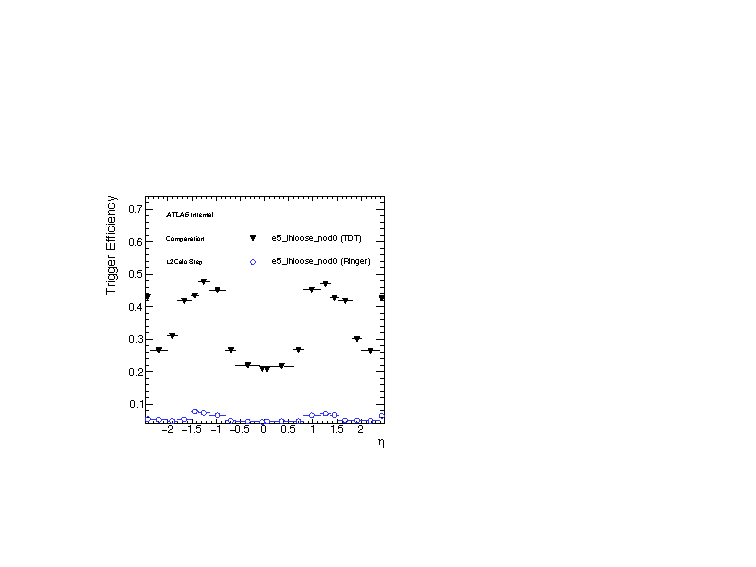
\includegraphics[width=.5\textwidth]{appendices/figures/low_et/e5_lhloose_eta_bkg}
  \caption{\label{fig:lowet_e5_lhloose_bkg}
\fastcalo{} background efficiency as a function of \eta{} for an electron
trigger requiring $\et > \SI{5}{\GeV}$ and \loose selection with (blue) and
without (black) the \rnn algorithm. Samples are selected with \Jee{} \tnp{} and
efficiencies are measured with full 2017 data employing the TriggerDecisionTool
(TDT) framework for the trigger without \rnn{}. The full trigger selection is
emulated on the same samples with the TriggerEmulationTool framework to allow
estimating the efficiency of the trigger with \rnn{}.
}
\end{figure}

\begin{figure}[htb]
\begin{center}
\begin{subfigure}[c]{.48\textwidth}
\centering
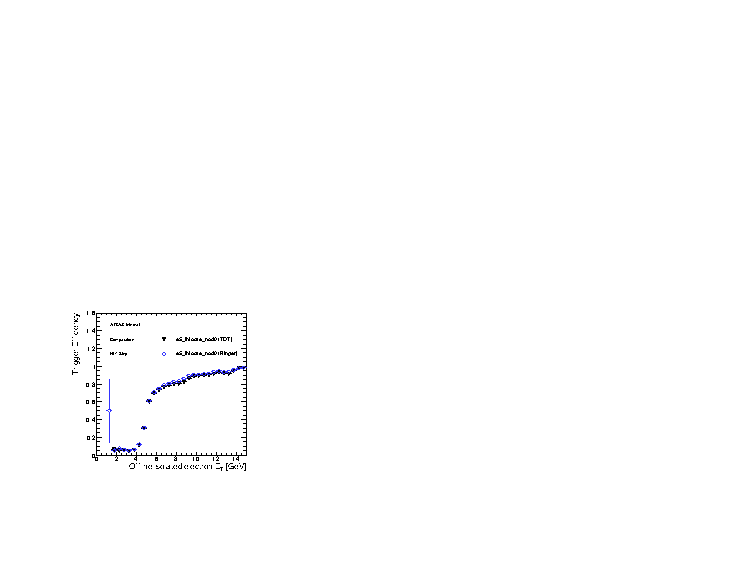
\includegraphics[width=\textwidth]{appendices/figures/low_et/e5_lhloose_et}
\caption{}
\label{fig:lowet_comp_et}
\end{subfigure}
\hfill
\begin{subfigure}[c]{.48\textwidth}
\centering
\includegraphics[width=\textwidth]{appendices/figures/low_et/e5_lhloose_eta}
\caption{}
\label{fig:lowet_comp_eta}
\end{subfigure} \\
\begin{subfigure}[c]{.48\textwidth}
\centering
\includegraphics[width=\textwidth]{appendices/figures/low_et/e5_lhloose_mu}
\caption{}
\label{fig:lowet_comp_mu}
\end{subfigure}
%\hfill
\caption{HLT electron efficiency as a function of \et{} (a), \eta{} (b) and \avgmu{}
(c) for an electron trigger requiring $\et > \SI{5}{\GeV}$
and \loose selection with (blue) and without (black) the \rnn algorithm. Details
on the efficiency measurement are described in
Figure~\ref{fig:lowet_e5_lhloose_bkg}.
}%
\label{fig:lowet_e5_lhloose}
\end{center}
\end{figure}

\FloatBarrier
\subsection{\rnn{} based only on ECAL Information}%
\label{ssec:ecal_rnn}

Another limitation for online operation is the trigger system readout
capability. Particularly, the readout rate of the \hcal{} cells is more likely
to reach its limitations given the hadronic pile-up nature and the their coarser
granularity. Some electron triggers, as those dedicated to cover
\BeeK{} decays, may be executed on top of the full \licalo{}
rate. A main challenge for these triggers during Run~2 was the \hcal{} readout
rate, which triggered the interest of developing an electron selection based only
in the \ecal{} information~\cite{ATR-18724}. It may be noticed that for low
kinematic operation (i.e. $\et<\SI{15}{\GeV}$) the signal-to-noise ratio in the
\hcal{} is lower due to pile-up contamination and, thus, may not be as useful as
for the selection of higher \et{} physics objects.

When investigating how much the hadronic information was beneficial to the
selector at the low kinematic region (Table~\ref{tab:comp_ecal_rnn}), we
observed that the \rnn{} operating with only \ecal{} information can bring
similar improvements with respect to the cut-based strategy. Depending on the
working point, a reduction of 25--50$\;$\% with respect to triggering without
\rnn{} can be obtained in the \fastcalo{} fake rate, while keeping the same
signal efficiency. If needed to keep the full \rnn{} efficiency, a possible
strategy could be to apply a two step \fastcalo selection, starting with the
\ecal{} and then applying the full \rnn{} decision. Finally, the \BeeK{} trigger
requires \rnn{} to handle boosted physics structure, which is part of the open
topics (Section~\ref{ssec:boosted_topology}).

\begin{table}[htb]
  \centering
  \includegraphics[width=.65\textwidth]{appendices/figures/low_et/nodhad_comparison_with_cutbased}
  \caption{Algorithm efficiencies for each working point using joint 2017 and
    2018 data as described in Section~\ref{ssec:low_et}. The fraction of fake
    rate reduction with respect to the cut-based algorithm is shown in red.
    `noHAD' is used to flag the \rnn{} algorithm accessing only \ecal{}
    information, whereas `100 rings' is the standard version of the \rnn{}.
  \label{tab:comp_ecal_rnn}}
\end{table}

%\subsection{Fudge Factors}%
%\label{ssec:fudge_factors}
% TriggerEgammaMeeting_20180213

\subsection{Lumiblocks with Inconsistent Trigger Efficiency}\label{ssec:lbs_lower_eff}
%/Users/wsfreund/Documents/Pesquisa/HEP/CERN/ID/Online/impact_on_lhpdfs/2017data/e28/runsSummaryLB_e28.pdf

By evaluating the number of \Zee{} \tnp{} pairs as in
Figure~\ref{fig:tap_pairs_count}, it is possible to observe some luminosity
blocks (LBs) where the trigger collect potentially less pairs than what was 
expected\footnote{The particular plot may be interesting to be implemented for
online and data quality monitoring. For instance, Figure~\ref{fig:run335282}
shows some LBs within the GRL where the \Zee{} \tnp{} electron trigger
efficiency was very low and may be worth the investigation for data quality
purposes.}.  Particularly, the LBs 113--136 in run 327636
(Figure~\ref{fig:run327636}), the range near 100--180 in run 328636
(Figure~\ref{fig:run328636}) and near 120--160 in run 331975
(Figure~\ref{fig:run331975}) show lower number of pairs with respect to the
other LBs for both duplicated triggers. For the particular regions, the trigger
with \rnn{} has a slightly lower number of pairs with respect to the its
cut-based counterpart. Investigating these data might improve the detection of
possible detector anomalies, but also it brings insights of the particularities
between the algorithms. Likewise, LBs 501, 751 and 790 in run 334779
(Figure~\ref{fig:run334779}) might be showing a systematic behavior where the
trigger with \rnn{} has higher efficiency than its counterpart.


\begin{figure}[b]
  \centering
\begin{subfigure}[c]{.49\textwidth}
\includegraphics[width=\textwidth]{appendices/figures/pairs_wrt_lb/run327636}%
\caption{\label{fig:run327636}}
\end{subfigure}
\hfill
\begin{subfigure}[c]{.49\textwidth}
\centering
\includegraphics[width=\textwidth]{appendices/figures/pairs_wrt_lb/run328263}%
\caption{\label{fig:run328636}}
\end{subfigure} \\
%\end{figure}
%\begin{figure}[t]\ContinuedFloat
\centering
\begin{subfigure}[c]{.49\textwidth}
\centering
\includegraphics[width=\textwidth]{appendices/figures/pairs_wrt_lb/run331975}%
\caption{\label{fig:run331975}}
\end{subfigure}
\hfill
\begin{subfigure}[c]{.49\textwidth}
\includegraphics[width=\textwidth]{appendices/figures/pairs_wrt_lb/run334779}%
\caption{\label{fig:run334779}}
\end{subfigure} \\
\begin{subfigure}[c]{.30\textwidth}
\centering
\includegraphics[width=\textwidth]{appendices/figures/pairs_wrt_lb/run335282}%
\caption{\label{fig:run335282}}
\end{subfigure}
\caption{\label{fig:tap_pairs_count}
Number of \Zee{} \tnp{} pairs collected by the duplicated trigger with (blue)
and without (black) \rnn{} per luminosity block in the good run list (GRL)
for five runs (from (a) to (e)) along 2017 data-taking.
}
\end{figure}

%\FloatBarrier{}
%\subsection{On-going Evaluations on the Quadrant Analysis}\label{ssec:quadrant_combined}
%
%An asymmetry can be observed in \deltaeta{} when we consider the
%disagreement profiles (Figure~\ref{fig:trigger_quadrant_deltaEta}), where the
%trigger with (without) \rnn{} is biased towards collecting more samples with
%negative (positive) value. This behavior only happens for the
%$0.6<\abseta{}<0.8$ region.
%
%\rnn{} trigger also displays a slightly less pronounced tail in \deltaphi{}
%(Figure~\ref{fig:trigger_quadrant_deltaPhi}).  Hence, there is some correlation
%level between this variable and the shower development information being
%explored by the \rnn{} algorithm.
%
%\begin{figure}[h!tb]
%\begin{subfigure}[c]{.49\textwidth}
%\includegraphics[width=\textwidth]{quadrant_plots/HLT_e28_lhtight_nod0_noringer_ivarloose_HLT_e28_lhtight_nod0_ivarloose_deltaEta1_et4_eta1.pdf}%
%\caption{\label{fig:trigger_quadrant_deltaEta}}
%\end{subfigure}
%\hfill
%\begin{subfigure}[c]{.49\textwidth}
%\centering
%\includegraphics[width=\textwidth]{quadrant_plots/HLT_e28_lhtight_nod0_noringer_ivarloose_HLT_e28_lhtight_nod0_ivarloose_deltaPhiRescaled2_et4_eta1.pdf}%
%\caption{\label{fig:trigger_quadrant_deltaPhi}}
%\end{subfigure} \\
%\caption{\label{fig:quadrant_combined_variables_30GeV}
%Quadrant analysis plots for the offline-reconstructed ID-calorimeter combined
%variables employed in the likelihood for the $0.6<\abseta{}<0.8$ and
%$30<\et{}~[\text{GeV}]<35$ slice.
%}
%\end{figure}
%
\FloatBarrier
\subsection[Supplementary Agreement Analysis]{Supplementary Agreement
Analysis\footnote{Figures shown in this section may not contain the
`\textbf{ATLAS} \emph{Internal}' label as the only version available was
created to be part of a PhD thesis but we emphasize that these figures have
not been approved as ATLAS public plots. Their regeneration to include the
internal flag is not straightforward.}}\label{ssec:supplementary_agreement}


Current tools available in physics data analysis frameworks provide statistical
tests that, although they have not been designed to the conditions of the
agreement analysis, can provide some useful insights. We take advantage of these
tests in one approach complementary to the homogeneity test presented in
Section~\ref{ssec:agreement}. Additionally, we develop a simple approach based
on pseudo-experiments with ``Toy'' Monte Carlo. Such complementary studies
comply with the ATLAS statistical guideline~\cite{atlas_recommendations_stats}:

\begin{quote}
\textbf{Recommendation}: Use multiple statistical techniques. When they agree
we are in ‘asymptopia’; when they disagree we learn something.
\end{quote}

The first supplementary strategy goes in a similar direction of the baseline
evaluation (Section~\ref{top:agreement_homogeneity_results}) but, instead of
splitting data into two groups, we obtain the profiles for the two trigger
configurations for the full dataset. We approach the problem as a
goodness-of-fit problem by assuming the trigger without the \rnn{} algorithm as
a model to explain the observations obtained in the histogram built from the
trigger with the \rnn{} algorithm. For evaluating the goodness-of-fit, we employ
the Kolmogorov-Smirnov (KS)~\cite{kendalls_vol1} and
$\chi^2$~\cite{guide_to_chisquared} tests.

The small differences in efficiency between the triggers result in fluctuations
in the number of probes in the histograms (see
Appendixes~\ref{top:homogeneity_extra} and~\ref{top:gof_extra}). Instead
reweighing the histograms to have the same mass, we preferred to keep the
original histograms and compute the expected $\chi_{i,j}^{s}$ residuals by

\begin{equation}
  \frac{\mu_{i,j}}{\sigma_{ref}} = \frac{\left(r_j - b_j\right) \times
  \frac{b_{i,j}}{b_i}}{\sigma_{b_{i,j}}},
  \label{eq:expected_residual}
\end{equation}

\noindent where $r_j$ and $b_j$ are the total number of observations in the
$j$th histograms obtained with and without ringer. $\sigma_{b_{i,j}}$ will be
employed as a unit for measuring the residuals. In order to benefit from
Gaussian error approximation ($\sigma_{b_{i,j}}\approx\sqrt{b_{i,j}}$), we
employed the conservative recommendations in~\cite{knoll} by grouping the
histogram bins to have a minimum count of 30 units. Results are available in
Section~\ref{top:agreement_gof_results}.

Finally, we dedicate to the direct evaluation of possible distortions in the
profiles by considering only the disjoint cases where the triggers with and
without \rnn{} disagree. To consider the dependency of the duplicated
trigger pair, we adopted a pseudo-experiment strategy using simulation.
Considering that both disjoint histograms come from the same population, we can
estimate the original profile based on maximum
likelihood as~\cite{chi_squared_comparing_hists}

\begin{equation}
  \hat{p_{i,j}}=\frac{r_{i,j}+b_{i,j}}{r_i+b_i},
\end{equation}

\noindent where $r_i$ ($b_i$) represent the total observed entries of the
histogram built with data collected by the trigger with (without) \rnn{} in the
$i$th $\et{}\times\eta{}$ axis region.

% FIXME quote the number of pseudo-experiments (i.e. arXiv:1005.1891v3)

We generate $10^5$ pseudo-experiments using the estimated
probabilities and total histogram counts to compute the Kullback-Leibler
divergence (\dkl{})~\cite{2009_cichocki_nonnegative}

\begin{equation}
\dkl(p_i||q_i) = \sum\limits_{j} (p_{i,j}-q_{i,j})\ln\left(\frac{p_{i,j}}{q_{i,j}}\right),
\end{equation}

\noindent where $p$ and $q$ are distributions for each variable obtained when
employing respectively the trigger with and without the \rnn{} selection and
approximated with the empirical frequency values  The $j$th individual
contributions computed to obtain the \dkl{} are kept in order to allow
evaluation of the regions bringing larger profile distortions.  We address the
results in Section~\ref{top:agreement_pseudo_results}.

\subsubsection{Goodness-of-Fit Results}\label{top:agreement_gof_results}

Figure~\ref{fig:gof_calo} show the residuals for the goodness-of-fit approach.
When comparing it with Figure~\ref{fig:groups_homogeneity_calo},
it can be observed that the goodness-of-fit approach show much lower
residual fluctuations. Namely, for the goodness-of-fit setup, the typical
fluctuations are of $\pm$\SI{0.2}{$\sigma$} around the expected residuals due to
small alteration in the trigger efficiency for their configuration (in the
particular region, slightly lower than the trigger without \rnn{}), whereas for
the homogeneity setup residuals of up to $\pm$\SI{4}{$\sigma$} can be observed.
The smaller residuals in the goodness-of-fit are caused by the difference in the
setup employed for collecting the samples. Usually, the two profiles are
collected separately, as in the homogeneity setup, in a scenario close to
independent and identically distributed (i.i.d.) sampling. Particularly, the
fluctuations are also expected to be Gaussian in this setup. In the
goodness-of-fit approach, however, the samples come from a \emph{single}
observation group which is subject to two distinct sample damaging
processes~\cite{rao1965discrete} which represent the triggers. Unlike the
i.i.d.\@ sampling, we are subject to having the \emph{exact} same samples
composing the two profiles.

Particularly, the triggers are expected to be highly correlated, as they are
designed to perform the same task with a similar pipeline. Hence, the fraction
of exact same samples in both profiles is expected to be large and, even in the
disagreement cases, some level of statistical dependency between the algorithms
can be obtained from the variables describing the shower development.
In fact, ignoring the statistical dependency between the algorithms is to assume
that the variables will not display any systematic difference between the two
algorithms.

The statistical hypothesis assumed by the KS and $\chi^2$ tests
ignore such dependency. We obtain a p-value of 1 for both tests in all
variables and regions (Appendix~\ref{top:gof_extra}), even when not reweighing
the profiles to account for the small changes in efficiencies. In other words,
the statistical and possible systematic fluctuations are too small with respect
to the expectations under the conditions assumed by the tests. Regardless of the
flaws in the tests, it allows us to highlight that any discussion concerning the
systematic impact of the configuration is bounded to a regime lower to
the expected statistical fluctuations in goodness-of-fit tests. For these tests,
the hypothesis holding is that both profiles are statistically identical.

Interestingly enough, it is possible to get some hints of deviations in the
profile by careful examination of the residuals in Figure~\ref{fig:gof_calo}.
Particularly, the profile of the trigger with the \rnn{} shows a slight shift
towards unitary \reta{}, \rphi{} and \eratio{} (i.e.\@ residuals above the
expectations in the right tail and below in the left tail). Likewise, the
profiles might also display a shift towards null \rhad{}, but it is difficult to
get any insight for \weta{}, \fI{} and \fIII{}. In order to further investigate
these effects, we dedicated to a deeper assessment available in
Section~\ref{top:agreement_pseudo_results}.

\begin{figure}[b]
\begin{center}
\begin{subfigure}[c]{.48\textwidth}
\centering
\includegraphics[width=\textwidth]{appendices/figures/noAdjustment/marginal_nosplit/e28_MergedRuns/base_new/el_reta_et40eta0_00_sigma_base_new.pdf}
\caption{}%
\label{fig:gof_reta}
\end{subfigure}
\hfill
\begin{subfigure}[c]{.48\textwidth}
\centering
\includegraphics[width=\textwidth]{appendices/figures/noAdjustment/marginal_nosplit/e28_MergedRuns/base_new/el_rphi_et40eta0_00_sigma_base_new.pdf}
\caption{}%
\label{fig:gof_rphi}
\end{subfigure} \\
\begin{subfigure}[c]{.48\textwidth}
\centering
\includegraphics[width=\textwidth]{appendices/figures/noAdjustment/marginal_nosplit/e28_MergedRuns/base_new/el_eratio_et40eta0_00_sigma_base_new.pdf}
\caption{}%
\label{fig:gof_eratio}
\end{subfigure}
\hfill
\begin{subfigure}[c]{.48\textwidth}
\centering
\includegraphics[width=\textwidth]{appendices/figures/noAdjustment/marginal_nosplit/e28_MergedRuns/base_new/el_rhad_et40eta0_00_sigma_base_new.pdf}
\caption{}%
\label{fig:gof_rhad}
\end{subfigure} \\
\end{center}
\end{figure}%
\begin{figure}[t]\ContinuedFloat
\begin{center}
\hspace*{\fill}
\begin{subfigure}[c]{.48\textwidth}
\centering
\includegraphics[width=\textwidth]{appendices/figures/noAdjustment/marginal_nosplit/e28_MergedRuns/base_new/el_weta2_et40eta0_00_sigma_base_new.pdf}
\caption{}%
\label{fig:gof_weta}
\end{subfigure}
\hspace*{\fill} \\
\begin{subfigure}[c]{.48\textwidth}
\centering
\includegraphics[width=\textwidth]{appendices/figures/noAdjustment/marginal_nosplit/e28_MergedRuns/base_new/el_f1_et40eta0_00_sigma_base_new.pdf}
\caption{}%
\label{fig:gof_f1}
\end{subfigure}
\hfill
\begin{subfigure}[c]{.48\textwidth}
\centering
\includegraphics[width=\textwidth]{appendices/figures/noAdjustment/marginal_nosplit/e28_MergedRuns/base_new/el_f3_et40eta0_00_sigma_base_new.pdf}
\caption{}%
\label{fig:gof_f3}
\end{subfigure} \\
\caption{%
Top: Histogram profiles for the calorimetry variables employed in the offline
likelihood in the $\et>\SI{40}{\GeV}$ and $0.00<\abseta{}<0.80$ regions using
the trigger without \rnn{} (blue area) and the trigger with \rnn{} (black line).
Bottom: residual contributions using as statistics $\chi^s$
(equation~\ref{eq:signed_chi}, in black) and the expected model for no
distortion (equation~\ref{eq:expected_residual}) w.r.t.\@ the reference.
}%
\label{fig:gof_calo}
\end{center}
\end{figure}

\FloatBarrier
\subsubsection{Pseudo-Experiment Results}\label{top:agreement_pseudo_results}

Both homogeneity and goodness-of-fit tests showed that any alteration in the
profiles due to systematic effects coming from trigger configuration are
negligible with respect to the magnitude of statistical fluctuations. In this
section, we dedicate to studying the cases where the triggers \emph{disagree} in
order to get more insight on their systematic impact in the derivation of the
likelihood pdfs regardless of its relevance.

Despite the usage of full 2017 data and the disagreement between the two
triggers, the homogeneity hypothesis for most variables (\rphi{} \fI{},
\eratio{} and \weta{}) is not rejected at a 0.05 confidence level. It shows that
the overall alteration in the profiles due to the trigger configuration is not
statistically strong for these variables even when considering only the
disagreement samples. Particularly, that is not the case for the \reta{} and
\rhad{} variables where the homogeneity hypothesis is discarded. For \reta{}, it
is possible to observe that the trigger with \rnn{} is likely to collect
more \tnp{} pairs with probe samples whose \reta{} values are greater than 0.959
and less otherwise with respect to triggering without it. Similarly, the trigger
with \rnn{} seems to be biased to collect less samples with \rhad{} above
values around \SI{1.75}{\textperthousand} and more otherwise with respect to its
duplicated counterpart. Although not being statistically significant, a similar
behavior may be present in \eratio{} and \rphi{}, where \rnn{} trigger displays
a slight shift toward unitary values.

Interestingly, these results are similar to those found in the quadrant analysis
(Section~\ref{top:quadrant_results}).  However, the reason for the single
electron trigger selection configuration applied on the tag to affect the probe
profiles is unclear. One possible explanation would be some correlation level
between the ID variables of the two Z electrons.

\begin{figure}[hbt]
\begin{center}
\begin{subfigure}[c]{.48\textwidth}
\centering
\includegraphics[width=\textwidth]{appendices/figures/noAdjustment/marginal_mutually_exclusive/e28_MergedRuns_mutuallyExclusive/bonly_nonly/el_reta_et40eta0_00_kldivergence_bonly_nonly.pdf}
\caption{}%
\label{fig:pseudo_reta}
\end{subfigure}
\hfill
\begin{subfigure}[c]{.48\textwidth}
\centering
\includegraphics[width=\textwidth]{appendices/figures/noAdjustment/marginal_mutually_exclusive/e28_MergedRuns_mutuallyExclusive/bonly_nonly/el_rphi_et40eta0_00_kldivergence_bonly_nonly.pdf}
\caption{}%
\label{fig:pseudo_rphi}
\end{subfigure} \\
\begin{subfigure}[c]{.48\textwidth}
\centering
\includegraphics[width=\textwidth]{appendices/figures/noAdjustment/marginal_mutually_exclusive/e28_MergedRuns_mutuallyExclusive/bonly_nonly/el_eratio_et40eta0_00_kldivergence_bonly_nonly.pdf}
\caption{}%
\label{fig:pseudo_eratio}
\end{subfigure}
\hfill
\begin{subfigure}[c]{.48\textwidth}
\centering
\includegraphics[width=\textwidth]{appendices/figures/noAdjustment/marginal_mutually_exclusive/e28_MergedRuns_mutuallyExclusive/bonly_nonly/el_rhad_et40eta0_00_kldivergence_bonly_nonly.pdf}
\caption{}%
\label{fig:pseudo_rhad}
\end{subfigure} \\
\end{center}
\end{figure}%
\begin{figure}[t]\ContinuedFloat
\begin{center}
\hspace*{\fill}
\begin{subfigure}[c]{.48\textwidth}
\centering
\includegraphics[width=\textwidth]{appendices/figures/noAdjustment/marginal_mutually_exclusive/e28_MergedRuns_mutuallyExclusive/bonly_nonly/el_weta2_et40eta0_00_kldivergence_bonly_nonly.pdf}
\caption{}%
\label{fig:pseudo_weta}
\end{subfigure}
\hspace*{\fill} 
\begin{subfigure}[c]{.48\textwidth}
\centering
\includegraphics[width=\textwidth]{appendices/figures/noAdjustment/marginal_mutually_exclusive/e28_MergedRuns_mutuallyExclusive/bonly_nonly/el_f1_et40eta0_00_kldivergence_bonly_nonly.pdf}
\caption{}%
\label{fig:pseudo_f1}
\end{subfigure}
\hfill
%\begin{subfigure}[c]{.48\textwidth}
%\centering
%\includegraphics[width=\textwidth]{noAdjustment/marginal_mutually_exclusive/e28_MergedRuns_mutuallyExclusive/bonly_nonly/el_f3_et40eta0_00_kldivergence_bonly_nonly.pdf}
%\caption{}%
%\label{fig:pseudo_f3}
%\end{subfigure} \\
\caption{The top pad shows the histogram profiles for the disagreements between
  triggering with and without \rnn{} for each calorimetry
  variable\footnotemark{} employed in the offline likelihood in the
  $\et>\SI{40}{\GeV}$ and $0.00<\abseta{}<0.80$ regions. Abscissa is weighed
  through the histogram bin size according to the bin-to-bin observed
  ($\dkl{}(b_{obs}||r_{obs})$) divergence contributions, shown in orange in the
  bottom pad. They are computed for each bin by the divergence between triggers
  with \rnn{} (square in the top pad) and without (circle). The triangles show
  the observations of the trigger with \rnn{} reweighed to have the same mass of
  the other trigger.  On the top left, the observed \dkl{} between the two
  profiles is shown in the red line.  The mean and standard deviation of the
  pseudo-experiment \dkl{} distribution followed by the corresponding p-value is
  in the next line. The unidimensional distribution of the pseudo-experiments
  are in blue and red for each bin. The distribution for the bin-to-bin \dkl{}
  contributions is in grey in the bottom pad. Dashed lines indicate the bin
  boundaries and the values on top are the corresponding bin centers.}%
\label{fig:pseudo_calo}
\end{center}
\end{figure}

\footnotetext{\fIII{} is not included due to technical issues.}

\FloatBarrier

%\include{sections/low_et}
%\section{Auxiliary Material}%
\label{sec:aux_mat}

This section contains auxiliary or record-keeping material.

\subsection{\itc Cells (TileGap)}%
\label{ssec:tilegap}

Figure~\ref{fig:tilecal_cells} displays the configuration of the \itc cells
which break the longitudinal layers concept employed in the \rnn algorithm.
These cells were employed in the ringer algorithm as described in
Table~\ref{tab:ring_alg_parameters}, as slight additional efficiency was
observed in the crack region during Run~1 developments.

\begin{figure}[h!t]
\centering
\includegraphics[width=\textwidth]{appendices/figures/tilegap.pdf}
\caption{Schematic slice of the barrel (left), extended barrel (right) and
  intermediate calorimeter (highlighted) cells of the \tilecal.}%
\label{fig:tilecal_cells}
\end{figure}

\FloatBarrier{}
\newpage
\subsection{MLP Output for Simulated and Collision Data}\label{ssec:mcdata_nnoutput}

Figure~\ref{fig:mcdata_nnoutput} shows the effect of simulation mis-modellings
in the MLP output, where a shift towards negative values (more background-like)
are seen for both signal and background data. We did not employ pile-up
reweighing tools on MC data for the generation of these plots, hence the
profiles are observed with different pile-up conditions.

\begin{figure}[ht]
  \centering
\includegraphics[width=0.8\textwidth]{appendices/figures/nn_output_mc15_versus_data16_et2_eta0.pdf}
\caption{MLP outputs for 2017 \rnn{} tunes for 
regions $30 < \et{} [\GeV] < 40$ and $0.0 < |\eta| < 0.8$ slice.\label{fig:mcdata_nnoutput}.}
\end{figure}


\subsection{MLP Topology}
\label{ssec:mlp_topo}

We should include some description here.




\begin{table}[ht!]
\scriptsize
\resizebox{1.000000\textwidth}{!}{%
\begin{tabular}
{lccccccc}
\hline
\hline
&  & $15 < E_{T} \text{[Gev]}<20$ & $20 < E_{T} \text{[Gev]}<30$ & $30 < E_{T} \text{[Gev]}<40$ & $40 < E_{T} \text{[Gev]}<50$ & $E_{T}\text{[GeV]} > 50$ \\
\hline
\multirow{3}{*}{$0.00<\eta<0.80$} & Input & 100 & 100 & 100 & 100 & 100 \\
& Hidden & \cellcolor[HTML]{9AFF99}5 & \cellcolor[HTML]{9AFF99}5 & \cellcolor[HTML]{9AFF99}5 & \cellcolor[HTML]{9AFF99}5 & \cellcolor[HTML]{9AFF99}5 \\
& Output & 1 & 1 & 1 & 1 & 1 \\
\hline
\multirow{3}{*}{$0.80<\eta<1.37$} & Input & 100 & 100 & 100 & 100 & 100 \\
& Hidden & \cellcolor[HTML]{9AFF99}5 & \cellcolor[HTML]{9AFF99}5 & \cellcolor[HTML]{9AFF99}5 & \cellcolor[HTML]{9AFF99}5 & \cellcolor[HTML]{9AFF99}5 \\
& Output & 1 & 1 & 1 & 1 & 1 \\
\hline
\multirow{3}{*}{$1.37<\eta<1.54$} & Input & 100 & 100 & 100 & 100 & 100 \\
& Hidden & \cellcolor[HTML]{9AFF99}7 & \cellcolor[HTML]{9AFF99}19 & \cellcolor[HTML]{9AFF99}13 & \cellcolor[HTML]{9AFF99}13 & \cellcolor[HTML]{9AFF99}6 \\
& Output & 1 & 1 & 1 & 1 & 1 \\
\hline
\multirow{3}{*}{$1.54<\eta<2.50$} & Input & 100 & 100 & 100 & 100 & 100 \\
& Hidden & \cellcolor[HTML]{9AFF99}5 & \cellcolor[HTML]{9AFF99}15 & \cellcolor[HTML]{9AFF99}5 & \cellcolor[HTML]{9AFF99}5 & \cellcolor[HTML]{9AFF99}5 \\
& Output & 1 & 1 & 1 & 1 & 1 \\
\hline
\hline
\end{tabular}
}
\caption{Number of neuron in hidden layer for 2017 operation.}
\label{tab:neurons_v6}
\end{table}


\begin{table}[ht!]
    \scriptsize
    \resizebox{1.000000\textwidth}{!}{%
    \begin{tabular}
    {lccccccc}
    \hline
    \hline
    &  & $15 < E_{T} \text{[Gev]}<20$ & $20 < E_{T} \text{[Gev]}<30$ & $30 < E_{T} \text{[Gev]}<40$ & $40 < E_{T} \text{[Gev]}<50$ & $E_{T}\text{[GeV]} > 50$ \\
    \hline
    \multirow{3}{*}{$0.00<\eta<0.80$} & Input & 100 & 100 & 100 & 100 & 100 \\
    & Hidden & \cellcolor[HTML]{9AFF99}5 & \cellcolor[HTML]{9AFF99}5 & \cellcolor[HTML]{9AFF99}5 & \cellcolor[HTML]{9AFF99}5 & \cellcolor[HTML]{9AFF99}5 \\
    & Output & 1 & 1 & 1 & 1 & 1 \\
    \hline
    \multirow{3}{*}{$0.80<\eta<1.37$} & Input & 100 & 100 & 100 & 100 & 100 \\
    & Hidden & \cellcolor[HTML]{9AFF99}5 & \cellcolor[HTML]{9AFF99}5 & \cellcolor[HTML]{9AFF99}5 & \cellcolor[HTML]{9AFF99}5 & \cellcolor[HTML]{9AFF99}5 \\
    & Output & 1 & 1 & 1 & 1 & 1 \\
    \hline
    \multirow{3}{*}{$1.37<\eta<1.54$} & Input & 100 & 100 & 100 & 100 & 100 \\
    & Hidden & \cellcolor[HTML]{9AFF99}5 & \cellcolor[HTML]{9AFF99}5 & \cellcolor[HTML]{9AFF99}5 & \cellcolor[HTML]{9AFF99}5 & \cellcolor[HTML]{9AFF99}5 \\
    & Output & 1 & 1 & 1 & 1 & 1 \\
    \hline
    \multirow{3}{*}{$1.54<\eta<2.37$} & Input & 100 & 100 & 100 & 100 & 100 \\
    & Hidden & \cellcolor[HTML]{9AFF99}5 & \cellcolor[HTML]{9AFF99}5 & \cellcolor[HTML]{9AFF99}5 & \cellcolor[HTML]{9AFF99}5 & \cellcolor[HTML]{9AFF99}5 \\
    & Output & 1 & 1 & 1 & 1 & 1 \\
    \hline
    \multirow{3}{*}{$2.37<\eta<2.50$} & Input & 100 & 100 & 100 & 100 & 100 \\
    & Hidden & \cellcolor[HTML]{9AFF99}5 & \cellcolor[HTML]{9AFF99}5 & \cellcolor[HTML]{9AFF99}5 & \cellcolor[HTML]{9AFF99}5 & \cellcolor[HTML]{9AFF99}5 \\
    & Output & 1 & 1 & 1 & 1 & 1 \\
    \hline
    \hline
    \end{tabular}
    }
    \caption{Number of neuron in hidden layer for 2018 operation.}
    \label{tab:neurons_v8}
    \end{table}
    



\subsection{Monitoring Histograms of \fastcalo Algorithms Total CPU
Time}\label{ssec:fastcalo_monitoring}

During Run~2, \fastcalo feature extraction algorithm executed sequentially the
following tools: ESamp2 (EM2 shower shapes), ESamp1 (EM1 shower shapes), EaEm
(raw EM energy) and EHadEn (raw HAD energy). The CPU time obtained using the
monitoring tool for the electron trigger without \rnn are available in
Figure~\ref{fig:fastcalo_fex_tools_time}.

\begin{figure}[ht]
\begin{subfigure}[c]{.48\textwidth}
\includegraphics[width=\textwidth]{appendices/figures/fastcalo_time/samp2.pdf}
\centering
\end{subfigure}
\begin{subfigure}[c]{.48\textwidth}
\includegraphics[width=\textwidth]{appendices/figures/fastcalo_time/samp1.pdf}
\centering
\end{subfigure} \\
\begin{subfigure}[c]{.48\textwidth}
\includegraphics[width=\textwidth]{appendices/figures/fastcalo_time/ementotal.pdf}
\centering
\end{subfigure}
\begin{subfigure}[c]{.48\textwidth}
\includegraphics[width=\textwidth]{appendices/figures/fastcalo_time/ehadtotal.pdf}
\centering
\end{subfigure}
\caption{CPU time in the monitoring tool for each \fastcalo tool (except for
calibration). The histograms are shown for the electron trigger without \rnn.
Measurement configuration is described in Figure~\ref{fig:fastcalo_fex_time}.}%
\label{fig:fastcalo_fex_tools_time}
\end{figure}

\subsection{Multi-modal CPU time structure of ESamp2 Algorithm}\label{ssec:esamp2}

The multi-modal distribution observed in ESamp2 total CPU time
(Figure~\ref{fig:fastcalo_fex_tools_time}) is mainly
(Figure~\ref{fig:fastcalo_samp2_contributions}) due to the retrieval of
the EM2 cells information (ESamp2BSCnv), but also observed in ESamp2Reg with
lower central values. The two peaks around \SI{0.7}{\ms/\text{event}} and
\SI{0.9}{\ms/\text{event}} are one of the largest contributions to the total
\fastcalo CPU time.

\begin{figure}[ht]
\begin{subfigure}[c]{.48\textwidth}
\includegraphics[width=\textwidth]{appendices/figures/fastcalo_time/ESamp2BSCnv.pdf}
\centering
\end{subfigure}
\begin{subfigure}[c]{.48\textwidth}
\includegraphics[width=\textwidth]{appendices/figures/fastcalo_time/ESamp2Reg.pdf}
\centering
\end{subfigure} \\
\centering
\caption{CPU time of particular computations in the ESamp2 algorithm. The
histograms are shown for the electron trigger without \rnn.  Measurement
configuration is described in Figure~\ref{fig:fastcalo_fex_time}.}%
\label{fig:fastcalo_samp2_contributions}
\end{figure}

\FloatBarrier

%\subsection{Lowest-Threshold Unprescaled Isolated Single-Electron Trigger Rate
%with respect to Luminosity}\label{ssec:primary_rate_wrt_luminosity}
%
%Figure~\ref{fig:primary_trigger_rate_wrt_lumi} shows similar trigger rates with
%respect to instantaneous luminosity for the period 2015--2018.
%
%\begin{figure}[t]
%  \centering
%  \includegraphics[width=.6\textwidth]{public_plots/fig_14}
%  \caption{\label{fig:primary_trigger_rate_wrt_lumi}Dependence of the trigger
%  rate on the luminosity for the lowest-threshold unprescaled isolated
%single-electron triggers in 2015--2018.}
%\end{figure}
%
\subsection{Background Efficiency Measurement for 2017
Cost Monitoring}\label{ssec:2017_cost_background_eff}

Estimations using the cost monitoring duplicated triggers in different
runs are shown in Table~\ref{tab:results_commissioning_v6_cost_monitoring}.
\rnn improvements range from 1.5 to 5$\times$\footnote{Specifically
for the configuration and trigger evaluated on
Figure~\ref{fig:fastcalo_fex_time}, a 1.5$\times$ reduction factor is obtained.}
and are dependent on both the trigger \et and selection requirements.

\begin{table}[ht!]
    \centering
    \caption{\label{tab:results_commissioning_v6_cost_monitoring}%
    Total number of \fastcalo and \fastelectron executions requested per monitored
    trigger in CPU cost evaluations ATR-16656 (run 309640) and ATR-16657 (run
    327265) using the final 2017 \rnn configuration and evaluated in the nightly release
    AtlasP1-21.1-2017-07-01. The reduction factor is computed as the fraction of
    \fastelectron executions in previous trigger (without \rnn) with respect to
    proposed trigger (with \rnn). See~\cite{Pinto2017} for more details.
    }
    \resizebox{\textwidth}{!}{%
    \begin{tabular}{%
    llr
    S[table-format=4.0, table-number-alignment=center,
    round-mode=figures, round-precision=2]
    c
    }
    \hline \hline
    run &
    \multirow{2}{*}{trigger} &
    %\begin{tabular}[c]{@{}c@{}}\fastcalo \\
    %(calls)\end{tabular}
    \multicolumn{1}{c}{\fastcalo} &
    \multicolumn{1}{c}{\fastelectron} &
    \multicolumn{1}{c}{Reduction} \\ \cline{3-4}
    \multicolumn{1}{c}{number} &
    &
    \multicolumn{2}{c}{Total Executions $\times 10^{-3}$ } &
    \multicolumn{1}{c}{Factor} \\
    \hline \hline
    \multirow{6}{*}{309640} & e17\_lhvloose\_nod0\_noringer\_L1EM15VHI &
    \multirow{2}{*}{\numRF{17989.136}{2}} & 8984.315 &
    \multicolumn{1}{c}{\multirow{2}{*}{1.71$\times$}} \\ \cline{4-4}
    
    & e17\_lhvloose\_nod0\_L1EM15VHI &  & 5234.167 &  \\ \cline{2-5}
    
    & e28\_lhtight\_nod0\_noringer\_ivarloose\_L1EM24VHIM &
    \multirow{2}{*}{\numRF{3084.292}{2}} & 1046.078 &
    \multicolumn{1}{c}{\multirow{2}{*}{1.69$\times$}} \\ \cline{4-4}
    
    & e28\_lhtight\_nod0\_ivarloose\_L1EM24VHIM &  & 618.011 &  \\ \cline{2-5}
    
    & e60\_lhmedium\_nod0\_noringer\_L1EM24VHIM & \multirow{2}{*}{\numRF{3084.292}{2}} &
    1046.078 & \multicolumn{1}{c}{\multirow{2}{*}{4.91$\times$}} \\ \cline{4-4}
    
    & e60\_lhmedium\_nod0\_L1EM24VHIM &  & 213.037 &  \\ \hline \hline
    
    \multicolumn{1}{l}{\multirow{6}{*}{327265}} &
    e17\_lhvloose\_nod0\_noringer\_L1EM15VHI & \multirow{2}{*}{\numRF{15609.134}{2}}
    & 7400.864 &
    \multicolumn{1}{c}{\multirow{2}{*}{1.52$\times$}} \\ \cline{4-4}
    
    \multicolumn{1}{l}{} & e17\_lhvloose\_nod0\_L1EM15VHI &  & 4855.326 &
    \multicolumn{1}{l}{} \\ \cline{2-5}
    
    \multicolumn{1}{l}{} & e28\_lhtight\_nod0\_noringer\_ivarloose\_L1EM24VHIM &
    \multirow{2}{*}{\numRF{3296.808}{2}} & 1150.932 &
    \multicolumn{1}{c}{\multirow{2}{*}{1.58$\times$}} \\ \cline{4-4}
    
    \multicolumn{1}{l}{} & e28\_lhtight\_nod0\_ivarloose\_L1EM24VHIM &  & 725.655 &
    \multicolumn{1}{l}{} \\ \cline{2-5}
    
    \multicolumn{1}{l}{} & e60\_lhmedium\_nod0\_noringer\_L1EM24VHIM &
    \multirow{2}{*}{\numRF{3296.808}{2}} & 238.054 &
    \multicolumn{1}{c}{\multirow{2}{*}{3.10$\times$}} \\ \cline{4-4}
    
    \multicolumn{1}{l}{} & e60\_lhmedium\_nod0\_L1EM24VHIM &  & 76.735 &
    \multicolumn{1}{l}{} \\ \hline \hline
    \end{tabular}%
    }
    \end{table}



\FloatBarrier
\subsection{2016 Emulated Results}%

Table~\ref{tab:results_commissioning_v6_emulation} shows emulated results during
development stage for both collision and simulation datasets.

\begin{table}[ht]
    \begin{center}
    %\captionof{table}{%
    \caption{%
    \label{tab:results_commissioning_v6_emulation} Emulated efficiency measurements
    of the trigger e26\_lhtight\_nod0 executed with and without \rnn using 2016 menu
    version. The denominator is common for all selection stages and is the number of
    RoIs matched to an electron object reconstructed by the offline. For
    uncertainties smaller than 0.01, only central values are shown. Simulated
    dataset employed Zee and JF17 mc15 datasets (AMI tag:
    \text{e3848\_s2876\_r7917\_r7676}) respectively for signal and background
    samples. Collision data are obtained from PhysicsMain and EnhancedBias streams
    using the selection criteria in Section~\ref{ssec:dataset}.}%
    \begin{tabular}{lcccc}
    \hline
    \hline
    \hline
    Chain & FastCalo [\%] & FastElectron [\%] & HLTCalo [\%] & HLT [\%] \\
    \hline \hline
    \multicolumn{5}{c}{Run 311244} \\
    \hline
    \hline
    \multicolumn{5}{c}{Signal Efficiency} \\
    \hline \hline
    Without \rnn & $96.77 \pm 0.03$ & $96.70 \pm 0.03$ & $95.84 \pm 0.05$ & $89.74 \pm 0.07 $ \\
    \hline
    With \rnn & $96.23 \pm 0.03$ & $96.16 \pm 0.03$ & $95.31 \pm 0.04$ & $89.32 \pm 0.08$ \\
    \hline
    \hline
    \multicolumn{5}{c}{Background Efficiency} \\
    \hline
    Without \rnn & $ 16.03 \pm 0.02 $ & $15.70 \pm 0.02$ & $12.90 \pm 0.02$ & $0.57$ \\
    \hline
    \hline
    With \rnn & $ 5.41 \pm 0.02$ & $5.12 \pm 0.02$ & $3.40 \pm 0.01$ & $ 0.54 $ \\
    \hline \hline
    \multicolumn{5}{c}{Simulation} \\
    \hline \hline
    \multicolumn{5}{c}{Signal Efficiency} \\
    \hline \hline
    Without \rnn & $ 96.10 \pm 0.01 $ & $ 96.09 \pm 0.01$ &
    $95.37 \pm 0.01 $ & $89.06 \pm 0.01 $ \\
    \hline
    With \rnn & $ 96.11 \pm 0.01 $ & $ 96.09 \pm 0.01$ &
    $95.38 \pm 0.01 $ & $89.12 \pm 0.01$ \\
    \hline
    \hline
    \multicolumn{5}{c}{Background Efficiency} \\
    \hline
    \hline
    Without \rnn & $8.04 \pm 0.01$ & $7.93 \pm 0.01$ & $6.54 $ &
    $0.20$ \\
    \hline
    With \rnn & $3.69 \pm 0.01$ & $3.59 \pm 0.01$ & $2.55 $ &
    $0.19$ \\
    \hline
    \hline
    \hline
    \end{tabular}
    \end{center}
    \end{table}

\FloatBarrier
\subsection{Agreement Analysis }%
\label{ssec:agreement_extra}

\subsubsection{Homogeneity Test}%
\label{top:homogeneity_extra}

Figure~\ref{fig:probe_groups} shows that using larger periods than consecutive
luminosity blocks resulted in a small difference in the total number of counts.
The absolute difference is bounded at \SI{1.5}{\%} but typically lower than
\SI{0.2}{\%}. Figures~\ref{fig:groups_homogeneity_id}
and~\ref{fig:groups_homogeneity_caloid} show the residuals for ID and calo-ID
combined variables, respectively. Tables~\ref{tab:p_values_homogeneity}
and~\ref{tab:p_values_homogeneity_track} show that the trigger configuration has
negligible impact in the homogeneity test p-values for the offline likelihood
variables.

\begin{sidewaysfigure}[ht]
  \centering
\begin{subfigure}[c]{.32\textwidth}
\centering
\includegraphics[width=\textwidth]{appendices/figures/noAdjustment/marginal_split/e28_SplitConsecutiveFiles/base_base/probe_count0_base_base.pdf}
\caption{}%
\label{fig:probe_group0_base}
\end{subfigure}
\begin{subfigure}[c]{.32\textwidth}
\centering
\includegraphics[width=\textwidth]{appendices/figures/noAdjustment/marginal_split/e28_SplitConsecutiveFiles/base_base/delta_perc_base_base.pdf}
\caption{}%
\label{fig:probe_delta_perc_base_base}
\end{subfigure}
\begin{subfigure}[c]{.32\textwidth}
\centering
\includegraphics[width=\textwidth]{appendices/figures/noAdjustment/marginal_split/e28_SplitConsecutiveFiles/base_base/probe_count1_base_base.pdf}
\caption{}%
\label{fig:probe_group1_base}
\end{subfigure} \\
\hspace*{\fill}
\begin{subfigure}[c]{.32\textwidth}
\includegraphics[width=\textwidth]{appendices/figures/noAdjustment/marginal_split/e28_SplitConsecutiveFiles/base_new/delta_perc_base_new.pdf}
\caption{}%
\label{fig:probe_delta_perc_base_new}
\end{subfigure}
\hspace*{\fill} \\
\begin{subfigure}[c]{.32\textwidth}
\centering
\includegraphics[width=\textwidth]{appendices/figures/noAdjustment/marginal_split/e28_SplitConsecutiveFiles/new_new/probe_count0_new_new.pdf}
\caption{}%
\label{fig:probe_group0_new}
\end{subfigure}
\begin{subfigure}[c]{.32\textwidth}
\centering
\includegraphics[width=\textwidth]{appendices/figures/noAdjustment/marginal_split/e28_SplitConsecutiveFiles/new_new/delta_perc_new_new.pdf}
\caption{}%
\label{fig:probe_delta_perc_new_new}
\end{subfigure}
\begin{subfigure}[c]{.32\textwidth}
\centering
\includegraphics[width=\textwidth]{appendices/figures/noAdjustment/marginal_split/e28_SplitConsecutiveFiles/new_new/probe_count1_new_new.pdf}
\caption{}%
\label{fig:probe_group1_new}
\end{subfigure} \\
\caption{\label{fig:probe_groups}Probe counts per phase space region for the
  arbitrary first (a,e) and second (c,g) groups. First (third) line concern the probes
obtained by the trigger without (with) \rnn{}. The difference percentage between
the two groups is shown in the middle column (b,d,f). In the second line (d),
the difference percentage is computed between probe counts in first group
collected by the trigger without \rnn{} and second group collected by the
trigger with \rnn{}.}
\end{sidewaysfigure}

\FloatBarrier

\begin{figure}[b]
\begin{center}
\begin{subfigure}[c]{.48\textwidth}
\centering
\includegraphics[width=\textwidth]{appendices/figures/noAdjustment/marginal_split/e28_SplitConsecutiveFiles/base_new/el_trackd0pvunbiased_et40eta0_00_sigma_base_new.pdf}
\caption{}%
\label{fig:groups_homogeneity_d0}
\end{subfigure}
\hfill
\begin{subfigure}[c]{.48\textwidth}
\centering
\includegraphics[width=\textwidth]{appendices/figures/noAdjustment/marginal_split/e28_SplitConsecutiveFiles/base_new/el_d0significance_et40eta0_00_sigma_base_new.pdf}
\caption{}%
\label{fig:groups_homogeneity_d0sig}
\end{subfigure} \\
\begin{subfigure}[c]{.48\textwidth}
\centering
\includegraphics[width=\textwidth]{appendices/figures/noAdjustment/marginal_split/e28_SplitConsecutiveFiles/base_new/el_DeltaPoverP_et40eta0_00_sigma_base_new.pdf}
\caption{}%
\label{fig:groups_homogeneity_poverp}
\end{subfigure}
\hfill
\begin{subfigure}[c]{.48\textwidth}
\centering
\includegraphics[width=\textwidth]{appendices/figures/noAdjustment/marginal_split/e28_SplitConsecutiveFiles/base_new/el_TRT_PID_et40eta0_00_sigma_base_new.pdf}
\caption{}%
\label{fig:groups_homogeneity_trt_pid}
\end{subfigure} \\
\end{center}
\caption{%
profiles for the calo-ID combined variables employed in
the offline likelihood in the $\et>\SI{40}{\GeV}$ and $0.00<\abseta{}<0.80$
region using data collected by trigger without \rnn{} in the first arbitrary
data group (blue area) and data collected by the trigger with \rnn{} in the
second arbitrary data group (black line).
}%
\label{fig:groups_homogeneity_id}
\end{figure}%

\begin{figure}[t]
\begin{center}
\begin{subfigure}[c]{.48\textwidth}
\centering
\includegraphics[width=\textwidth]{appendices/figures/noAdjustment/marginal_split/e28_SplitConsecutiveFiles/base_new/el_deltaeta1_et40eta0_00_sigma_base_new.pdf}
\caption{}%
\label{fig:groups_homogeneity_deta}
\end{subfigure}
\begin{subfigure}[c]{.48\textwidth}
\centering
\includegraphics[width=\textwidth]{appendices/figures/noAdjustment/marginal_split/e28_SplitConsecutiveFiles/base_new/el_deltaphiRescaled_et40eta0_00_sigma_base_new.pdf}
\caption{}%
\label{fig:groups_homogeneity_dphi}
\end{subfigure}
\caption{%
profiles for the calo-ID combined variables employed in
the offline likelihood in the $\et>\SI{40}{\GeV}$ and $0.00<\abseta{}<0.80$
region using data collected by trigger without \rnn{} in the first arbitrary
data group (blue area) and data collected by the trigger with \rnn{} in the
second arbitrary data group (black line).
}%
\label{fig:groups_homogeneity_caloid}
\end{center}
\end{figure}

\FloatBarrier

\begin{table}[b]
\centering
\caption{\label{tab:p_values_homogeneity}Homogeneity test p-value and cumulated
  $\chi^2/\text{ndf}$ for the calorimeter variables and $\et{}\times\eta{}$
  regions employed to derive the offline likelihood pdfs. The lines in blue,
  yellow and green correspond respectively to the results when computing the
  test between: the trigger without the \rnn{} for the two groups; trigger with
  \rnn{} for the first and without for the second group; and trigger with the
  \rnn{} for the two groups. }
\begin{subtable}{\textwidth}
\caption{\reta{}\label{tab:p_values_reta}}
\includegraphics[width=\textwidth]{appendices/figures/homogeneity/reta_homogeneity_table.pdf}
\end{subtable} \\
\begin{subtable}{\textwidth}
\caption{\rphi{}\label{tab:p_values_rphi}}
\includegraphics[width=\textwidth]{appendices/figures/homogeneity/rphi_homogeneity_table.pdf}
\end{subtable} \\
\begin{subtable}{\textwidth}
\caption{\eratio{}\label{tab:p_values_eratio}}
\includegraphics[width=\textwidth]{appendices/figures/homogeneity/eratio_homogeneity_table.pdf}
\end{subtable} \\
\end{table}%
\begin{table}[t]\ContinuedFloat\addtocounter{table}{-1}%
\begin{subtable}{\textwidth}
\caption{\rhad{}\label{tab:p_values_rhad}}
\includegraphics[width=\textwidth]{appendices/figures/homogeneity/rhad_homogeneity_table.pdf}
\end{subtable} \\
\begin{subtable}{\textwidth}
\caption{\weta{}\label{tab:p_values_weta}}
\includegraphics[width=\textwidth]{appendices/figures/homogeneity/weta2_homogeneity_table.pdf}
\end{subtable} \\
\begin{subtable}{\textwidth}
\caption{\fI{}\label{tab:p_values_f1}}
\includegraphics[width=\textwidth]{appendices/figures/homogeneity/f1_homogeneity_table.pdf}
\end{subtable} \\
\begin{subtable}{\textwidth}
\caption{\fIII{}\label{tab:p_values_f3}}
\includegraphics[width=\textwidth]{appendices/figures/homogeneity/f3_homogeneity_table.pdf}
\end{subtable} \\
\end{table}


\begin{table}[b]
\centering
\caption{\label{tab:p_values_homogeneity_track}Homogeneity test p-value and cumulated
  $\chi^2/\text{ndf}$ for the ID and calo-ID combined variables and $\et{}\times\eta{}$
  regions employed to derive the offline likelihood pdfs.}
\begin{subtable}{\textwidth}
\caption{\TRTPID{}\label{tab:p_values_trt}}
\includegraphics[width=\textwidth]{appendices/figures/homogeneity/TRT_PID_homogeneity_table.pdf}
\end{subtable} \\
\begin{subtable}{\textwidth}
\caption{\deltaeta{}\label{tab:p_values_eta}}
\includegraphics[width=\textwidth]{appendices/figures/homogeneity/deltaeta_homogeneity_table.pdf}
\end{subtable} \\
\begin{subtable}{\textwidth}
\caption{\deltaphires{}\label{tab:p_values_deltaphi}}
\includegraphics[width=\textwidth]{appendices/figures/homogeneity/deltaphi_homogeneity_table}
\end{subtable} \\
\end{table}
\begin{table}[t]\ContinuedFloat\addtocounter{table}{-1}
\begin{subtable}{\textwidth}
\caption{\deltapoverp{}\label{tab:p_values_poverp}}
\includegraphics[width=\textwidth]{appendices/figures/homogeneity/deltapoverp_homogeneity_table.pdf}
\end{subtable} \\
\begin{subtable}{\textwidth}
\caption{\trackdO{}\label{tab:p_values_d0}}
\includegraphics[width=\textwidth]{appendices/figures/homogeneity/d0_homogeneity_table.pdf}
\end{subtable} \\
\begin{subtable}{\textwidth}
\caption{\dOSignificance{}\label{tab:p_values_d0sig}}
\includegraphics[width=\textwidth]{appendices/figures/homogeneity/d0significance_homogeneity_table}
\end{subtable} \\
\end{table}

\FloatBarrier
\subsubsection{Goodness-of-fit}%
\label{top:gof_extra}

Figure~\ref{fig:gof_counts} shows that the absolute difference in number of
probes is bounded around \SI{0.3}{\%}.
Table~\ref{tab:gof_chi2_p_values} and~\ref{tab:gof_ks_p_values} show the results
for $chi^2$ and KS tests, respectively. The variables relying on ID information
are shown in Figure~\ref{fig:gof_track}.

\begin{figure}[b]
\begin{center}
\begin{subfigure}[c]{.48\textwidth}
\centering
\includegraphics[width=\textwidth]{appendices/figures/noAdjustment/marginal_nosplit/e28_MergedRuns/base_new/probe_count0_base_new.pdf}
\caption{}%
\label{fig:gof_counts_without_ringer}
\end{subfigure}
\begin{subfigure}[c]{.48\textwidth}
\centering
\includegraphics[width=\textwidth]{appendices/figures/noAdjustment/marginal_nosplit/e28_MergedRuns/base_new/probe_count1_base_new.pdf}
\caption{}%
\label{fig:gof_counts_with_ringer}
\end{subfigure} \\
\hspace*{\fill}
\begin{subfigure}[c]{.48\textwidth}
\centering
\includegraphics[width=\textwidth]{appendices/figures/noAdjustment/marginal_nosplit/e28_MergedRuns/base_new/delta_perc_base_new.pdf}
\caption{}%
\label{fig:gof_delta_perc}
\end{subfigure}
\hspace*{\fill} \\
\caption{%
  Probe counts per phase space region for the trigger with (a) and without (b)
  \rnn{}. The difference percentage between the two triggers is shown at the
  bottom (c).
}%
\label{fig:gof_counts}
\end{center}
\end{figure}

\begin{table}[p]
\centering
\caption{\label{tab:gof_chi2_p_values}Goodness-of-fit $\chi^2$
KS test p-value and cumulated $\chi^2/\text{ndf}$ for all variables and
$\et{}\times\eta{}$ regions employed to derive the offline likelihood pdfs.}
\begin{subtable}{\textwidth}
\caption{\reta{}\label{tab:gof_chi2_p_values_reta}}
\includegraphics[width=\textwidth]{appendices/figures/gof/reta_chi2_table.pdf}
\end{subtable} \\
\begin{subtable}{\textwidth}
\caption{\rphi{}\label{tab:gof_chi2_p_values_rphi}}
\includegraphics[width=\textwidth]{appendices/figures/gof/rphi_chi2_table.pdf}
\end{subtable} \\
\begin{subtable}{\textwidth}
\caption{\eratio{}\label{tab:gof_chi2_p_values_eratio}}
\includegraphics[width=\textwidth]{appendices/figures/gof/eratio_chi2_table.pdf}
\end{subtable} \\
\begin{subtable}{\textwidth}
\caption{\rhad{}\label{tab:gof_chi2_p_values_rhad}}
\includegraphics[width=\textwidth]{appendices/figures/gof/rhad_chi2_table.pdf}
\end{subtable} \\
\begin{subtable}{\textwidth}
\caption{\weta{}\label{tab:gof_chi2_p_values_weta}}
\includegraphics[width=\textwidth]{appendices/figures/gof/weta2_chi2_table.pdf}
\end{subtable} \\
\begin{subtable}{\textwidth}
\caption{\fI{}\label{tab:gof_chi2_p_values_f1}}
\includegraphics[width=\textwidth]{appendices/figures/gof/f1_chi2_table.pdf}
\end{subtable} \\
\begin{subtable}{\textwidth}
\caption{\fIII{}\label{tab:gof_chi2_p_values_f3}}
\includegraphics[width=\textwidth]{appendices/figures/gof/f3_chi2_table.pdf}
\end{subtable} \\
\begin{subtable}{\textwidth}
\caption{\TRTPID{}\label{tab:gof_chi2_p_values_trt}}
\includegraphics[width=\textwidth]{appendices/figures/gof/TRT_PID_chi2_table.pdf}
\end{subtable} \\
\begin{subtable}{\textwidth}
\caption{\deltaeta{}\label{tab:gof_chi2_p_values_eta}}
\includegraphics[width=\textwidth]{appendices/figures/gof/deltaeta_chi2_table.pdf}
\end{subtable} \\
\end{table}%
\begin{table}[t]\ContinuedFloat\addtocounter{table}{-1}%
\begin{subtable}{\textwidth}
\caption{\deltaphires{}\label{tab:gof_chi2_p_values_deltaphi}}
\includegraphics[width=\textwidth]{appendices/figures/gof/deltaphi_chi2_table}
\end{subtable} \\
\begin{subtable}{\textwidth}
\caption{\deltapoverp{}\label{tab:gof_chi2_p_values_poverp}}
\includegraphics[width=\textwidth]{appendices/figures/gof/deltapoverp_chi2_table.pdf}
\end{subtable} \\
\begin{subtable}{\textwidth}
\caption{\trackdO{}\label{tab:gof_chi2_p_values_d0}}
\includegraphics[width=\textwidth]{appendices/figures/gof/d0_chi2_table.pdf}
\end{subtable} \\
\begin{subtable}{\textwidth}
\caption{\dOSignificance{}\label{tab:gof_chi2_p_values_d0sig}}
\includegraphics[width=\textwidth]{appendices/figures/gof/d0sig_chi2_table}
\end{subtable} \\
\end{table}

\begin{table}[b]
\centering
\caption{\label{tab:gof_ks_p_values}Goodness-of-fit test p-value and cumulated
  $\chi^2/\text{ndf}$ for all variables and $\et{}\times\eta{}$
  regions employed to derive the offline likelihood pdfs.}
\begin{subtable}{\textwidth}
\caption{\reta{}\label{tab:gof_ks_p_values_reta}}
\includegraphics[width=\textwidth]{appendices/figures/gof/reta_ks_table.pdf}
\end{subtable} \\
\begin{subtable}{\textwidth}
\caption{\rphi{}\label{tab:gof_ks_p_values_rphi}}
\includegraphics[width=\textwidth]{appendices/figures/gof/rphi_ks_table.pdf}
\end{subtable} \\
\begin{subtable}{\textwidth}
\caption{\eratio{}\label{tab:gof_ks_p_values_eratio}}
\includegraphics[width=\textwidth]{appendices/figures/gof/eratio_ks_table.pdf}
\end{subtable} \\
\begin{subtable}{\textwidth}
\caption{\rhad{}\label{tab:gof_ks_p_values_rhad}}
\includegraphics[width=\textwidth]{appendices/figures/gof/rhad_ks_table.pdf}
\end{subtable} \\
\begin{subtable}{\textwidth}
\caption{\weta{}\label{tab:gof_ks_p_values_weta}}
\includegraphics[width=\textwidth]{appendices/figures/gof/weta2_ks_table.pdf}
\end{subtable} \\
\end{table}%
\begin{table}[p]\ContinuedFloat\addtocounter{table}{-1}%
\begin{subtable}{\textwidth}
\caption{\fI{}\label{tab:gof_ks_p_values_f1}}
\includegraphics[width=\textwidth]{appendices/figures/gof/f1_ks_table.pdf}
\end{subtable} \\
\begin{subtable}{\textwidth}
\caption{\fIII{}\label{tab:gof_ks_p_values_f3}}
\includegraphics[width=\textwidth]{appendices/figures/gof/f3_ks_table.pdf}
\end{subtable} \\
\begin{subtable}{\textwidth}
\caption{\TRTPID{}\label{tab:gof_ks_p_values_trt}}
\includegraphics[width=\textwidth]{appendices/figures/gof/TRT_PID_ks_table.pdf}
\end{subtable} \\
\begin{subtable}{\textwidth}
\caption{\deltaeta{}\label{tab:gof_ks_p_values_eta}}
\includegraphics[width=\textwidth]{appendices/figures/gof/deltaeta_ks_table.pdf}
\end{subtable} \\
\begin{subtable}{\textwidth}
\caption{\deltaphires{}\label{tab:gof_ks_p_values_deltaphi}}
\includegraphics[width=\textwidth]{appendices/figures/gof/deltaphi_ks_table}
\end{subtable} \\
\begin{subtable}{\textwidth}
\caption{\deltapoverp{}\label{tab:gof_ks_p_values_poverp}}
\includegraphics[width=\textwidth]{appendices/figures/gof/deltapoverp_ks_table.pdf}
\end{subtable} \\
\begin{subtable}{\textwidth}
\caption{\trackdO{}\label{tab:gof_ks_p_values_d0}}
\includegraphics[width=\textwidth]{appendices/figures/gof/d0_ks_table.pdf}
\end{subtable} \\
\begin{subtable}{\textwidth}
\caption{\dOSignificance{}\label{tab:gof_ks_p_values_d0sig}}
\includegraphics[width=\textwidth]{appendices/figures/gof/d0sig_ks_table}
\end{subtable} \\
\end{table}
\FloatBarrier

\begin{figure}[b]
\begin{center}
\begin{subfigure}[c]{.48\textwidth}
\centering
\includegraphics[width=\textwidth]{appendices/figures/noAdjustment/marginal_nosplit/e28_MergedRuns/base_new/el_trackd0pvunbiased_et40eta0_00_sigma_base_new.pdf}
\caption{}%
\label{fig:gof_d0}
\end{subfigure}
\hfill
\begin{subfigure}[c]{.48\textwidth}
\centering
\includegraphics[width=\textwidth]{appendices/figures/noAdjustment/marginal_nosplit/e28_MergedRuns/base_new/el_d0significance_et40eta0_00_sigma_base_new.pdf}
\caption{}%
\label{fig:gof_d0sig}
\end{subfigure} \\
\begin{subfigure}[c]{.48\textwidth}
\centering
\includegraphics[width=\textwidth]{appendices/figures/noAdjustment/marginal_nosplit/e28_MergedRuns/base_new/el_DeltaPoverP_et40eta0_00_sigma_base_new.pdf}
\caption{}%
\label{fig:gof_poverp}
\end{subfigure}
\hfill
\begin{subfigure}[c]{.48\textwidth}
\centering
\includegraphics[width=\textwidth]{appendices/figures/noAdjustment/marginal_nosplit/e28_MergedRuns/base_new/el_TRT_PID_et40eta0_00_sigma_base_new.pdf}
\caption{}%
\label{fig:gof_TRT_PID}
\end{subfigure} \\
\end{center}
\end{figure}%
\begin{figure}[t]\ContinuedFloat\addtocounter{figure}{-1}
\begin{center}
\begin{subfigure}[c]{.48\textwidth}
\centering
\includegraphics[width=\textwidth]{appendices/figures/noAdjustment/marginal_nosplit/e28_MergedRuns/base_new/el_deltaeta1_et40eta0_00_sigma_base_new.pdf}
\caption{}%
\label{fig:gof_deltaeta1}
\end{subfigure}
\begin{subfigure}[c]{.48\textwidth}
\centering
\includegraphics[width=\textwidth]{appendices/figures/noAdjustment/marginal_nosplit/e28_MergedRuns/base_new/el_deltaphiRescaled_et40eta0_00_sigma_base_new.pdf}
\caption{}%
\label{fig:gof_deltaphi}
\end{subfigure}
\caption{%
Histogram profiles for the ID and calo-ID combined variables employed in
the offline likelihood in the $\et>\SI{40}{\GeV}$ and $0.00<\abseta{}<0.80$
region using the trigger without \rnn{} (blue area) and with \rnn{}
(black line).
}%
\label{fig:gof_track}
\end{center}
\end{figure}

\FloatBarrier
\subsubsection{Pseudo-Experiments}%
\label{top:pseudo_extra}

Figure~\ref{fig:pseudo_counts} shows the counts and percentage difference of
\tnp{} pairs for the pseudo-experiment approach. Figure~\ref{fig:pseudo_track}
shows the ID and calo-ID combined variables employed in the offline likelihood
algorithm.

\begin{figure}[b]
\begin{center}
\begin{subfigure}[c]{.48\textwidth}
\centering
\includegraphics[width=\textwidth]{appendices/figures/noAdjustment/marginal_mutually_exclusive/e28_MergedRuns_mutuallyExclusive/bonly_nonly/probe_count0_bonly_nonly.pdf}
\caption{}%
\label{fig:pseudo_counts_without_ringer}
\end{subfigure}
\begin{subfigure}[c]{.48\textwidth}
\centering
\includegraphics[width=\textwidth]{appendices/figures/noAdjustment/marginal_mutually_exclusive/e28_MergedRuns_mutuallyExclusive/bonly_nonly/probe_count1_bonly_nonly.pdf}
\caption{}%
\label{fig:pseudo_counts_with_ringer}
\end{subfigure} \\
\hspace*{\fill}
\begin{subfigure}[c]{.48\textwidth}
\centering
\caption{}%
\includegraphics[width=\textwidth]{appendices/figures/noAdjustment/marginal_mutually_exclusive/e28_MergedRuns_mutuallyExclusive/bonly_nonly/delta_perc_bonly_nonly.pdf}
\label{fig:pseudo_delta_perc}
\end{subfigure}
\hspace*{\fill} \\
\caption{%
  Probe counts per phase space region for the trigger with (a) and without (b)
  \rnn{}. The difference percentage between the two triggers is shown at the
  bottom (c).
}%
\label{fig:pseudo_counts}
\end{center}
\end{figure}

\begin{figure}[htb]
\begin{center}
\begin{subfigure}[c]{.48\textwidth}
\centering
\includegraphics[width=\textwidth]{appendices/figures/noAdjustment/marginal_mutually_exclusive/e28_MergedRuns_mutuallyExclusive/bonly_nonly/el_trackd0pvunbiased_et40eta0_00_kldivergence_bonly_nonly.pdf}
\caption{}%
\label{fig:pseudo_d0}
\end{subfigure}
\hfill
\begin{subfigure}[c]{.48\textwidth}
\centering
\includegraphics[width=\textwidth]{appendices/figures/noAdjustment/marginal_mutually_exclusive/e28_MergedRuns_mutuallyExclusive/bonly_nonly/el_d0significance_et40eta0_00_kldivergence_bonly_nonly.pdf}
\caption{}%
\label{fig:pseudo_d0significance}
\end{subfigure} \\
\begin{subfigure}[c]{.48\textwidth}
\centering
\includegraphics[width=\textwidth]{appendices/figures/noAdjustment/marginal_mutually_exclusive/e28_MergedRuns_mutuallyExclusive/bonly_nonly/el_DeltaPoverP_et40eta0_00_kldivergence_bonly_nonly.pdf}
\caption{}%
\label{fig:pseudo_poverp}
\end{subfigure}
\hfill
\begin{subfigure}[c]{.48\textwidth}
\centering
\includegraphics[width=\textwidth]{appendices/figures/noAdjustment/marginal_mutually_exclusive/e28_MergedRuns_mutuallyExclusive/bonly_nonly/el_TRT_PID_et40eta0_00_kldivergence_bonly_nonly.pdf}
\caption{}%
\label{fig:pseudo_TRT_PID}
\end{subfigure} \\
\end{center}
\end{figure}%
\begin{figure}[t]\ContinuedFloat
\begin{center}
\begin{subfigure}[c]{.48\textwidth}
\centering
\includegraphics[width=\textwidth]{appendices/figures/noAdjustment/marginal_mutually_exclusive/e28_MergedRuns_mutuallyExclusive/bonly_nonly/el_deltaeta1_et40eta0_00_kldivergence_bonly_nonly.pdf}
\caption{}%
\label{fig:pseudo_deta}
\end{subfigure}
\hfill
\begin{subfigure}[c]{.48\textwidth}
\centering
\includegraphics[width=\textwidth]{appendices/figures/noAdjustment/marginal_mutually_exclusive/e28_MergedRuns_mutuallyExclusive/bonly_nonly/el_deltaphiRescaled_et40eta0_00_kldivergence_bonly_nonly.pdf}
\caption{}%
\label{fig:pseudo_dphi}
\end{subfigure}
\caption{Profiles for the disagreements between
  the trigger with and without \rnn{} for each ID and calo-ID variable employed
in the offline likelihood in the $\et>\SI{40}{\GeV}$ and $0.00<\abseta{}<0.80$
region.}%
\label{fig:pseudo_track}
\end{center}
\end{figure}

%-------------------------------------------------------------------------------



\end{document}
